\documentclass[
  utf8,%     More capable input encoding than latin-1.
  % parskip,%  For vertical whitespace between paragraphs.  This comes down to more than just using parskip.sty, so it's better to use this class option.
  % S5MP % If you intend to really us
  e margin paragraphs (not recommended!).
%  crop,%     Produce output with crop marks and paper size A4.  Liu-Tryck should like this.  Automatically adds information, including the physical page number, at the top of each page.
       %     Add option 'noInfo' to suppress the info at the top of each page when using option 'crop'.
  % Font options: 'kp' (default), 'times', 'lm'.  The KpFonts (loaded using 'kp'), is the most complete font among the provided options.  Among other, it supports slanted small caps.  See rtthesis.cls for more details regarding the font options.
  largesmallcaps,intlimits,widermath,% Good options to KpFonts.
  sharecounter,nobreak,definition=marks,%  See comments in the results chapter of this document for more information on these options!
  %numbers, % If you want to cite references by numbers, use this option.
  noparts% Use option 'noparts' if you do not make use of part divisions.
]{rtthesisClass/rtthesis}

\usepackage{mythesis}
\DeclareUnicodeCharacter{00A0}{ }

\usepackage{hyperref}
\usepackage{url}

\begin{document}
\selectlanguage{english}

\makeFrontPage
\frontmatter

% List of todos
%\listoftodos

\maketitle
\makeLibraryPage{% Sammanfattningen ska vara informativ och kortfattat belysa arbetes syfte och metod. Den ska också innehålla de viktigaste resultaten och slutsatserna.
% Skriv en kort sammanfattning, men skriv fullständiga meningar och utforma den så att den kan läsas separat. Den får inte innehålla fakta eller uppgifter som inte finns med i själva rapporten. Sammanfattningen skriver du när rapporten är färdig.

If your thesis is written in English, the primary abstract would go here while the Swedish abstract would be optional.
}

%\begin{abstract}[swedish]
  %Svensk sammanfattning här.

%\end{abstract}
\begin{abstract}[english]
  % Sammanfattningen ska vara informativ och kortfattat belysa arbetes syfte och metod. Den ska också innehålla de viktigaste resultaten och slutsatserna.
% Skriv en kort sammanfattning, men skriv fullständiga meningar och utforma den så att den kan läsas separat. Den får inte innehålla fakta eller uppgifter som inte finns med i själva rapporten. Sammanfattningen skriver du när rapporten är färdig.

If your thesis is written in English, the primary abstract would go here while the Swedish abstract would be optional.

\end{abstract}
\begin{acknowledgments}
%Fakta om rapportens tillkomst.
%Tacka personer som hjälpt till med informations- eller språkgranskning.
%Säg inget om resultat, slutsatser, syfte eller andra uppgifter

  Due to a chain of lucky events, this master thesis took the approach of combining service design, thoughtful interaction design, technology, learning effectiveness research, and entrepreneurship.

For service design, I want to thank Peter Gahnström at LiU Innovation leading me to Expedition Mondial. There I especially want to thank Susanna Nissar for being a great tutor, and also Erik Widmark.

Thoughtful interaction design was introduced thanks to a recommendation from Lena Tibell and Konrad Schönborn, to go to Jonas Löwgren's first test lecture about interaction design at Linköping University, which led me to looking deeper into his literature, and discovering the book Thoughtful Interaction Design, which was a perfect fit into the world of interaction design for me, coming from an engineering perspective. It showed me what being a great designer really meant, and I was compelled.

For learning effectiveness research, I greatly want to thank Lena Tibell and Konrad Schönborn. Henrik Marklund at Knowly has also provided a valuable perspective on digital learning.

For entrepreneurship education, I have so many to thank, including again Konrad Schönborn. But by biggest thanks goes to those that knew the entrepreneurship coaches: Josefina Lönn and Iliana Björling from YoungDrive, and Gerald Emoyo from Plan International. Also, Julien Tantege from Grameen Foundation in Kampala shared her experience working with technology targeting the very same coaches.

Thank you for your contributions! Lastly but not least, I want to thank Linnea Rothin who put me right track on the master thesis, and to Lena Tibell and Konrad Schönborn who has been supervising this master thesis from start to end. Your expertise and continuous feedback has been incredibly valuable, and I feel honoured to have been given this learning opportunity.

Thank you.

% Se t.ex. exjobbet "Development of handheld mobile applications for the public sector" av Fredrik Bergström och Gustav Engvall

  \addvspace{1em}
  \begin{flushright}
    \textit{%
      Norrköping, August 2016\\
      Marcus Nygren%
    }
  \end{flushright}
\end{acknowledgments}

\tableofcontents
%\begin{notation}% Passing the option "old" to the notation environment will redefine the notationtabular environment so that it produces an old style LaTeX tabular instead of a ctable.sty style tabular.

% operationalise the terms used and the variables that you will measure / investigate. e.g.: "entrepreneurship", "entrepreneur eduction", "training", "effectiveness", "coaching", ... (and so on...) (i.e. the ideas you will expose in section 5 below)

  \centering

  The following definitions of words will be used while reading:

  \begin{notationtabular}{Design situation}{Word}{Definition}
    entrepreneurship & the act of creating new businesses \\
    entrepreneur education &
    when an entrepreneur goes trough training \\ %(It can be defined according to Ruskovaara (2015) or Liñán, F. (2004) as well. The author talks about Intention-based models of entrepreneurship education. Piccolla Impresa/Small Business, 3(1), 11-35, contains a definition which may be useful as well.)
    training & can be both physical and digital training, but always has the purpose to improve the skills or knowledge of the trained \\
    effectiveness & is about keeping the same quality with less means (economical, physical, time resources, etc) \\
    coaching & is the activity in which a person is helped by being asked questions and support, often by a person \\
  \end{notationtabular}

  \begin{notationtabular}{Digital development}{Word}{Definition}
    digital tool & electronic help for a person, designed to solve or assist a person in solving a task that otherwise would have been more cumbersome \\
    digital education &
    an education which takes place on an electronic device, either partly or fully \\
    app / application & a kind of digital tool, and can often be downloaded from an app store, either on mobile or web \\
  \end{notationtabular}

  \begin{notationtabular}{Design process}{Word}{Definition}
    interaction design & describes the creation of digital artefacts \\
    client &
    the organization in need of the (master thesis) project \\
  \end{notationtabular}

  \begin{notationtabular}{Learning}{Word}{Definition}
    formative assessment & given to you, for your own sake \todo{Add more formal definition from the literature} \\
    summative assessment &
    given to the employee, for the employee's sake \todo{Add more formal definition from the literature} \\
  \end{notationtabular}

\end{notation}


\mainmatter


\chapter{Introduction}\label{cha:intro}

%Ge läsaren en introduktion till rapporten genom att sätta in läsaren i ämnet. Presentera ej resultat eller detaljerad information.

%Inledningsvis, gör:
%Redogör för syftet och frågeställningar
%Redogör den använda metoden
%Bakgrundsbeskrivning
%- sätt in läsaren i ämnet
%- tidigare forskningen på området
%Redogörelse av resultat, referera och relatera till tidigare forskningen
%Knyt ihop resultaten, analysera dessa, och sätt in resultaten i ett vidare perspektiv

Introduction text

\section{Background}

    %\subsection{A Working Future, Plan Uganda}

"With funding and technical support from SIDA, Plan International Sweden and Accenture Development Partnership (ADP), Plan International Uganda is implementing A Working Future – Uganda (AWF), a three and a half year project intended to support employment and improve the economic empowerment of youth, with the targeted age group being 12,000 15 to 25 year-old young people.  Savings Groups are used as an entry point to communities, a mechanism for organising youth and a platform for financial education and capital build-up.

To help youth move into the local economy, AWF provides practical entrepreneurship training and post-training mentoring.  The greatest impact has been on individual income generating activities where youth have undertaken a new activity or diversified or somehow improved existing activities.  An informal inventory of activities revealed a good variety of businesses in small trade, buying and selling agricultural produce, food processing and some animal-raising.  Many of these are the result of market research rather than youth just copying activities already existing in their communities.

A lot of these businesses can be started on a modest scale with small amounts of capital that youth can access from their Savings Groups.  Most members seem to have a plan for scaling up and show great discipline in reinvesting profits to build a larger capital base.  One field assessment showed that many had doubled or multiplied their individual investment several times in a two to four month period.

Forging relations with private sector businesses to help youth take advantage of markets outside their communities is another feature of AWF.  A micro franchise relationship has grown between a large manufacturer of household products and Savings Groups members who serve as sales agents in their communities.  Other marketing and technical links exist with a large commercial producer of poultry and pigs and a distributor of solar lighting products."
% https://plan-international.org/youth-savings-group-uganda
% http://www.sida.se/English/where-we-work/Africa/Uganda/examples-of-results/A-working-future/
% http://comvisug.org/
% http://www.ugandangodirectory.org/index.php/Microfinance/386-community-vision

% http://awards.ixda.org/entry/2014/ledger-link/
% Craft
%"We used paper prototypes to co-design with the members and learn how the group would use the app during meetings. We encouraged them to modify the low-fi interface and work with us to make sure it would suit their needs.
%There are nearly 40 languages in Uganda; creating many local-language versions of the app wasn’t an option. As is common in Uganda, financial transactions often make use of English phrases, and each group included some members who speak basic English, so we created the app in English. However, members often speak what they called “village English,” which required us to work closely with them to choose appropriate labels.
%The application is only part of the offer; to provide a new technology, the team could not rely on individuals discovering the application themselves. We first tested to determine whether groups understood the need for a sophisticated phone (they did); and whether they would be interested in purchasing this phone (they were).
%Training and support processes are just as important as the app. To successfully train groups, we leveraged Grameen Foundation’s experience instructing poor farmers to use technology and worked through community organizations who were trusted by the groups.

% http://www.comvisug.org/AWFU-achievements.php
%  To enhance safety of the group savings through alternative saving measures, COMVIS in partnership with PLAN Uganda have brought on board GRAMEENand AIRTEL companies with a product of AIRTEL WEZA where groups save their money in a group Simcard. Both the Youth Mentors and CBTs were trained on how these transactions are to be done.

    %\subsection{Digital Education}

    In this section, the background of the master thesis is presented.

    The first section describes the opportunities for entrepreneurship in Uganda, followed by how Plan International and YoungDrive uses this to tackle child poverty by fostering and educating youth in starting their own businesssess. This section concludes by how digital learning and digital tools becomes increasingly demanded, which is why this master thesis has emerged.

    The final section so gives a background to the status of digital education today, followed by related work to the thesis.

    All of this together leads up to the purpose of the master thesis.

    \subsection{Social Innovation and Social Entrepreneurship in Uganda} % https://www.linkedin.com/pulse/social-innovation-entrepreneurship-uganda-why-mobile-services-nissar?trk=prof-post

    This section will present background on working with mobile learning platforms, and understanding the society of entrepreneurs in Uganda.

    \subsubsection{Why Uganda is the world's most entrepreneurial country}
    Some facts about Uganda in terms of entrepreneurship are \cite{nissar}:

    \begin{itemize}
      \item Uganda is the world's most entrepreneurial country. (28\% av of the population are entrepreneurs)
        \item Uganda has one of the world's youngest population (77\% of all Ugandans are below 30)
        \item Uganda has a huge unemployment rate (64 \% of people between 18–30 are unemployed)
    \end{itemize}

    % Ytterligare beskrivning av land: http://www.sun-connect-news.org/countries/uganda/

    With a high unemployment rate and little or none social security, starting a business is for many young entrepreneurs simply a tool for survival.

    But tough conditions can also lead to creativity, and there are as well many innovative entrepreneurs with great ideas and the aim to create positive social impact.

    No matter the reason of starting a business, Uganda’s many entrepreneurs are contributing to the national society by boosting the economy and creating new jobs.

    \subsubsection{Why mobile services is growing fast in Uganda}
    One of the reasons is of course that the country has invested heavily in communication networks, even connecting remote rural villages with fibre optic cables and thereby connecting them to a world of information.

    As much as 65\% of the adults in Uganda owns a cell phone, which has allowed many areas in the country to skip the landline stage of development and jump right to the digital age.

    For those who hasn’t electricity at home, there are plentiful of charging booths for mobiles all over the country.

    \subsubsection{Mobile services and social innovations}
    The wide use of mobile phones has lead the way for the development of several innovative mobile services and in many cases the mobile service are way ahead of us. In Sweden we are thrilled about Swish, a mobile banking service that allows us to transfer money through our mobile phones. In Kenya people have had this service for the last 10 years.


    \subsection{The Client: YoungDrive}

In this section, the project that the \textit{client} YoungDrive is in is first described, and then how YoungDrive  fit into the structure of the thesis with its entrepreneurship education program. In the last part, future plans of YoungDrive and A working future is presented, giving relevancy to the field of digital education.

\subsubsection{The Project: A Working Future}

Plan International works towards eliminating child poverty, and their project A working future, supported by SIDA 2012-2016, tackles unemployment among youth in rural areas.

It runs for 12 000 youth in Kamuli and Tororo.

\subsubsection{The Structure: Youth Savings Groups with Trainings}

Because of high tuition fees, saving (financial literacy) and earning (practicing vocational skills) are central.

VSLA (Village Savings and Loan Associations) groups have existed for many years, where a group starts a village savings and loans group together. A democratic process makes the group independent of banks, which rates are in general high and which may not even borrow money, either because of long distances to the bank or of no previous financial history.

For Plan International, VSLA groups have been successful in several countries for a long time. However, while the groups were skilled with saving, they did not always spend the money in the most strategic way.

Plan's pilot with A working future, was to introduce trainings on top of the VSLA structure.

Where CBTs (Community Based Trainers) were previously only responsible for hosting the groups, not they were trained and tasked with carrying out different programs: like agriculture, financial literacy, and the most successful program to date, focusing on running own businesses, YoungDrive.

\subsubsection{The Entrepreneurship Program: YoungDrive}

YoungDrive is based on a Swedish concept, and had previously had a pilot in Botswana, when tasked with running the entrepreneurship module of A working future. The organization fosters and educates young entrepreneurs in developing countries. They train the CBT's, provide training material, and support the CBT's via direction and direct support through co-project leaders and Youth Mentors (YMs).

YoungDrive moves an entrepreneur to location, becoming country manager. Then, she educates project leaders during four days, followed by educating CBT's, which then roll out the training to the youth groups during 10 sessions, 1 session per week in average. The CBT's also rolls out other trainings, often simultaneously.

\subsubsection{Future Plans}

For the future of YoungDrive, they want to make the CBT's even better, and collect and take use of data (monitoring and evaluation). Another motivation is scaling and monetization, as Plan International wants to increase the project to more countries, with an increased digital focus, and YoungDrive wants to be independent of project funding (i.e. a social enterprise). This was a great time to introduce digital enablers, where there previously had been no technology-focus, especially towards CBT's and YM's. The master thesis is the first project which focuses on digital enablers for YoungDrive.


    \subsection{Digital Education}

    In recent time, e-learning has had a tremendous impact both outside and inside the classroom. With a growing teacher interest, research so far shows that digital education is hard, risky and possibly rewarding. Thus, digital education shows both great potential and great considerations.

    \subsubsection{Brining research into reality}

    Gates \cite{gates} has done a comprehensive study, which motivates why a digital tool or game is a good thing by showing a .33 standard deviations in intrapersonal learning outcomes, relative to non-game instructional conditions. They also conclude, that design rather than medium alone predicts learning outcomes.

    Much of the research to date on digital games has focused on proof-of-concept studies and media comparisons. The study's comparison, is to focus on how theoretically-driven decisions influence learning outcomes: for the broad diversity of learners, within and beyond the classroom.

    \subsubsection{Caring for the context}
    Luckin \cite{luckin} emphasises the need to care for the context. Stickdorn \cite{stickdorn} exemplifies how the design process should be altered when the context is social innovation.

    Service design in a social innovation context is called "social design", and is a new field. \cite{stickdorn}. No longer is service design solely focused on creating and promoting consumer goods, but to offer services to society. The design process should be designed to tackle a social issue, or with the intent to improve human lives. The focus is on delivering positive impact.

    \subsubsection{E-assessment}
    There are numerous examples of developments in e-assessment using mobile environments, as well as immersive environments and social and collaborative environments.

    Interest in formative e-assessment is increasing. A large amount of development has taken place on diagnostic testing environments, that allow teachers and learners to assess present performance against prior performance. \cite{luckin}

    Luckin says that further consideration should  be given to how technology can be used to enable the assessment of knowledge and skills not usually distinguished within current curricula. \cite{luckin} One such example would be entrepreneurship.

    \subsection{Related work}

\subsubsection{Caring for the context}

One great example of a mobile banking service that is a true social innovation is Ledger Link, developed by Grameen Foundation in collaboration with Barclays Bank. This mobile banking service empowers saving groups in rural areas to save money. It is developed with human centered design methods and were lucky to meet up with Juliet, Julius and Joseph, three of the persons behind it, during our visit. \cite{nissar-linkedin}

One great example of an education service that is true social innovation is iSchool, developed by iSchool Zambia. Their app platform is designed to fit the Zambia school curriculum to the point, accessible as a home edition, pupil edition and teacher edition.

\subsubsection{E-assessment / M-learning}

Two studies within e-assessment have been done that this master thesis is inspired by. One uses deliberate practices on a mobile learning environement \cite{yengin}. The other focused on and further validated the research of various experimental studies, that multiple-choice can be a viable auto-assessment method to improving student learning, especially for m-learning \cite{de-marcos}.



\section{Purpose}
%Under rubriken Syfte redogör du för själva frågeställningen och syftet med rapporten. Förklara vad rapporten ska handla om och vad du hoppas kunna uppnå för resultat. Definiera begrepp som inte är kända för målgruppen.

\subsection{Entrepreneurial tools}
In order for young ambitious entrepreneurs to build sustainable enterprises they need to have basic entrepreneurial skills. This is where Marcus Nygren’s mobile learning platform comes into the picture.

The entrepreneurship education is an initiative of Illiana Björling from Young Drive, in collaboration with Plan International, and it has educated, supported and inspired 12 000 Ugandan youth in the process of starting their own businesses.

\subsection{The app}

By training coaches that can carry out the education in larger groups of entrepreneurs, the education reach many young people at the same time. Marcus Nygren’s mobile learning platform will improve the effect even more.

The statistics are promising: One year after the entrepreneurship education 73\% of the participants are running profitable businesses and they have employed 1,5 persons in average as well. \cite{nissar-linkedin}

\subsubsection{Purpose of the app}
The app has the following purposes:

\begin{itemize}
  \item Validate the coaches' level of knowledge during their education
    \item Train the coaches on distance
    \item Certify all staff
\end{itemize}

Young Drive's experience goal for the app is "It should be easy to understand, pedagogical and enjoyable to use, and the coaches should think it is fun and meaningful to learn via the app".

\subsection{Larger scope}
The entrepreneurship education program YoungDrive requests two digital modules, to reach even better results and to be able to scale up the operations to more locations with confidence. The overall aim of my Master thesis is to do a Minimum Viable Product (MVP) of module 1, the Coach module. The master thesis is about how to design an app for entrepreneurship education, including evaluating it's effectiveness towards the coaches. The result is an app which the coaches use during and after the coach training.


\section{Research questions} 
% beskrivning av vilka frågeställningar arbetet syftar till att besvara

There are two main research questions. The first question is the main focus of the master thesis (75\%), whereas question \#2 should stand for circa 25\% of the work.

\begin{enumerate}
    \item How can a design process of an application for entrepreneurial learning be implemented in a developing country context? %How can an app be designed and developed to train entrepreneurs? % = An app for entrepreneurship education
    \begin{enumerate}
        \item How is the development affected by the technical possibilities?
\item How is the design affected by the contextual  constraints, e.g. young entrepreneurs, entrepreneurship education, and culture? % such as X, Y, Z, \Å?
        % \item How can service design be used in a developing world context when building an app?
        % \item What should the design and development process look like
        \item How can quiz questions be developed to support entrepreneurship learning? % Bloom
    \end{enumerate}
    \item How can user’s feedback be used to inform modifications of the app?
    \item How does design affect usability and learning done via the app? %How effective is the app for training entrepreneurs? % (= evaluation) % how effective is the app in training entrepreneurs? % Reviderat från: "How much more effective becomes the coach in training entrepreneurs via the app?"
    %\begin{enumerate}
		%\item  % of an app with the purpose to train entrepreneurs? % What principles will inform the design of the app?
	\end{enumerate}
%\end{enumerate}

% --

% Innovation is how you connect different parts into something new, says Peter Gahnström, LiU Innovation.

% App development in place in Uganda with the target group, combined with service design, means that I have innovation height. The result using this methodology may be an interesting contribution to the field of service design within a development context.

% The method I am using becomes the scalability of the method, it may be possible to repeat. When I get statistics that my method works, it may be possible to a lot more, and other organizations (e.g. innovation offices at universities) might be able to use my results.

\section{Aim}

In response to these questions, the master thesis aims to contribute to: %investigate if the work can:

\begin{itemize}
    \item Be a contribution to the domain entrepreneurship education
    \item Demonstrate how certain technical \/ design constraints can be overcome in a developing world context % service design in development environments % Designprocessen, frågeställning 1
    \item Provide methods of investigating usability and learnings with a digital training tool in the real-world training context % Utvärdering, frågeställning 2
\item App development in place in Uganda with the target group, combined with service design, means that I have innovation height
\end{itemize}

\section{Limitations}
%Du kan också redogöra för avgränsningar här. Dessa kanske du inte kan precisera i början av arbetet utan de växer fram under arbetets gång.

The following things will be overlooked:
\begin{itemize}
% Please rephrase, solely on material repetition
\item Solely existing YoungDrive teaching material will tested using the app, not new material, or other entrepreneurship programs.
\item The app will be a compliment to the physical YoungDrive training, not a replacement. This would be interesting continued work.
\item Ideally, the master thesis would include measuring how app usage affected their youth session quality, measured by the coach, the youth, and co-project leaders.
\item If this would have been the case, there could have been three different control groups: A, using the app and the YoungDrive training, B, using only the YoungDrive training, and C, using only the app.
\end{itemize}


\section{Definitions} % operationalise the terms used and the variables that you will measure / investigate. e.g.: "entrepreneurship", "entrepreneur eduction", "training", "effectiveness", "coaching", ... (and so on...) (i.e. the ideas you will expose in section 5 below)

The following definitions of words will be used while reading:

\subsubsection{Design situation}
\textit{Entrepreneurship} is the act of creating new businesses.

An \textit{entrepreneur education} is when an entrepreneur goes trough training. (It can be defined according to Ruskovaara (2015) or Liñán, F. (2004) as well. The author talks about Intention-based models of entrepreneurship education. Piccolla Impresa/Small Business, 3(1), 11-35, contains a definition which may be useful as well.)

\textit{Training} can be both physical and digital training, but always has the purpose to improve the skills or knowledge of the trained.

\textit{Effectiveness} is about keeping the same quality with less means (economical, physical, time resources, etc).

\textit{Coaching} is the activity in which a person is helped by being asked questions and support, often by a person.

\subsubsection{Digital development}
A {\textit{digital tool}} is an electronic help for a person, designed to solve or assist a person in solving a task that otherwise would have been more cumbersome.
A \textit{digital education}, is an education which takes place on an electronic device, either partly or fully.
An \textit{app} or \textit{application} is a kind of digital tool, and can often be downloaded from an app store, either on mobile or web.

\subsubsection{Design process}
\textit{Interaction design} describes the creation of digital artefacts.

\subsubsection{Learning}
\textit{Formative assessment} (given to you, for your own sake) instead of \textit{summative assessment} (given to the employee, for the employee's sake). You have to secure that it's a process. You have to see that there is an effect! "Assessing for Learning" :) - much debated, has drawbacks. Feedback is one of the most effective ways for learning.


%\section{Method}
%Metoddelen beskriver tillvägagångssättet – intervjuer, observationer, litteraturstudier, laborationer och så vidare. Motivera varför en viss metod valdes och vilka eventuella svårigheter som har förekommit. Metoden ska vara replikerbar, vilket innebär att en annan skribent ska kunna göra om studien med hjälp av informationen i metoddelen. Det finns en mängd böcker om olika vetenskapliga metoder. Till exempel kan en intervju utföras på en mängd olika sätt. I rapporter inom humaniora brukar metoddelen vara mer utförlig än i en teknisk rapport.

%\section{Discussion} % av källor
% Redogör för dina viktigaste källor och kommentera dem kritiskt. Motivera också ditt val av källor. Det kritiska förhållningssättet är speciellt viktigt då källor från internet används.

%\section{Report Structure} % Structure of the report

% I avsnittet Struktur redogör du kort för hur rapporten är disponerad. Detta hjälper läsaren att hitta i rapporten.

%\subsection{Typography conventions}
%\chapter{Theory}\label{cha:Theory}
%

Below, the findings of literature and interviews is presented, for each relevant subject the master thesis has involved.

The literature and interviews aims to give a theoretical answer for research question \#1, and guidance for how the method can answer the research question. Some of the literature also suggests how to answer research question \#2.

\section{Methods}

Experts and literature has been used to get a theoretical understanding of the relevant research areas.

In the first section, experts in the project are described with their name, role and professional area. In the second section, the literature basis is presented.

\subsection{Experts}
I want to thank the following experts, who either have already helped me with finding research material, or will contribute with knowledge during the project.

\begin{itemize}
    \item Service design: Susanna Nissar and Erik Widmark, Expedition Mondial
	\item Social innovation: Peter Gahnström, LiU Innovation
    \item Technical support: Daniel Marklund and Stefan FalkBoman, YoungDrive
    \item Entrepreneurship education: Konrad Schönborn, Linköping University, Joachim Svärdh, Thoren Innovation School, Iliana Björling, YoungDrive, Josefina Lönn, YoungDrive
	\item E-learning: Henrik Marklund, Pedagogic Development at Lurn AB % Annika Silvervarg, Educational Technology Group at Linköping University.
    %\item Others
\end{itemize}

\subsection{Literature}

Below, the planned literature basis is presented, for each relevant subject the master thesis will involved. The topics are: \\

\begin{itemize}
	\item Service Design 
    \citep{servicedesign-ruth},
    \citep{servicedesign-balis},
    \citep{servicedesign-ruth}
    \citep{servicedesign-ideo}
    \citep{servicedesign-stickdorn}
    
    \item Social Innovation 	
    \citep{socialinnovation-ehn}

	\item Interaction Design, Product Development, Usability 
    \citep{interactiondesign-sierra-youtube}, 
    \citep{interactiondesign-badass}
    \citep{interactiondesign-lowgren}
    \citep{interactiondesign-beyer}
    
    \item Entrepreneurship \& Entrepreneurship Education
    \citep{entrepreneurship-pihkala}
    
    \item Learning % formative assessment (given to you, for your own sake) instead of summative assessment (given to the employee, for the employee's sake). You have to secure that it's a process. You have to see that there is an effect! "Assessing for Learning" :) - much debated, has drawbacks. Feedback is one of the most effective ways for learning.
    \citep{effectivelearning-robert}
    \citep{learning-krathwohl}
    \citep{learning-ucla}

	\item Motivation
    \citep{motivation-pink}
    
    \item Edtech \& E-learning \& Gamification
    \citep{edtech-clark} 
    \citep{edtech-sjoden} 
    \citep{edtech-dangelo}
\end{itemize}

%\subsection{Considerations for Entrepreneurship education}

%\subsubsection{Definition}

Från artiklen "The role of Service Design in the Effectual Journey of Social Entrepreneurs" % http://www.servdes.org/conference-2014-lancaster/:

Social Entrepreneurship Background
Entrepreneurship research aims at a better understanding of the highly heterogeneous process phenomenon of entrepreneurship. The term entrepreneur evolved from a French term meaning “one who undertakes or manages” and was used in the 1800s by a French economist to capture the activity of someone who creates value by “shifting economic resources out of an area of lower and into an area of higher productive and greater yield” (Martin \& Osberg, 2009, p. 31). Although the field has been established as a distinct domain of research, there is still no consensus about the object of study in the field with the concept of entrepreneurship being reinterpreted constantly (Cornelius et al., 2006). Some persisting perspectives include a focus on facing uncertainty (Knight, 1921), on introducing new processes and products by innovating (Schumpeter, 1934) and recognizing opportunities (Kirzner, 1978).

Recently, the phenomenon of entrepreneurship is conceived as more multifaceted than in the past (Bruyat \& Julien, 2004) with researchers looking into its role in society and its social dimensions challenging the economic discourse that is dominating the field (Steyaert \& Katz, 2004). Some of the assumptions that stem from the association of the field with economics, for example the fact that motivation of entrepreneurs is mainly wealth accumulation do not appear appropriate (Mitchel et al., 2007) as entrepreneurship is increasingly identified as an activity that contributes to society in other significant ways that are not captured by the commercial entrepreneurship literature (Steyaert \& Katz, 2004).

%\subsubsection{Entrepreneurship Education}

"Entrepreneurship Education in Schools: Empirical Evidence on the Teacher’s Role" says that "The findings indicate that the training teachers have received in entrepreneurship seems to be the main factor determining the observable entrepreneurship education provided by the teachers."

%\citep{entrepreneurship-pihkala}

In this study, we aimed to bring empirical data into the discussion on entrepreneurship education, as there are still few empirical studies available on the topic area (Dickson et al., 2008),

Also assessment practices that include peer and self-assessment have brought new depth into assignments and their completion. Similarly, activity outside of the classroom (Fayolle \& Gailly, 2008; Kickul et al., 2010; Shepherd, 2004; Solomon, 2007) is stated to have widened learners’ perceptions of their possibilities to be active citi- zens, and to also have clarified the role of different actors in society. In addition to the above, Rae and Carswell (2001) utilize entrepreneurship cases to analyze how the self-confidence and self-awareness of learners have grown.
Fiet (2001a) presented a group of methods and argues that both teachers and learners may become bored in the classroom if the teaching is predictable and the learners encounter no surprises.

Finally, the teacher is the central actor in entrepreneurship education and the teachers’ role in defining the time, frequency, contents and methods of entrepreneurship education is decisive. (Fiet, 2001a; Jones, 2010; Lobler, 2006; Seikkula-Leino, Rusko- vaara, Ikavalko, Mattila, \& Rytkola, 2010; Ruskovaara \& Pihkala, 2013).

% Teachers’ gender and entrepreneurship education practices.
Even though we have found studies with a feminist approach to entrepreneurship edu- cation and studies concerning women entrepreneurs (Komulainen, Keskitalo-Foley, Korhonen, \& Lappalainen, 2010; Korhonen, 2012), their findings do not show any indications of differences or similarities between women and men. According to Bennett (2006), a lecturer’s gender does not play a significant role in inclining entrepreneur- ship education. On this basis, we formulate the following proposition:

Proposition 1: Entrepreneurship education practices do not differ between male and female teachers.

% Teachers’ business enterprise background’s positive effect on entrepreneurship education.

Proposition 2: The stronger the teacher’s business back- ground is, the more he/she is bound to execute entre- preneurship education.

Proposition 3: The more the teacher has work experience, the more he/she is inclined to conduct entrepreneurship education.

Proposition 4: Entrepreneurship education differs between education levels.

Proposition 5: Enterprise-related teacher training positively affects teachers’ entrepreneurship education practices.

% Viktigt för YoungDrive, såklart!
Furthermore, the teacher’s professional teaching experience has no sig- nificance in terms of entrepreneurship education. These findings suggest that as a competence area, entrepreneur- ship education is not dependent on the teacher’s experi- ence as a teacher.

% Elena Ruskovaara is working as a researcher, lecturer, and project manager at Lappeenranta University of Tech- nology. For the past 15 years, she has worked in the field of further education for teachers and has been involved in many national and international entrepreneurship proj- ects. Her main interests are entrepreneurship education and especially the challenges of measuring and evaluating entrepreneurship education.

A large number of useful methods and practices have been discov- ered (Seikkula-Leino, 2007), and training concerning dif- ferent pedagogical solutions could be of great value. For example, the playful side of teaching and learning (Solo- mon, 2007) as well as teacher training that develops the competences of a mentor, enabler, or coach should enhance entrepreneurship education practices. When shifting the focus from Gibb’s (2002) idea of developing students’ understanding of entrepreneurship to the teacher, what are the ways for a teacher to see, feel, do, think, and learn entrepreneurship? How to provide teachers with the skills to cope with, create, and perhaps enjoy uncertainty and complexity?

Dickson et al. (2008) found that entrepreneurship education correlates positively with entrepreneurial activity, but admit the challenges of the long time span between the educational experience and the actual entrepreneurial behavior that follows. This, together with other findings, shows a great need for longi- tudinal research.

% Refer to entrepreneurship definition}

According to Dickson \cite{dickson}, there are few empirical studies available on entrepreneurship education.

Ruskovaara \& Pihkala \cite{ruskovaara} concludes, that the teacher seems to be the main factor for entrepreneurship education, and that research agrees with them.

There seems to be no indication of difference between men and women, nor previous professional teaching experience.

Entrepreneurial activity seems to lead to better entrepreneurship education.

Recommendations for enhancing entrepreneurship education practices are mainly two things.

First, the playful side of teaching and learning is mentioned \cite{solomon}.

Secondly, they encourage teacher training that develops the competences as a mentor, enabler or coach.


\section{Learning, Teaching \& Assessing}

%\citep{effectivelearning-robert}
%\citep{learning-krathwohl}
%\citep{learning-ucla}

\subsection{Considerations for Entrepreneurship education}

%\input{theory/learning/entrepreneurship/definition}

%\input{theory/learning/entrepreneurship/entrepreneurship-education}

According to Dickson \cite{dickson}, there are few empirical studies available on entrepreneurship education.

Ruskovaara \& Pihkala \cite{ruskovaara} concludes, that the teacher seems to be the main factor for entrepreneurship education, and that research agrees with them.

There seems to be no indication of difference between men and women, nor previous professional teaching experience.

Entrepreneurial activity seems to lead to better entrepreneurship education.

Recommendations for enhancing entrepreneurship education practices are mainly two things.

First, the playful side of teaching and learning is mentioned \cite{solomon}.

Secondly, they encourage teacher training that develops the competences as a mentor, enabler or coach.


\subsection{Pedagogical Development}

On January 28th, 2016, Henrik Marklund\ref{effectivelearning-expert} at the educautional technology startup Knowly was interviewed about Pedagogic Development. He means there are two main areas of research, and an additional one. 

The first one is connected to memory, cognitive psychology, where the second one is about motivation theory, social psychology. Finally, he mentions a third area, training transfer, which is the research on how to make sure a course gives effect in everyday life.

The first area of research asks "How do you get people to learn things?". Often school is studied, where learning is about being taught a subject, and then to pass a test. E-learning tools are often designed to do similar things to what schools does.

The second area of research, asks "How do you get people to behave differently?". One area of research is about building habits. This is highly relevant in e-learning, where behavior change may be necessary to build the habit of using an app or a digital tool repeatedly.

The third area is training transfer, and asks "How do you make sure a course gives effect in your everyday life?". For YoungDrive, the wish is that the coach training gives effect in the coaches' everyday life. The master thesis aims to be able to assess and encourage this.

\subsection{Cognitive Psychology}
"How do you get people to learn things?" leads to asking "How do people forget? How do you make sure that people do not forget?". There are two principles: Bjork's Learning and Forgetting Lab at UCLA\citep{learning-ucla} suggests that there are Retrieval practice vs. Spaces practice. Whereas Retrieval practice is about how retrieval of information from memory is more effective than those who read the same thing again and again to remember. The more effective students, retrieve from memory, e.g. they ask themselves "What was in that article?" instead of immediately reading the article. This kind of memory retrieval, is extremely effective for learning, research shows.

Spaces practice is about spreading out the learning with the purpose of not forgetting. Connected to this is e.g. the notion of meta-cognitive ability, and meta-memory, meaning how much personal insight you have into what you'll remember, and when you need to repeat information in order not to forget.

These describe research advances within cognitive psychology, and are connected to how our brain works in regards to our memory. Connected to the area of learning, is also "Desirable difficulties", "Scaffolding" and Cognitive load theory \citep{effectivelearning-lab}. 

A desirable difficulty, is when it feels like learning gets harder and harder, but in the long term you are actually learning more. Less people do it, as you do not get the same reward in return.

Scaffolding, is when step by step, you remove the support wheels for the user. E.g. you may start with easy questions using multiple choice, but eventually graduates into using flashcards as principle \#1, if the user can master it.

Cognitive load theory asks "How do you design for the mind?", and "How much information can we store in our work memory?". For example, research shows that visual input and audio input (voice and audio) are stored in separate memory channels, meaning that use both mediums are often a good choice. There are three types of cognitive load, "intrinsic", "extrinsic" and "germane".

\subsubsection{Taxonomy}

Table 2 i Krathwohl (2002) är otroligt bra, detta får frågor utformas ifrån. I sin tur, går denna kanske att koppla till tabellen i What makes good educational software?.

(lägg in Table 2 här, Krathwohl 2002)

Table 2: Structure of the Knowledge Dimension of the Revised Taxonomy
Factual Knowledge - The basic elements that stu- dents must know to be acquainted with a discipline or solve problems in it.
  Aa. Knowledge of terminology
  Ab. Knowledge of specific details and elements
Conceptual Knowledge - The interrelationships among the basic elements within a larger structure that enable them to function together.
Procedural Knowledge
Metacognitive Knowledge

Table 3: Structure of the Cognitive Process Dimension of the Revised Taxonomy
1. Remember
  Recognizing
  Recalling
2. Understand
  2.1 Interpreting
  2.2 Exemplifying
  2.3 Classifying
  2.4 Summarizing
  2.5 Inferring
  2.6 Comparing
  2.7 Explaining
3. Apply
4. Analyze
5. Evaluate
6. Create

Sedan kan Figure 1 användas för att placera in vart lärandet i appen ska ske i Figure 1: The Cognitive Process Dimension.

\subsection{Social Psychology} 

"How do you get people to behave differently?" looks at motivation theory. Kathy Sierra, author of Badass: Making Users Awesome\citep{interactiondesign-badass}, researches how \textit{learning is tied to product development}. She says that our product development should be led by a focus on building great users, instead of great products. She takes a stance in "How do you build expertise?".

While emphasizing e.g. cognitive load theory, Sierra looks a lot at motivation. How to get people to continue to build expertise or using an app, self-determination theory is a good area of research. The book Drive: The Surprising Truth About What Motivates Us\ref{motivation-drive} is a good basis, which pushes that if Autonomy, Mastery and Purpose is present, this fosters drive.

Another insight Sierra shares is that we should start taking about Post-UX-UX: what happens after your product has been used? How do you design \textit{that} experience? Here, service design is a step towards actively working with how your app fits in a larger context \citep{servicedesign-ideo}.

In physical as well as digital training, smart individual feedback is of high importance. Feedback should be task-oriented, always \textit{informational}. An example might be: "I see that you're ranking number \#1 in the subject of X, may I suggest Y?". The carrot-stick method (e.g. giving achievement points or rewards) is sub-par with motivating learning in itself for the user. Therefore, feedback should not be in a motivational form, e.g. saying "You're good!". Triggering the enthusiasm for learning, is a more effective strategy.

\subsubsection{Building Expertise}
Sierra % https://www.youtube.com/watch?v=FKTxC9pl-WM
divides expertise into three areas:
(A) "Can't do (but need to do)"
(B) "Can do with efford"
(C) "Mastered (reliable/automatic).
The goal is to always moving this across this board.

But there are three main problems:
1 Pile-up on B (there are too many cognitive resources)
2 The Intermediate Blue (something has made it see it's not high quality)
3 Too slow

Fixing the problems:
1. Fixing the pile-up on B - Keep more on A (this is common, but not the best solution).

2. Split B into subskills to move to C (How progress happens, getting it right 95 out of 100): Maximum 3 sessions, maximum 45-90 minutes/session - according to 50 years of cognitive research) - half-a-skill beats a half-assed skill.
Practice makes perfect < Practice makes permanent
- Crucial: reduce time spent practicing being mediocre

3. Since people revisit old knowledge, that's unneccesray check. We want to Bypass B. Perceptual learning is utilizing how the brain is brilliant at pattern-matching. This is why there are experts who can't teach you how to do it, but they don't know and thus can't teach the pattern-matching.

This is what we need:
- High quality (during a very limited time)
- Very high-quantity examples (200-300 examples)

Care about one another's scarce cognitive resources. We're not humanoids. We're humans.

\subsection{Training Transfer}

Finally, \textbf{"How do you make sure a course gives effect in your everyday life?"} looks at Training transfer. For a long time, the focus on learning effectiveness in leadership trainings has been to maximize the quality of the lectures themselves. Recently, the focus has shifted into researching how the before and after of the training affects the learning. If the leader is involved with the participants before the training, and communicates expectations, and gives the participants support afterwards, it leads to increased success. On the other hand, the leader can kill the learning of a whole education program, by simply saying the wrong words before an education is held. As a lot of trainings are now based on research, and quality of trainings thus has increased dramatically, this is where a lot of learning potential is. This is connected to both concepts included in "How do you get people to learn things?" and "How do you get people to behave differently?". \\

\subsubsection{The Importance of Before and After}

\textbf{Robert O. Brinkerhoff - Making L\&D Matter : Learning Technologies 2013}
% https://www.youtube.com/watch?v=__wUZzJV8lM

De visar att före/efter är lika viktigt som själva träningen

%http://blog.dronahq.com/dr-robert-o-brinkerhoff-making-learning-development-ld-matter/

\subsubsection{Reflection \& Assessing}

Luckin: "Knowing what learners know, and don’t know, is crucial to effective learning. if learners attempt tasks that are too complex, they are likely to fail; if they attempt tasks that are too easy they may not progress as they should. accurate information about learners’ current understanding can help us to offer appropriate feedback and increase learners’ own awareness of their learning needs. accurate assessment and analysis also allows learning to be tailored. learners differ physically, emotionally and cognitively, and in their ability to understand what they know and how they can progress. recognising these differences can help to ensure that everyone achieves their full potential.

Two important processes underpin how we identify what learners know and understand. \textit{Reflection} involves learners considering their own learning activity. by reflecting learners develop the skills and self-awareness they need to refine their own learning activities. \textit{Assessing} involves teachers considering the learners’ learning activity. effective assessing provides feedback and feed–forward advice to a learner about their learning activity: learners must be able to respond to a critical voice. self–assessment requires the learner to provide that critical voice, which links back to the process of reflection. We must
also recognise that at times teachers are also learners, for example, when taking part in professional development activities. The processes of reflection and assessment are no less important for them as they are for any other learner."

It's not only for the teacher though, that reflection is crucial. Learning by Thinking, % https://drive.google.com/file/d/0BzlK1PD8EE75THdnRnAzWDl0VDg/view?usp=sharing
suggests that reflection has been a overlooked area of research for a long time, but that it is something that can be more effective than additional learning.

"In particular, we theorize that, once a person has accumulated a certain amount of experience with a task, the benefit of additional practice is inferior to the benefit of reflecting upon the accumulated experience. In other words, the intentional attempt to synthesize, abstract, and articulate the key lessons learned from experience generates higher learning outcomes as compared to those generated by the accumulation of additional experience."

We propose that the link between learning by thinking and greater performance is
explained by self-efficacy, or a personal evaluation of one’s capabilities to organize and execute
courses of action to attain designated goals (Bandura, 1977).
2 In particular, we claim that
reflecting on one’s past experience on the same or similar tasks allows individuals to reduce
uncertainty about their ability to perform such tasks successfully going forward. This reduced
uncertainty will translate into greater effort (Rosen, Mickler, \& Collins, 1987), which in turn will
drive the observed increase in the ability to perform well with the task at hand.

\textbf{Conclusion}
Research on learning has primarily focused on the role of doing (experience) in fostering
progress over time. Drawing on literature in cognitive psychology and neurosciences, we
propose that one of the critical components of learning is reflection, or the intentional attempt
to synthesize, abstract, and articulate the key lessons taught by experience. Using a mixedmethod
design that combines laboratory experiments with a field experiment conducted in a
large business-process outsourcing company in India, we find that individuals who are given time
to reflect on a task outperform those who are given the same amount of time to practice with
the same task. Interestingly, we show evidence that if individuals themselves are given the
choice, they prefer to allocate their time to practicing on the task rather than reflecting on it. Our
findings, however, suggest that this preference is irrational given the higher benefits associated to
reflection. Together, our results reveal reflection to be a powerful mechanism behind learning,
confirming the words of American philosopher, psychologist, and educational reformer John
Dewey (1933: 78): “We do not learn from experience...we learn from reflecting on experience.”

% Growth mindset or Mastery orientation
% http://www.strivetogether.org/growth-mindset-or-mastery-orientation

\section{Design}

\textbf{What contextual technical constraints need to be overcome, and what compromises need to be made, in design of the app?}

The goal is to make the app as sophisticated as possible with as little menace as possible.

The overall question is how much the designer needs to know about the present situation in order to have a good foundation for the design work. In order to decide, she needs to \citep{interactiondesign-lowgren}:

\begin{itemize}
    \item She has to decide which dimensions of a design situation to examine
    \item Other issues include how much information is needed, what techniques and methods are suitable, and how much time is available.
\end{itemize}

There are three roles an interaction designer can take \citep{interactiondesign-lowgren}: computer expert, socio-technical expert, and political agent.

It is very important to understand the constraints when planning a proposed method. Therefore, these are delved deeper into in this section.\\

\subsection{Digital Learning}

%\citep{edtech-clark}
%\citep{edtech-sjoden}
%\citep{edtech-dangelo}

\input{theory/design/mobile_learning}

% NTA Digital, Om Digitalt Lärande, Att lära med digitala verktyg
% http://ntadigital.se/teacher/tutorings/2

\subsection{Service design methodology}

Below, brief descriptions of the five principles of service design is described, together with how the work is divided into iterations, and examples of tools that can be applied.

\subsubsection{The five principles}
Stickdorn \cite{stickdorn} describes five principles that constitute service design thinking, and how to follow these.

The book describes how to follow these principles, by making the process user-centered (e.g. via design ethnography), co-creative (involve all stakeholders) and holistic (keep the big picture). Sequencing (visualize the service, and make iterations) evidencing (make the service tangible) are the two last important principles.

\subsubsection{Sequencing: The iterative process}
While literature and practice refer to various frameworks, with different number of steps, every service design project includes: exploration, creation, reflection and implementation \cite{stickdorn}.

Nissar \cite{expedition-mondial} suggests a model where one iteration consists of insights, ideation, trigger material, and interactions.

The iterations should come closer and closer to a desired outcome. It is not always obvious what this outcome is. For each iteration, the process takes the project closer, from Why? to What? to How?, often with overlaps \cite{expedition-mondial}.

\subsubsection{Tools}

There are a number of popular service design tools that follows the five principles, e.g. how to make it user-centered.

Explorative tools are e.g. Shadowing, Customer Journey Map, Contextual Interviews, The 5 Why's (same as "Why-why-why" within interaction design \cite{thoughtful}), Cultural Probes, Mobile Ethnography and Personas.

Tools to create and reflect can be done via a certain work methodology, e.g. agile development, and structuring and inspiring brainstorms, e.g. via "What if...?" and Co-Creation, inviting stakeholders in the creation process.

%\input{theory/design/service-design/social_innovation}

%\subsubsection{Service Design Thinking}

%\input{theory/design/service-design/methodology}

%\input{theory/design/service_design_stoff}


\subsection{Interaction Design}

	\subsubsection{Definition}

\section{Technology}

Rapid App Development
    
  \subsection{The Full-Stack Developer}

  \subsection{Full-Stack using Meteor}

  \subsection{Front-End using React}
  
  \subsection{Staging environment using Heroku}
  Needed when the Meteor free tier was removed. Connected to deploy from GitHub branches automatically. Could have benefitted from CI, passing tests before ready for production. Solved this by having a stage environment (since April 19th) where stage is YoungDrive-beta (branch Iteration 4), and YoungDrive is master.
  
  \subsection{Hosting using GitHub}
  Using Issues, Releases, Commits, Collaborator
\chapter{Methods and Implementation}\label{cha:Method}

% längsta avsnittet i rapporten. Den består av en redogörelse av ditt arbete och den visar hur du kommer fram till dina resultat.

% Undvik egna synpunkter. Dessa framförs i Inledningskapitlet och Diskussions-kapitlet

% Ange källa till figurer i slutet. T.ex.  Source: Expedition Mondial.

% Metoddelen beskriver tillvägagångssättet – intervjuer, observationer, litteraturstudier, laborationer och så vidare. Motivera varför en viss metod valdes och vilka eventuella svårigheter som har förekommit. Metoden ska vara replikerbar, vilket innebär att en annan skribent ska kunna göra om studien med hjälp av informationen i metoddelen. Det finns en mängd böcker om olika vetenskapliga metoder. Till exempel kan en intervju utföras på en mängd olika sätt. I rapporter inom humaniora brukar metoddelen vara mer utförlig än i en teknisk rapport.

This chapter presents the methodological framework, via presenting methods to design for learning and motivation.

Then, the setting and research context is described, together with a description of the participants.

Then, application implementation is described, followed by presenting the study design and data collection.

The final topic is data analysis theory.

\section{Methodological Framework}

  In the methodological framework, useful methods design for learning and motivation are presented, together with methods for creating a design process, developing a hybrid app, and doing data analysis.

  \subsection{Design for Learning}

%\citepp{effectivelearning-robert}
%\citepp{learning-krathwohl}
%\citepp{learning-ucla}

The following sections, are about how to design for effective learning \citep{dirksen}, by designing for the mind, cognitive psychology. % Design for How People Learn (book, torrent)

Cognitive psychology deals with how our brain works in regards to our memory.

The section presents strategies and techniques to design learning for the mind, and what needs to be considered.

Two aspects are especially relevant when it comes to education: how humans can be supported to retaining (the first section) and retrieving (the second section) communicated information.

In how humans learn, the purpose is to find the most powerful strategies and techniques to design effective learning (mapping educational objectives, how to build skills, pattern-matching techniques, and the power of reflection and assessing).

In how people forget, UCLA Bjork's Learning and Forgetting Lab \citep{bjork} researches how people forget, and how to design so that people do not forget ( retrieval practice and spaced practice).

%On January 28th, 2016, Henrik Marklund\ref{effectivelearning-expert} at the educautional technology startup Knowly was interviewed about Pedagogic Development. He means there are two main areas of research, and an additional one.
%The third area, training transfer, is the research on how to make sure a course gives effect in everyday life.

%The third area is training transfer, and asks "How do you make sure a course gives effect in your everyday life?". For YoungDrive, the wish is that the coach training gives effect in the coaches' everyday life. The master thesis aims to be able to assess and encourage this.

\input{methods/methodological-framework/methods_effective_learning}


  \subsection{Methods to Design for Motivation}

Social psychology can guide the design, when there is a wish to make people behave differently. A big research area is motivational psychology.

With a compelling context, the users are already motivated. Their motivation, is to become better.

Sierra \cite{sierra}, instead suggests the focus to be how to help users progress (see "Progress and payoffs"), and what pulls them off (see "Cognitive load theory").

\subsubsection{Cognitive load theory}

Sierra argues working on what stops people, matters more than working on what entices them. Thus, a focus needs to be identifying and removing blocks.

Sierra \cite{sierra} describes how humans have scarce cognitive resources, and how to design for these.

Cognitive load theory research is divided into three areas: intrinsic CBT, extrinsic CBT, and germane CBT. Below, to design for these are described.

Intrinsic CBT, needs to be dealt with if the effort is too high. Sierra \cite{sierra}describes two strategies. She first says that according to deliberate practice, if you can not get to 95\% reliability within three 45-90 minute sessions, split skills that can be done with effort into sub-skills. The purpose is to reduce time spent practising being mediocre.

Extrinsic CBT, the way presented to a learner, should be handled via designing to support cognitive resources, Sierra says \cite{sierra}.

Scaffolding is a technique to step by step remove the support wheels for the user, e.g. present information in different ways. Gates' \cite{gates} report shows that in their research, each category of scaffolding demonstrated significant effects on learning.

Also, reduce cognitive leaks by e.g. don't make them memorise, and make the thing you want the user to do, the most likely thing to do (affordances). Everything that takes willpower, reduces cognitive leaks.

Germane CBT, is the work put into creating a permanent store of knowledge. To support cognitive resources, escape the brain's spam filter by making the information essential. Either by designing for the compelling context, or desining for just-in-time learning versus just-in-case, Sierra says. \cite{sierra}

\subsubsection{Progress and payoffs}

Sierra aruges that to pull users forward, to stay motivated, progress and payoffs are essential. Both of these, are investigated in terms of motivational psychology.

The feeling of progress can be emphasised by a path with guidelines to help the user know where they are at each step, e.g. for a training.

The best payoff, is a intrinsically rewarding experiences, according to Sierra \cite{sierra}.

It is superb to gamification, says Sierra \cite{sierra}. This is in-line with self-determination theory, where e.g. Pink \cite{pink} says that the surprising truth about what motivates us is that drive is fostered by autonomy, mastery and purpose. The most efficient way is therefore to design for having intrinsically rewarding experiences.

Caring for the compelling context, why the user wants to learn the skill, are helpful strategies. Other strategies are flow, mentioned before, or to give high pay-off tips, helping the user progress in a fair way.

Gates \cite{sierra} says that simple gamification as well as more sophisticated game mechanics can prove effective. However, they add that it should be investigated if "simple gamification" (e.g. contingent point and badges connected to learning activities) more frequently focus on lower-order learning outcomes, compared to studies with more sophisticated game mechanics.


  \subsection{Design Thinking}

%\input{theory/design/digital_learning}

Interaction design talks about the creation of digital artefacts specifically. When it comes to the design process, it is influenced by related areas such as human-computer science, and more recently human-centred design. However, various disciplines suggests different design processes. For example, agile development suggest how do develop software efficiently. Whenever a project is multi-disciplinary, various design processes may need to be combined. Whenever this happens, design thinking (how to think about design) becomes a skill essential to thoughtfully design the process.

\cite{lowgren} writes about design thinking and useful techniques in general, from his interaction design perspective. Service design thinking connects various fields of activity \citep{stickdorn}, and it's methodology relies on being close to the users. While interaction design talks about the creation of digital artefacts specifically, service design talks about the creation of services. As some digital artefacts are used within a service, or can be thought of as both a product and service simultaneously, the combination of the two can be very useful. Service design could help the designer be aware of how such a artefact would need to interplay with its physical environment.

Each discipline holds efficient methods and tools, that can be modified to suit the specific situation even better. From the field of graphic design, mental models describes the perceptions of the user. From interaction design, desirability, utility, usability and pleasurability can be useful principles to evaluate a product. While none of these are a mandatory part of service design, these have been useful in service design projects previously \citep{stickdorn}. In difficult situations, combining different disciplines places demands on the designer. This is where design thinking becomes relevant. Below, relevant methods and tools are briefly described, and what it means to be a good designer.

\subsubsection{A Good Designer}\label{aGoodDesigner}

The result of a method can not be better than the people engaging in carrying out the process \citep{lowgren}. With its user-centered focus \citep{stickdorn}, service design can be said to equip the designer with tools both for reasoning and design ethnography. But it also suits to get to know and design for the learning situation. In learning, the end goal is that the student raises their level of knowledge and expertise, and the design needs to be adapted for this specifically. Central to design for learning is to dig deep into the topic being communicated. In this case, understanding entrepreneurship, understanding exactly what is being taught (the training), and adapting the design after this.

A good designer can deal with the complexities of design: a satisfactory (and surprising) solution or design can be achieved while working in a highly restricted situation \citep{lowgren}. This can be done e.g. by inventing new design techniques. One such example that would suit designing an app for entrepreneurship training in a development country, would be a \textit{field hackathon}. A field hackathon would thus allow that during the training, the topic \textit{and} the users are observed and understood. Then, the app can be tested (in this can a quiz assessment of the trained material). Then, users can be invited to give feedback, suggestions of improvements, and  ideas. For the next day, an improved version of the app is tested, and then the process is repeated.

More examples of how a service design process can be invented to deal with digital artefacts, can be desribed in the chapter \ref{digital-service-design}. However, to do such field tests (like a field hackathon), requires building trust and having an enabling environment, which is where relationships and roles becomes crucial.

\subsubsection{How to Deal with Relationships and Roles}
While a researcher is interested in reality, a designer is interested in what reality could become \citep{lowgren}. Being thoughtful means conceptual clarity from the designer, caring for the vision, and being equipped with appropriate tools of reasoning. These are all good characteristics for a successful project. According to \cite{lowgren}, "real" design is about finding ways to design a project within the existing preconditions and limitations. Being innovative and communicating well with the stakeholders becomes crucial.

There are three roles as interaction designer in particular can take: the computer expert, the socio-technical expert, and the political agent. The trend is increasingly towards socio-technical experts \citep{lowgren}, the middle ground, as human understanding and collaboration is so important. This seems to be a perfect fit with service design, where interaction design is both technical skills and design, and service design can be both design and ethnography. Even more importantly, service design suggests making the whole process co-creative, involving all stakeholders \citep{stickdorn}.

\subsubsection{Thinking of a Product as a Service}

Service design thinking is described as a process of designing, rather than to its outcome. A service's intent is to meet customer needs. If it does, it will be used frequently, and recommended \citep{stickdorn}. As this is often not the case, service design can be applicable to fields including social design, product design, graphic design and interaction design. The result can be a product service hybrid. When designed and considered well, service design shapes the value proposition and desirability of the product for the better.

\subsubsection{Starting the Project}

\cite{lowgren} writes about the beginning of a project: This is where the designer gets involved in design work, establishes a preliminary understanding of the situation, navigates through available information, and initiates all neccessary relationships with clients, users, decision makers, and so forth. Based on all this, she creates a design proposal \citep{lowgren}.


  \subsection{Service Design Methodology}

Below, brief descriptions of five principles of service design are described according to \cite{stickdorn}, together with how the work is divided into iterations, and examples of tools that can be applied.

\subsubsection{Principles}
\cite{stickdorn} describes five principles that constitute service design thinking, and how to follow these.

He describes how to follow these principles, by making the process user-centered (e.g. via \textit{design ethnography}), co-creative (involve all stakeholders) and holistic (keep the big picture). Sequencing (visualize the service, and make iterations) and evidencing (make the service tangible) are the two last important principles.

\subsubsection{Sequencing}
Sequencing the process means splitting the design process into iterations, which consists of a number of steps, which are repeated for each iteration. This is a common denominator with the agile methodology SCRUM, which is often applied in software development.

While service design literature and practice refer to various frameworks, regardless of number of steps, every service design project includes: exploration, creation, reflection and implementation \citep{stickdorn}. \citep{expedition-mondial} suggests a model where one iteration consists of insights, ideation, trigger material, and interactions. See figure \ref{fig:iteration}.

\begin{figure}[h]
    \centering
    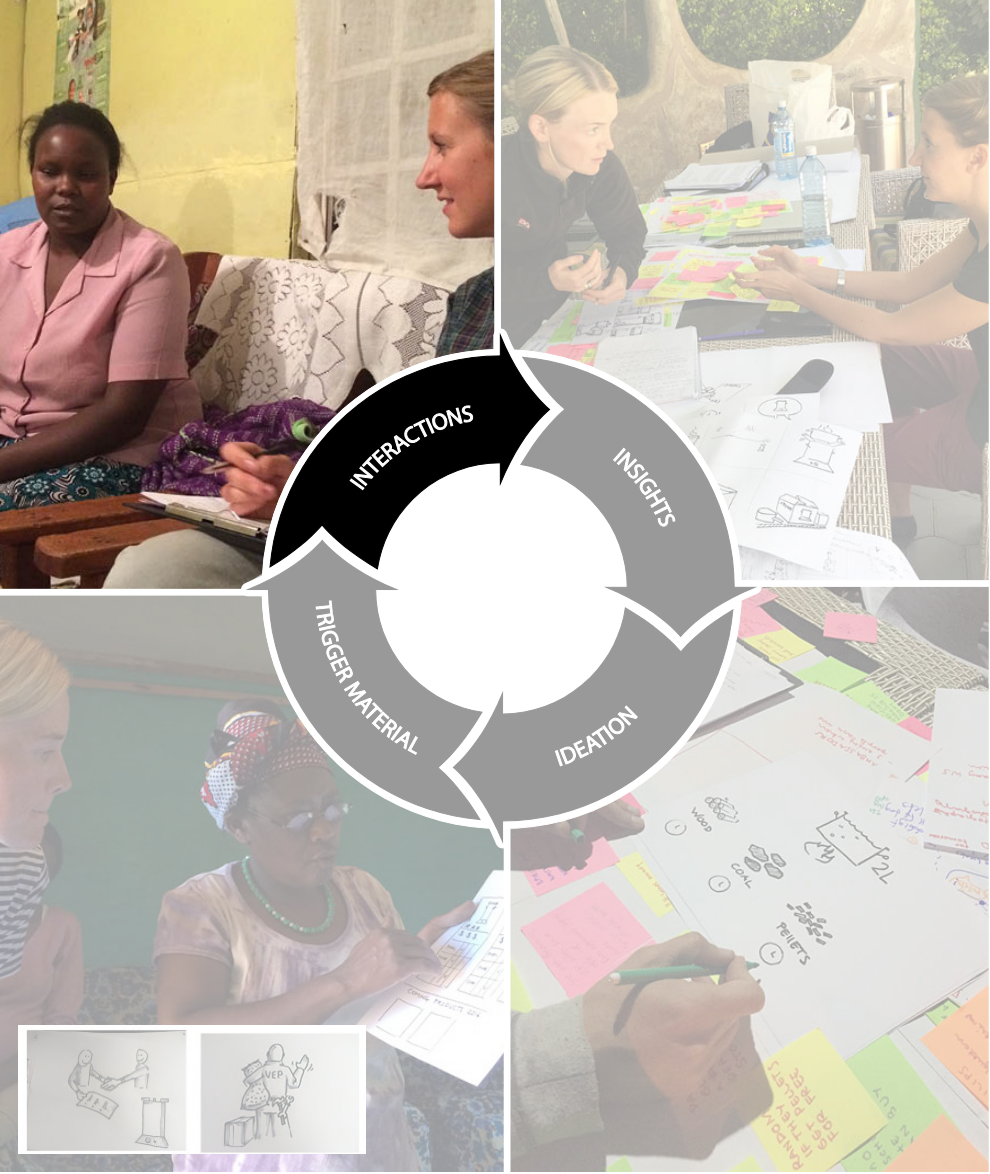
\includegraphics[width=0.7\textwidth]{Iteration.png}
    \caption{In Nissar's model, a iteration consists of Interactions, Insights, Ideation and Trigger material.}
    \label{fig:iteration}
\end{figure}

\begin{enumerate}
\item Interactions, where you are listening, the \textit{Explorative phase}.
\item Insights, which is where you use the Interactions in order to try to understand, the \textit{Understanding phase}. % better word+
\item Ideation, where you find possible ideas and when creation of new version of the app is done, the \textit{Design phase}.
\item Trigger material, where material is developed to test the outcome of our evaluation in the next round, the \textit{Trigger development}.
\end{enumerate}

The iterations should come closer and closer to a desired outcome. It is not always obvious what this outcome is. For each iteration, the process takes the project closer, from Why? to What? to How?, often with overlaps \citep{expedition-mondial}. See figure \ref{fig:iterationprocess}.

%\begin{wrapfigure}{r}{0.25\textwidth} %this figure will be at the right
%    \centering
%    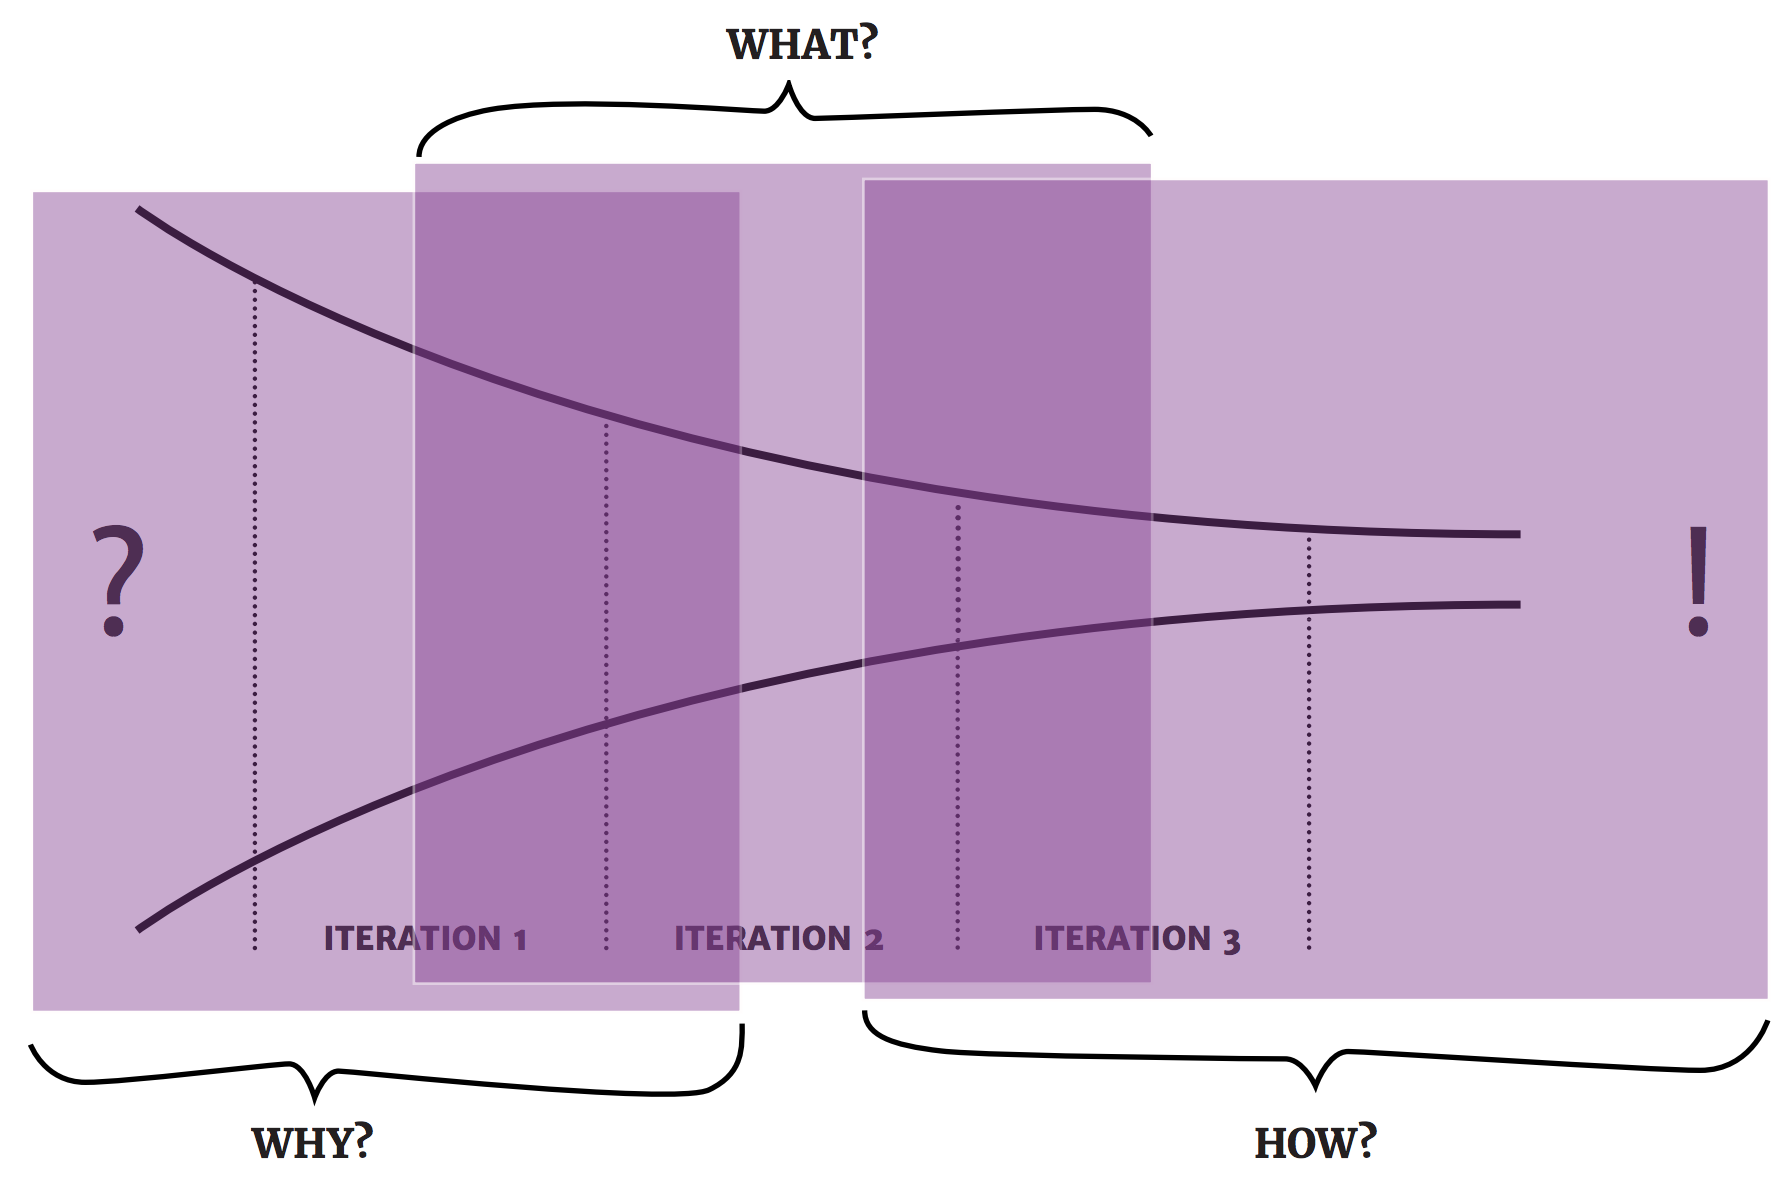
\includegraphics[width=0.25\textwidth]{IterationProcess.png}
%    \caption{Iteration process}
%    \label{fig:iterationprocess}
%\end{wrapfigure}

\begin{figure}[h]
    \centering
    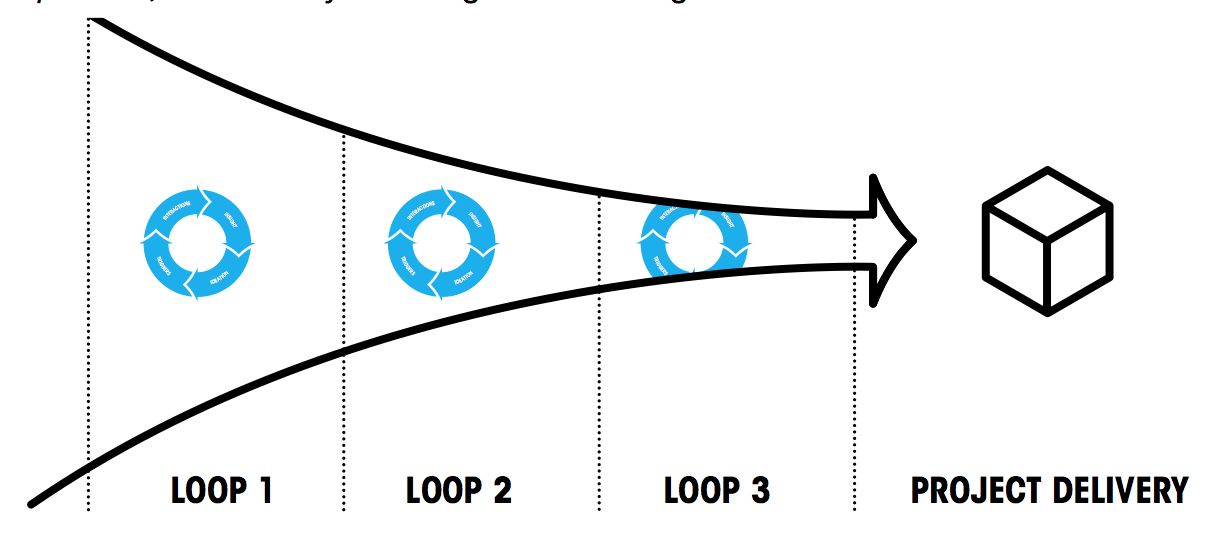
\includegraphics[width=0.8\textwidth]{projectLoop.png}
    %IterationProcess.png
    \caption{The iteration process consists of a number of iterations with different focus, starting with broad strokes, and narrowing down into a concrete product. Between iterations, there is an overlap in "Why?" and "How?", "How?" and "What?", which signals that there is a learning process which means conclusions may need to be quickly questioned as new insights emerge. This is especially important in projects where you work with an unfamiliar target group and there are several uncertainties and constraints.}
    \label{fig:iterationprocess}
\end{figure}

\subsubsection{Service Design Tools}

There are a number of popular service design tools that follows the five principles, e.g. how to make it user-centered. One is Customer Journey Map, in which an activity (like hosting a youth session) is broken into Before, During and After. Another method is Personas, which \textit{exemplifies} thought users of the app into people with names, having realistic character traits and opinions. The persona's neeeds can then be thought of when designing. An alternative to Personas are Need groups, where thought users are broken down by their different needs. Instead of designing for a specific person, you design for a person with a specific need. The advantage of Need groups, are that it accepts the view that the same person (Persona) might have different needs, depending on situation. The 5 Why's is a simple method used to dig deep into understanding the interviewee. Variants of the question "Why?"" is repeated five times as a rule of thumb, to understand underlying motives. This method is called "Why-why-why" within interaction design \citep{lowgren}).

Tools to create and reflect can be done via certain work methodology. When you structure and inspire brainstorms, you can ask "What if...?" and do Co-Creation, meaning doing ideation together with stakeholders or users. To create, agile development can be used, which is often suitable for software engineering. The manifesto for agile development is \citep{agile-manifesto}:

\begin{itemize}
\item Individuals and interactions over processes and tools
\item Working software over comprehensive documentation
\item Customer collaboration over contract negotiation
\item Responding to change over following a plan
\end{itemize}

An example of an agile methodology is \textit{SCRUM}, where a project is divided into several iterations similar to a service design approach of sequencing, but also introducing consepts like retrospectives (reflecting on one's work) and sprint demo (demonstrating the results of the iteration to stakeholders) \citep{kniberg}.

There are also some service design best practices: interviews are often done via open questions (encouraging stories) and dialogue can be facilitated with a questionnaire guide. In workshops, post-its are often used, and followed up with specific questions. Service design methodology encourages taking pictures, filming and recording audio, benefiting the analysis done afterwards \citep{expedition-mondial}.

%\input{theory/design/service-design/social_innovation}

%\subsubsection{Service Design Thinking}

%\input{theory/design/service-design/methodology}

%\input{theory/design/service_design_stoff}


  \subsection{Digital Service Design} \label{digital-service-design}

The method combines the benefits of Service Design, Agile Methodologies (namely SCRUM) and Interaction Design. Its purpose is to contribute a holistic approach to the digital design solution for a specific target group. The methodology was co-created by the current author and Expedition Mondial for the master thesis \citep{nissar}.

\subsubsection{The 4 stages of a "Service Sprint"}
In Digital Service Design, an \textit{iteration} is called a \textit{service sprint}. Each iteration includes four steps: insights, ideation, trigger material and interactions. Each steps borrows a number of best practices from agile development or interaction design. There are also new methods, like how a \textit{field hackathon} includes \textit{mini service sprints} each day. Below, the four steps are presented.

\subsubsection{Step 1 - Insights: Analysis, Retrospective \& Stakeholder feedback}
  Insights consists of \textit{analysis} (service design), but also a \textit{retrospective} (SCRUM) and \textit{stakeholder meeting} (service design). In the analysis, the app is evaluated (in terms of interaction design - pleasurability, usability, utility and desirability), and quantitative data is processed (often by clustering data points) and compared with qualitative data (quiz results and questionnaires). This produces an analysis overview of the result. In the \textit{retrospective}, the design process is evaluated ("start doing, stop doing, continue doing"), and changes to the design process are suggested for the following iteration.

    Both the result analysis and the design process analysis is then presented during two stakeholder meetings (service design), structured as \textit{sprint demo}s" (SCRUM), with the purpose of getting feedback. The first "Expert meeting" informs the next iteration's design process, while the second "Partner meeting" informs the next iteration's delivery. From the new insights, a \textit{product backlog} (SCRUM) is converted from needs and ideas into \textit{stories} balancing 1) user needs and 2) stakeholder needs.

\subsubsection{Step 2 - Ideation: Planning Interactions and Delivery}
  Ideation consists of doing \textit{sprint planning} (SCRUM) for the trigger material (a \textit{lo-fi} or/and a \textit{hi-fi prototype}) and the interactions (where tests and workshops and field visits happen).

    \begin{itemize}
    \item Trigger material
      \begin{enumerate}
      \item Ideas are formulated which would satisfy the user needs. This is often a iterative process, which happens in dialogue with chosen experts and entrepreneurs in technology, design and education.
      \item To plan implementation of the ideas, every technical task are laid out, measured in time and prioritized. The least prioritized tasks can thus be cut or moved to the next iteration, in case it is necessary.
      \end{enumerate}
    \item Interactions planning
      \begin{enumerate}
      \item If the technical planning has been realistic, it is time to determine what this iteration's interactions should look like. How will this be tested?
      \item The interactions activities are chosen (what, how, when), so that these are communicated to the local partner, who may schedule the days that will be visited, and solves the needs to the best of their ability.
      \end{enumerate}
    \end{itemize}

  \subsubsection{Step 3 - Trigger Material}
  Trigger material is about preparing the interactions (field visits, interviews, app tests, workshops) and creating the low-fidelity (pen and paper) and high-fidelity prototype (developed app) to be tested with the users. To track the progress and plan effectively, each day starts by a daily stand-up, where today's targets are set, ending by reflecting if the targets were met. If they were not, either the design process needs to change, or something needs to be cut short.

  \subsubsection{Step 4 - Interactions: with "Service Mini-Sprints"}
  Interactions always consists of a sprint demo with the users with the low-fidelity or high-fidelity prototype. During the development process, these are \textit{formative tests}, while for final app evaluation, this is a \textit{summative test}. \textbf{Group tests} are facilitated as workshops. Often, a scenario is presented, devices are given, results are submitted, followed by an open discussion. \textbf{Individual tests} are facilitated in the field (using the before, during, after technique). I observe how the coach does the job today, tests and observes if the app fits into the process, followed by an interview.

    These tests always informs what steps to be taken next, both in terms of app development and interactions. Instead of waiting for the next iteration to do these changes, often a so called Service Mini-Sprint is done.

    In a \textbf{service mini-sprint}\label{mini-sprint}, the insights gathered during the day allows for last-minute adjustments of coming pre-planned workshops (\textit{co-define}, \textit{co-create} or \textit{co-refine}) or field visits (change of interview questions), that can sometimes happen the same day. To take advantage of the precious time with the coaches, at the end of the day, app improvements are made and tomorrow's design process revisited. This means, that already the next day, an improved version of the app can be tested. Similarly, improvements to a workshop format can be improved. These mini-sprints allows for very fast iterations, which can sometimes accelerate the outcome of the visit.


  \subsection{Hybrid App Development}

The history of app and web development is rich and increasingly intertwined. First, websites were developed for desktop only, and when smartphones became popular, they were made responsive.

With today's possibilities of native mobile development or developing a native app using web technologies, there are numerous viable alternatives available if an app should function on several devices, depending on budget and preferences.

One of the main argument for developing an app in web technologies, is that the whole application, including the server, can be written in one programming language, JavaScript (full-stack).

Tools such as Apache Cordova can compile JavaScript applications into native apps. Thus, they can appear on Apple iOS and Android Play Store, as well as on the web, or installable offline on a smartphone from the computer.

JavaScript is developing rapidly as a language, as well as its ecosystem of frameworks and tools. Frameworks have emerged and matured, like Meteor.js, which makes building full-stack applications in JavaScript reliable and fast.

Previously, web hosting has been troublesome for JavaScript server applications. Today, tools such as Meteor.js and Heroku have introduced free and paid hosting for such applications, with smart bindings to code platforms such as GitHub, which makes collaboration and version handling easy.


  \subsection{Data Analysis}\label{sec:data-analysis}

This section presents relevant methods for analysing qualitative data and quantitative data.

\subsubsection{Qualitative Data}

Below, methods for analysing qualitative data are presented. In the research phase, Personas or Need groups are methods to analyse the though users of a product or a service. A Customer Journey Map supports understanding of how such users interact with a product or a service. Getting feedback from users involves getting ideas or suggestions for improvement of a product or a service. To analyse these, a sprint backlog is used to keep track of the priority of such feedback. If the features are then successfully implemented in the eyes of the users and stakeholders, can be tested using a sprint demo, where feedback is gathered for future work.

\subsubsection{Persona or Need groups}
When creating a product or a service, it is important to understand who you are designing for. Since the intended users might not always be around during the development phase, it helps having a clear mental image of the user. Fictional examples of users are one method to do this, either by using personas or need groups.

A \textit{persona} is a fictional character, created to give an example of the user who you are designing your service for \citep{stickdorn}. Depending on how broad the target group is for the service you are building, the persona might have several different needs. Then, dividing the though user groups in terms of designing for their different needs than their character traits might be more helpful \citep{expedition-mondial}. Dividing users by needs, if called forming \textit{need groups}. A need group (like "The beginner" or "The planner") can be described by their behaviour and their need.

Personas and need groups should be developed from research insights gathered from interviews or workshops with users and stakeholders \citep{stickdorn}.

\subsubsection{Customer Journey Map}
A customer journey map is said to provide a vivid but structured visualisation of a service user's experience \citep{stickdorn}. A typical customer journey is multi-channel and time-based, see figure \ref{cjmExample}

\begin{figure}[h]
    \centering
    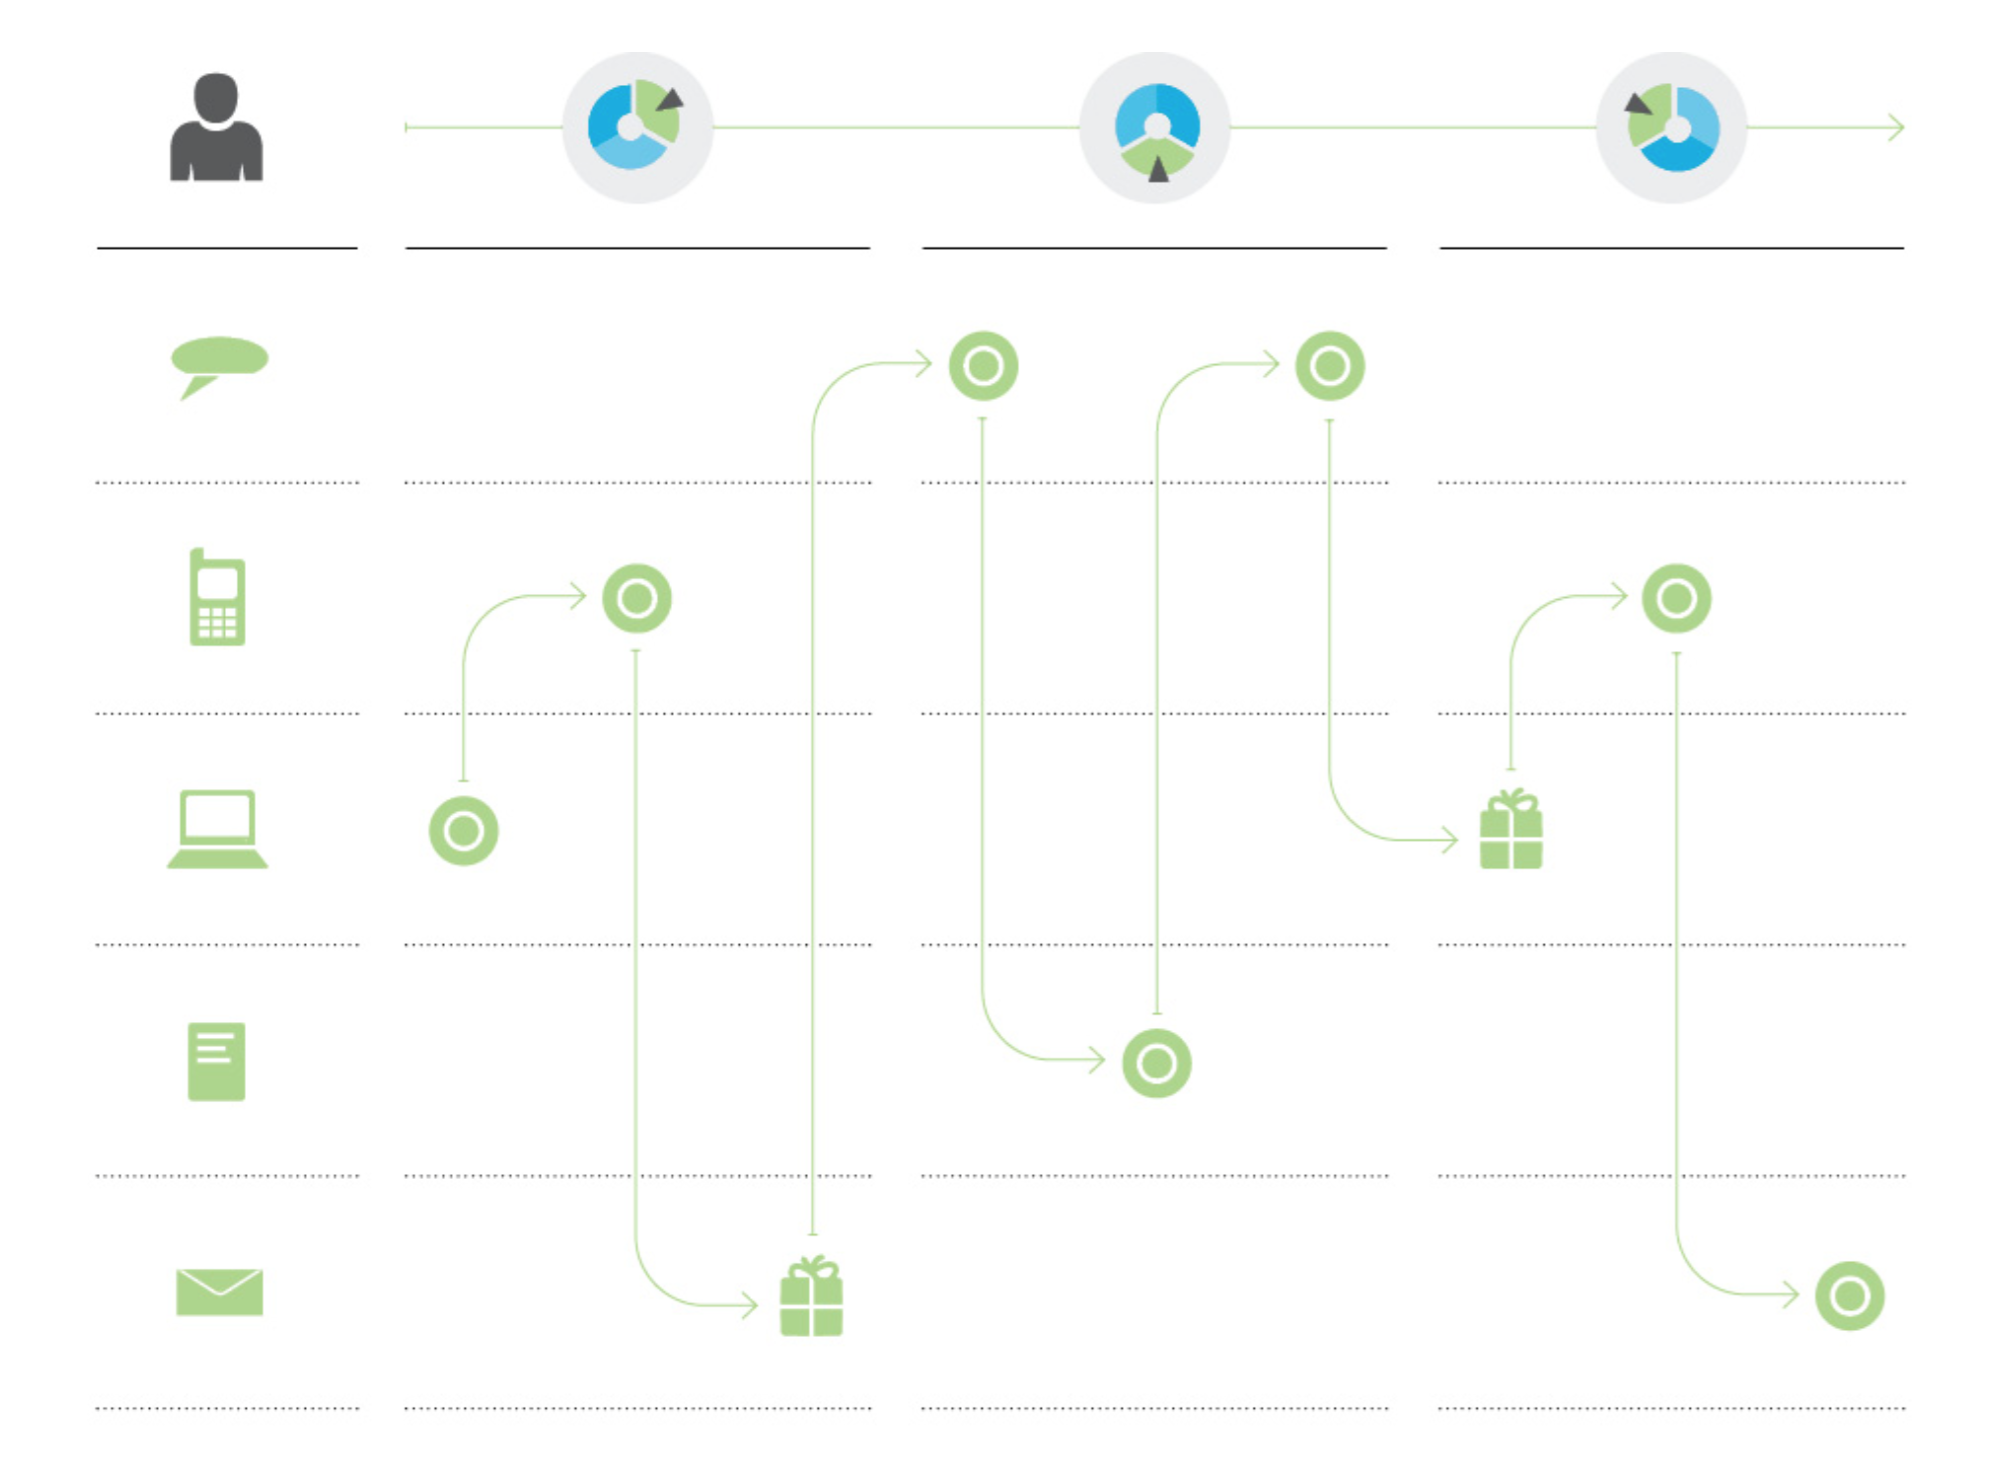
\includegraphics[width=0.7\textwidth]{analysis/cjmExample.png}
    \caption{General example of a customer service map. The map is divided by channel (could also be by a persona) and time (in this case before, during and after using a service).}
    \label{fig:cjmExample}
\end{figure}

The customer journey map is beneficial both for understanding a user's touchpoints with a service, and also for collecting and analysing stories which explain why the journeys happened as they did \citep{stickdorn}.

\subsubsection{Sprint Backlog}
During product development, to do a sprint backlog is a kind of data analysis. When a high altitude of ideas and feedback has been gathered, a sprint backlog is a list sorted with the most important and urgent items on top.

To work through ideas in a structured way, requests are categorized into what is called "stories". A good story answers "As a [user type] I want to be able to do [feature] so that [benefit]". Each story can then be broken down into todos ("What needs to be done in order to satisfy the story?"). During the sprint planning, the most important stories and todos are identified. By analysing and then working on the most prioritized story and todo, you ensure that you are always working on what is most important for the success of the project.

At the end of an iteration, as much as possible of the sprint backlog has been taken from "Not done" to "Done". The things not done, can either be moved into a product backlog (to later be added into an upcoming sprint backlog) or removed (they were not important enough).

\subsubsection{Sprint Demo}
A sprint demo is an effective way to analyse the product created after an iteration, from the perspective of the users and the stakeholders. \cite{kniberg} says that a well executed sprint demo attracts vital feedback from stakeholders, and ensures that todos are 100\% done. A sprint demo does not need to be complicated: the product is shown and tested with users and stakeholders, getting feedback for the next iteration. But without it, it would not be possible to know if the work done has satisfied the needs of the end users, or what the stakeholders thinks is important for future work.

\subsubsection{Quantitative Data}
Below, methods for analysing collected quantitative data are presented. The first method is correlation, but if multiple variables needs to taken into account, logistical regression can be used. As both of these are statistical tools, they rely on statistical significance in order to be trustworthy. In small-scale app tests, such amounts of data might not be sufficient.

To find trends or oddities in a small data set, visualization techniques to discover the data by hand might be more beneficial. To enable a visualization, the data needs to be collected, enhanced, mapped and rendered. When rendered, a suitable rendering of a multiple-variable data set might be parallel coordinates, which shows correlations graphically, and can be made filterable by user interaction.

\subsubsection{Calculating Correlation in Google Sheets and R}

The process is to calculate and compare means on a "control"  with a response variable.

It is clear that analysis in Google Sheets can only go so far. It can be greatly helpful to sort by multiple columns (e.g. first by Manual?, then by School level, then by Quiz 3). However, it takes a long time to filter the data on multiple parameters, and the work easily becomes tedious. For some applications, it may not be viable to discover the data using this approach.

In Google Sheets, color scale can be used to give different column values different colors, see figure \ref{analysFarg4}. It is still hard to compare all of the axises towards all the axises, and it is not a scientific approach.

Even in R, it is cumbersome to do statistically with all of the axises against all the axises. It is however possible to in both Google Sheets as well as the R programming language. Psuedo-code in R would be:

\begin{verbatim}
x1 = c(1,2,3,1,5,6)
x2 = c(2,3,4,NA,6,7)
cor(x = x1, y = x2)
cor.test(x1,x2)
\end{verbatim}

In R programming language there are more powerful tools for visualizing the correlation, e.g. using a "Correlation Heatmap", see figure \ref{fig:corrHeatmap}. Psuedo-code in R would be:

\begin{verbatim}
random_matrix <- matrix(rnorm(100), nrow = 10, ncol = 10)
random_matrix[1,1] <- NA
colnames(random_matrix) <- paste("V",1:10)
cor_mat <- cor(random_matrix)
heatmap(cor_mat, keep.dendro = FALSE)
\end{verbatim}

\begin{figure}[h]
    \centering
    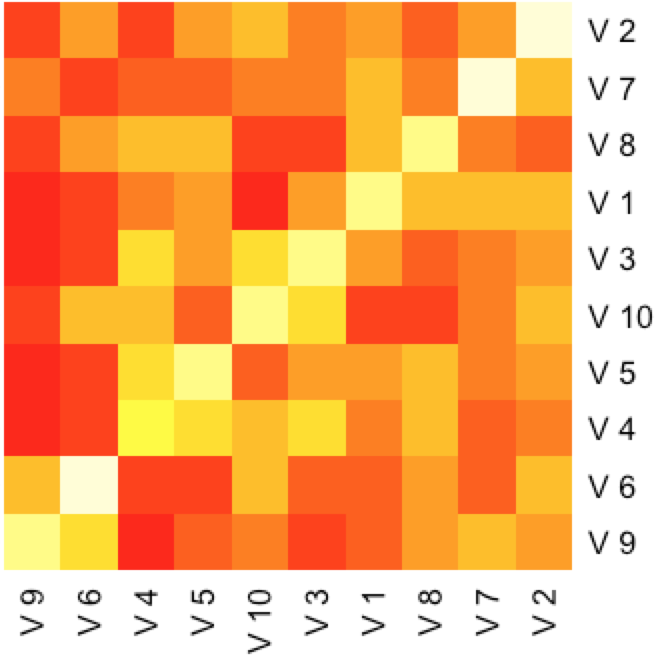
\includegraphics[width=0.7\textwidth]{analysis/rStatisticalAnalysis.png}
    \caption{Heatmap showing correlation, axis against axis, using example data. The more red a segment is, the bigger is the correlation between those two axises. You can see that in this example, there is a big correlation between for example V4 and V9.}
    \label{fig:corrHeatmap}
\end{figure}

\subsubsection{Calculating Logistic Regression in R}

A limitation with correlation is that only two dimensions can be compared with each other at the same time. What if we want to find a correlation between quiz score and gender \textit{and} age?

To do this, Logistic Regression is helpful if our response variable can be a logistical dimension (e.g. women or male, used manual or not), while linear regression needs to be used if it is a linear or nominal scale (e.g. age and city respectively).

In either case, the first step is to determine a response variable: the variable to compare against, e.g. is there a difference between men and women? In this case, it needs to be a quantitative measure of: "Have you learned anything?".

If one more variable is added, e.g. also adding if a manual was used, this is called the "control". It is possible to add as many controls as possible.

If linear regression, then it is needed to determine a quantitative measure of ("How much have you learned?").

In Google Sheets, this is not effective to do. R, however, is a very suitable tool. First, the data is loaded, e.g. as a CSV file. Then, we tell R which the N/A values are, e.g. "N/A" or "Vet ej". We use this to filter the data. Then, each column we want to use is converted into a factor.

When factors, a model can be created, e.g. using the General Linear Model. A different family can be selected, e.g. binomial.

Then it is possible for R to show this data, showing the coefficient, the Pr value, and others. See code below.

\begin{verbatim}
mydata <- read.csv("Development/R/quizResults.csv", na.strings = c("N/A", "Vet ej"))

mydata$y = ifelse(test = is.na(mydata$Quiz.9..y.n.1st),  yes = 0, no = 1)

mydata$y <- as.factor(mydata$y)
mydata$Help <- as.factor(mydata$Help)
mydata$Sex <- as.factor(mydata$Sex)

mymodel <- glm(formula = y ~ Pre.test.score + Sex, data = mydata, family = 'binomial')

summary(mymodel)

plot()
\end{verbatim}

For analysis, looking at the summary, coefficient (e.g. -1.0704) shows either a negative or positive correlation (in this case -7\%) for what to compare with as a response variable.

To be significantly significant, a common measure is that the Pr value ("the p-value") needs to be higher than 0.05. If the p-value is higher than 0.05, meaning it is significant with a 95\% probability.

\subsubsection{Visualizing and Analysing Multi-Variable Data with Parallel Coordinates}

\cite{timo-ropinski-liu} describes the "visualization pipeline", generating an image from data:

\begin{enumerate}
\item Data acquisition ($\,\to\,$data are given)
\item Data enhancement ($\,\to\,$ data are processed)
\item Visualization mapping ($\,\to\,$ data are mapped to for example a geometry)
\item Rendering ($\,\to\,$ images generated)
\end{enumerate}

% Timo Ropinski, Scientific Visualization Group, Linköping University, TNM067 - Scientific Visualization, 9/12/2014)
% https://drive.google.com/drive/u/0/folders/0BzlK1PD8EE75bHIxcXRQNWpRMm8

Data acquisition presents how data was acquired. Data enhancement explains how the data was processed. Visualization mapping is the process of mapping data to e.g. a geometry. Finally, rendering allows images to be generated, presented in 2D. This image can then be analysed.

What rendering to do, depends on the situation. In a multiple-variable data set, parallel coordinates is often a suitable visualization, especially if there is a lot of data for each axis.

Parallel coordinates allows you to see relationships and trends between dimensions. They can be seen by a positive or negative relationship (correlation or invert), or no relationship at all (random) \cite{une-terre}.



\section{Setting and Research Context}

In setting, the people that are involved with the project is presented. In research context, the physical environment is described.

\section{Collaborators for the Master Thesis}\label{sec:collaborators}

Collaborators in the project are the current author, supervisors, stakeholders and experts. Below, the responsibilities of these are more clearly laid out.

\subsubsection{The Current Author}
It is needed to take on several roles in the project by the current author: most notably that of a project leader, designer and developer. It is needed to balance stakeholders' different opinions and requirements, and caring for the vision in order for the project to be successful (see section \ref{aGoodDesigner} A Good Designer).

There are two groups, with the current author included in both of them, which gather at the end of each sprint for a check-up meeting. The Expert group consisted of Expedition Mondial and LiU Innovation. Expedition Mondial could help with the design process, and LiU Innovation could offer input on social innovation. The meetings mostly lasted for one hour. The Partner group consisted Iliana Björling from YoungDrive, and Lena Tibell and Konrad Schönborn from Linköping University. In Partner meetings, The Insighs from each iteration was presented and discussed. Then possible decisions were laid out, followed by discussing the alternatives. Outside of these groups, these people can also give advice in certain situations. For specific areas, there are also some experts which have been beneficial during the projects. Below, the whole team is explained: % Then I tell them about which decisions has been taken and why.

\subsubsection{Supervisors}
The supervisors are from YoungDrive and Linköping University. The YoungDrive team consists of Iliana Björling, founder of YoungDrive, and Josefina Lönn, country manager in Zambia. They are both helpful in giving knowledge on the entrepreneurship education program, and giving support. The Linköping University team consists of Lena Tibell, Professor, and Konrad Schönborn, Doctor, within the Department of Visual Learning and Communication.

\subsubsection{Stakeholders}
The stakeholders are considered YoungDrive and Plan International. \textbf{YoungDrive} is the client of the work, and their needs should be satisfied. This person is mainly represented by Iliana Björling, who is part of the YoungDrive Strategic Management Team. Using service design, the project leaders in Uganda and Zambia, are also considered stakeholders: Josefina Lönn in Zambia, and the two co-project leaders in Uganda. Finally, the most important stakeholder of all according to service design, is the actual users: the coaches. They should be the main consideration of the work.

\textbf{Plan International} is the organization allowing for all the interactions with the end users in Uganda. A similar organization is operational in Zambia. They are the ones that are providing facilities, organizes transport, etcetera. They in turn, have the organization Community Vision, which organizes the coaches. If Plan International or Community Vision does not appreciate of the project and the collaboration, then the interactions with the coaches will not be possible.

%\textbf{Linköping University} is a stakeholder, as the supervisor (Lena Tibell) and examinator (Camilla Forsell) determine if the work is a valid master thesis or not. Also, LiU Innovation is interested in supporting continued work with the project, and their representative Peter Gahnström gives advice on social innovation and how this project can continue in the future during expert meetings.

\subsubsection{Advisors}
Since the development country context is new to the current author, there are also specific experts advised in the project. For design process, Susanna Nissar and Erik Widmark from Expedition Mondial has supported with all of their knowledge within service design. Julien Tantege, Research Specialist at Grameen Foundation, has been kind to offer support before and during the work, sharing their insights from related work, and giving feedback during ideation. She has experience doing technical development for rural areas. For pedagogical development, Henrik Marklund from edtech startup Knownly in Sweden has given support with regards to building skills within digital learning. For feedback for how the work relates to social innovation, Peter Gahnström at LiU Innovation has offered feedback.


\subsection{Research context} \todo{Include a photo or two showing the setting of the workshops / data collection}

The biggest challenge with regards to time constraints and cultural differences is that it is difficult to understand the audience.

Therefore, the whole design and development process will take place in Uganda, with several interactions with the intended users.

The work was carried out from Hive Colab, a co-working space and an innovation hub.

The interactions took place in either Uganda or Zambia, in the locations where training of the coaches and youth takes place.

There were a number of resources made available to support the work, e.g. the \textit{YoungDrive manuals}.

Each youth is given a \textit{Participant manual}, describing each week of the 10-week YoungDrive program.

Coaches are also given a \textit{Coach guide}, which describes how to carry out and teach each week's topic during the youth training.

Working mainly from Kampala, because that is where YoungDrive is situated, means that there is still a long distance to the coaches and youth in Tororo, which is located near the Kenyan border.

Another challenge with being in Uganda compared to Sweden is that internet speed and access is worse, especially outside Kampala.


\section{Understanding the YoungDrive participants}

The following section describes roles, businesses, and coach descriptions for Uganda and Zambia.

\subsection{Roles}

The \textit{country manager} trains the project leaders. It is also the main person responsible for partnerships and the quality of the YoungDrive program in the respective country.

The \textit{project leaders} trains the coaches. They oversees the coaches, manages the coach training, and also collaborates with local stakeholders for quality assurance and to oversee daily operations.

The \textit{coaches} trains the youth. In Zambia, a coach only has responsibility for training youth in the YoungDrive program. In Uganda, this is called a \textit{Youth Mentor}, in contrast to being a \textit{Community Based Trainer (CBT)}, which also trains the youth in other programs and leads the youth saving groups. Most of the CBT's in Uganda holds sessions together with a Youth Mentor, or divides work between them, instead of being alone. The coaches are often volunteers, receiving a small scholarship from the partner organization. They are often business owners themselves. The coaches could be described as social entrepreneurs \citep{mitchel}. Many of the YoungDrive coaches (and youth) are driven by that their business can have an impact on their community, \textit{as well} as take them out of unemployment or increase their current livelihood.

The \textit{youth} are the ones receiving the training from the CBTs and the YMs, being encouraged to start their own businesses.

\subsubsection{Country Managers}

In Uganda, the country manager is Iliana Björling. She is located in the Uganda capital, Kampala, which is a strategic location because it is the same city in which the national office of the main partner, Plan International, is located.

In Zambia, the country manager is Josefina Lönn, who previously was project leader in Kampala, and has held all the trainings up to this point. Now, she leads the operations and has trained the coaches in Zambia, in the new role of country manager and project leader.

\subsection{Social characteristics}

According to statistics gathered by YoungDrive during 2015 evaluations, there are a number of considerations to make regarding the coaches in Uganda. This regards entrepreneurship experience, technical access, and language.

All of the Tororo coaches run a business (26/26 respondents), with a majority running more than one. This means, they do have practical experience of running a business outside of the YoungDrive coach training.

While all have a cell phone, smartphones are very uncommon - only 3 uses Internet on the phone, every day or weekly, mostly for Facebook or email. Regarding power, none (0/26) has power at home, 3/26 has solar, and only 4 can write on a computer. Taken together this means that their technical skills are low, and needs to be in consideration.

Regarding language, English can be used in the coach app. While about half of the asked Uganda youth can not understand (129/225), read (133/225) or write (132/225) English, most of the coaches in Uganda are proficient.

These characteristics can be used for youth and project leaders as well.

\subsection{Tororo businesses}

The coaches in Tororo are divided into three different regions. Based on region, income and experience, they run different kinds of businesses. \footnote{In Uganda and Zambia, a small-scale business is typically not registered. Thus, the coaches' definition of a business can be more generous.}

In Tororo, the coaches' businesses range from: ananas, water melon, onion, chili, bakery, catering, corn, beans, fabric, plastic products, bird farm, milk, fish, ground nuts, cabbage, tomato, hairdresser, sewer, shop and rice.

In Tororo, there are 2 Project Leaders. Christine's business ranges from: bakery, corn, pig farm and plastic products. Patrick's business ranges from: silver fish, beans, corn, and bird farm. In comparison, in Kamuli, there are 4 Project Leaders. Their businesses ranges from: selling office supply, boda boda, bird farm, pig farm, green pepper, corn, cabbage, tomate, aubergine, chipati ("bread"), chilli, and charging of cellphones.

Among the youth, the top 8 most popular businesses in Tororo, with 134 respondents, are corn, cassava ("potato"), saloon, fish, making of bricks, beans, brooms and rope. These range from 9 for corn (6.7\%) to 5 for rope (3.7\%).

\subsection{Zambia coaches}
The Zambia coaches in Kabwe are better educated, and have better access to technology, compared to the ones in Uganda. Regarding sociology, ages ranged from 21-39 years old (26.8 average). 3 were mentioned as being shy during the interviews. They lived from 10-90 minutes outside of town (33 minutes average).

Regarding motivations for being a coach, 50\% had an emphasis on benefiting the community, and 90\% had personal reasons. The following statistics has been derived from the notes of the Zambian coach job interviews \cite{yd-zambia-interviews}.

Care for oneself:
\begin{itemize}
\item Learn business %(7)
\item More skills %(2)
\item Get idea
\item Expand business
\item Benefit CV
\end{itemize}

Care for community:
\begin{itemize}
\item Empower %(2)
\item Teach business
\item Leadership
\item Share
\item Stop bad behaviours of youth
\end{itemize}

Regarding experience, 8 had trained youth before, 8 had been a leader before, 9 had business experience.

Regarding YoungDrive, they said they could handle training between 8-30 youth (19.8 on average) per group. They could have 1-5 groups per coach (average 3.0), totalling a range between 8-101.5 youth (average 59.8).

During the visit in Zambia, the coaches had not yet formed their youth groups, and started their own sessions.


\section{Study Design and Data Collection}

  As a computer expert with social skills needing to design and develop an app for a unfamiliar cultural and socio-economic context, it was needed to quickly become a good designer.

  The technical aspect of the project was but one. It was needed to learn how to develop hybrid apps in JavaScript that worked offline, and had an online back-end. However, those are merely the technical demands.

  It was needed to quickly become a good designer, not mainly from a perspective of graphic design or interaction design, but \textit{how} to explore, design, and implements what the user needs from the requirements "fun, user friendly, and good for learning". The approach used to learn design from these perspective was to read extensive literature, consult a diverse set of experts, and be humble and curious in interactions with the end-users and stakeholders.

  In the following section, the creation and implementation for a suitable design process is described, together with the study design and data analysis for each iteration of the project.

%Har gått igenom planeringsrapporten lite noggrannare idag och ser två saker som vi kanske ska borde fånga upp under arbetets gång.

% Under 2 Purpose står det ett upplevelsemål från Young Drive. Bör vi mäta detta upplevelsemål om det stämmer med deltagarnas faktiska upplevelse, d v s ska vi försöka få in det under 3 Research Questions?

% På våra avstämningsmöten borde vi också följa upp dina Research Questions så att kundinteraktionerna och servicedesignmetoden tyligt leder dig framåt mot dessa mål.
%* Reflektioner på vilka designprinciper som bör väljas? (utifrån kundinteraktioner)
%* Reflektioner angående tekniska begränsningar?
%* Reflektioner på processen?

\subsubsection{Creation of Design Process}
As there was a unfamiliar target group - mostly young Ugandians with little or no experience of smartphones - service design thinking would benefit true understanding of cultural context and in-depth empathy for the end users.

Tools and methodology in service design were chosen with the help of Expedition Mondial in Stockholm, who provided education and coaching.

At the same time, the end result would be a digital artefact (an app), which is not common in service design.

While this product could be though of as a service, the tools and methodology would benefit to borrow from Agile methodology and Interaction design.

I'm the computer expert kind of designer \cite{lowgren}, adjusted to agile methodology and interaction design, but aspiring to be a socio-technical expert. Expedition Mondial are experienced with service design, aspiring to be more of computer experts.

This led to the joined development of a Digital Service Design method, co-created by the both.

%Expedition Mondial helped with a method for creating a MVP of the digital support for the coaches, so that the app was developed from the perspective of the end users and the education and a "learning by doing" mentality.

%The suggested design process was designed with them after a start-up meeting on Skype, and an education day in Stockholm. During that day a crash course in service design was given, then creating a common plan for the future work based on my needs (see Appendix: Original Time Plan \todo{Add reference}). They also recommended service design literature. These were the methods chosen in each iteration.

The result is that the design and development phase in Uganda is an iterative process with the human in focus. The process is built on top of service design process and methodology, while in-line with digital design practices.

\subsubsection{Implementation of Design Process}
There were four iterations. The first iteration follows Service Design, not starting the app development, while the other three follows the new methodology, Digital Service Design.

In iteration 1, there is a very broad scope, without digital focus, where iteration 2, 3 and 4 introduces and narrows down the project into a digital solution.

Expedition Mondial gave support in each iteration, helping with refinements of each iteration as learnings happened along the way, and they were able to educate me during the different stages with methodologies whenever necessary.


\subsection{Iteration 1: Uganda Coach Visit}

% How was this iteration designed?

Following the service design sequencing, the first iteration had a very broad scope and truly is a service design iteration: "From your perspective, what is it like being a coach?". \footnote{A coach meaning either a Community Based Trainer (carrying out all the trainings), or a YoungDrive coach, depending on who was asked the question.} \cite{lowgren} was used how to start the project, meaning that the purpose was to get a preliminary understanding of all important aspects, and build relationships with all stakeholders.

%The project started with a startup meeting with Shifteh from Plan International in Kampala, together with Iliana. From there, I did research and met with Grameen Foundation and Designers Without Borders, before going to Tororo to research "What's it like being a YoungDrive coach?", and determining how advanced an app could be to solve challenges that the coaches face.

Insights depended heavily on interviews with all the stakeholders  (2 with Plan International, 3 with YoungDrive), and local experts (1 visit each at Grameen Foundation and Designers without Borders, 1 workshop with Mango Tree), since no Interactions with users had been made yet. Also, knowledge and connections were made with the Kampala tech scene as much as possible, from the new home and office in Kampala, working at the tech hub and co-working space Hive Colab.

Ideation were about creating a questionnaire guide for the interviews, a co-creation workshop using "Customer Journey Map", and identifying how the app test should be designed to test their existing knowledge (and be informed of the design preferences of the YoungDrive app).

Trigger material was the finished questionnaire guide (constructed with Expedition Mondial) a written plan for the co-creation workshop ("A day as a coach"), and a written plan for testing the quiz app Quizoid and the language learning app Duolingo, and a schedule for the interactions.

The interactions were focused on design ethnology, getting to know and learn from people in a different culture, namely the coaches. The focus was on the their needs, motivations, and context.

To accomplish these, four days were spent in Tororo, with one day of travel. There were four face-to-face-interviews,
one meeting with Plan, one meeting with the local partners, two workshops, one coach stay-over, and two youth session visits (one of the youth sessions are observable via figure \ref{fig:youthsession}.

\begin{figure}[h]
    \centering
    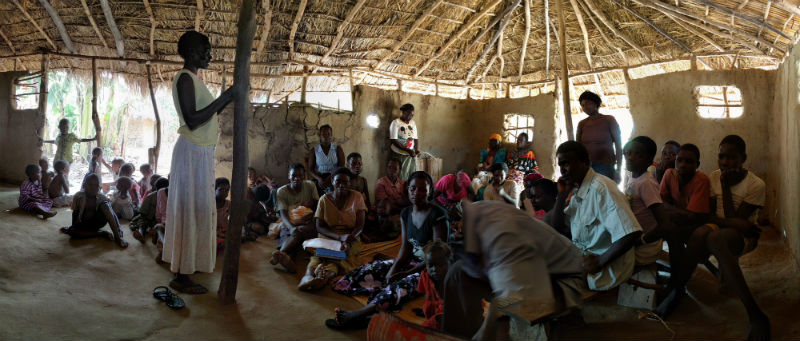
\includegraphics[width=0.7\textwidth]{youthsessionSmall.jpg}
    \caption{Photo from the location where one of the youth sessions were held. Here, a CBT in Tororo teaches youth in basic sales and marketing.}
    \label{fig:youthsession}
\end{figure}


\subsection{Iteration 2}

This time, the iteration has a more detailed scope, with a hypothesis on what needs the app should meet in the end, and create lo-fi and hi-fi trigger material to meet those needs.

A co-creation workshop started the interactions, followed by repeated app tests at minimum one session per day, always followed by a feedback round, so the app and the tomorrow's question set creation could be improved for the next day. At the end of the week, there was a co-refinement workshop of the current hi-fi material, and also lo-fi material for the new version of the app.

\subsubsection*{Creation of questions}
Project leader Josefina in Zambia refined Iliana's first question sets, prepared for my visit in Zambia. Josefina created question sets with Bloom at the back of her head, also taking into account the structure and the order of the coach manuals, what it means being a coach within the topic, and lastly scenarios.

\subsubsection{Trigger material used}
A hi-fi trigger material was done, a very basic quiz app, keeping it as simple as possible (see Application Implementation, Iteration 2). All of the devices (tablets and smartphones) that I had available were brought to Zambia.

I added Josefina's questions to the app, and installed the app to all of the devices. This process was repeated for all the days, Sunday-Friday.

\subsubsection{Design workshop \#1 in Zambia}
The coach training started with me having a design workshop with the coaches, not showing them the app that I had created. The co-creation workshop was made to identify important functionality in the minds of the coaches.

\begin{enumerate}
\item Since the knowledge about smartphones and apps were low, I started by introducing these topics.
\item All were familiar with Facebook, so thus I showed the Facebook app. Me wanting to know what the app would look like if the coaches would have designed the app, I first needed to train them how to design an app via drawing wireframes.
\item Using postits, they started with during limited time drawing the start view from the Facebook app.
\item Then, they were asked to draw what they thought happened on the friend icon click, drawing the view on another postit.
\item Then, the mission of the YoungDrive app was described. They were then divided into two teams, having limited time to draw the best imaginable YoungDrive coach quiz app they could. First, they designed the app from the top of their heads. They then pitched their results to each other.
\item On the next iteration, they were to suggest and design improvements how the app should be designed to improve learning, not only assessment. They then again pitched their results to each other.
\end{enumerate}

\subsubsection{Assessment via quiz}
At the end of each day, the app was used to test the coaches' knowledge. Each coach got either a smartphone, tablet or computer. The coach first took the quiz for the most recent session, and could then choose what to do next.

As there were no back-end developed, Josefina by hand documented the scores of each coach, writing the name of the coach, the session, number of correct answers, and what questions had been answered wrong.

Josefina then, when planning the next day, looked at the statistics, looking for trends that would inform the sessions for the following day.

She also evaluated the quality of the questions, before creating the new question sets for the next day.

\subsubsection{Experimenting with quiz before or after the session}
Since the coaches appreciated the app so much, we felt tempted to try what would happen with fun and learning if we tried using the app \textit{before} a session instead of only after. During the rest of the week, we continued, finally finding preferences and tendencies from the coaches, via observation, interviews, and survey.

\subsubsection{Experimenting with design of questions}
During the week, extra tests were done to test the following:

\begin{itemize}
\item Number of questions per quiz
\item Single-answer questions or multiple-answer questions
\item Framing of questions
\item Challenge level of questions
\item Determining what made a question hard
\end{itemize}

\subsubsection{Interviews with Josefina}
At the end of each day, an evaluation interview was held with Josefina. At the end of the week, a final interview was held.

At the end of Day 5, Josefina and I discussed what it would look like to not record the answers manually, but pushing the results online. A co-creation workshop was held, where she drew an Educator Dashboard.


\subsection{Iteration 3}

Because of the many research and functionality needs, the study design of Iteration 3 became very important. A lot of development and ideation needed to be done.

\subsubsection{Iteration 3: Purpose}
Iteration 3 had an even more detailed scope. Since the app now succeeds with the first use case, the coach training, now the focus could be on "learning at distance".

\subsubsection{Pedagogical model}
It was chosen that "Are you sure?" + Improve would be included in the hi-fi material, a flip-card approach would be tested as a lo-fi material, and to "record answer via voice" could only be presented as an idea during a field interview (experts said there would be usability issues, and the 1st-time smartphone user agreed). The Gold/Silver/Bronze method was included into the hi-fi material.

\subsubsection{Test on a Kampala entrepreneurship student}
Also, instead of only testing the app in Tororo, a test was held in Kampala, to get feedback from an entrepreneurship student.

\subsubsection{Test in Tororo}
As Plan International staff are not allowed to support visiting coaches in the field during local elections, the co-project leaders in Tororo were consulted to carry out the field trips, so that it was still possible to attend the youth group meetings.

For the interactions, a big app test was held, a group interview was held, and then they were divided into co-creation workshop groups, with a presentation in the end.

%Before the workshop, the wished functionality and goals were well formulated. It was also discussed beforehand how to best design the workshop, together with Linköping University and Expedition Mondial.

There was another partner meeting, with Plan International and Community Vision present. There was an app test with all of the coaches, "Testing the YoungDrive coach app", followed up by splitting into six workshop groups based on solving different problems discovered during the test.

The following day, there were three field visits to CBTs, observing how they prepared themselves for a youth session, and then testing the app for assessing and becoming prepared for a session.

After the app tests, it was tested with a lo-fi prototype that the coach thinks aloud about the question, \textit{before} receiving the multiple-choice answers. This approach proved to be great for learning, and could be a great addition to the hi-fi material. Interestingly, this test was done as a live quiz, and if the interviewee could not answer the question directly, the audience were asked and tested if they knew the answer (raised hands), and if nobody knew the answer, it was tested which of the multiple-choice alternatives they found most likely.

During the afternoon, we divided into 5 groups focusing on improving the app experience for the coaches.

On Wednesday, the coaches from the field visits were gathered for a workshop. The purpose was to see how they acted when given the challenge: "Get 100\% correct answers in one go, on the hardest quiz". A co-creation workshop ("Educator Dashboard") was held in parallel, with 3 CBTs and 1 project leader respectively.


\subsection{Iteration 4: Uganda Summative Test}

The focus of iteration 4 was a summative test. First, a pre-test was carried out in paper, including questions about the coach and an entrepreneurship quiz, based on a well-known study \citep{general-entrepreneurship-quiz}, see Appendix \ref{cha:pre-test}. During the test, this was the first time that the app could send data to the server. Data was sent whenever a quiz was started, and whenever a quiz was finished. The group was divided into two, the ones who brought manuals and they who did not. Those that had brought manuals, could use these with the app, see figure \ref{fig:appevaluation}.

\begin{figure}[h]
    \centering
    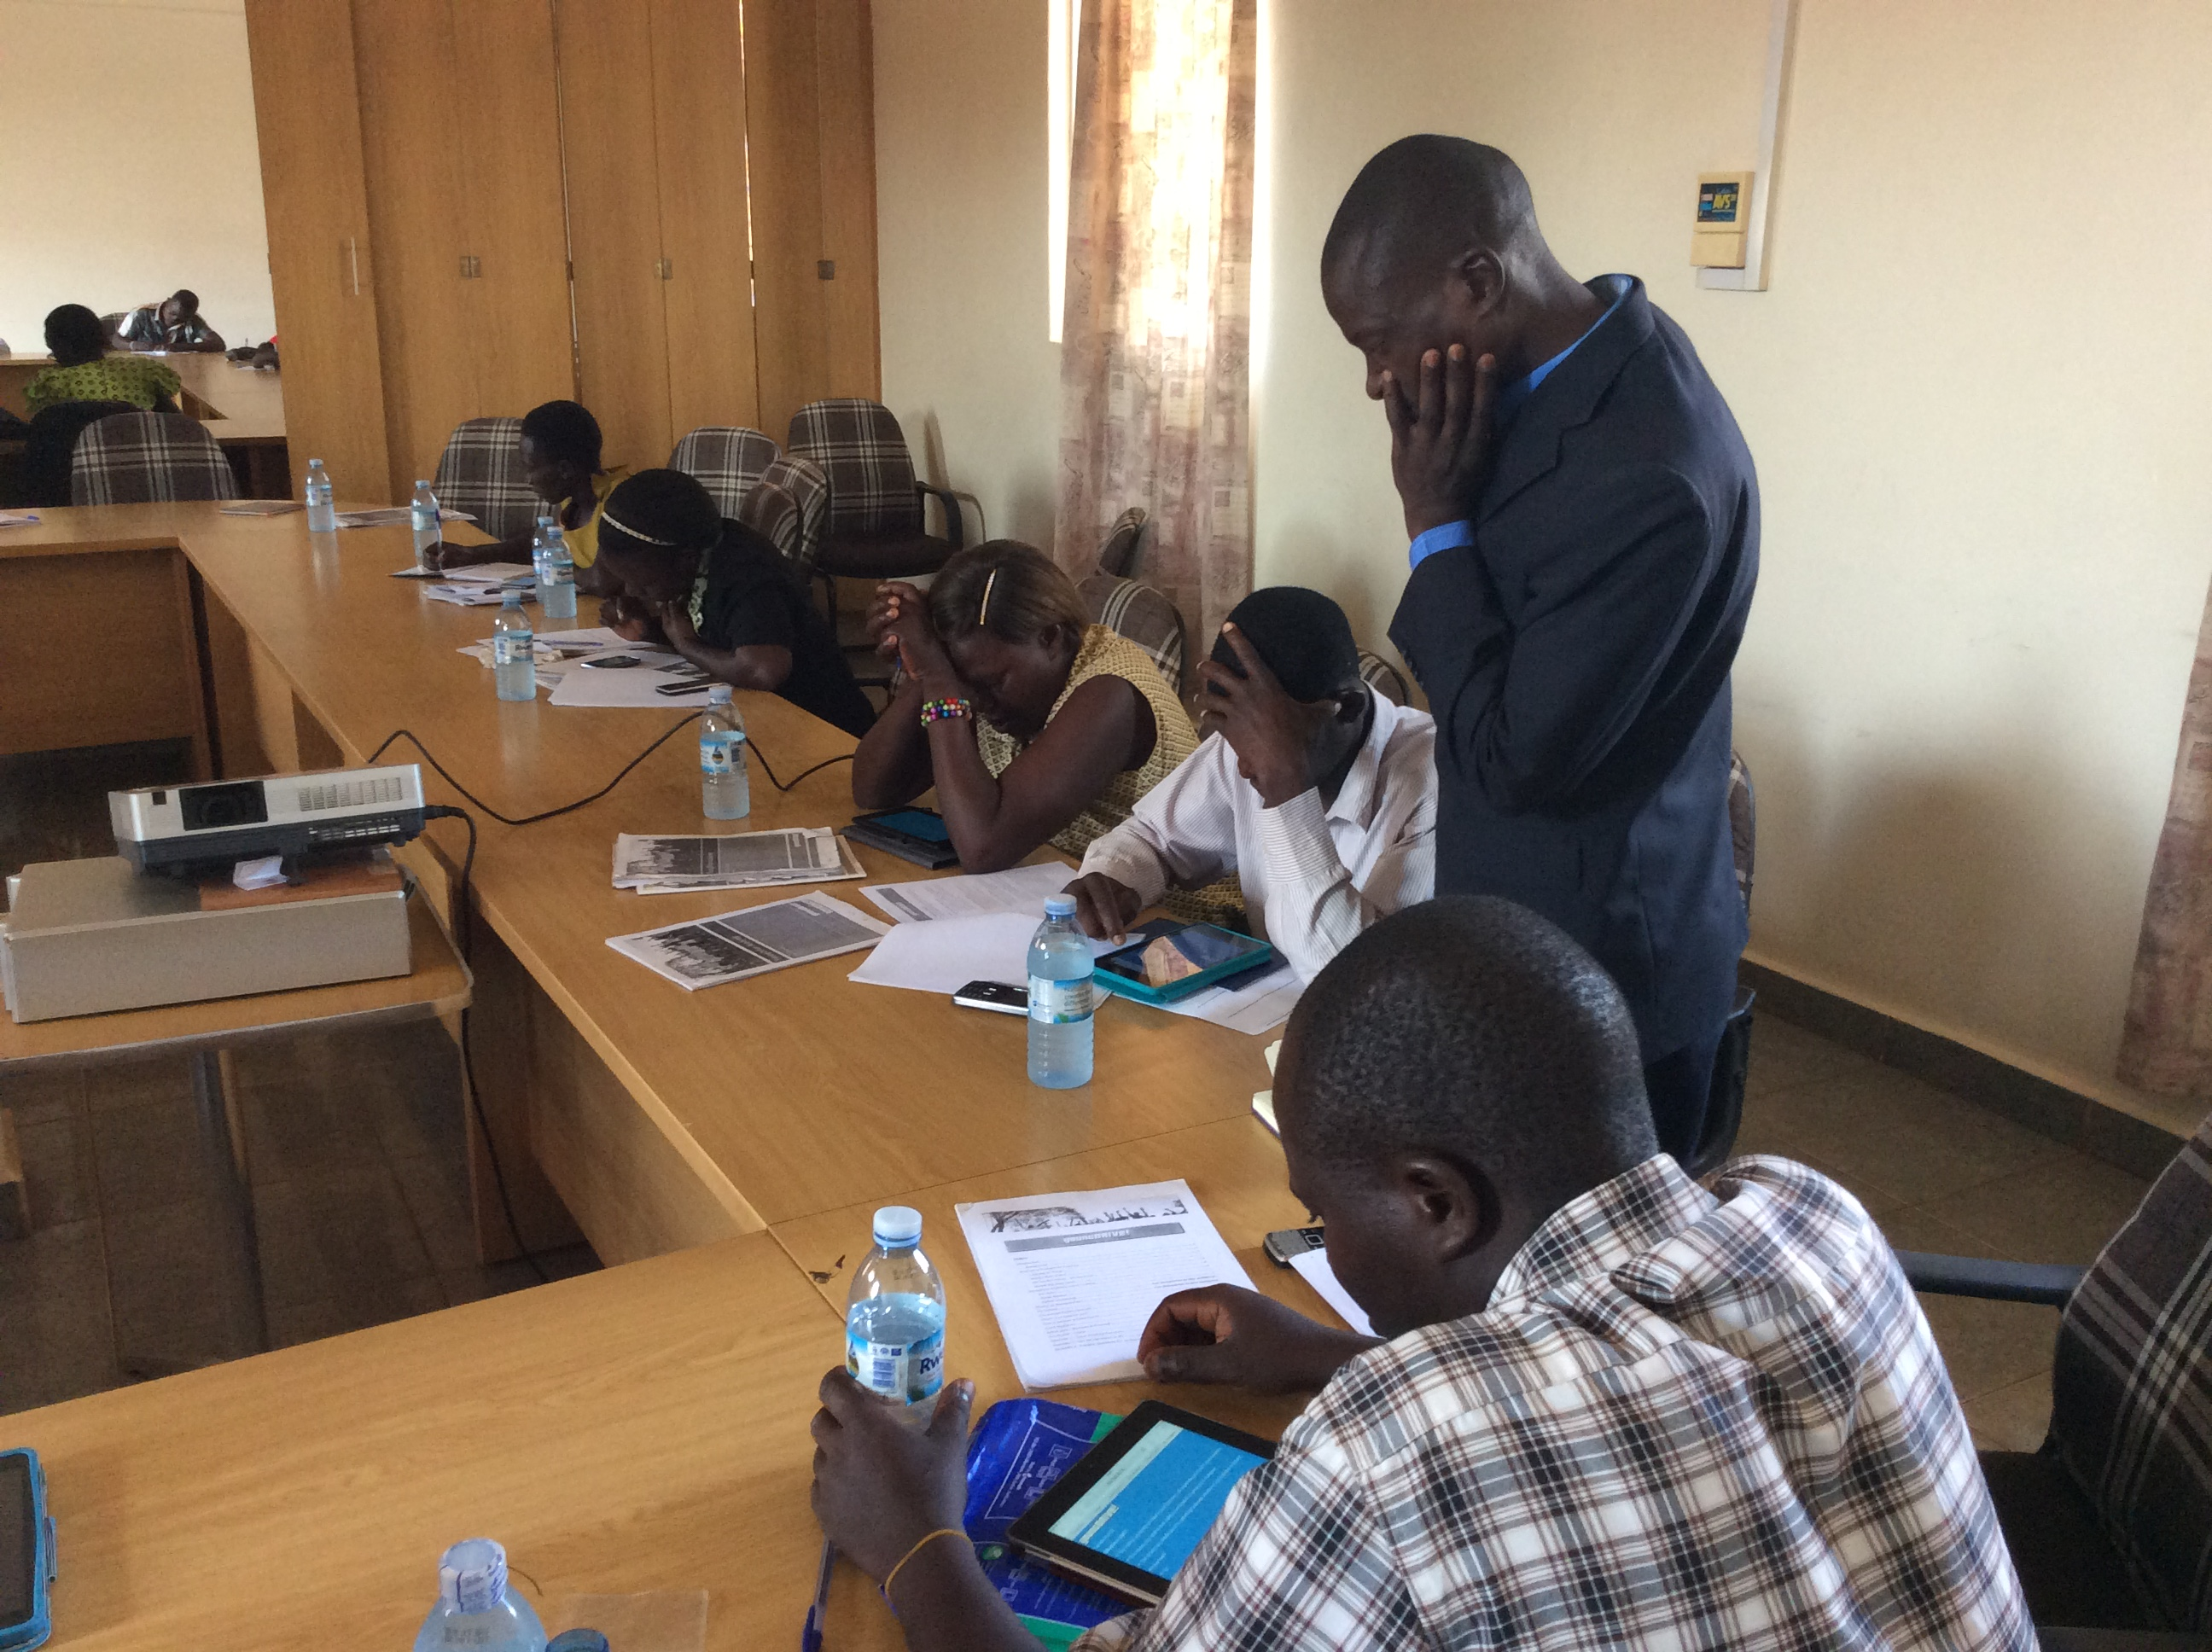
\includegraphics[width=0.7\textwidth]{appevaluation.jpg}
    \caption{Coaches answering the app questions for topic quiz 3 on Financial Literacy, and the coach guide quiz 9 on Action Plan.}
    \label{fig:appevaluation}
\end{figure}

After the test, every coach was divided into one or three groups, on random. In these groups, they were asked:

\begin{enumerate}
\item Why do you think you were correct or incorrect?
\item Do they like the app?
\item Are you stimulated by the app?
\item What did you like?
\item What did you not like?
\item When do you want to use the app?
\item When are you not able to use the app?
\end{enumerate}

To analyse the paper-submitted data, all of this was combined first into a Google Spreadsheet (the app results were also recorded in paper, but only as a backup). Data collection was done by the app itself, which pushes data to server whenever online (it saves quiz start, and quiz finish).

%The next day, a small app evaluation and co-creation workshop was held for the Educator Dashboard, and the final version of the app. Also, a test was done with the Plan Tororo staff.

%Back in Kampala, a presentation was held with Plan International. Back in Sweden, a presentation was held with the YoungDrive Strategic Management Team.



% Application implementation
\section{Application Implementation}

In this section, the prerequisites for the app is described, from the perspective of the user, stakeholders, and the developer.

\subsection{User Needs}

The technical constraints for the project, would need to affect the technologies used, if the project would be user-centered.

On the client side, the app would need to be mobile and web based, consider non-access to internet, and not use a lot of battery, to work for the coaches of YoungDrive.

That the app should be simple to use in this cultural setting leaded to design constraints and needs for evaluation.

\subsection{Stakeholder Meeds}

As the project was only three months, and the first month would be without digital development, time constraints were massive. However, to be able to answer research question \#2, evaluation needed to be done via data collection.

If no evaluation, there would be no need to write code, instead working with a lo-fi prototype using pure design tools. Now, a data-driven approach was needed to measure, and therefore an app needed to be developed.

On the server side, a database and API would be needed, to pull data from the database and push data from the client. Since internet was not always available, the client must be smart in its usage of pushing and pulling data. This would need to be investigated further into the project.

\subsection{Devices to be Used}
As most of the coaches did not have smartphones or tablets, four smartphones (3 Android, 1 iOS) and ten tablets (3 Android, 7 iOS) were brought from Sweden. All of these devices had a web browser and access to an app store. These were either donated, borrowed or bought devices. During the user tests, also using a laptop would be tested.

%\subsection{App/Web Development}
%Early in the project, it was thought that existing tools could be used, instead of building the app from scratch. E.g. using existing tools like Knowly or Typeform\footnote{examples include https://showroom.typeform.com/to/ggBJPd and https://showroom.typeform.com/report/njdbt5/dIzi} during the first iterations for understanding users, and during development e.g. the Typeform API (http://typeform.io/). The Typeform API allows developers to create surveys from within their own applications or systems.

\subsection{Choosing Frameworks for Creating the App}

A JavaScript framework helps and speeds up the creation of building web apps. In the start of the project, Meteor \citep{meteor} and Ionic Framework \citep{ionic} were both tested and compared with each other. It was decided that Meteor was the best way forward, partly because it would allow the app to be accessible on the web as well. %\todo{Add from mindmap}

React \citep{react} (a JavaScript library for building user interfaces) was chosen as the front-end framework, having integration with Meteor and being relatively easy to learn and fast for development.


\subsection{Iteration \#2}
Here, the work and result from iteration \#2 is presented.

\subsubsection{Staging environment using Heroku}
Needed when the Meteor free tier was removed. Connected to deploy from GitHub branches automatically. Could have benefitted from CI, passing tests before ready for production. Solved this by having a stage environment (since April 19th) where stage is YoungDrive-beta (branch Iteration 4), and YoungDrive is master.



For iteration 3, as components grew, there was a need for a client-side router. The Meteor plugin Flow Router was used, as it was very popular with good integrations.

For iteration 3, there was also a need to store data per individual, partly because the feature was prioritized from YoungDrive, but also because of the purpose of data collection. In order to store data per individual, a database and login would be needed. Because of technical difficulties, login and automatic data collection was not implemented until iteration 4, which can be read more about in the Discussion in \ref{backwards-capability}.

\subsection{Login}
To record data per user, would require login. This would be a usability issue for most problems, being 1st-time smartphone users. They need to find it intuitive, user-friendly, and be able to remember the password in the future. A lot of different suggestions were through the ideation phase.

The simplest login possible was chosen, after evaluation and discussion with experts: a 3-digit code, which was to be given to each coach during the test.

%Jag pratade med flera om detta, Expedition Mondial och Grameen. Från EM lärde jag mig att de trodde min idé med en färdiggjort lista med coachernas namn (vi vet ju vilka som är i Tororo) skulle fungera, och från Grameen fick jag höra om dera erfarenhet att de validerat använda samma approach, med en PIN (längre än 4 siffror dock), men att de inte nailat konceptet ännu, och att de också itererar på sin approach för nästa uppdatering av LedgerLink.

Meteor had limitations with their auto-login module, which is very fast to implement. It forces username and password, and instead I wrote the login myself. This was

To summarize, the front-end was not problematic, however, implementing server-client communication so that it worked online and offline, was.

%Tyvärr har också Meteor begränsningar med deras auto-login-modul. Den tvingar både användarnamn och lösenord, och har automatiskt registrering. Går det att stänga av? Jag kan skapa användare och lösenord åt alla, och funderade på hur jag skulle generera lösenord. Ett förslag blev att bara registrera deras förnamn, och sedan skapa lösenordet baserat på T9 med de 6 första bokstäverna utan att berätta det för dem. Sedan tänkte jag på det kulturella, att det kan vara oartigt med förnamn, och bestämde mig för efternamn istället. Hela namnet skulle bli för långt och krångligt.

%Helst skulle jag behöva gå runt Meteors standard-inloggning, och istället ha en enkel login-rullista som den ovan beskrivet, istället för att använda deras standard-lösning.

\subsubsection{Online and offline database}
If data was to be sent from the client to the server, there needs to be a database with Meteor Collections. An example app was made first, only using Meteor Collections. Meteor's use of Distributed Data Protocol (DDP), made app pushes feel immediate, even though data was not sent until there was Internet access.

However, it was found out that if it took more than 15 minutes to get online, the push would be aborted. For users that are seldom online, this would not be viable.

An offline database was needed, and the plugin GroundDB was implemented. As it was cumbersome to get right, pushing the data whenever online, and hard to test (needed to wait 15 minutes each time), this was not ready for the interactions until Iteration 4. As a consequence, until iteration 4 of the app, no results were saved online via the app whatsoever.



For iteration \#4, data collection was done by the app itself, which pushes data to server whenever online (it saves quiz start, and quiz finish). The server receives JSON data from the client, stored in the MongoDB database hosted on Heroku. Each data point is saved in a database called Results, with the signed in user (from the Users database). In the database, there are collections for Users, Quiz Lists, and Quiz Results.




\section{Data Analysis Theory}

%\todo{Lägg till overall data table}

%Methods to choose from for analysing (i.e. what I did during the interactions, to test and analyze my app)

%Partly data collection done via app, but also all the observations

The results from each iteration needed to be analysed, using the methods outlined in section \ref{sec:data-analysis}. Depending on the kind of activity and results gathered, different data is collected.

For qualitative methods, the output is almost always observation notes, which are then concluded into insights. These insights, can then sometimes be used in the below analysis methods.

For quantitative data, the output is almost always quiz results or data about the coaches. Before analysis, how this data has been processed is clearly described in chapter \ref{sec:data-analysis}.

Below, an overview of which data analysis method was used for what data is presented. The tools and iteration the tool was used in, is outlined below as a summary:

Qualitative data analysis:
\begin{enumerate}
\item Need groups and Personas (\#1)
\item Customer Journey Map (\#1)
\item Sprint backlog (\#1, \#2, \#3, \#4)
\item Sprint demo (\#1, \#2, \#3, \#4)
\end{enumerate}

Quantitative data analysis:
\begin{enumerate}
\item Correlation in Google Sheets (\#2, \#3, \#4)
\item Correlation in R (\#4)
\item Logistical regression in R (\#4)
\item Parallel coordinates visualisation (\#4)
\end{enumerate}

\subsection{Iteration 1: Uganda Coach Visit}

In iteration 1, the following activities were carried out and then analysed:

\begin{itemize}
\item Stakeholder interview (for Need groups)
\item Coach interview and field visit (for Need groups)
\item Workshop (for Customer Journey Map)
\item Smartphone test (for Need groups)
\end{itemize}

\subsection{Iteration 2: Zambia Coach Training}

In iteration 2, the following activities were carried out and then analysed:

\begin{itemize}
\item App test observations (for Sprint backlog)
\item Quiz results (for Sprint demo)
\item App design workshop: use case 1 (for Sprint backlog)
\item App design workshop: use case 2 (for Need groups)
\end{itemize}

\subsection{Iteration 3: Uganda Formative Test}

In iteration 3, the following activities were carried out and then analysed:

\begin{itemize}
\item App test observations (for Sprint backlog)
\item Service Mini-Sprint - 5 workshops (for Sprint backlog)
\item Field visits (for Sprint demo)
\item Small formative app test (for Sprint backlog)
\item Big formative app test (for Sprint demo)
\end{itemize}

\subsection{Iteration 4: Uganda Summative Test}

In iteration 4, the following activities were carried out and then analysed:

\begin{itemize}
\item Big summative app test (for Sprint demo and quantitative analysis)
\end{itemize}

Data analysis of quiz results were done first by a general overview in Google Sheets, by statistical analysis in R, and by a parallel coordinates visualization. The process to do this, is described below.

\subsection{Analysis Implementation of Quiz Results and Pre-Data}

In this section, the steps needed to analyse the quantitative data is explained in detail, so that others can use a similar approach. In this example, quiz results are from iteration 4, but a similar approach has been taken with the manually recorded quiz results from iteration 2-3 as well.

Data analysis of quiz results was done first by a general overview in Google Sheets, by statistical analysis in R, and by a parallel coordinates visualization. The process to do this is described below.

\subsubsection{Step 1: Data Acquisition from Server}

It was desired to store the data in Google Sheets, thus it was necessary to collect the MongoDB database content, and convert JSON format into a Google Sheets-readable format, like CSV. Multiple approaches were tried, and the Google Chrome extension called Magic Json \citep{agaze} was the one that worked without problems.

\subsubsection{Step 2: Data Acquisition from Pre-Study}

The Pre-study data acquisition was done by instead of looking at the paper-submitted pre-study evaluation forms, using the data processed into Google Sheets.

\subsubsection{Step 3: Data Enhancement of Server Results}

This section presents how data from the server was processed, to enable visualization mapping. To make the data easier to work with, the columns were reordered, and made sortable and filterable. Some columns were given conditional formatting, so it would be easier to spot irregularities, see figure \ref{fig:resultsColored}. After this, some observations could be made.

\begin{figure}[h]
    \centering
    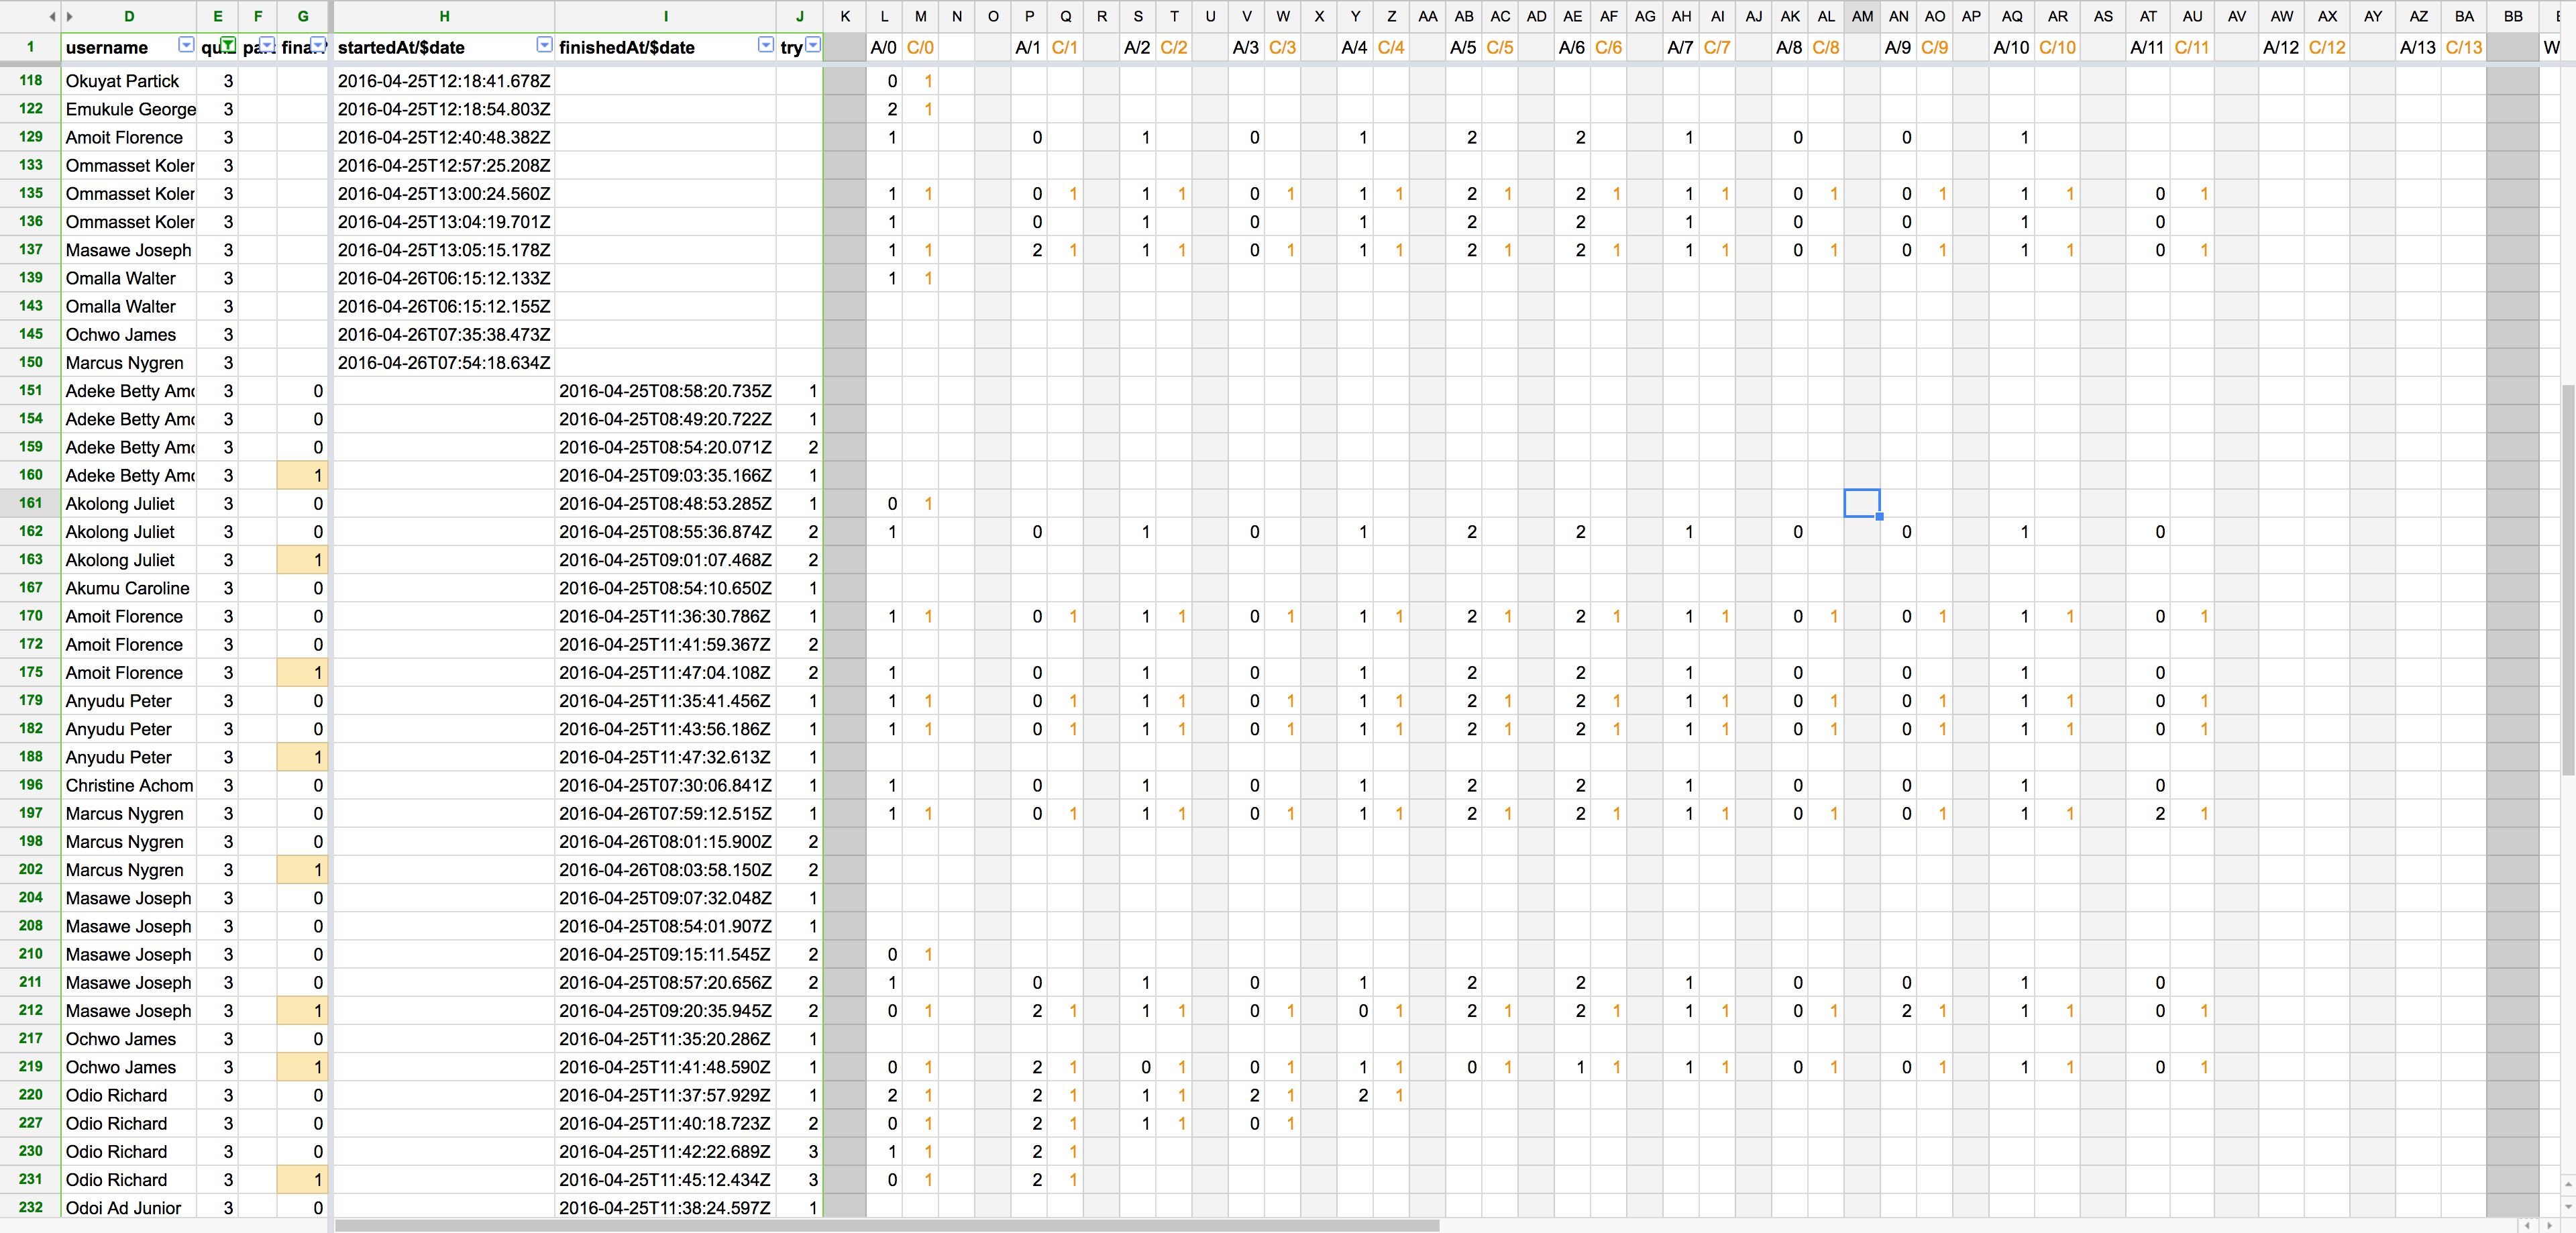
\includegraphics[width=0.9\textwidth]{analysis/resultsColored.png}
    \caption{The quiz results collected in a Google Sheet after data enhancement. In this figure, cell E1 has been filtered so that only results for quiz 3 are shown. Conditional formatting has been done with row G so that if it is a certification quiz, yellow color is used.}
    \label{fig:resultsColored}
\end{figure}

To be able to compare the test results with the pre-test results, it was clear that it would not be viable to test every dimension against every dimension. Instead, since goals of the app evaluation had been predefined in the following way, the quiz results were summarized into a new sheet so that the following could be derived:

\begin{itemize}
\item \% correct 1st try
\item number of tries until 100\%
\item number of tries until 100\% in 1 try
\end{itemize}

These could be calculated by having columns for:

\begin{itemize}
  \item Quiz 3
  \begin{itemize}
    \item Start time training
    \item \% correct 1st try
    \item number of tries until 100\% in 1 try
    \item Time difference start to end time certification
  \end{itemize}
  \item Quiz 9
  \begin{itemize}
    \item Start time training
    \item \% correct 1st try
    \item Time difference start to end 1st try
    \item Time difference start to passed training
    \item Time difference 1st try to certified
  \end{itemize}
\end{itemize}

Then, to see trends, color scales were again added. With ordinal values, a sequential color scheme is used (for example fastest time, from green to red), and with nominal values (like if they are female or male) where there is no right value, a qualitative color scheme is used. Now it was easier to spot outliers and trends, and giving validation to findings from notes and observations made during interviews, workshops and app tests.

\subsubsection{Step 4: Date Enhancement of Pre-study Results}
To see differences in answers more clearly, the data from the pre-study was made sortable and filterable. Then, the data was resampled for each column that had numerable (sortable) data in text instead of numbers, so for example "The day before" was changed to -1 and "The same day" to 0. In a similar way, school level was divided into four different groups, from 0 to 3, where 0 meant secondary, year unknown, 1 meant lower secondary, 2 meant upper secondary, and 3 meant tertiary.

After this, each column was given conditional formats using a color scale, using Google Sheets built-in functionality. This gave a visual way to quickly get an overview of the pre-test data.

\subsubsection{Step 5: Data Enhancement by Joining Pre-test and Results Summary}

The summary sheet and the pre-quiz sheet were joined, becoming a multiple-variate data set (several dimensions that were to bee compared with several other dimensions), see figure \ref{fig:analysFarg3}. A meeting with the university supervisors was held, so they could further give support in how to properly analyse the data. Since the two control groups showed similar means on the pre-quiz results, the two control groups were determined comparable.

\begin{figure}[h]
    \centering
    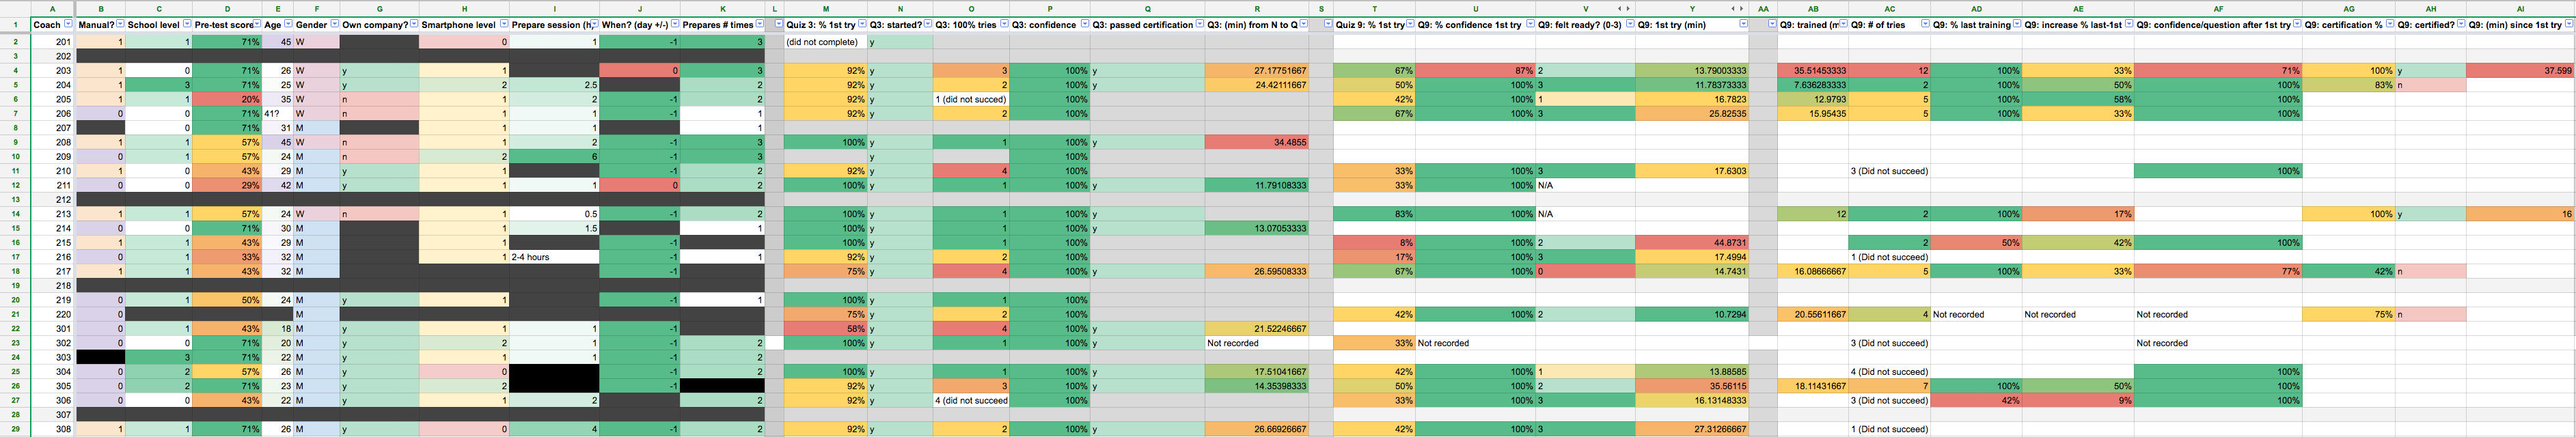
\includegraphics[width=1.0\textwidth]{analysis/sheets/0Overview.png}
    \caption{The multi-variate data set, made filterable and sortable in Google Sheets. Color scales and calculating means makes it easier to compare characteristics of the coach together with pre-test and quiz results. However, it is cumbersome and hard to quickly filter data on multiple parameters.}.
    \label{fig:analysFarg3}
\end{figure}

To meet the challenges of using Google Sheets, a multivariate analyzation software or a visualization was suggested to discover the data in less time. It was hard to determine a suitable multivariate analysis software suitable when having so few data points. Principle Component Analysis or Cohen's kappa would not be suitable, neither was it believed applicable to do Linear correlation on all dimensions. After discussion with other Master thesis students working with analysing data from various disciplines, parallel coordinates was suggested. It would allow very quickly filtering of the data, finding correlations, and distinguish outliers and common characteristics.

To guide the usage of the parallel coordinates (as there is so much to discover in the data set), using R to do Logistic correlation was also done. A disadvantage with this method, is that to be statistically significant, many data points may be needed, and it was now known before-hand if the method would be useful. Probably, parallel coordinates would be the best method to analyse a small multi-variate data set.

\subsubsection{Step 6: Visualization Mapping}
The goal with visualization mapping is to generate renderable data, in this case for the parallel coordinates visualization. Thus, a new spreadsheet is added, specific for visualizing the data. Columns were deleted that would serve no visual purpose (for example timestamps), gave all cells data values (even N/A when undefined), deleting users that did not have data, and shortened the column names so they would fit on the screen. The data was then exported from the Google Sheet into CSV.

\subsubsection{Step 7: Rendering}

For rendering, the JavaScript library D3.js, \citep{d3} was chosen. It supports data-driven documents for visualizing data with HTML, SVG and CSS. It supports both JSON and CSV data. A visual framework for multidimensional detectives for D3.js was found called "Parcoords.js", \cite{parcoords}. The example code from "Linking with a Data Table" provided the basis for the rendering. It allowed observing both the parallel coordinates visualization and the table data from the Google Sheet simultaneously.
% https://syntagmatic.github.io/parallel-coordinates/
% Chang, K. (2012). Parallel Coordinates toolkit : Parcoords.js 0.1. Parallel Coordinates toolkit. Retrieved September 8, 2012, from http://syntagmatic.github.com/parallel-coordinates/
% Kosara, R. (2010, May 13). Parallel Coordinates. Eagereyes.org. Retrieved September 8, 2012, from http://eagereyes.org/techniques/parallel-coordinates
% Tricaud, S. (2008). Picviz: finding a needle in a haystack. Proceedings WASL, San Diego. Retrieved from http://www.usenix.org/events/wasl08/tech/full_papers/tricaud/tricaud.pdf

 %https://syntagmatic.github.io/parallel-coordinates/examples/table.html

To work, the example CSV file was replaced with the data from exporting the Google Sheets data. To benefit the visualization, also the colors were changed, and the toolkit's functionality to drag the axes titles around to reorder the dimensions was used, since the goal was to quickly compare and find correlations. The result is visible in \ref{fig:parallell-coordinates-1}.

\begin{figure}[h]
    \centering
    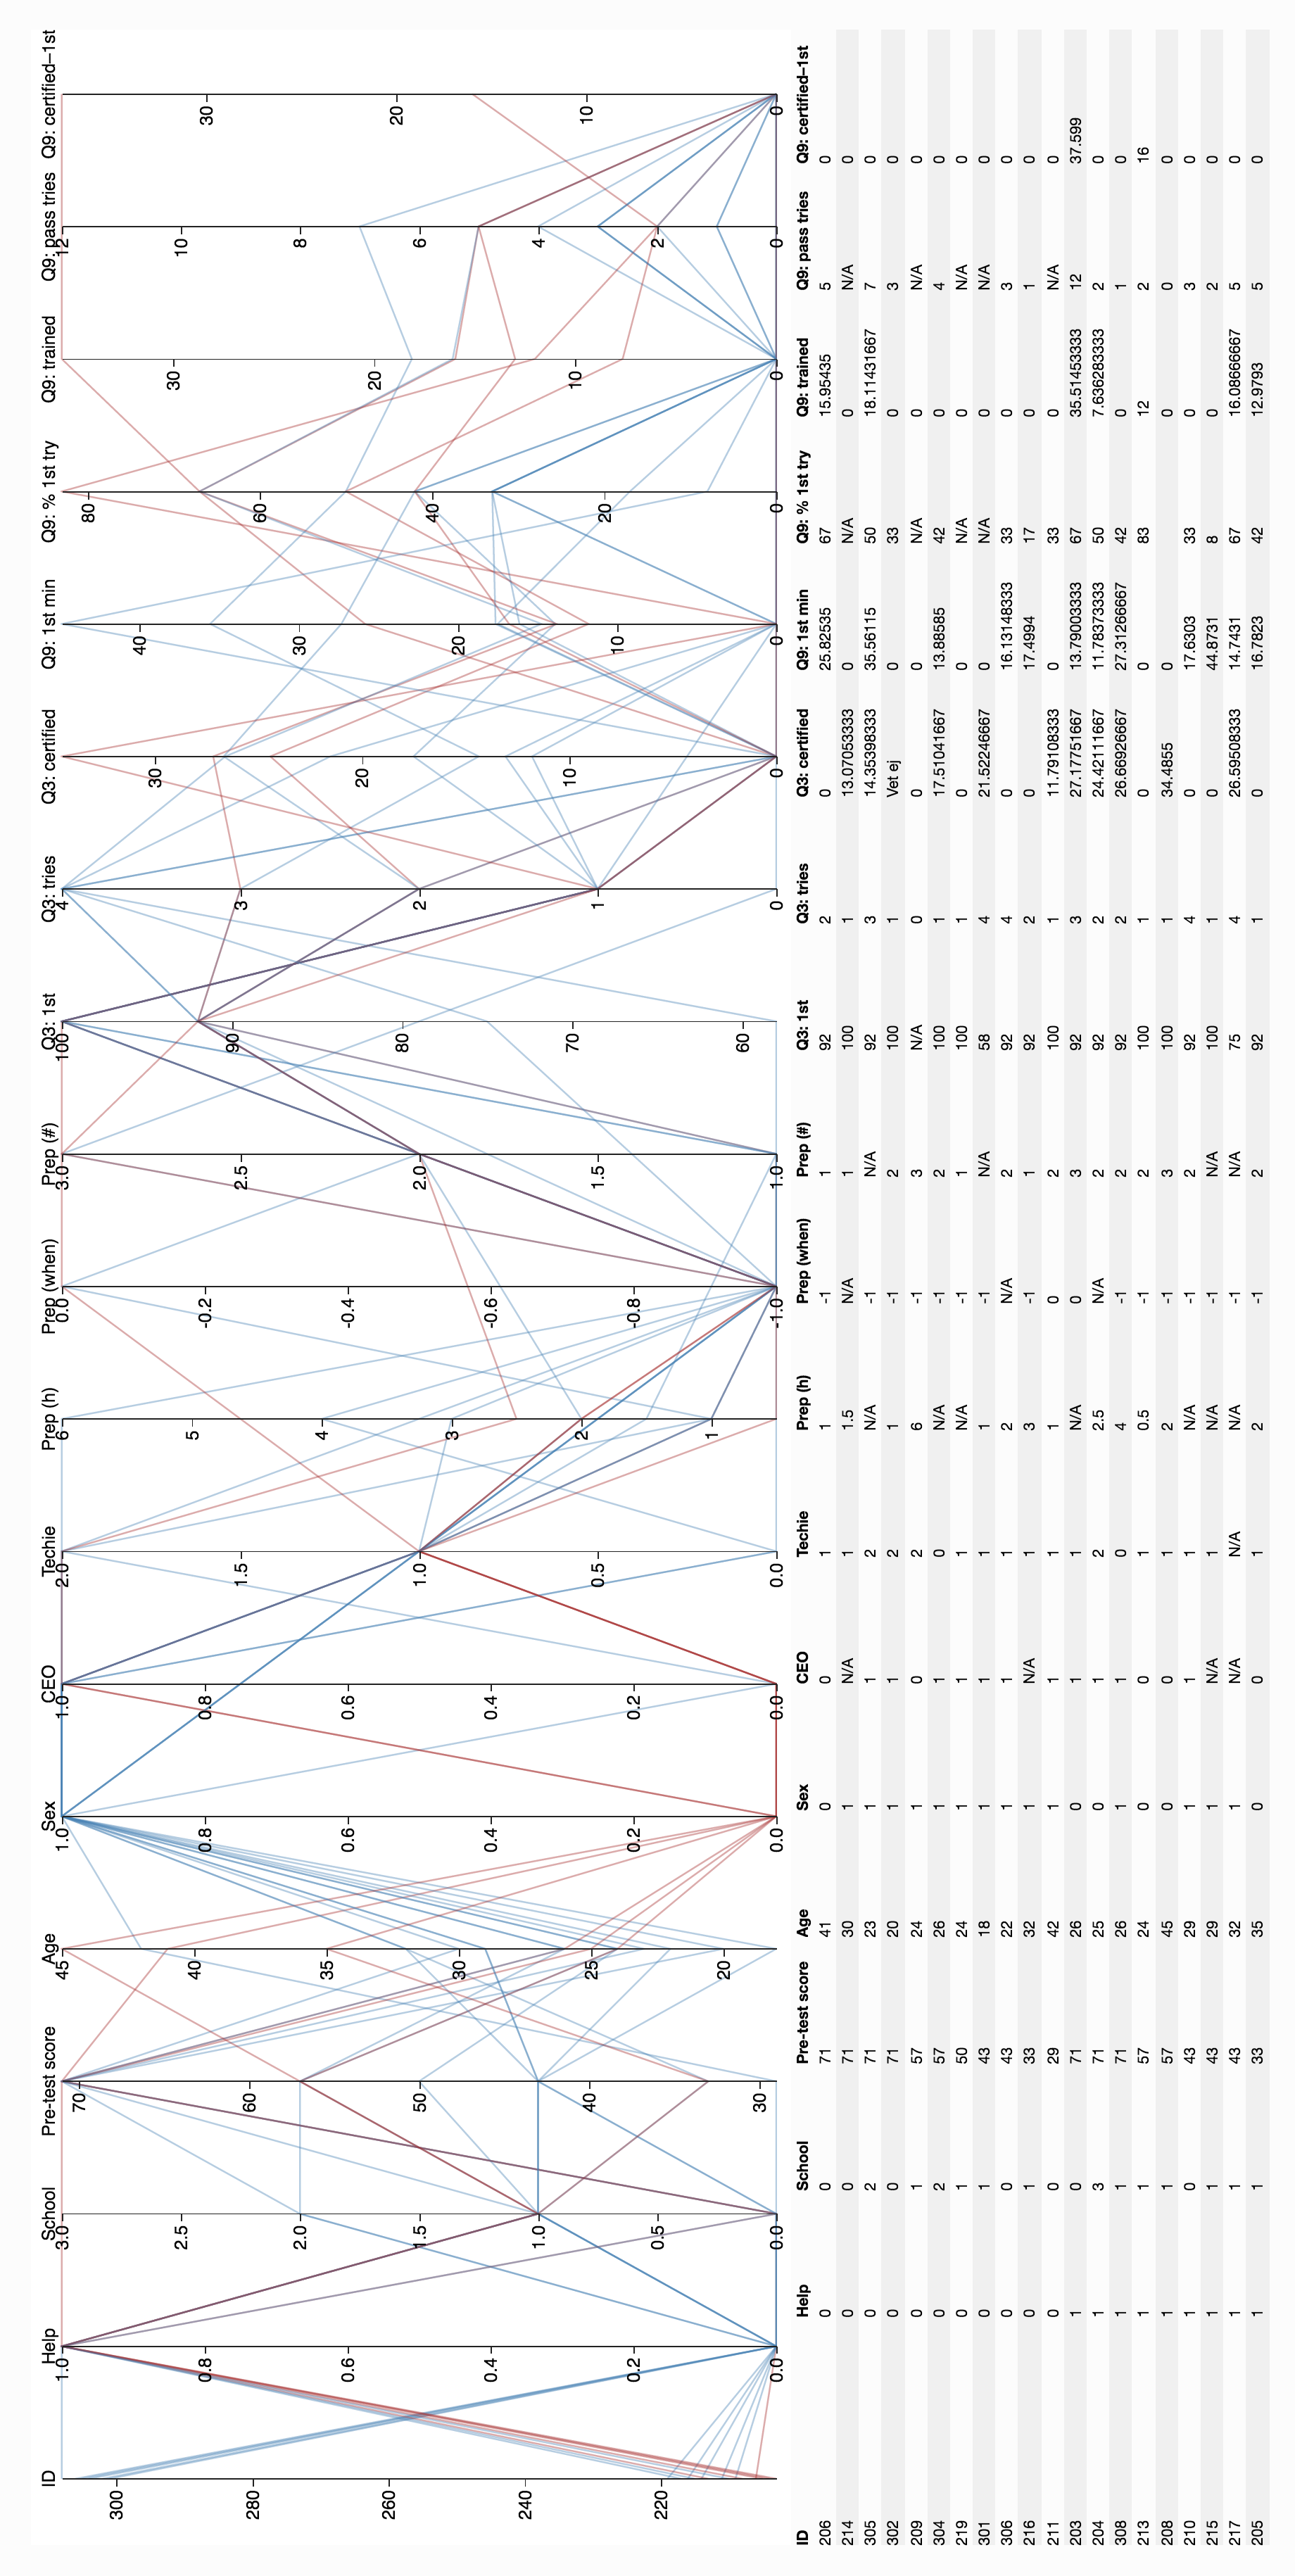
\includegraphics[width=0.7\textwidth]{analysis/parallellCoordinates3.png}
    \caption{The parallel coordinates visualization, done in d3.js. The visualization support draggable axes, filtering of data via dragging the sliders (which synchronizes with the data table), color assignment (like blue and red for men and women in the example), and hovering over a specific data point.}
    \label{fig:parallell-coordinates-1}
\end{figure}



\chapter{Results}\label{cha:Research}
%

% Ska följa som ett naturligt komplement till huvuddelen

In this chapter, the results are presented, so that in the next chapter, these results are analysed. %\todo{Flytta Insights som besvarar en Research Question till Discussion, och hänvisa till iteration. I Resultat vill vi bara ha Resultat, ej svar på forskningsfrågor, så spara svar på forskningsfrågor tills Diskussion.}

%\section{Example}\label{sec:research:history}
%
Liksom \citep{Duck:2005} har vi kommit fram till att glass smakar bäst på sommaren \citep{Khalil02NonlinearSystemsBook}.

\marginpar{Kommer att tänka på en liten anekdot\ldots}

\Warning[TODO]{Ta bort den löjliga anekdoten!}

\begin{figure}[tbp]
  \centering
  \subfloat[Alldeles för tidigt.][\label{fig:times:very-early}Det här är väl tidigt — din glass hinner smälta innan ditt sällskap dyker upp.]{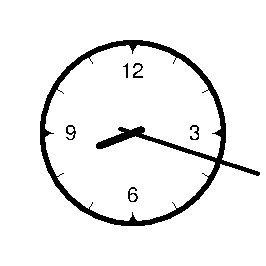
\includegraphics[page=1]{clocks}}
  \qquad
  \subfloat[Med marginal.][\label{fig:times:early}Kiosken stänger snart, men inte nu — perfekt!]{\includegraphics[page=2]{clocks}}
  \\
  \subfloat[I grevens tid.][\label{fig:times:on-time}Precis i tid — du får in ett finger i luckan just när kiosken ska stänga.  Han som jobbar blir sur, och det blir smolk i bägaren.]{\includegraphics[page=3]{clocks}}
  \qquad
  \subfloat[Försent.][\label{fig:times:late}Du är sen — kiosken är stängd.]{\includegraphics[page=4]{clocks}}
  \caption{\label{fig:times}%
    Illustration av \emph{subfloats}.  Den så kallade \emph{bounding box}en visas i \protect\subref{fig:times:late}.  Lägg märke till att bounding boxen har satts så att alla bilder har samma storlek, med enhetlig placering av själva innehållet i förhållande till bounding boxen.  Antag att du ska träffa en kompis för att äta glass just när kiosken stänger för dagen vid 08:30.  När dyker du upp?}
\end{figure}

\section{Developed Application}\label{developed-application}

  After three months time, the app developed has been successful in addressing YoungDrive's goals with the app, with very high precision to the needs and context of the end users. In figure~\ref{fig:iteration-map} the app development from iteration 1-4 are shown. The final app works on web or as an app, online or offline, on all of YoungDrive's Android and iOS devices. The app is fast to use, the back button on the phone can be used to go to the previous view, and the font size and images are consistent for each screen (which was not the case iteration 1-3, see figure \ref{fig:iteration-map} E-3. The goal was to provide a great learning experience, with a strong YoungDrive feel (embracing the values of fun, plus using the YoungDrive logo and colors).

  \todo{Flytta bild till helsida!}
  \begin{figure}[h]
    \centering
    \includegraphics[width=1.0\textwidth]{IterationMapLowRes.png}
    \caption{The app flow described as a timeline (A-I), per iteration (1-4). E.g. in iteration 4, login (B4) appears after choosing quiz to take (A4).}
    \label{fig:iteration-map}
  \end{figure}

  %\subsection{Iteration \#1}

  There was no developed application at this point.

  Instead, two workshops were held, which together would inform the future development of an application.

  There were the findings from those two workshops:

  \subsubsection{Workshop \#1: Customer Journey Map: A day as a coach}

  \subsubsection{Workshop \#2: Quizical and Duolingo}



  The quiz flow during iteration 1-2 was a standard multiple-choice quiz game, designed for assessment, but not for learning. In a scoreboard, they could see which questions they were awarded points for and not, with a total score, see figure \ref{fig:iteration-map} H-1. In the end of iteration 2, whey were encouraged to go back to the start screen, to redo the same quiz again, or select a new one. 1 point is awarded for correct answers, whereas 0 points is given for incorrect answers.

  In iteration 3, feedback for self-reflection was introduced. The coach answers Yes or No on "Are you sure?" for each question (figure \ref{fig:iteration-map} C-3), with the aim of increasing meta-cognitive skills, and being able to give personalized feedback in the score board.

  Thanks to recording both if they were correct and confident, the app can give very precise learning feedback (e.g. showing that the coach answered alternative B with confidence, but showing that A was actually the correct alternative).

  In iteration 3-4, after observing their incorrect answers, and learning their correct ones (closely compare figure \ref{fig:iteration-map} D-3 and E-3), they could retake the wrong answers immediately.

  In iteration 3, the score board was simply showing each correct question with the answer the coach provided versus the correct one. After giving feedback, the coach can train, and improve on incorrect answers and guesses, and when being 100\% correct and confident, ideally take the whole quiz without faults.

  For iteration 4, the score board is more personal, encouraging the coach to reflect on her own learning process. The feedback is designed to give a self-confidence boost ("You were correct, and you were sure" or "You guessed, but you were correct. You can answer with confidence the next time"), unlearn knowledge ("You were incorrect, but you were sure"), or encourage studying more when unsure and wrong ("You were incorrect, and you were not sure").

  To discourage guessing during training, since iteration 3, the coach is shown number of tries on the quiz if they do not get 100\% in their first try (see the top bar of figure \ref{fig:iteration-map} E-3). For iteration 4, the coach will also get a minus point (-1) for answering incorrectly but confidently "Are you sure?": "Yes". If uncertain, the coach should answer "Are yo sure?": "No", and no penalty will be given. The coach will later recieve feedback, either "You can be confident next time" (if correct but unsure) or "How can you get these correct next time?" (if unsure and incorrect).

  The coach is encouraged to be well-prepared before trying again (either consulting the answers or the manuals). At 100\% correct answers, they can get certified, by getting the whole quiz correct without faults. Failing a question on the certification would show that they have not \textit{reliably} learned all the answers during the training. The more effort the coach has put into the training, the more likely the coach will be to pass the certification.

  %Lena Tibell menade vid förslaget att "Belöna inte hur snabbt %en elev går från att kunna till att inte kunna, för olika %människor lär sig olika snabbt". "Vad vi ville åstadkomma %med Antal försök var endast att undvika gissningarna".

   This certification quiz is the same as in training, but no longer do they need to answer "Are you sure?". If the coach can again get 100\% correct answers, without any faults, they have proved they are correct and confident with the topic they should teach the youth.

   If they fail a question, the score board will encourage more training and that they did not get certified, see figure \ref{fig:iteration-map} H-4. Since the coach did get 100\% correct in the training (maybe after a couple of tries) but not in the certification, the knowledge can be described as "Can do with effort". The coach can choose to take a new quiz, or take the same quiz from the beginning of the training.

   For passing the certification on the 1st, 2nd or 3rd time the coach is awarded a Gold, Silver or Bronze medal respectively (after certificate try 3, no medal is given, only the certificate). Compare figure \ref{fig:iteration-map} I-3 to I-4: for iteration 4, the "certificate" mentions the persons name and the topic certified in, which is a form of gamification in addition to the intrisic motivation of rewarding deliberate practice.


In the following sections, you can read more about what data guided the development of the final app, as well as the results from the final app evaluation.

\section{Iteration 1: Uganda Coach Visit}

Here the results from the qualitative and quantitative data for iteration 1 are shown, together with conclusions.

\subsection{Qualitative data}

Below, the most important results from the stakeholder and coach interviews are presented.

\subsubsection{Stakeholder interview findings: Entrepreneurship education considerations}
Through early interviews with YoungDrive staff, it is clear that YoungDrive's entrepreneurship education methodology goes hand in hand with the presented theory. It's mottos are: "Dream big, start small", "Learning by doing" and "We have fun!" \citep{youngdrive-manual}.

Both in regards to designing for the users and for the above reason, the app should be a complement to YoundDrive's existing training material and the structure of the program.

A challenging part of the work is that YoungDrive consists of both the practical skills of the entrepreneur, theoretical material of running a business, and an entrepreneurial mindset. Therefore, both how to assess knowledge, and build habits, needs to be examined.

As the stakeholder interviews answered "What's it like being a coach?", their perspectives could now be understood and summed into a early understanding of the coach situation. The stakeholder interviews heavily informed the Questionnaire guide, highlighting aspects that had previously not been taken into account.

\subsubsection{Coach interview findings: Teaching with confidence}

The purpose of the coach interviews was to understand "What's it like being a coach?", from the coaches own perspective. Thanks to having similar interviews with stakeholders, their views could be compared. Also, more detailed answers on background, desires, experience and situation could be provided.

 From the interviews it was understood that CBTs can be responsible for from 7 up to 12 different youth groups in different programs, and such a high number places huge demands on the CBT. Even if there are only 7 groups, being behind on schedule or not being confident, can be very demanding.

%\textbf{Stayover at Patrick:} På morgonen visade Patrick mig hur han jobbar med deras tomt, var det odlas ris, och andra råvaror, deras djur, deras story från Syd-Sudan, till Kampala, till hyddan här i Tororo, och hans värderingar.

%Efter en ungdomssession nästföljande dag besökte vi och hälsade kort på en av de 2 CBT:s vi har session med idag. Sedan hade jag och Patrick den obligatoriska review av ungdoms-sessionen, och jag bjöd honom på middag. Kl. 19 ringde hans fru (som har börjat få tecken av malaria) och skyndade hem.

%Nästa ungdomssession fick jag besöka en annan CBT. Vi var tidiga. Sedan började jag prata med henne, och fick bra tillfälle att intervjua henne och även förklara för henne vad jag gjorde där. Det blev underligt att förklara för henne: Patrick påminde, när jag tabbat mig, att “Marcus, du måste förklara för X vad en app är”. Så hon fick låna min mobil, och jag förklarade att app var kort för applikation, och att för varje applikation har ett eget syfte, t.ex. ta foton. Jag bad henne klicka, svårt, råkade klicka åt henne, men sedan lät jag henne göra. Efter hon sett att det hon såg i skärmen var det hon såg på riktigt, blev hon jätteglad och började fundera vad hon skulle fota. Hon reste sig och gick runt hörnet, och jag följde efter. Hon fotade, efter att noggrannt tänkt igenom, att hon fotade buskarna med frukt. Sedan sade jag hon kunde fortsätta fota, och då tog hon ett litet runt hus utanför.

The interviews with CBTs, Project Leaders and stakeholders led to the realization that different coaches handles this differently well. All coaches possess high self-confidence in varying degrees in various situations, and as a result, quality among coaches is unbalanced, which they see as a challenge. Depending on the situation, everything is going according to plan, you are not confident, or you are falling behind with the schedule, you can be in one of these three Need groups:

\begin{itemize}
  \item The ideal coach
  \item The realistic coach
  \item The challenged coach
\end{itemize}

It was discovered that coach confidence comes largely from being able to have good youth sessions. This is important, because according to the interviews, being a high-quality YoungDrive coach to a large extent means having high-quality youth sessions. For having a high-quality youth session, these are the most important attributes:

\begin{itemize}
  \item Correct information
  \item Correct structure
  \item Time management
  \item Fun atmosphere
\end{itemize}

These findings were used to inform the Customer Journey Map workshop. In addition to the findings here, questions were also asked around etnography.


\subsection{Co-Creation Workshops}

    %What the data said

    Two workshops were held, which together would inform future development of an application. These were the findings from those two workshops:

    \subsubsection{Customer Journey Map: "A Day As a Coach"}

    %After the 15 minute introduction, they started with 5 minutes + 10 minutes discussion mapping out Before, During, After for the ideal coach, John. Green postits were used.

    %Since it took too much time to do this for the other two personas, they were given 5 minutes to either use pink post-its for steps that a realistic coach would skip, and yellow notes that the coach would do differently. This worked well, and the results were discussed within the 5 minutes between the coaches, and explained during 5 minutes witth audio recording.

    %Since they were understandingly tired, they were given a 10 minute break, during which time they were asked to think about things that could go wrong for the sad/angry persona, Suzan. When I got back from the toilet, they had already started working! I took time of 5 minutes, and they walked through the concerns and it’s effects, just like they had did with the 2nd persona.

    The three coaches understood the concept of the workshop surprisingly effortlessly, although the concept of postits and Customer Journey Map and Personas were unfamiliar to them. Contributing to the energy, was probably that the timeline and personas were largely informed by their interview answers. The workshop gave great insights for understanding the coach situation and the coaches themselves, both observing their behaviour during the workshop and learning about all the unknown activities involved in being a coach.

    The first workshop was concluded with many important insights. Thanks to using Personas, it was discovered from the workshop that the difference between coaches and the quality of the youth training was more diverse than originally thought. This is especially true when the coaches prepares for their youth session, an activity which was regarded as important as the coach training, but where quality of preparations were very divergent. This could be a great opportunity for delivering the app's promise of distance learning (see section \ref{purpose}). The teacher Josefina in an after-interview commented that while she can influence the coach training by her physical presence, she currently has no influence or insight into how the coach prepares, more than the co-project leaders' reports. When preparing for a session, there is a wide variety of \textit{when} the planning happens, and how a coach judges what amount of preparation is enough.

    Most coaches plan their next session during the morning, or immediately after a session with their group. Since a coach has somewhere between 7-10 groups (some even more), and the youth groups are at different modules, there is a lot of knowledge for the coach to handle - not only theoretical knowledge, but also the struggles of the youth, assignment presentations, workshops to be facilitated, etcetera. It is easy for a coach not to do everything as planned or as specified in the manual. Most of the coaches are said to be motivated by the possibility of becoming a better coach.

    According to the workshop, most of the coaches assess if they were ready for a topic \textit{after} a youth session. The feedback from the youth, as well as their questions and how well the coach can answer these, are the biggest informant. The exception is if the local project leaders comes to visit the youth session, but they do seldom have time to visit all of the coaches during a month, and during a month coaches should have taught 4 topics to all of their groups.

    \subsubsection{Smartphone Test using Quizoid and Duolingo}

    Quizoid (see figure \ref{fig:quizoid}) and Duolingo (see figure \ref{fig:duolingo}) were tested to understand the technical possibilities of the coaches, see figure \ref{fig:smartphoneTest}. They had circa 45 minutes to spend in each app, with discussions after each app test. The result was that the app can place itself somewhere in the middle of the two, regarding difficulty level.

    \begin{figure}[h]
        \centering
        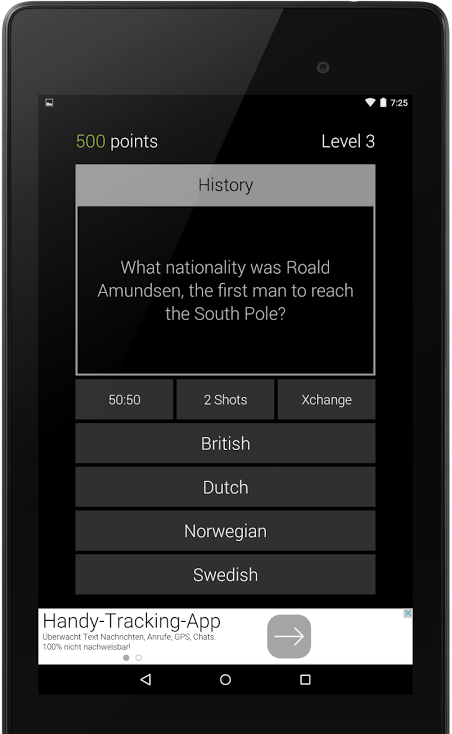
\includegraphics[width=0.5\textwidth]{quizoid.png}
        \caption{Quizoid is a simple multiple-choice game \citep{quizoid}, tested by coaches in iteration 1}.
        \label{fig:quizoid}
    \end{figure}

    \begin{figure}[h]
        \centering
        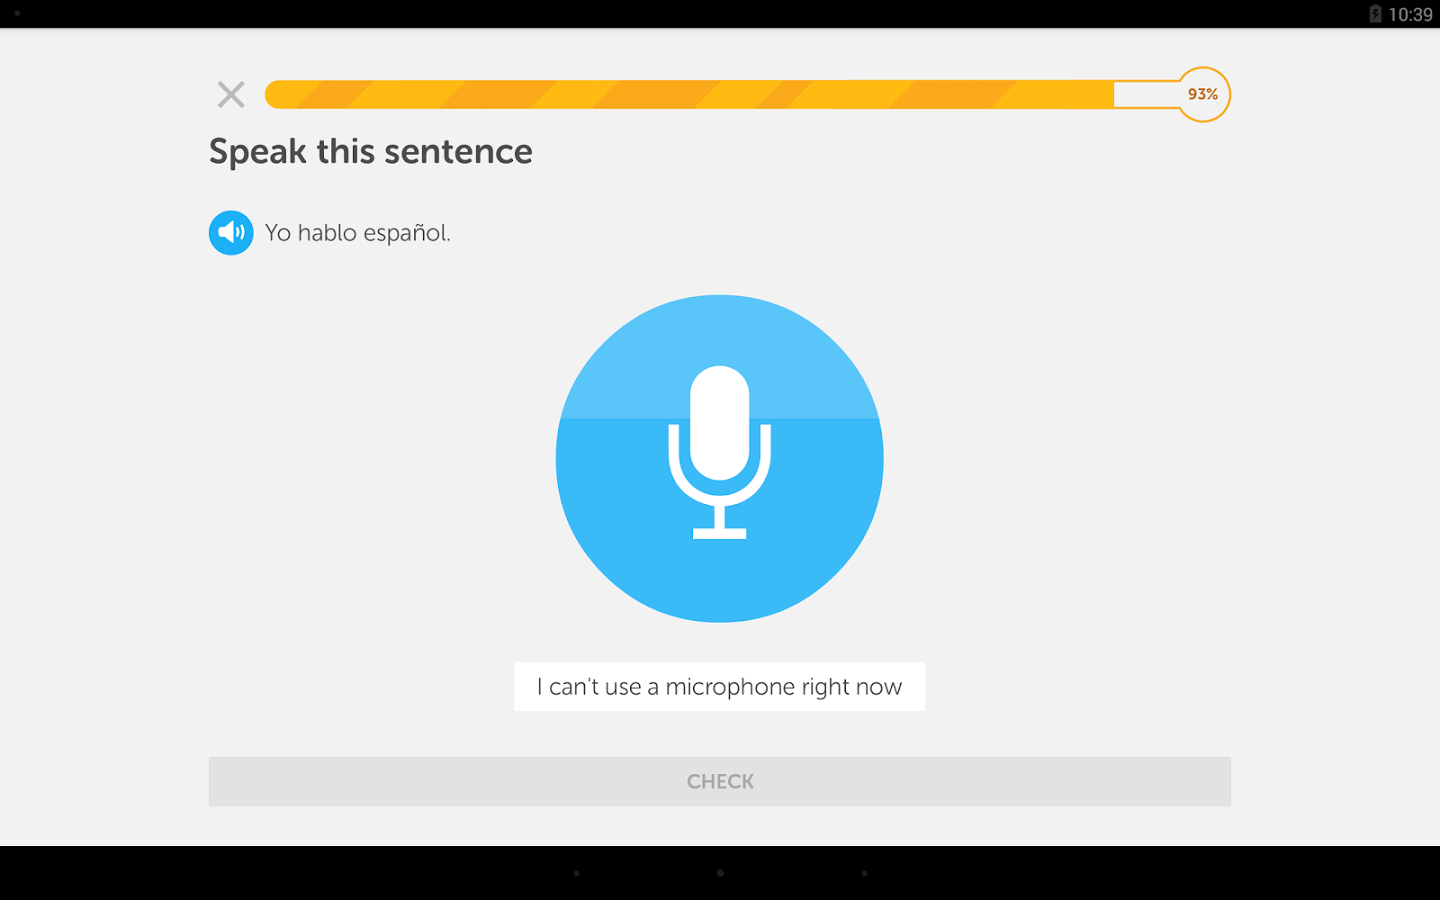
\includegraphics[width=0.7\textwidth]{duolingo.png}
        \caption{Duolingo is a praised app for language learning \citep{duolingo}, tested by coaches in iteration 1}.
        \label{fig:duolingo}
    \end{figure}

    \begin{figure}[h]
        \centering
        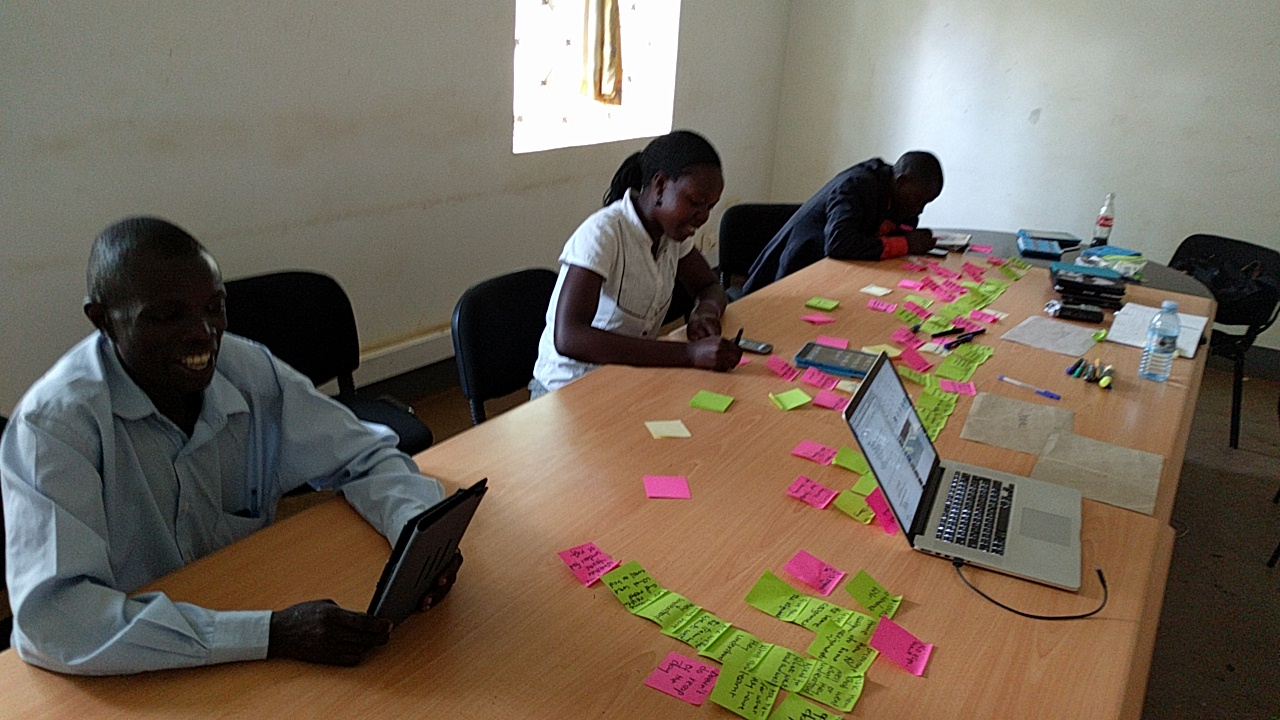
\includegraphics[width=0.7\textwidth]{iteration1/smartphoneTest.jpg}
        \caption{Picture from the smartphone test, observing how the coaches comprehend using Duolingo and Quizoid for the first time.}
        \label{fig:smartphoneTest}
    \end{figure}

    \clearpage

    Two of the three YoungDrive coaches (two of them being the local project leaders) used a smartphone for the first time. The attitude towards using a smartphone was overwhelmingly positive. One of the coaches even mentioned: "Marcus, today one of my dreams have gone true" regarding using a smartphone for the first time. He even asked if he could borrow one of the devices during the remainder of the stay. Even for coaches that had never touched a smartphone before, some concepts were easily understood (like using the camera and Quizoid).

    Other concepts were harder (accidently getting to the settings menu, unlocking the device, understanding advanced games, or training languages using Duolingo with advanced interactions). Point and click is easily understood, whereas sliding is much more unnatural.

\subsection{Discussion}

During a evaluation meeting with Linköping University and YoungDrive, it was determined that Iteration \#1 did provided answers for research question \#1, \#2, and \#3, and partly \#5. Thus, the iteration could be considered very successful, and now, the development of the app could begin.

It is clear from the data that the motivation of the app should be to assess and strengthen the entrepreneurship knowledge and skills of the coach. For coach quality to improve was a desire from the stakeholders as well as the coaches themselves, even if they were also satisfied with the current results. This lead to a challenging situation how an app can address becoming a better-performing coach.

An app could increase accuracy of correct information. With an app, the coach could keep a record of the module content, and see when and if they do need to refresh their skills. It was discovered that a coach app can benefit not only the coach training, but also in a surprisingly precise way, what was called "distance learning" in section \ref{purpose}. Accountability if the coach is ready for a session by automatic assessment. A very important aspect to increase learning and confidence will be to give good feedback (see section \ref{learning-assessment}).

With all the possible benefits of an app, it is definitely a problem that so few coaches have smartphones. Either continued development could be guided solely by the use case of having an app tailored for the coach training (where donated devices are available). But this would be to ignore that an app helping the coach to prepare for a session would be extremely beneficial, which discovered during the field visits to youth sessions and during interviews.

The motivation for using technology is very high, so one way forward would be that the app for distance training will reach only the users that can be given access to a smartphone, counting that more coaches will get smartphones in the future. Not using smartphones but feature phones (which all coaches possess), would mean building an SMS-based service (see \ref{rq1}.

As most coaches are already motivated to become a better coach and using technology, Sierra's \citep{sierra} advise of designing for their compelling context can be followed. From a YoungDrive perspective, this might mean "Given a teaching situation among the youth group, a great coach can teach an entrepreneurship topic more consistent with what the coach material said". Their performance in the YoungDrive app could translate into: "Given a question in the app, a great coach will get the right answer more often, and increasingly leverage the correct answer to their coach situation".

\subsection{Next iteration}
It is agreed with Josefina that the most important found skill of a YoungDrive coach is having great youth sessions. It is a challenge that the coach surely needs to feel, but does not always possess, self-confidence for its youth session. This partly stems from the lack of practical experience being put into realistic situations during the coach training.

If self-confidence comes from being able to deliver Correct Information, Correct Structure, Time Management and Fun Atmosphere, an app strengthening these will surely improve youth session quality. According to Josefina, assessing and increasing Correct Information is the parameter she values the most highly, and this will be the continued primary focus of the master thesis.

It is agreed with Josefina that preparing for a youth session can have an increased focus. It is a worry that designing for both the coach training and preparing for a session might be too ambitious within the given time frame. If so, designing for the coach training is deemed more important.


\section{Iteration 2: Zambia Coach Training}

Here the results from the qualitative and quantitative data for iteration 2 are shown, together with conclusions.

\subsection{Qualitative data}

\subsubsection{Design workshop \#1 in Zambia}

The result was fantastic, in the sense that it gave me an unbiased look at what the coaches expected from the app, what functionality wasn't important, and into their technical preferences.

The designs and insights gained were used throughout the week to further improve the app I had actually started creating, and gave great insights to who the coaches were and their thinking. \todo{Add image here}

\subsubsection{The desire perspective}

Insight: "The app could be used on my spare time". This is particularly true, about the bonus quizzes that were produced during the week.

Insight: \textit{Coach:} "I'll buy one" (a smartphone), \textit{Response from other coaches: } "Whoa!"

\subsubsection{The utility perspective}

Ideation: "The app should have notes, not only quesitions"

\subsubsection{The usability perspective}

Low resolution screens, made the text be barely visible. This showed, that the app needed to be tested on a lot of different devices. This is particularly true, as on day 1, the coaches did not know how to zoom, which could cause accident refreshs, frustration or confusion.

The app needs to work offline! To be online on the phone is too expensive for the coaches, and too unrealiable to give a satisfactory experience. Also, during testing, relying on internet can cause a lot of problems, especially if the teacher is alone.

\subsubsection{The learning perspective}

    The coaches had surprisingly high results, and at day 3 they wished harder questions when asked.

    We responded by having harder questions, e.g. by introducing similar answers, and testing 4 alternatives instead of 3. This was appreciated.

    The following analysis could be done:

    \subsubsection{Doing a pre-quiz: good for learning}
    When asked about what they thought about doing "Graduation" as a pre-quiz (before the session), 10/10 said they liked doing the quiz before, and that it benefited their learning during the session.

    When asked why it helped, these were the results:

    \begin{itemize}
    \item "During session, it is easier to follow" - 10 (100\%)
    \item "Giving the paper manuals before, scanning headings and pictures etc, would not help" - 10 (100\%)
    \end{itemize}

    It was also tested to work in group or individually. The ones who answered, said that you learned more individually (3/3), and more fun doing it together (3/3). Doing it together, was enjoyable as it was "Very easy because of using different minds" and "We can collaborate to do better".

    \subsubsection{Doing a post-quiz: Spaced versus massed learning}
    In "Goal setting", quotes were "I thought it was fun and challenging to do the quiz immediately afterwards", with another coach commenting "The mind was still fresh".

    When asked on timing preference, 10/10 said it would be more fun to do the quiz immediately afterwards, not at the end of the day. The motivation, seemed to be that it was easier.

    9/10, said they wanted to do the quiz afterwards. The outlier, said it would be better for learning doing it later.

    After this comment, this was the distribution:

    \begin{itemize}
    \item 3/10 wants to do the quiz both before and after a session
    \item 1/10 wants to do the quiz before and at the end of the day
    \item 7/10 wants to do the quiz only immediately afterwards
    \item 10/10 wants to do the quiz immediately afterwards, and then again at the end of the day
    \item 7/10 wants to do the quiz immediately afterwards, and then a joined quiz with other topics at the end of the day
    \end{itemize}

\subsubsection{The teacher perspective}

  \textbf{Low scores}
  The 9/19 shows the relevancy of the quiz, as Josefina did not think she would have discovered that the coach was lagging behind otherwise.

  In the data, it was observable that the coach had done well together with others, but 3/7 when done individually.

  Josefina said about the 9/19: "This is where a control group would be beneficial". "He is often passive during open questions, but active during the team exercises."

  The question we needed to ask ourselves, was: "Does this imply he is a good or bad coach?".

  \textbf{What would hinder Josefina from using the app}

  Josefina says: "Not doing data collection digitally works whenever they are 10 - but not with bigger numbers than that."

  According to the final interview with Josefina, she does not wish the app to replace her. She enjoys teaching, thinks she has an important role, and suggests the app to be designed to support her and the coaches, not replace her.

  \textbf{Acceptance criteria}

  If you have a high score, you are ready. If not, you need to redo the quiz.

  If you are 8/10 or lower, you are in the red zone. If lower than 10/10, they are not ready, the motivation being that what they don't know, they will teach in an improper way: affecting hundreds of youth. This is why Josefina thinks they should need all of the answers correct.

  \textbf{Testing Correct Structure, Time Management and Fun Atmosphere}
  Josefina informs that Correct Structure, Time Management and Fun Atmosphere would be the most valuable to test after a youth session. She also notes, that \textit{some} aseessment could be made via the app before a session. Because of the reason that this thesis does not focus on after-session-evaluation, Correct Information is primary to improving on the other factors, which are secondary.

\subsubsection{The developer perspective}

  \begin{itemize}
    \item Bugs was a big hindrance to functionality, and a lot (both high-dose, and high-scale) of testing is very important
    \item Simpler design than I thought (KISS) was sufficient
  \end{itemize}

\subsubsection{Bonus results: Testing the app on Kampala university student}
The app was tested on a university student from Makarere University.

The university student from Makarere University scored 100\% correct, in spite of not having any entrepreneurship training. This showed that guessing was possible, or that the quizzes were too easy.

\subsection{Quantitative Data}

    %What the data said

    This section presents the results from the two workshops held, in form of lessons learned. Also, some of the quiz results are shown.

    \subsubsection{Quiz Results from the Coaches}

    Quiz results ranges from the worst on 24\% (getting 4/17 correct answers) to 100\% (which has happened on 52/101 instances, for all of the quizzes). Week 9 was undoubtably the hardest quiz, with the topic being "Goal Setting and Action Plan" (17 questions, average being 76.22\% correct answers, 18 quiz results submitted). The easiest quizzes are week 3 "Financial literacy" (11 questions), week 6 "Mastering sales" (9 questions) and week 7 "Sales day" (3 questions), where all of the results are 100\%.

    There are some amount of coaches that have taken the same quizzes multiple times. From this, interesting conclusions can be drawn. Attending the lecture shows a 15.0\% average increase in quiz results, compared to an 12.8\% increase with simply taking the quiz two times. This shows that a lecture is still more effective than learning via the app.

    Time to finish a quiz took between 2 minutes to 33 minutes (3/4 quizzes that took longer than 25 minutes were on quiz 9, there is a correlation with number of questions). Most of the quizzes took under 5 minutes to complete, and results are always over 80\% for these instances. This shows that the coach had a high confidence with the answers. Similarly, all of the scores under 60\% has taken more than 20 minutes. This can be explained by that the coach is unfamiliar with the app or smartphone, and that the coach is uncertain of the answers.

    It is seen in the quiz results that the quizzes did get gradually more challenging, as the average of quiz scores gets lower after day 3 of training, when it was discovered was welcoming the quizzes to get harder.

    The quiz scores when quizzes are performed in group is very varying (from 24\% to 100\%), and it is observed that influence of another coach can lead both to a worse score than their individual average, and a higher score. It is interesting to see that the three coaches that have the worst average (67, 72 and 85\%) are also the ones that have taken quizzes the least times individually, and the most taking quizzes together with others. This may show that the app is more effective when used individually, and there seem no other connection to previous entrepreneurial activity or background.

    There are few correlations that can be made between the coach's background and experience, compared with quiz results or app behavior. Nothing in the coach information distinguishes the worst 3 performers in the quiz. For the opposite, there is however a noticable behaviour that being confident, having trained youth, leadership experience, business experience, care for community, care for oneself and confidence to take on many youth, almost guarantees a high quiz average (which demonstrates learning) and quizzes done (which demonstrates motivation).

    For coaches with 0-1 negative remarks during the interviews (n=6) compared to coaches with 2-4 negative remarks (n=4), their quiz average is but 2\% higher (87\% to 85\%). This is not significant, but this number is increased to 93\% (an 8\% increase) if the outlier from the group is removed (a coach which only did three quizzes with average of 57\%). In the future, more research could be done into comparing coach data with quiz results.

    %Comparing instances when coaches have taken a test before and after a lecture, the results are: 71\%to 100\%, 59\% to 74\%, 80\% to 86\%, 90\% to 100\%. Without the lecture, improvements has been from 80 to 90, 100 to 100 to 100, 90 to 90, 80 to 100, 90 to 100, 100 to 100, 86 to 100, 100 to 100, 90 to 100.

    \subsubsection{Lessons Learned from Unbiased App Design by Coaches: Use Case 1}

    The result was fantastic, in the sense that it gave an unbiased look at what the coaches expected from the app, what functionality wasn't important, and into their technical preferences. A simpler design than originally thought was deemed sufficient, and the simple sketches guided continued development of the app during the week. From using the devices, it was found that most coaches prefer using the tablet (5 for tablet, versus 2 for smartphone and 2 for computer). Both the designs and insights gained were used throughout the week to further improve the simple app created at the end of iteration 1. The workshop gave great insights to who the coaches were and their thinking. \todo{Add image here}

    \subsubsection{Lessons Learned from Unbiased App Design by Coaches: Use Case 2}

    During this workshop, the focus was to examine what builds confidence among the coaches. The following clusters could be determined: "I believe in myself" (3 coaches), "I believe in God" (2 coaches), "I am well prepared" (4 coaches) and "I am certified" (1 coach). See figure \ref{fig:zambiaWorkshop2} for the different clusters.

    \todo{Make full-page}
    \begin{figure}[h]
        \centering
        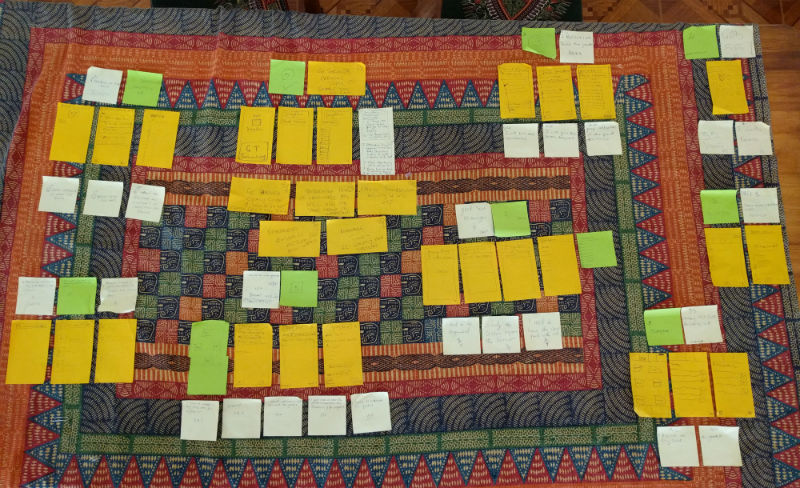
\includegraphics[width=0.7\textwidth]{zambiaWorkshop2small.jpg}
        \caption{The clustered postits with needs, together with included design proposals.}
        \label{fig:iteration}
    \end{figure}

    Josefina comments after the workshop: “I have a problem: There is no way I can control them how they have prepared themselves for a youth session.", says Josefina.

\subsection{Discussion}

The quantative and qualitative data from iteration 2 shows that the app works for "validating the coaches' level of knowledge during their education", which was the main purpose of the master thesis (see section \ref{rq}. Now, the app should be tested in Uganda as well, and there can be an increased focus on "distance training" and "certify all staff".

Iteration 2 has translated the theoretical understanding of answering research question 1, 2, 3 and 5 into practical experience. Now there are observable evidence for what the interactions from Iteration 1 showed:

\begin{itemize}
\item The purpose of the coach training should be to prepare the coach in having great youth sessions
\item Therefore, this is what the quizzess should assess
\item What it really means being a good YoungDrive coach, is having good youth sessions
\item
\end{itemize}

\subsubsection{Validating the coaches' level of knowledge}
The quiz results data shows that a lecture is still currently more valuable than taking a quiz in the app two times to improve (15.0\% to 12.8\%). For iteration 2, work on answering research question 4 has started. While the teacher has appreciated the multiple-choice assessment, challenges of designing test questions to support entrepreneurial learning has been found. It is clear that the app is valuable for assessment, increasing coach self-awareness and being a valuable indicator for the teacher. However, the questions formulated scores low on Bloom's revised taxonomy \cite{bloom} compared with YoungDrive's educational objectives for the topics.

There are previously found issues with using multiple-choice for assessment and learning, but they seem to become especially relevant in the context of teaching entrepreneurship.

Either question formulation needs to be improved, or creative design solutions needs to be experimented with which can increase coach understanding and identify and reduce guessing. This needs to be further investigated for iteration 3.

Test with university student scored 100\% correct, means that common sense can go a long way, and that the results can't be 100\% trustworthy, and that multiple-choice questions has serious issues - this, we already knew during and before the coach training - but it needs to be taken care of. Similarly business and leadership experience for the coach seems to lead to a higher quiz average, while a low quiz average can't seem to be relatable to any of the coach characteristics found during the interviews. This makes it hard to design the app for different types of coaches, without testing other parameters, which should be done in iteration 4 for the summative test.

\subsubsection{Distance learning}
In addition to the formative app tests, workshop \# 2 heavily informs what is necessary when designing for use case 2, distance learning: preparing a session in regards to building confidence. The results from the workshop are somewhat surprising, factors not only those that relate to the four parameters from iteration 1 ("I am well prepared" and "I believe in myself"), but for some also "I believe in God" or "I am certified" (which relates to purpose 3 of the app). These should be considered for iteration 3.

Further, app tests expose how the app is currently not actively designed with learning in mind, and thus not distance learning. This is unfortunate, both because distance learning is important, and as the app test with refugee innovators shows that there is an opportunity doing entrepreneurship training in rural areas outside of YoungDrive's coverage area. In order for online coach-training to work for distance learning, learning and feedback, and not only assessment, is however essential.

While it may be technically possible, the teacher desires the app support her during the coach training, not replace her. Therefore, completely replacing the teacher with an app should be avoided. The teacher is very important for giving coaching and educating in a way that the app can't. But the teacher can also be empowered by the app. For the future, Josefina would have liked to be able to stop coaches from having taught, if they do not have 90-100 \% correct information on the subject. Today, Josefina can not assess this. This means that some coaches, are teaching incorrect information to hundreds of youth. Here, the quiz has a very good need to fill.

If wrong on an answer, the app today has no means of giving high pay-off tips to get to 100\%, or exposing you to deliberate practice or perceptual exposure. If the coach gets 9/10 correct answers reliably, or gets 5/10 answers with guesses, the coach still needs to retake all answers, not having learned the correct answer before taking the quiz again.

How to develop the app to solve these issues, is not obvious. Multiple strategies could and should be used. The app could benefit from introducing smart feedback encouraging a growth mindset ("You did not get 100\% \textit{yet}") \cite{dweck}.

\subsection{Next iteration}
After the meeting with the partner and expert group, the following was concluded from iteration \#2:

\begin{itemize}
\item The app is partly working on assessment now, but not for learning. Are coaches really learning via the app, especially learning to be better coaches?
\begin{itemize}
  \item Multiple-choice is flawed in its current form. How can guesses be identified and reduced in a multiple-choice format? How can answering questions improve confidence and encourage learning?
  \item How can questions be formulated in a way that teaches entrepreneurship, which is so practical?
\end{itemize}
\item The need for a field app still feels relevant (especially for sessions long since the coach training)
  \begin{itemize}
  \item An app could be used, either before you start planning (to guide what you need to study the most on), or after you think you are ready (so you can assess and improve).
  \item When designing the app, it is concluded that an app for coach training, and an app to use before a youth session, should be able to be the same app if possible, since the purpose of preparing the coach to be great with its youth session is the same.
  \item Discussing the importance of self-reflection after a youth session with Josefina, led to asking more of such questions in coach quizzes. While Fun Atmosphere can be hard to assess using multiple-choice, can Correct Structure and Time Management be assessed?
  \end{itemize}
\end{itemize}

After the partner and expert meeting, it was decided that the following needs to be done for iteration 3:

\begin{itemize}
  \item Make sure that the coach actually learnes the desired educational objectives
  \begin{itemize}
    \item Create a new quiz guided by Josefina, "Are you ready for Session 9?", also to test if Correct Structure and Time Management could be assessed using multiple-choice
    \item See if design additions to multiple-choice can increase learning in-line with Bloom's revised taxonomy
  \end{itemize}
  \item Design quiz app for learning, focus on field app, and have a design that works stand-alone from the YoungDrive coach training in mind.
  \begin{itemize}
    \item Investigate the effect of giving growth mindset feedback in the app (The Power of Yet approach)
  \end{itemize}
  \item Test if the app created in Zambia could work also in Uganda
    \begin{itemize}
      \item This also means converting all the questions from the new (Zambia) manual to the old (Uganda) manual, since both structure and content of the manuals has changed.
    \end{itemize}

  \end{itemize}
\end{itemize}


\section{Iteration 3: Uganda Formative Test}

Here the results from the qualitative and quantitative data for iteration 3 are shown, together with conclusions.

For the coach training in iteration 1, only assessment was okay, since Josefina could give feedback. But if assessing preparedness for a youth session, the app leaving the coach with not being ready is not viable. Given a coach having prepared for their youth session on week 9, and then only scoring 5/10, what should happen? In a similar way, what should happen if 9/10 correct answers? Clearly, if the coach has 9/10, this coach should get feedback to improve, and especially if the score has been 5/10.

\subsection{Qualitative data}

  %What the observations said

  \subsubsection{Observations from Kampala test}
  The entrepreneurship student in Kampala, informed the following changes:

  Instead of "Become certified", he would be more motivated by unlocking the opportunity to apply the skills.

  "Improve" should be renamed "Try again", because it is more intuitive.

  His overall opinion on the app was:

  "Can you give me the link, because I'd love to do more of this. I think it's amazing."

  \subsubsection{Verified relevancy of seperating Training and Certification}
  When asked for an opinion, Josefina answered: "I like the idea that when the coaches have answered all of the questions correctly, they can consilidate the knowledge by the certification test, when the coach should get 100\% correct on their first try."

  \subsubsection{Field visits}

  The first thought was to use Gold/Silver/Bronze in the Training mode, and "Are you sure?" in the Certification mode. User tests showed that the other way around was better.

  \subsubsection{Big app test}
  \textbf{Learning: } The app test simulated the app being used to assess preparedness for a youth session. They clearly showed evidence between the difference between designing for Assessment and Learning:

  Given a coach having prepared for their youth session on week 9, and then only scoring 5/10, what should happen? In a similar way, what should happen if 9/10 correct answers?

  For the coach training, the assessment was okay, since Josefina could pick up and give feedback.

  Before a youth session, leaving the coach there is not viable. If the coach has 9/10, that coach should not only be let be, and especially if the score has been 5/10.

  Feedback was that one user did not want to press "Improve", until having read the manual. The motivation was: "Not because that is what the info says, but because I can learn more from the manual, about more than what the questions says."

  This is indeed the preferred behaviour from Josefina, and the app should continue to encourage only using the app training or certification mode after having prepared via the manual. This way, the app is still assessment, but it is "learning by thinking", with feedback.

    %What the data said

    \subsection{Big Formative App Test}
  The app test simulated the app being used to assess preparedness for a youth session. The test clearly showed evidence between the difference between designing for Assessment and Learning. See figure \ref{fig:tabletTest} and figure \ref{fig:computerTest} to understand the setting.

  Before the quiz started, the coaches were asked to raise their hand if they felt proficient with using a smart phone. 8 out of 23 said yes. After using the app, 16 thought they were proficient (25\% increase), while 5 said low proficiency, and 2 said no (we don't yet feel proficient, still fear).

  The test was done in pairs, because of lack of devices. Manual data collection of quiz results was not viable with coaches more than 10 people (as Josefina said in Zambia), it got to hectic, which is why not all quiz results were recorded, only when coaches raised their hands, which they often did only when they got 100\%, and some never raised their hand. The results gathered can be seen in figure \ref{fig:iteration3data}.

  A couple of notes can be made from the quantitative data. 6 groups consisted of two CBTs, and 5 groups were mixed (1 CBT and 1 Youth Mentor in the group). Among the CBT groups, the average score on a quiz was 77\%, while the presence of a Youth Mentor increased the average to 98\%. The groups were free to choose whichever quiz they wanted to. Only one group chose to redo the same quiz (scoring 100\% both times), while all others varied between different quizzes. Out of 18 quiz instances, 85\% was the mean (versus a 89\% average over 105 instances in Zambia), with 1 instance of 0\% (0/15!), 35\%, 53\%, 71\%, 2 instances of 83\%, and 12 instances of 100\%. The lower result than in Zambia could be that in Zambia the topics were still fresh, and that in Uganda, much of the information from the earlier topics of the training has not been repeated in a long time.

  \begin{figure}[h]
    \centering
    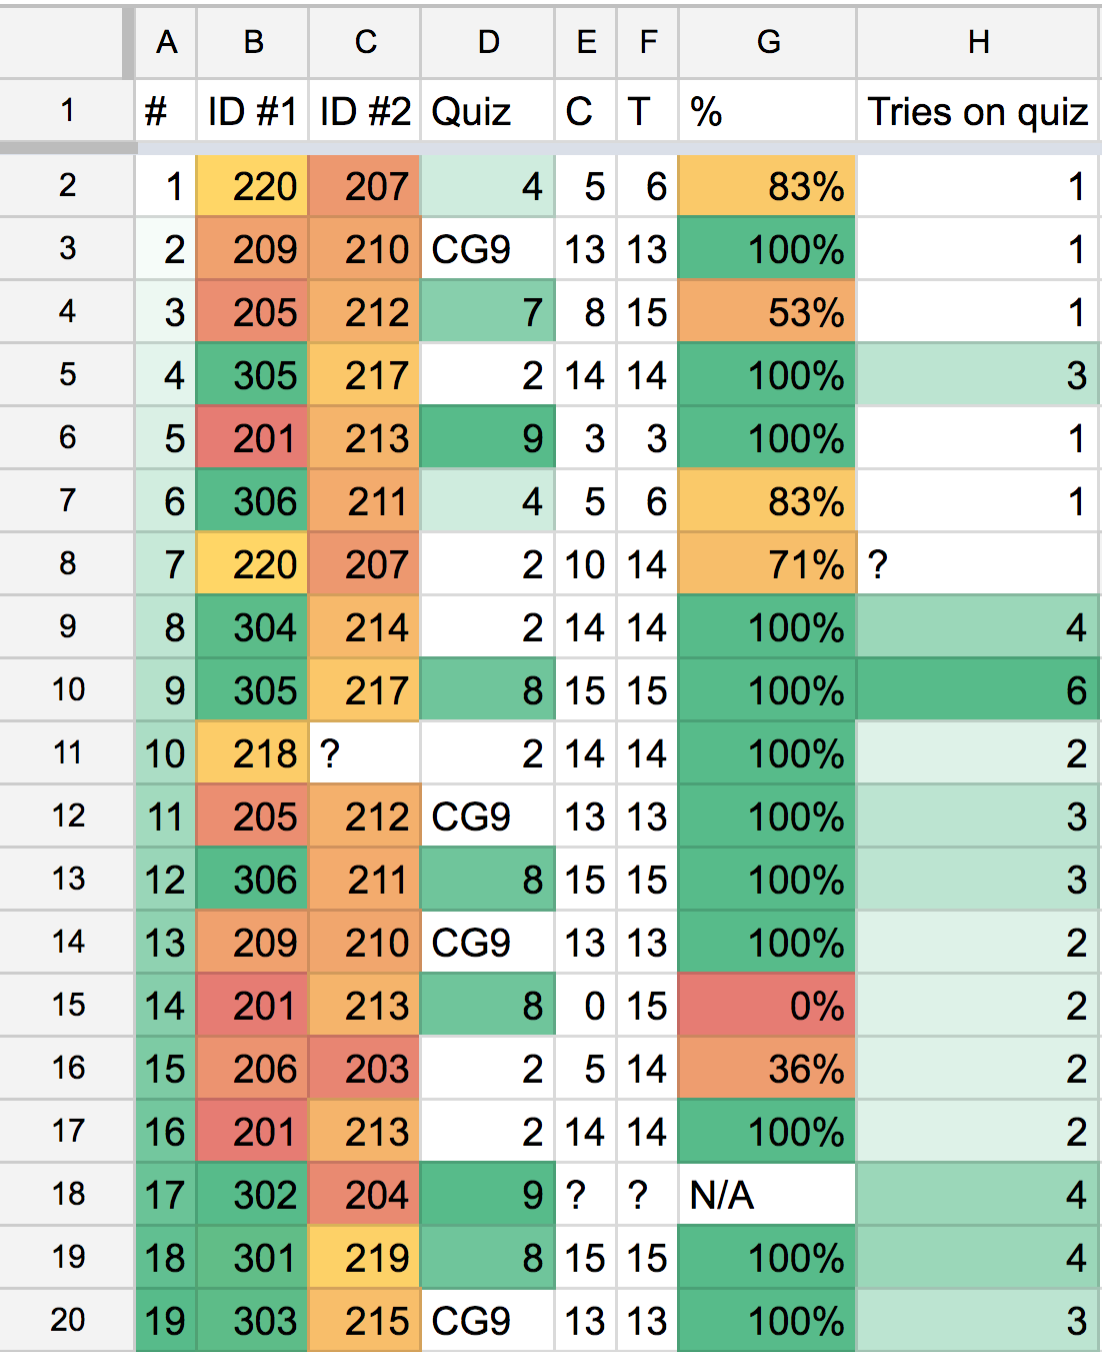
\includegraphics[width=0.8\textwidth]{analysis/iteration3data.png}
    \caption{The data gathered from iteration 3. A is order of quiz submission, B and C is Coach ID for coach 1 and 2 in the group, C is quiz chosen (CS9 meaning "Coach guide week 9"), D is correct answers, E is number of questions, G is percentage correct answers, and F is recorded quiz try on the particular topic at the time of submission.}
    \label{fig:iteration3data}
  \end{figure}

  An aspect which makes the data analysis less usable is that since the quizzes were carried out in pairs, the results are non-traceable to individuals, and pre-knowledge about the coaches or for iteration 4. This is why such a large focus has been on observations.

  \begin{figure}[h]
    \centering
    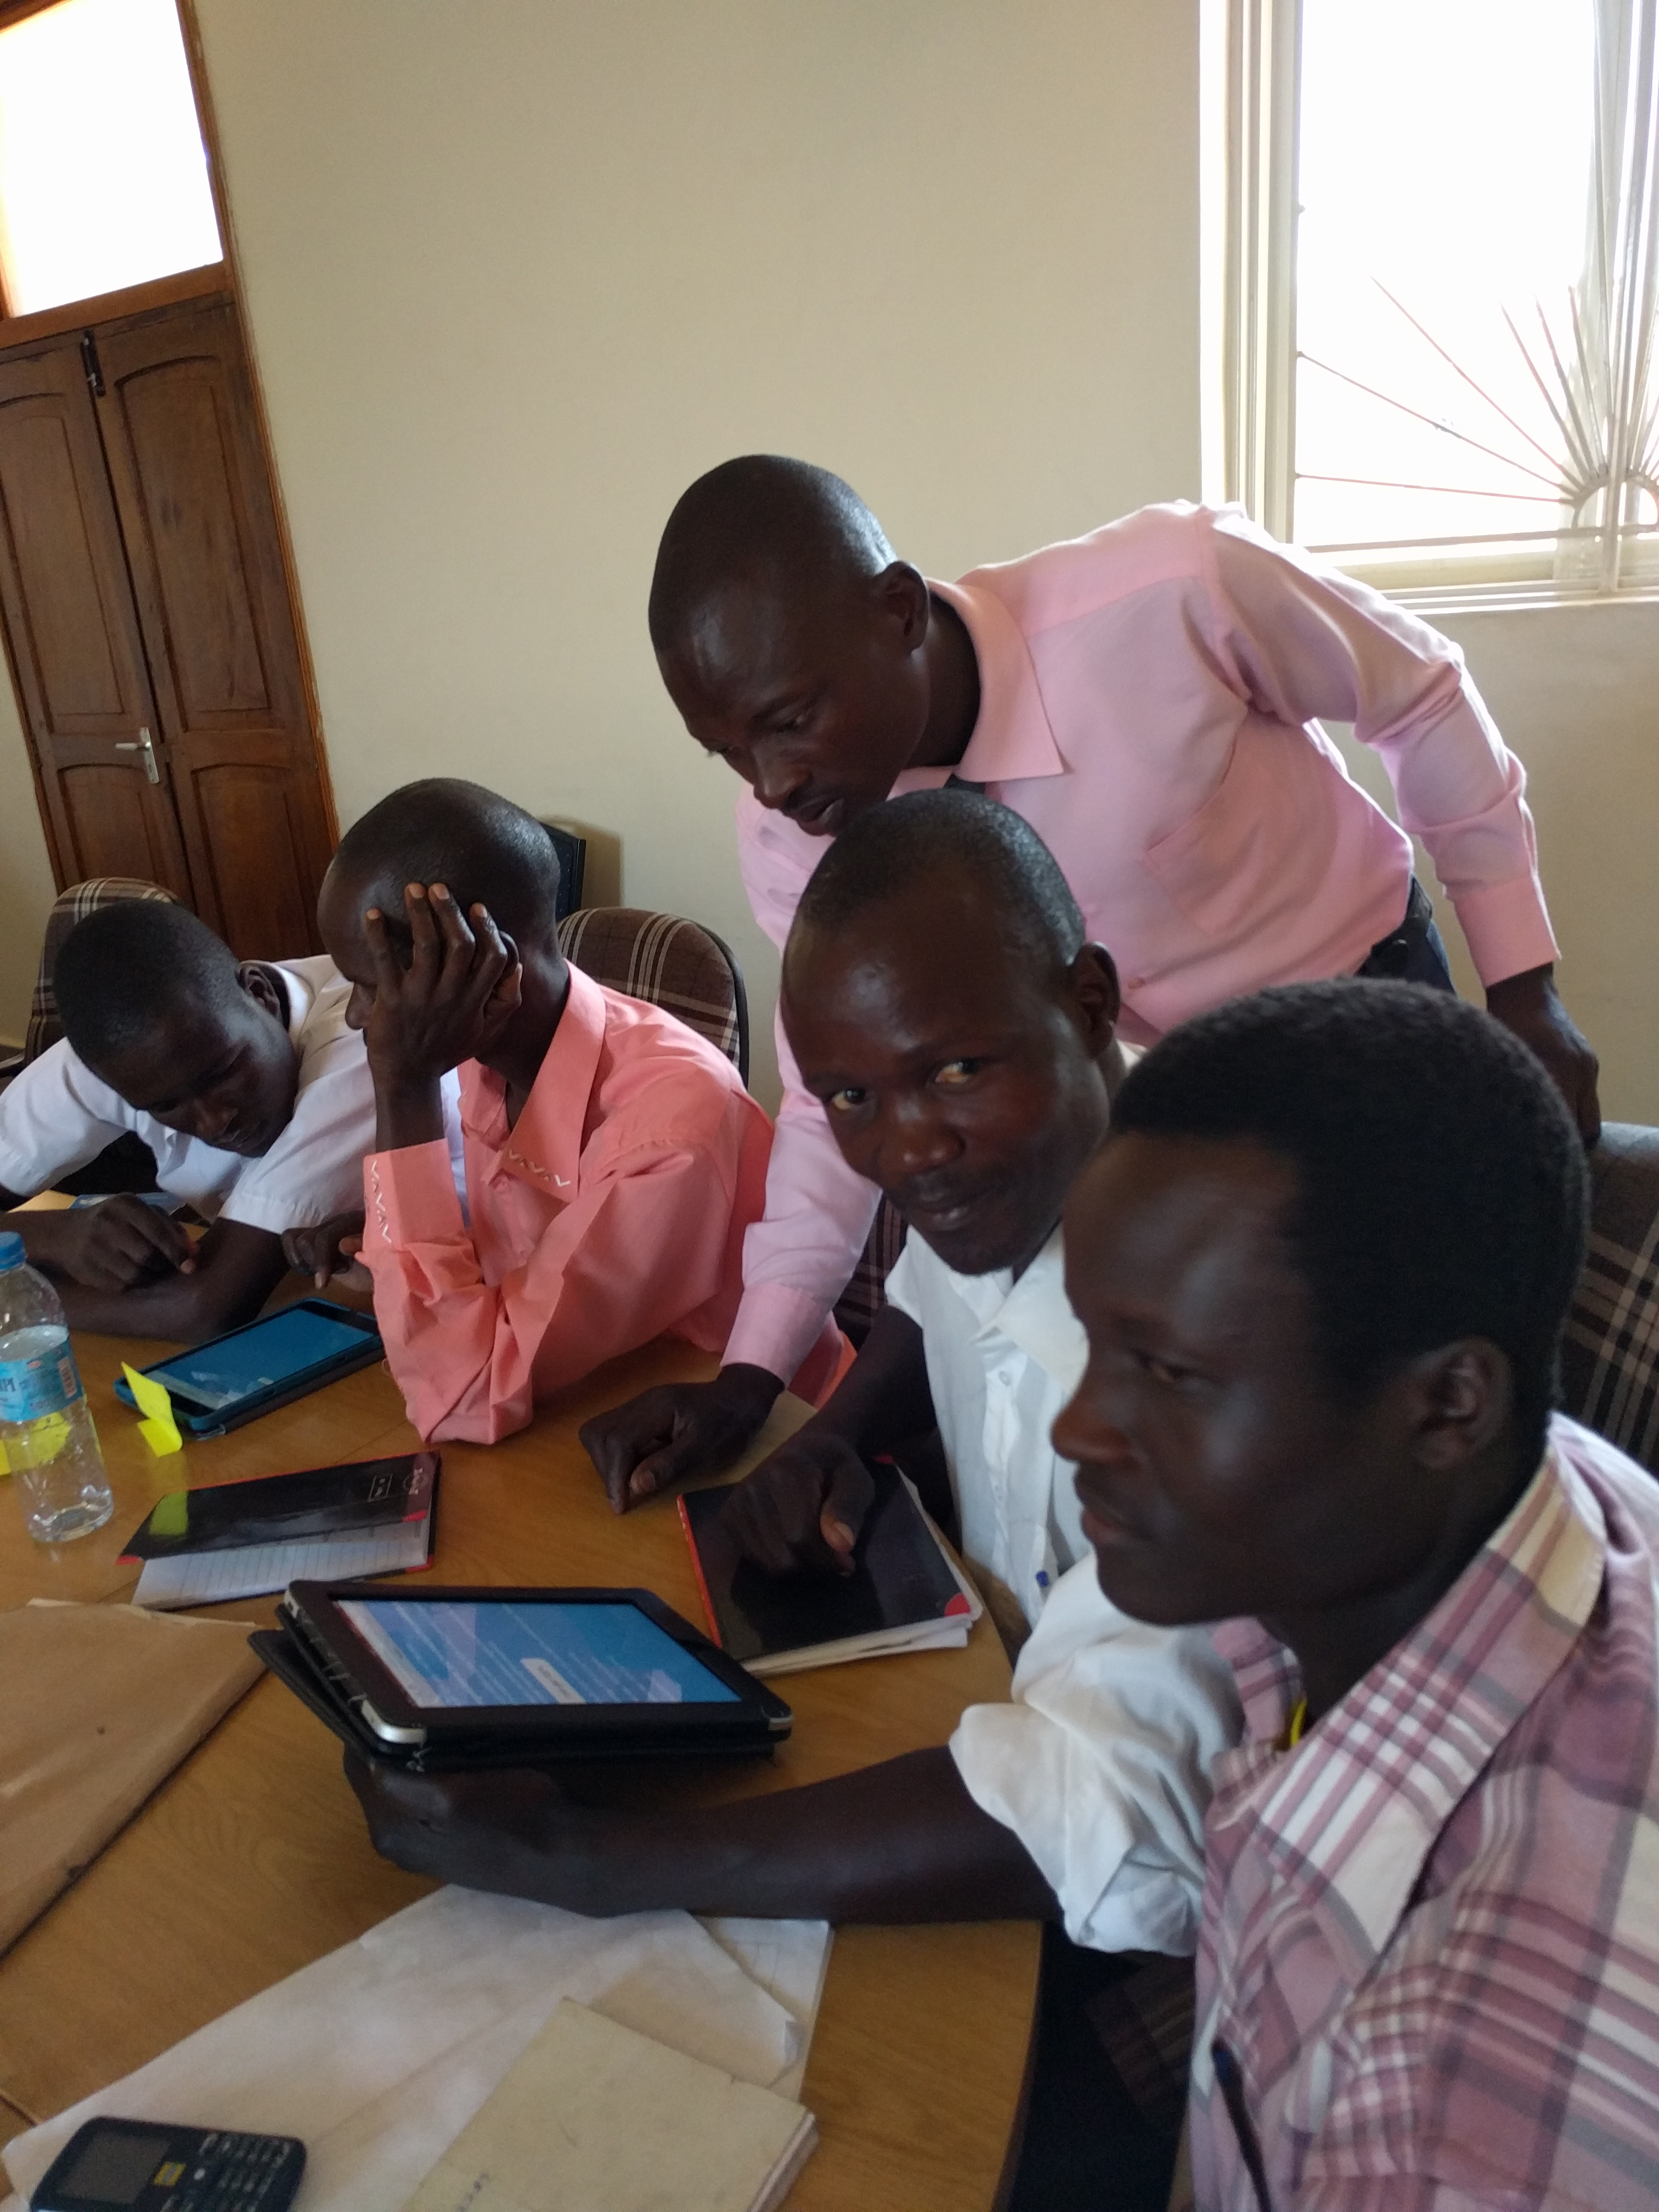
\includegraphics[width=0.4\textwidth]{iteration3/appTestTablet.jpg}
    \caption{Two coaches using a tablet for the formative app test. The coaches worked in pairs. After the app test, interviews was held, before co-creation workshops started.}
    \label{fig:tabletTest}
  \end{figure}

  \begin{figure}[h]
    \centering
    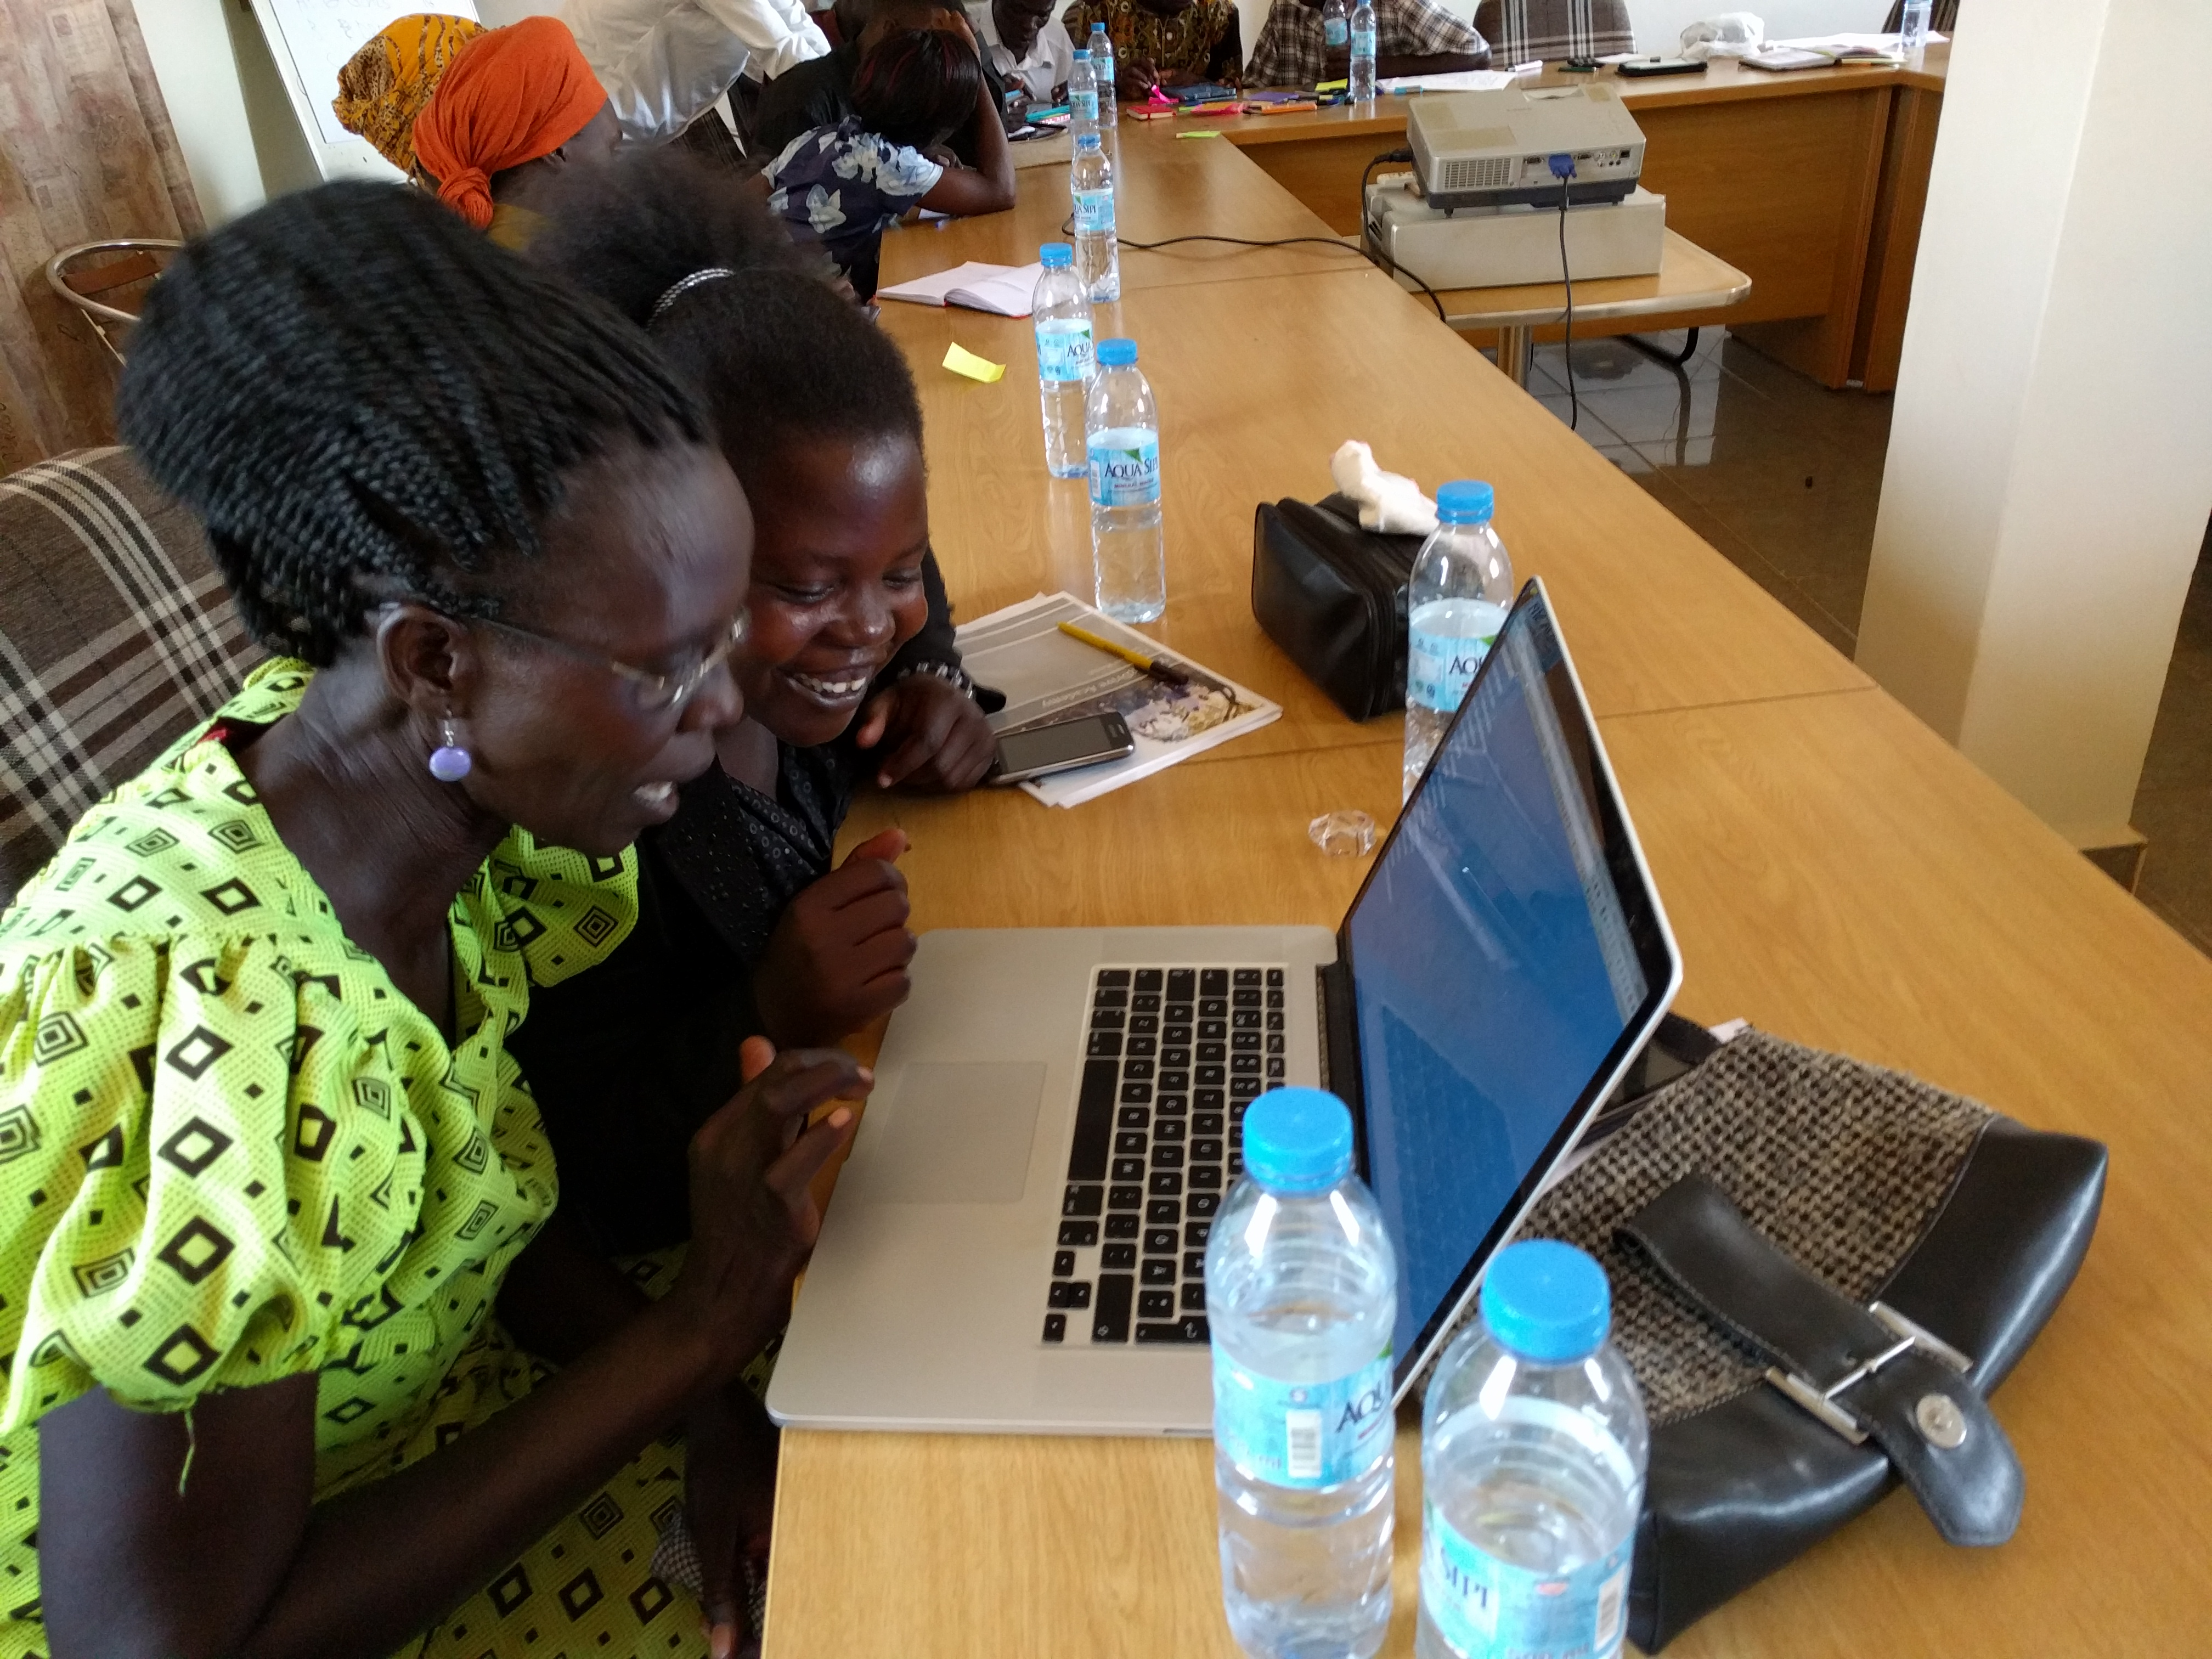
\includegraphics[width=0.8\textwidth]{iteration3/appTestComputer.jpg}
    \caption{A variation of smartphones and tablets were used. In one case, the battery died on one of the device so it needed to be replaced with a computer. It was the first time the coaches used a computer, and they learned quickly and eagerly.}
    \label{fig:computerTest}
  \end{figure}

  Regarding usability, the most negative thing from the app test, was that the app was not user friendly for first-time smartphone users. There were a lot of bugs, the most damaging for the app test being resizing of the font size for each new question, see figure \ref{fig:iteration-map} E-3. This forced some coaches to try to zoom on the devices, even if they did not know how. This could in turn cause refresh of the web page, and sometimes there was no Internet available. Thus, the data can not be fully reliable.

  This was the first time true frustration was shown. Out of 23 respondents, 7 rated the app easy, 11 medium, and 6 hard. This was not viable.

  Another reason for this, is that cognitive load seemed to be too high. The feedback was not scaffolded enough, so coaches did not have enough energy to assess all of their results carefully before taking the test again via "Improve". One user did not want to press "Improve" until having read the manual. The motivation was: "Not because that is what the info says, but because I can learn more from the manual, about more than what the questions says." This is in fact the preferred behaviour from Josefina, and the app should continue to further encourage only using the app training or certification mode after having prepared via the manual. This way, the app is still assessment, but it is "learning by thinking", with feedback. In iteration 4, comparing those that are allowed to use the manuals with those that are not allowed to, would be interesting.

  Regarding learning, four new ideas were tested during the app test, assessing the new pedagogical model of the app. Item 1-3 were tested in the app (the high-fidelity trigger material), and item 4 was tested via low-fidelity trigger material, asking a coach (and then the coach audience) if he or they could give the answers from memory without being shown alternatives.

  \begin{enumerate}
  \item "Try again"-button. When clicked, your wrong answers are repeated.
  \item If 100\% on the 1st try, gold. On 2nd try: silver. On 3rd try: bronze.
  \item Ask meta-cognitive questions, "Are you sure?", at the end of each question.
  \item Record your answer to the question before you are shown alternatives.
  \end{enumerate}

  Item 1, 2 and 3 were determined good after the interviews. Item 4 showed relevance, but implementation in the app would give many challenges (mainly how to assess if the coach could give the right answer without giving different alternatives. Voice recognition or free-form answers are hard to analyze, to implement, and to use by a first-time smartphone user).

  \clearpage

\subsection{Discussion}

  For iteration 3, the coaches could not only assess, but also \textit{learn} Correct Information, which was successful, but needs to be done more effectively. It took an unacceptable amount of time to reach 100\% proficiency on all the quizzes. This was especially evident, on the quiz on Correct Structure och Time Management, "Week 9: Are you ready?", when it took a coach 102 minutes to reach 100\% without errors. In iteration 2, when "Improve" did not exist, it probably would have taken even longer.

  For the first time both signs of learning via perceptual exposure (many questions during a limited time, by trial and error) and deliberate practice (via learning via reflection) could be identified from the app. It is just that the app as of now is quite inefficient, especially in terms of speed, so while the ideas are there, the criteria are not fulfilled.

  The focus had been on "I am well prepared", but also including "I am certified.". It was shown that most coaches does not care about the simple gamification aspect of "I am certified" (which the workshop already had shown) but that they do care about their learning progress and learning results. The app could further embrace this.

  If there is one thing additional learned during the iteration, it is the notion of "data is knowledge, and knowledge is power". A realization is that both the developer, the coaches, the teacher, and the project partners can gain important insights. Adding "Are you sure?" to each quiz question, coach understanding was amplified, because now, also the coach's attitude towards learning can be evaluated. See more about this in the Discussion chapter \ref{cha:discussion}.

  \subsection{Next iteration}
  To improve effectiveness for the next iteration, a couple of goals were chosen. While the app would work well for the Ugandian coach training, the use case of a youth session was not good enough yet. Mostly, this is in regards to that it takes too long time to improve via the app, and that the feedback is not sufficient.

  \begin{itemize}
    \item Improve Deliberate practice. The criteria for Deliberate practice is not fulfilled today.
    \begin{itemize}
      \item  Follow the recommendation to design so that knowledge in a topic can go from unreliable to 95\% reliability within one to three 45-90-minute sessions.
      \item If this is not possible from changing the learning tactic, don't continue trying: split the quizzes into smaller pieces \citep{sierra}.
    \end{itemize}
    \item Improve Perceptual expose
    \begin{itemize}
      \item Divide the learner's expertise according to \cite{sierra}, "Can't do", "Can do with effort", and "Can do effortlessly".
    \end{itemize}
    \item Increase the use of questions to prompt self-monitoring  and self-evaluation \citep{sitzmann}.
    \begin{itemize}
      \item Using "learning by thinking" and encouraging a growth mindset, can benefit reaching metacognitive skills on Bloom's revised taxonomy.
      \item Help the coach to analyze and evaluate its own learning, possibly improving faster in the app.
    \end{itemize}
    \item Improve feedback to reflect that the teacher does not want to encourage coaches to have their youth session before they are 100\% confident with the material
    \item Data collection needs to be online and needs to be individual
    \begin{itemize}
      \item To do it online means that there needs to be a database, but also a login, so individuals are traceable.
    \end{itemize}
  \end{itemize}


\section{Iteration 4: Uganda Summative Test}

Here the results from the qualitative and quantitative data for iteration 4 are shown, together with conclusions.

\subsection{Analysis of Interviews}

The answers given during the three group interviews has been summarized and clustered into three areas, see figure \ref{fig:overview}. Further, the answers within interaction design has been clustered into its four main principles, see figure \ref{fig:interactiondesign}. The questions regarding learning has tried to answer why a coach is correct or incorrect on a given question, see figure \ref{fig:learning}. Service design has been clustered into the two questions "When do you want to use the app?" and "When are you not able to use the app?", see figure \ref{fig:servicedesign}. Zoomed-in versions of all of the areas are presented after the overviews, where the analysis of the quotes can be seen in its fullest. The quotes from these mind-maps are individual, which means that if another coach has had a similar thought, their quote is branched next to the following quote.

\begin{figure}[h]
    \centering
    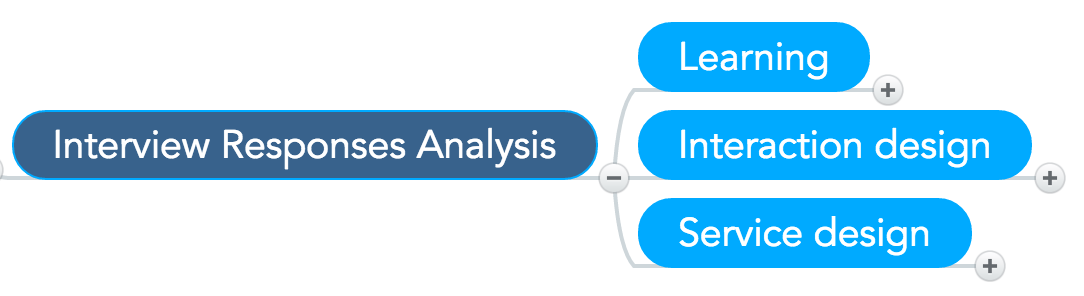
\includegraphics[width=0.3\textwidth]{analysis/interviews/overview_notexpanded.png}
    \caption{The interview answers has been clustered into three areas: learning, interaction design and service design.}
    \label{fig:overview}
\end{figure}

\begin{figure}[h]
    \centering
    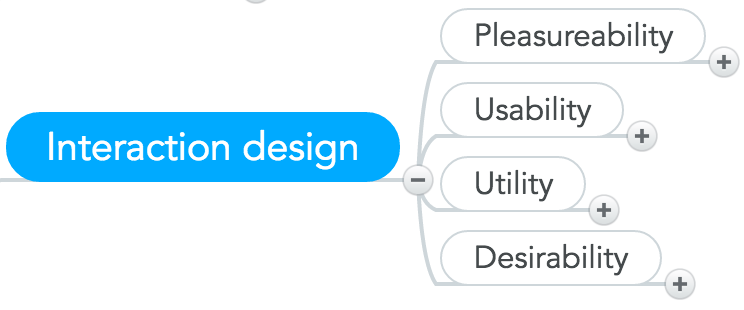
\includegraphics[width=0.3\textwidth]{analysis/interviews/interactiondesign_notexpanded.png}
    \caption{The coach quotes regarding interaction design has been divided by four criteria: pleasurability, usability, utility and desirability.}
    \label{fig:interactiondesign}
\end{figure}

%For learning and service design, the analysis of the interview quotes can bee seen in its fullest in figure \ref{fig:learning} and figure \ref{fig:servicedesign} respectively. Zoomed-in versions of all of the areas are presented after the overviews, where the analysis of the quotes can be seen in its fullest.

\begin{figure}[h]
    \centering
    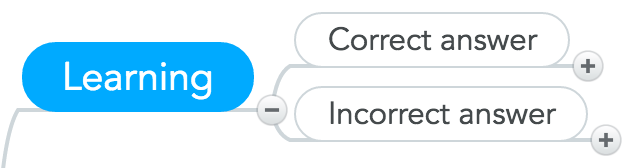
\includegraphics[width=0.3\textwidth]{analysis/interviews/learning_notexpanded.png}
    \caption{The coach quotes regarding learning has been divided by if they give insight to why a coach has been correct or incorrect on a given question.}
    \label{fig:learning}
\end{figure}

\begin{figure}[h]
    \centering
    
\includegraphics[width=0.3\textwidth]{analysis/interviews/servicedesign_notexpanded.png}
    \caption{The coach quotes regarding service design has been divided into \textit{when} you want to use the YoungDrive app, and when you are hindered from doing so.}
    \label{fig:servicedesign}
\end{figure}

\clearpage

\subsubsection{Learning}\label{sec:interview-learning}

By reading the quotes from the coaches carefully, it can be understood why answers can appear correct by the coaches (see figure \ref{fig:learning1}), even if this would not be the case (see figure \ref{fig:learning2}.

\begin{figure}[h]
    \centering
    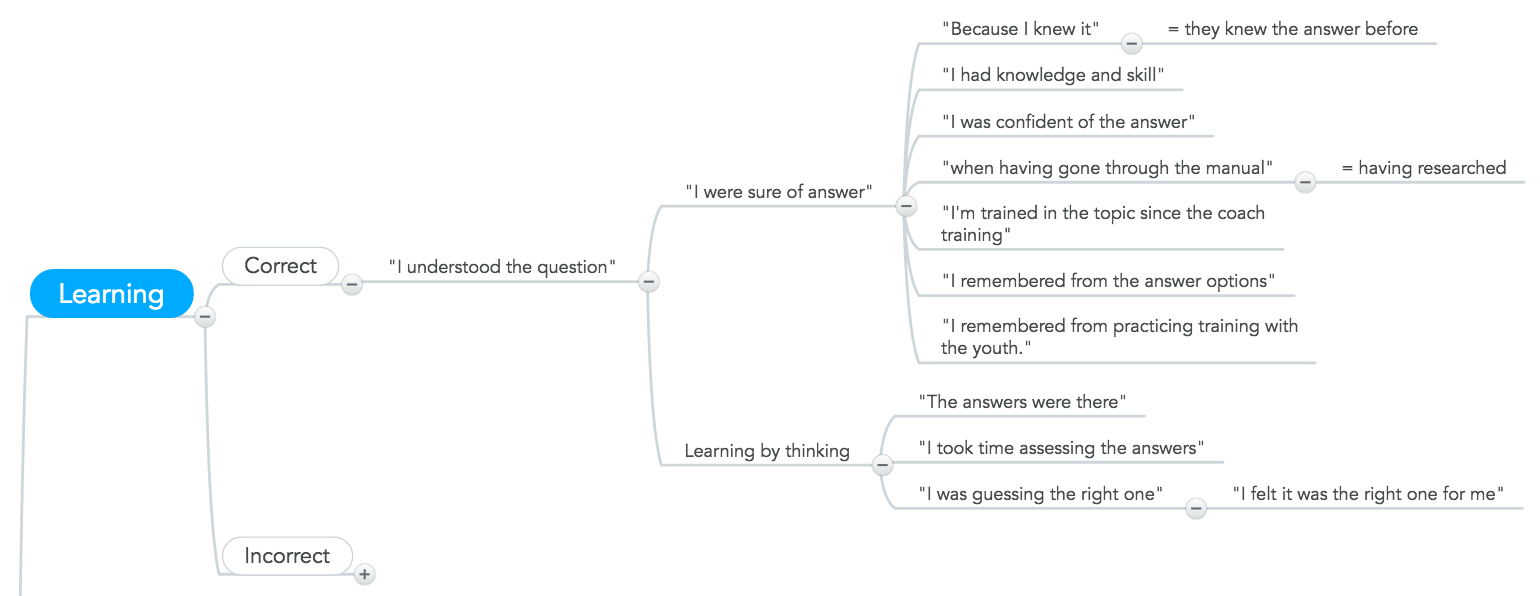
\includegraphics[width=1.0\textwidth]{analysis/interviews/learning_correct.png}
    \caption{Quotes explaining why a coach could give an correct answer on a given question. Either you were sure of the answers, or you made a qualified guess. A prerequisite for answering the question correct is that you understood the questions meaning.}
    \label{fig:learning1}
\end{figure}

\begin{figure}[h]
    \centering
    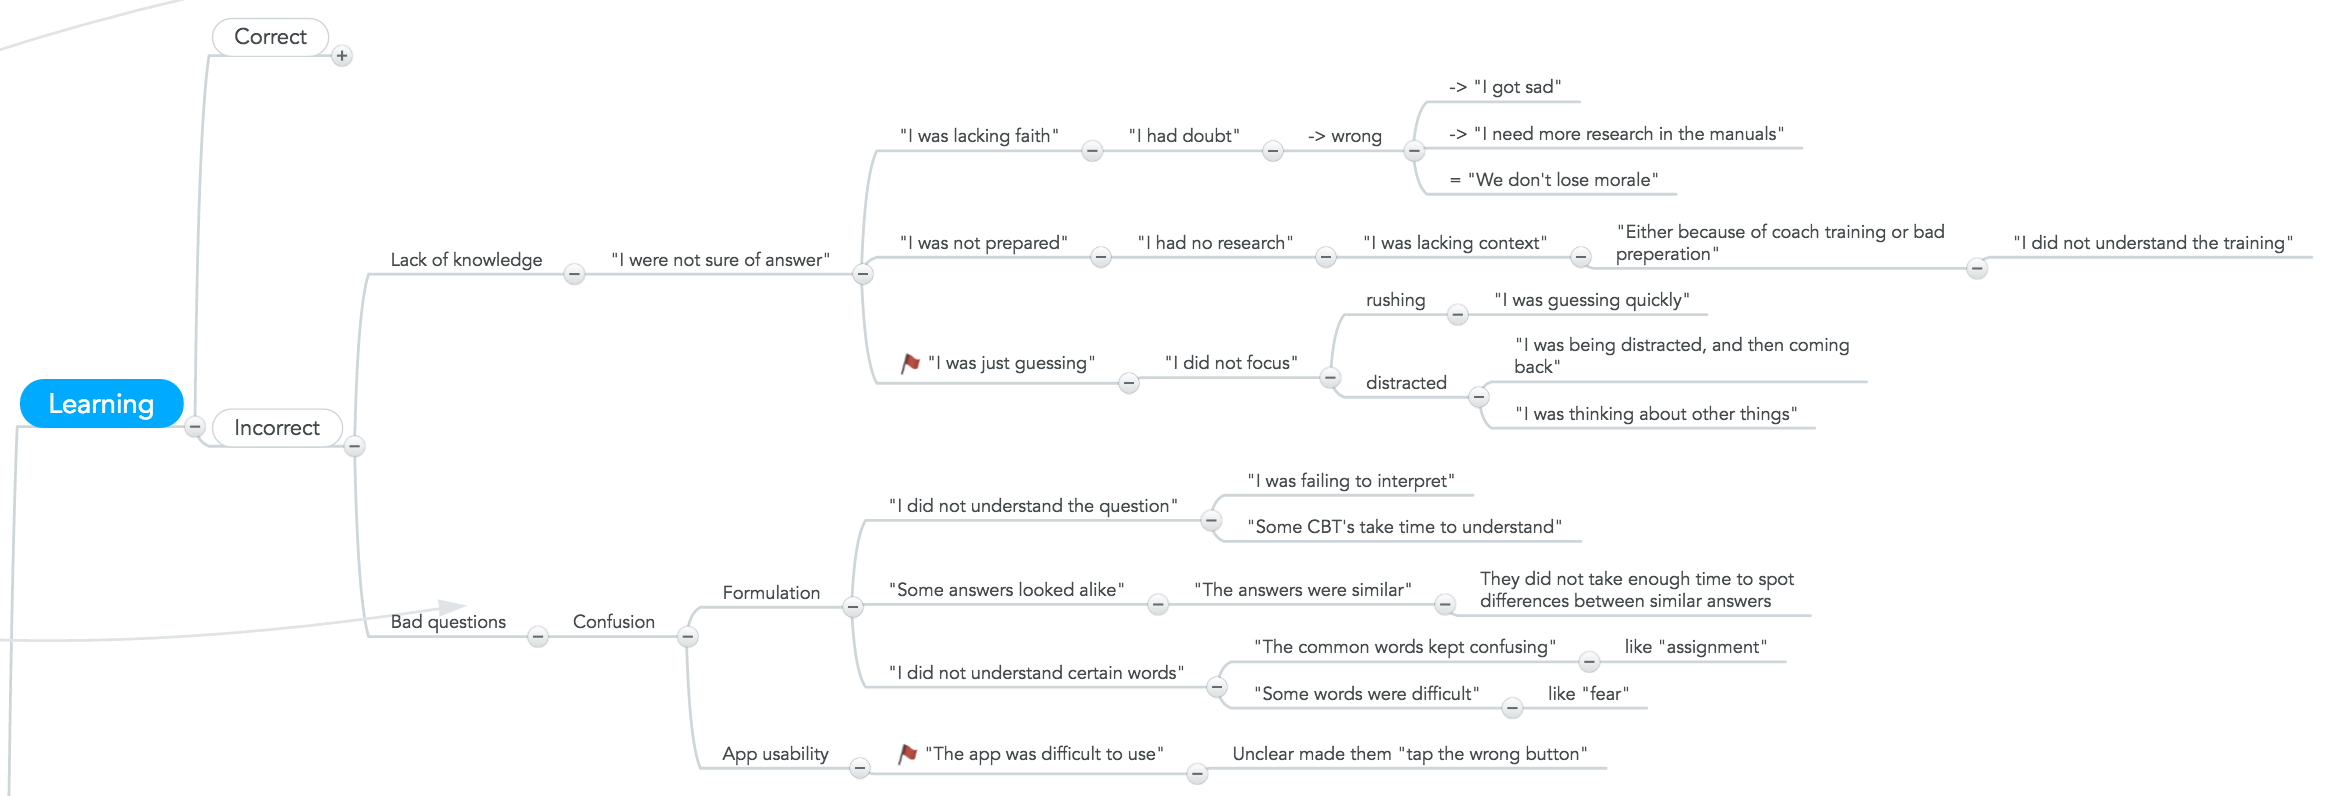
\includegraphics[width=1.0\textwidth]{analysis/interviews/learning_incorrect.png}
    \caption{Quotes explaining why a coach could give an incorrect answer on a given question. Either, the coach did not have sufficient knowledge to answer the question confidently (for a number of reasons, given in the figure), or the question was not understood correctly, or the app usability was a hindrance.}
    \label{fig:learning2}
\end{figure}

\clearpage

\subsubsection{Interaction Design}

Most importantly, in the final app test, everyone thought the app was good and easy to use (n = 26). This is important, as this had not been the case in iteration 3. Regarding the four different areas of interaction design, positive remarks on utility are especially beneficial for learning. However, pleasurability, usability and desirability is a prerequisite for the app to be used by the coaches. For desirability, if the coaches are stimulated by using the app, two reviews were: "It felt good using the app" and "It motivated learning". The other three interaction principles (pleasurability, usability and utility) have been given their own mind-map below, see figure \ref{fig:interaction1}, figure \ref{fig:interaction2} and \ref{fig:interaction3}.

\begin{figure}[h]
    \centering
    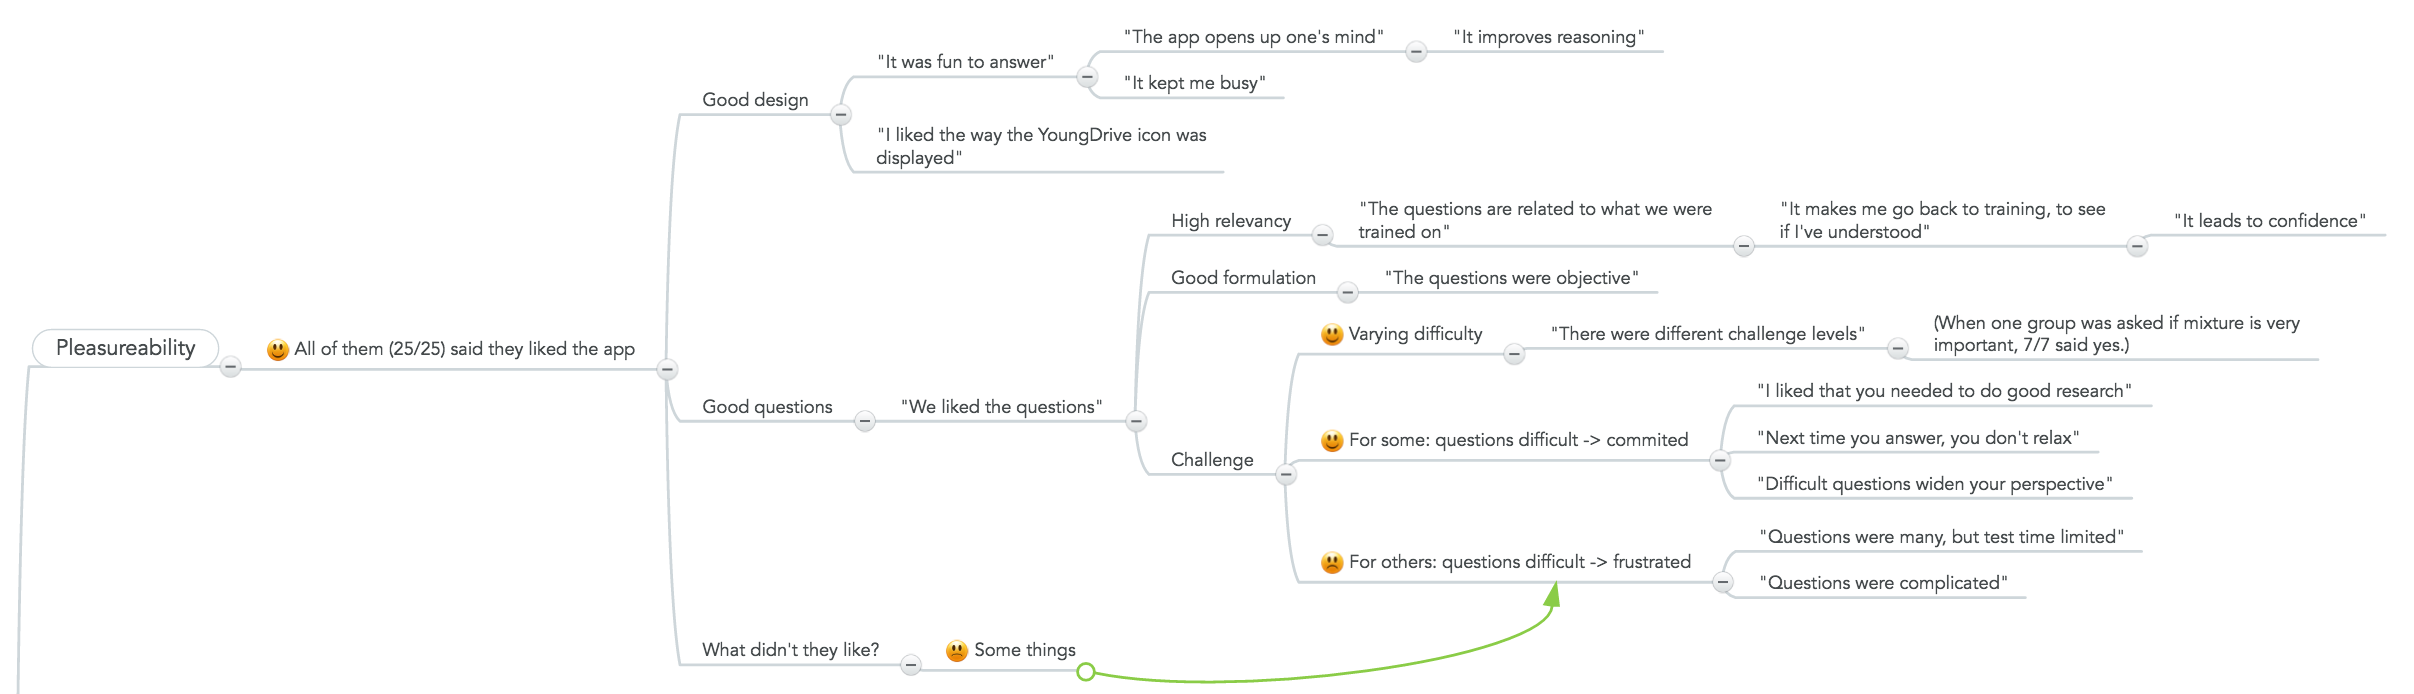
\includegraphics[width=1.0\textwidth]{analysis/interviews/interactiondesign_pleasurability.png}
    \caption{Pleasurability was 100\%, as the app had a good design and well-motivated questions, however some coaches were frustrated by difficult questions in the app, or the time needed to complete a quiz during the workshop.}
    %From the interviews, it is visible that the coaches feel the quizzes has been a fair way to measure their knowledge in the topic. The answer "It leads to confidence" could show that when a coach has done a quiz reaching certification, they do feel more confident about teaching the topic.
    %Positively, assessment of "Am I ready?" can happen already before the youth session, in the app.}
    \label{fig:interaction1}
\end{figure}

\begin{figure}[h]
    \centering
    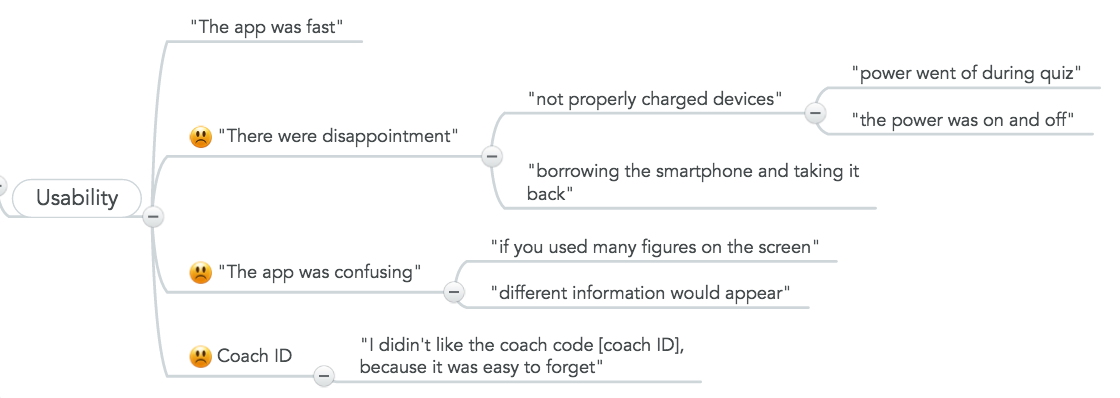
\includegraphics[width=1.0\textwidth]{analysis/interviews/interactiondesign_usability.png}
    \caption{Usability. As previosuly stated, all of the coaches (25/25) thought the app was easy to use when asked by raise of hands. However, in the interviews, some detailed comments regarding usability appeared. Regarding workshop issues, some of the devices' battery died during the workshop, or needed to be replaced. Regarding the app, some still mention too much information to appear at once, or that information are shown that the coach does not expect. Only one coach mentioned thinking that thee login was not user friendly, since the Coach ID was easy to forget. The Coach ID has since been documented by the local project leaders, so they can be contacted in such situations.}
    \label{fig:interaction2}
\end{figure}

\begin{figure}[h]
    \centering
    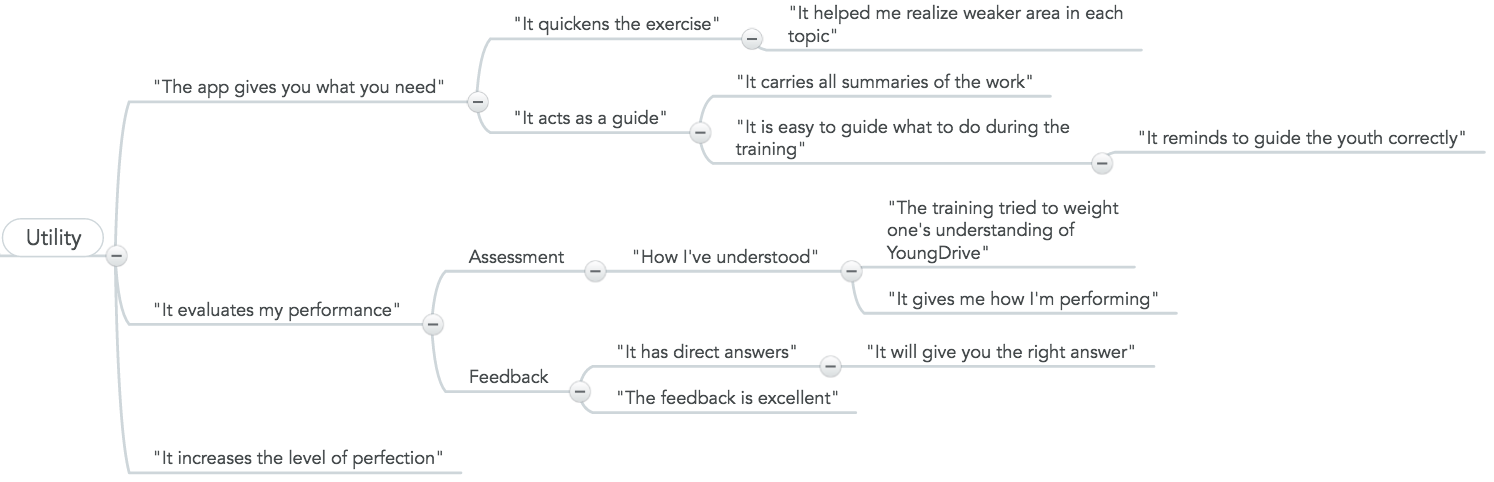
\includegraphics[width=1.0\textwidth]{analysis/interviews/interactiondesign_utility.png}
    \caption{Utility gives a valuable measure of what benefits the coach finds with using the app. Quotes regarding usefulness are: "It quickens the exercise", "It carries all summaries of the work", "It reminds to guide the youth correctly". For training, coaches conclude that "It evaluates my performance" and that "The feedback is excellent". One coach summarizes with "It increases the level of perfection".}
    \label{fig:interaction3}
\end{figure}

\clearpage

\subsubsection{Service Design}

It is important to understand if and when the app will be used by the coach, and if the environment of the coach in any way can hinder use of the app. For understanding the coach situation to these two criteria, see figure \ref{fig:servicedesign1} and \ref{fig:servicedesign1}.

\begin{figure}[h]
    \centering
    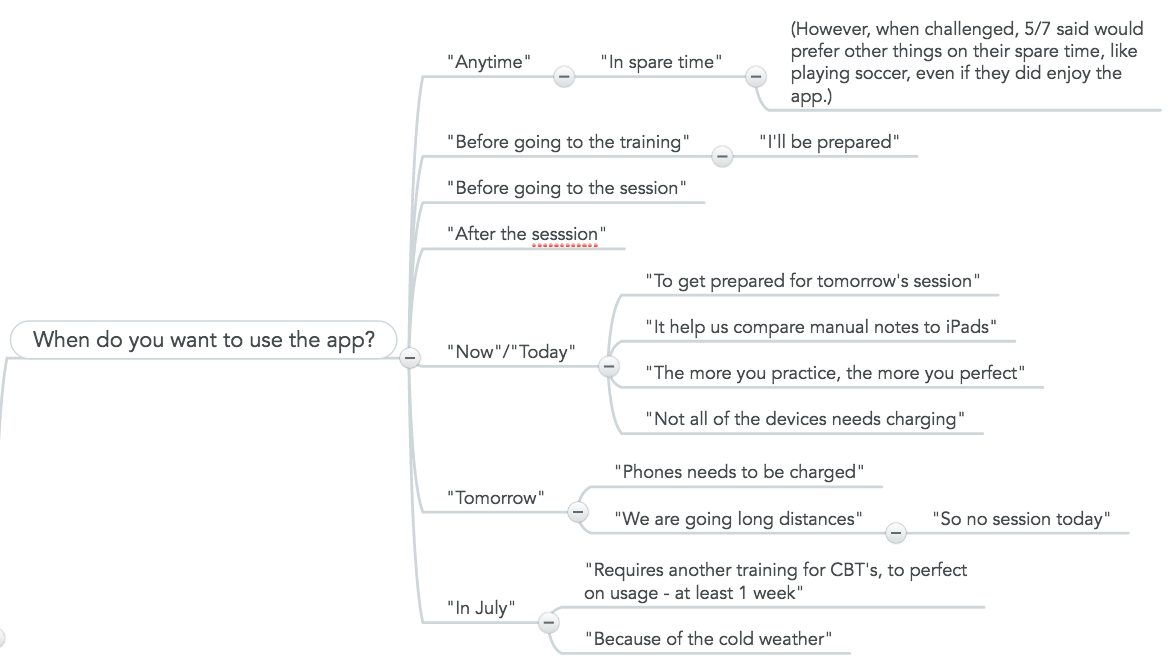
\includegraphics[width=1.0\textwidth]{analysis/interviews/servicedesign_when.png}
    \caption{There are very varying answers to the question "When do you want to use the app?". Most coaches would have liked to use the app immediately. Some of the coaches identified the need for devices, more training, or charging of devices in being able to do so.}
    \label{fig:servicedesign1}
\end{figure}

\begin{figure}[h]
    \centering
    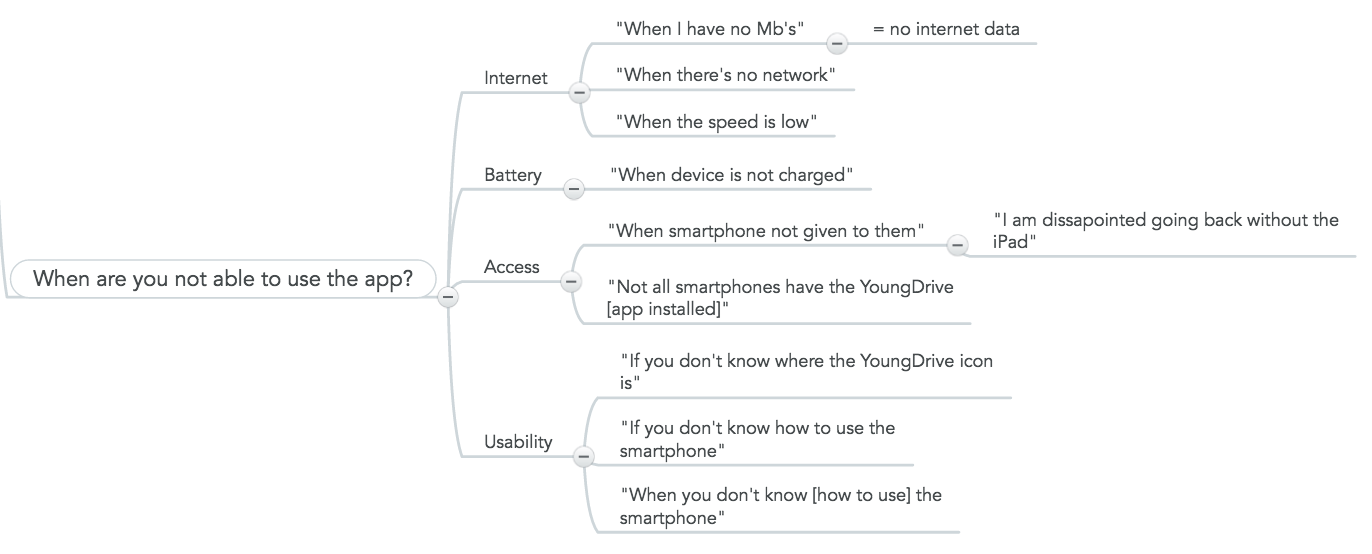
\includegraphics[width=1.0\textwidth]{analysis/interviews/servicedesign_cant.png}
    \caption{Answers for the question "When are you not able to use the app?" are grouped into four segments: internet issues, battery issues, low or no access to smartphones, or if the app is not usable because it is not available on the smartphone, or the coach does not know how to use a smartphone.}
    \label{fig:servicedesign2}
\end{figure}

\clearpage

\subsection{Analysis of Quiz Results}

    %What the data said

    % Christine och Patrick berättade senare att i regel presterar Young Mentor lite bättre än CBT, enligt deras rakningar. (från iteratoin 1 - stämde detta?)

    % Relevans av att testa financial literacy: "Precis som med förra gruppen, verkar ekonomin vara det svåraste att förstå (dolda utgifter, hur gå med vinst), som youth." (från iteration 1)

% Important to be objective
% En diskussion om hur resultaten kan användas i praktiken är också i de flesta fall belysande och relevant i rapporter

% https://liu.se/ias/kontakta-oss?l=en

For the first time, automatic data collection was used, which increased the amount of quantitative data that could be analysed substantially. Below, the findings from each data analysis method are presented. There was one test group and one reference group, the difference being if they were allowed to consult the manuals or only use the feedback from the app.

\subsubsection{Quiz Results and Pre-Test Data Analysed in Google Sheets}
For results gathered and analysed within the Google Sheet, see figure \ref{fig:analysFarg3}. For a zoomed in version, see Appendix \ref{cha:appendix4}. Early observations from the pre-test data when inserted into Google Sheets was that a surprising number of cells were left blank. One user had not done the pre-test (see column for coach 220), where some had left questions unanswered (most commonly "Do you own a company?" (should have used the word "business"), plus "Hours of preperation" and "Occations for a youth session" (there is a tendency this might be because they were not proud of their answers, because of correlations with low quiz results).

\begin{figure}[h]
    \centering
    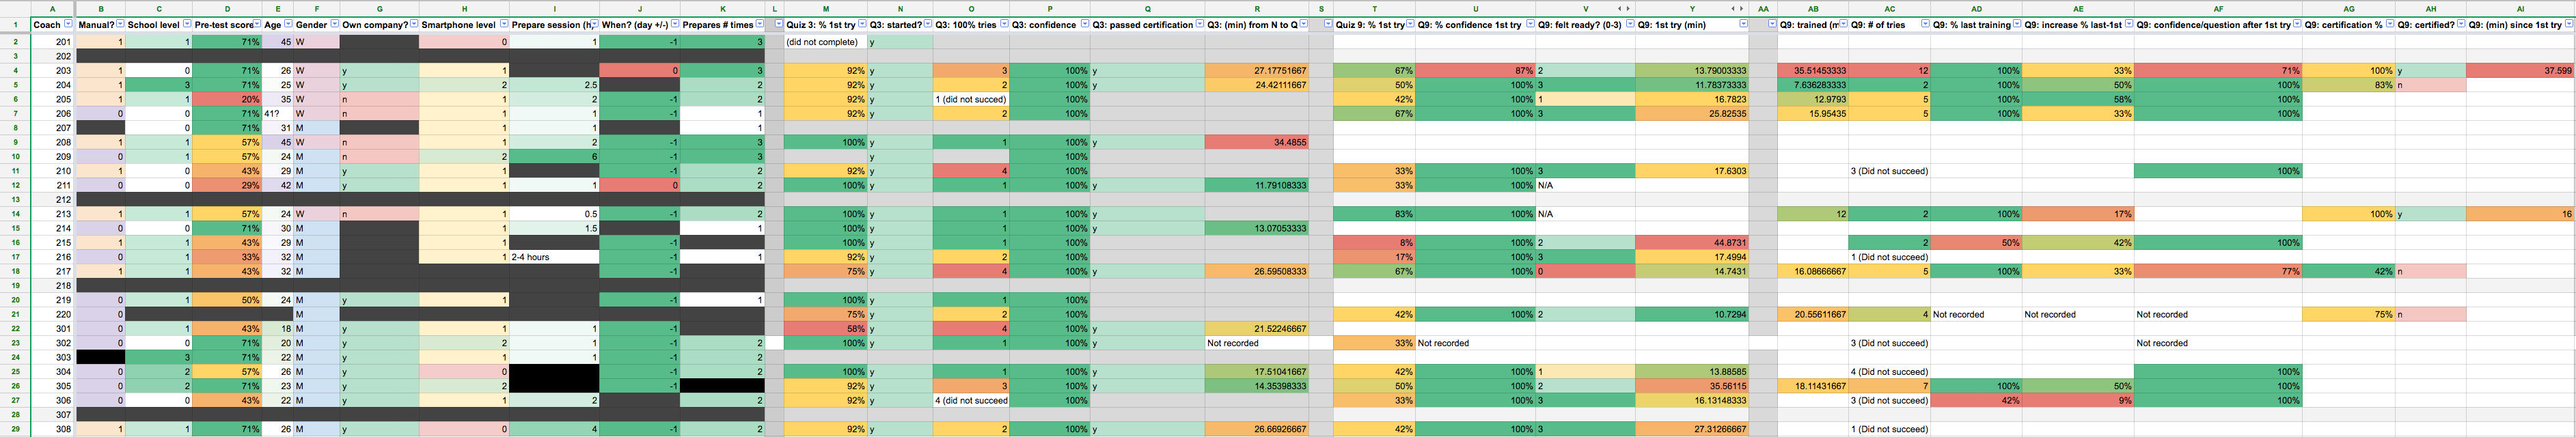
\includegraphics[width=1.0\textwidth]{analysis/sheets/0Overview.png}
    \caption{The Google Sheet after merging the pre-test data and the summed quiz results data. See zoomed-in versions and explanations for each section below.}
    \label{fig:analysFarg3}
\end{figure}

\begin{figure}[h]
    \centering
    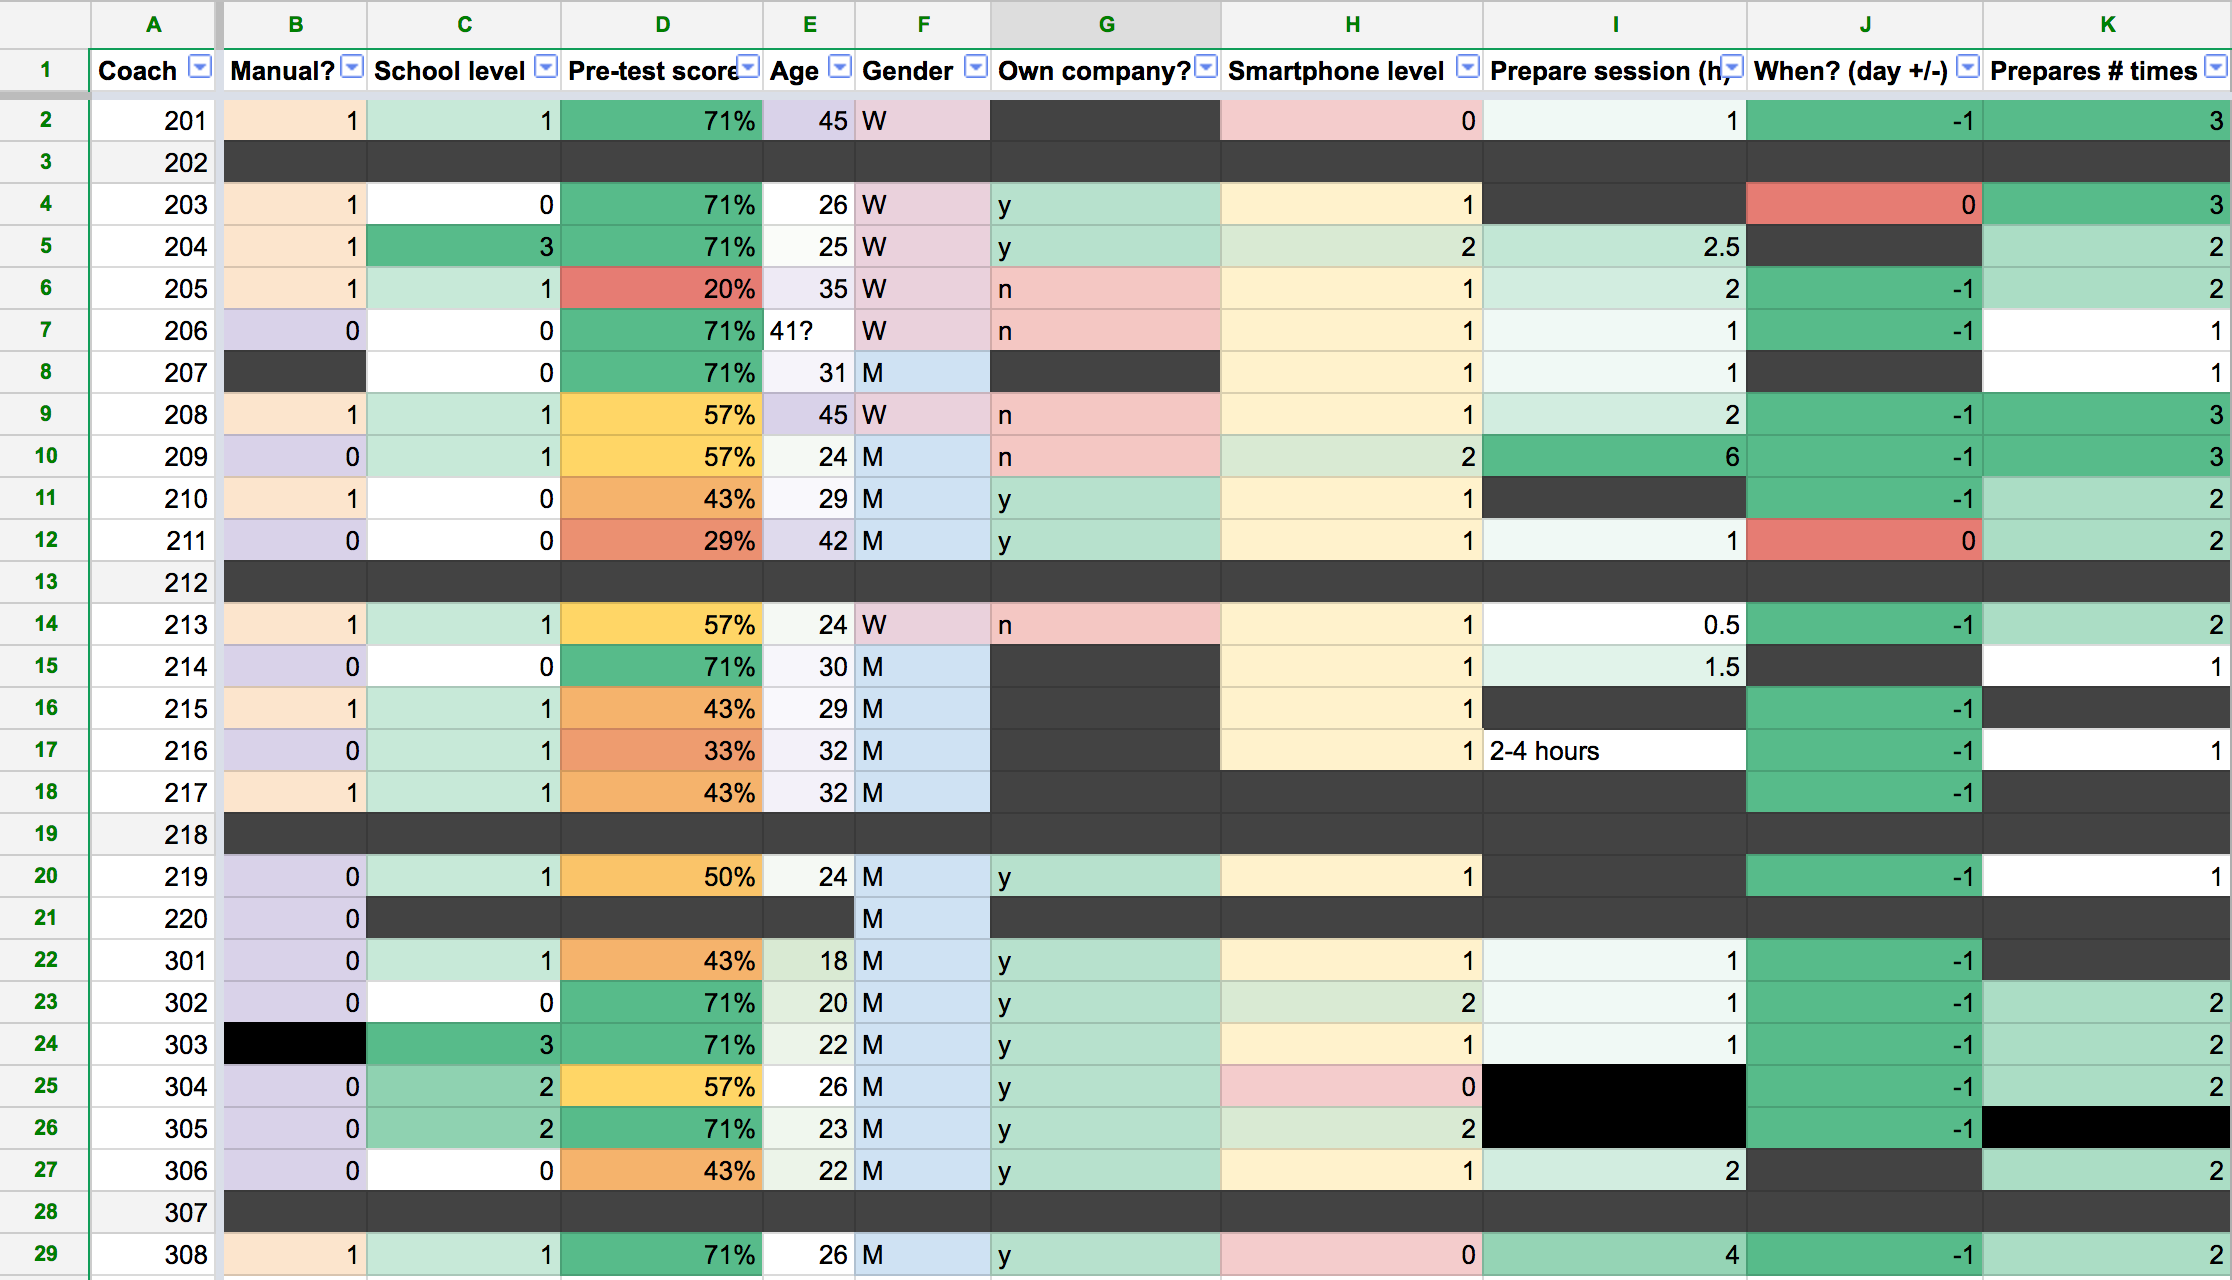
\includegraphics[width=1.0\textwidth]{analysis/sheets/1Pre-data.png}
    \caption{Pre-test data}
    \label{fig:1Pre-data}
\end{figure}

\begin{figure}[h]
    \centering
    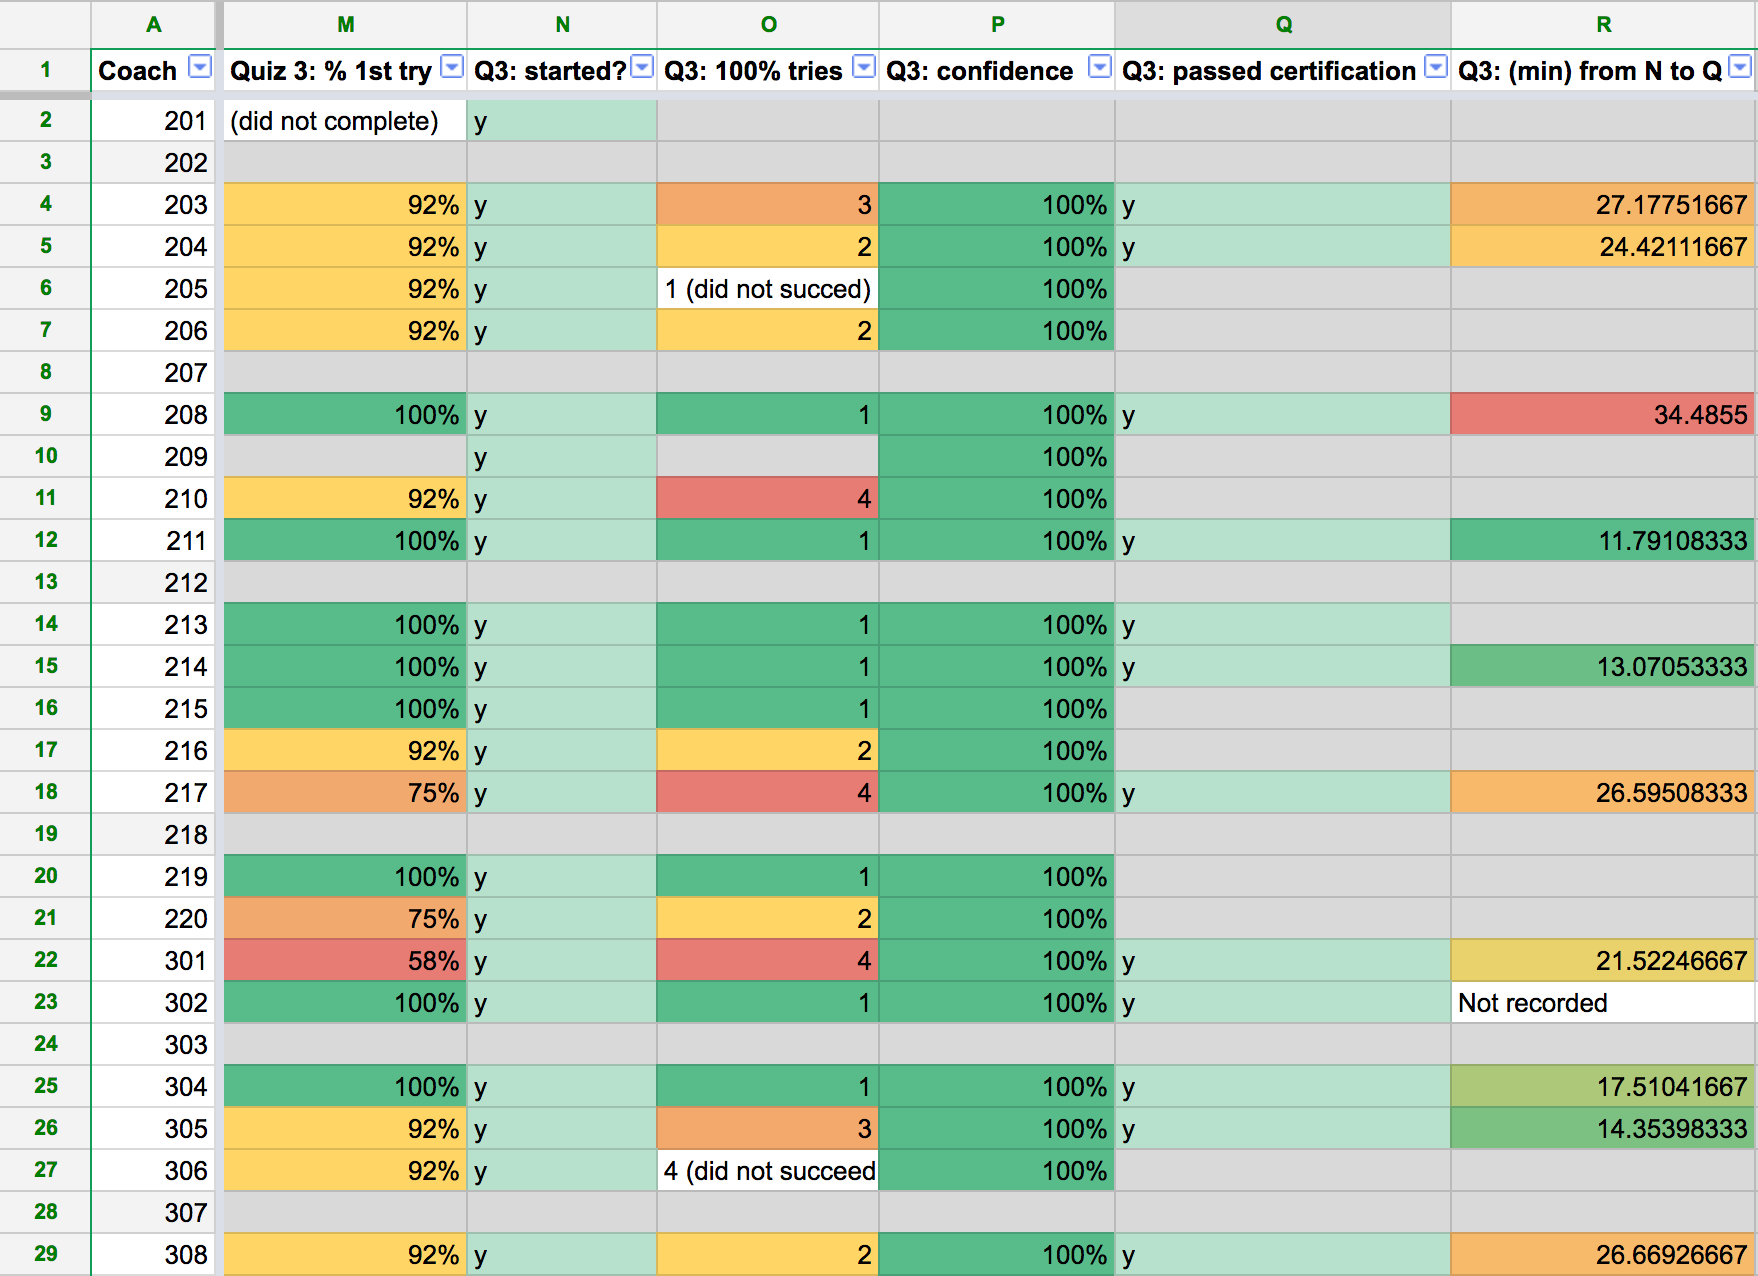
\includegraphics[width=1.0\textwidth]{analysis/sheets/2Quiz3.png}
    \caption{Quiz 3 answers.}
    \label{fig:2Quiz3}
\end{figure}

\begin{figure}[h]
    \centering
    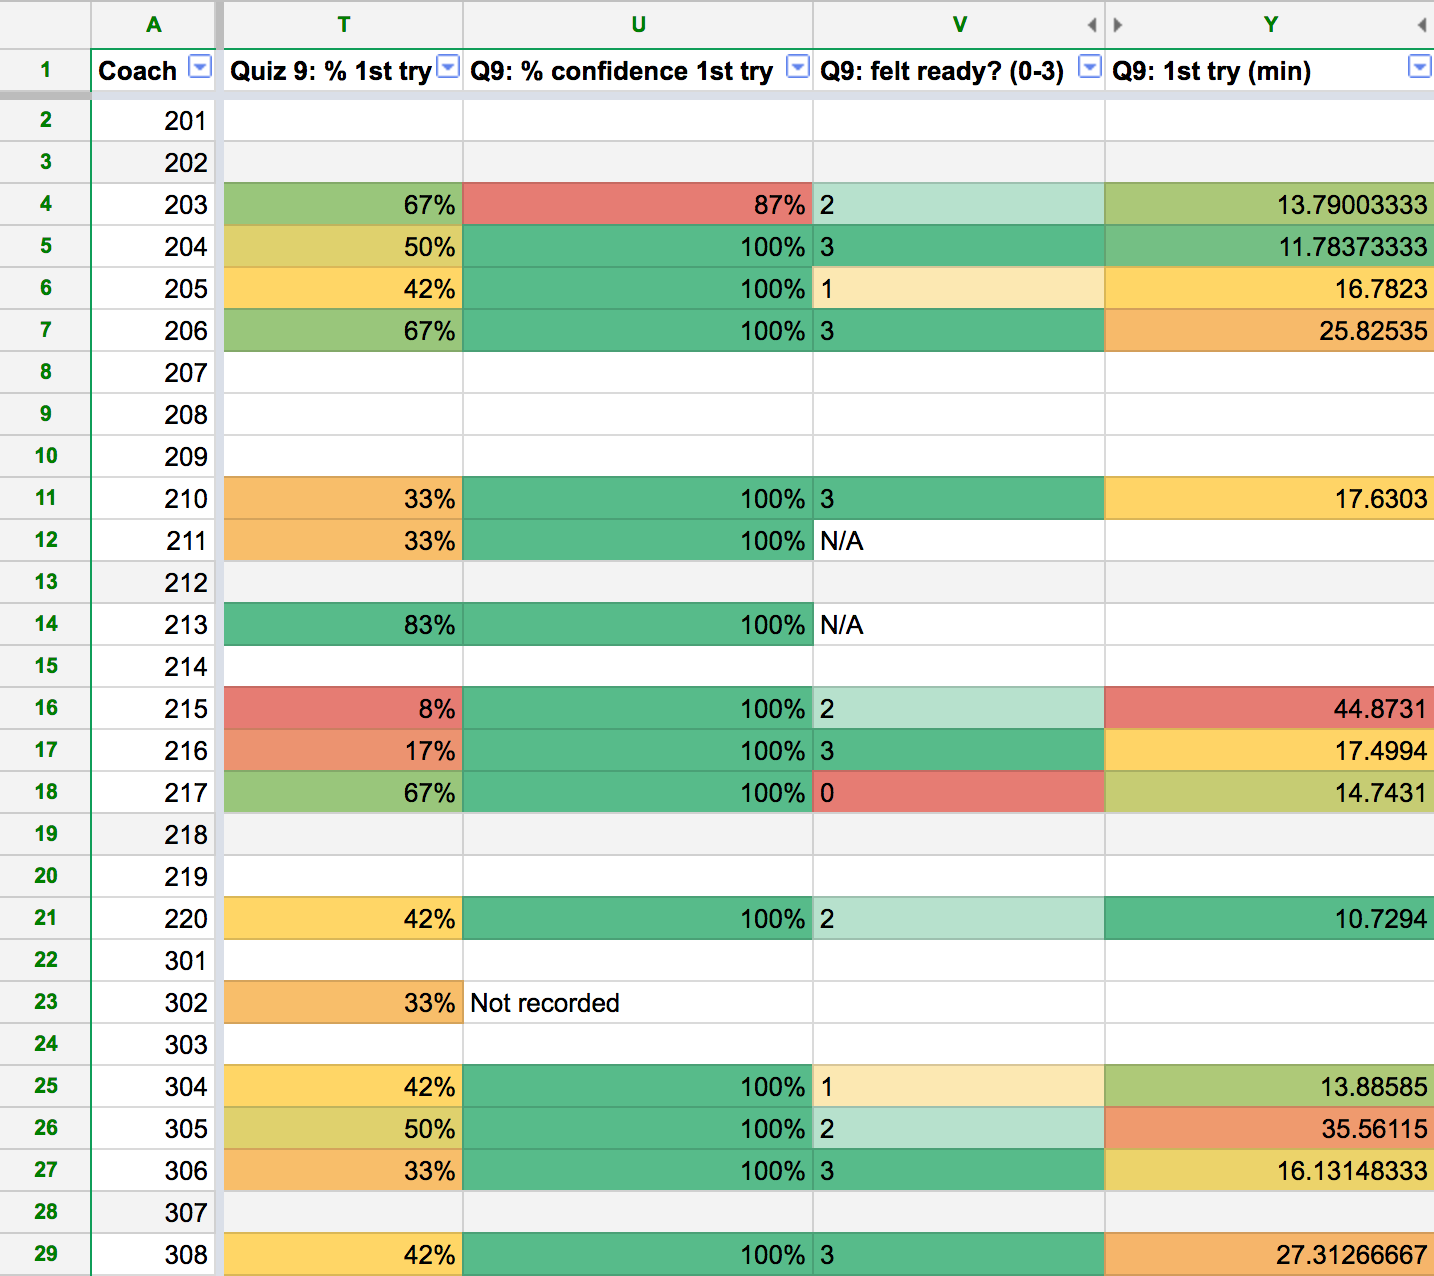
\includegraphics[width=1.0\textwidth]{analysis/sheets/3Quiz9A.png}
    \caption{Quiz 9 try 1 answers (correctness and recorded confidence ("Are you sure?": "Yes/No") on coach guide quiz 9 "Are you ready?", together with answering "How comfortable and ready do you feel right now to carry out session 9? (There is no right answer, just be honest with yourself!", alternative 1-4 ("Not ready at all", "Somehow ready", "Ready" or "Very ready and comfortable"). Finally in column Y, the time it took for the coach to complete quiz try 1 is given.}
    \label{fig:3Quiz9A}
\end{figure}

\begin{figure}[h]
    \centering
    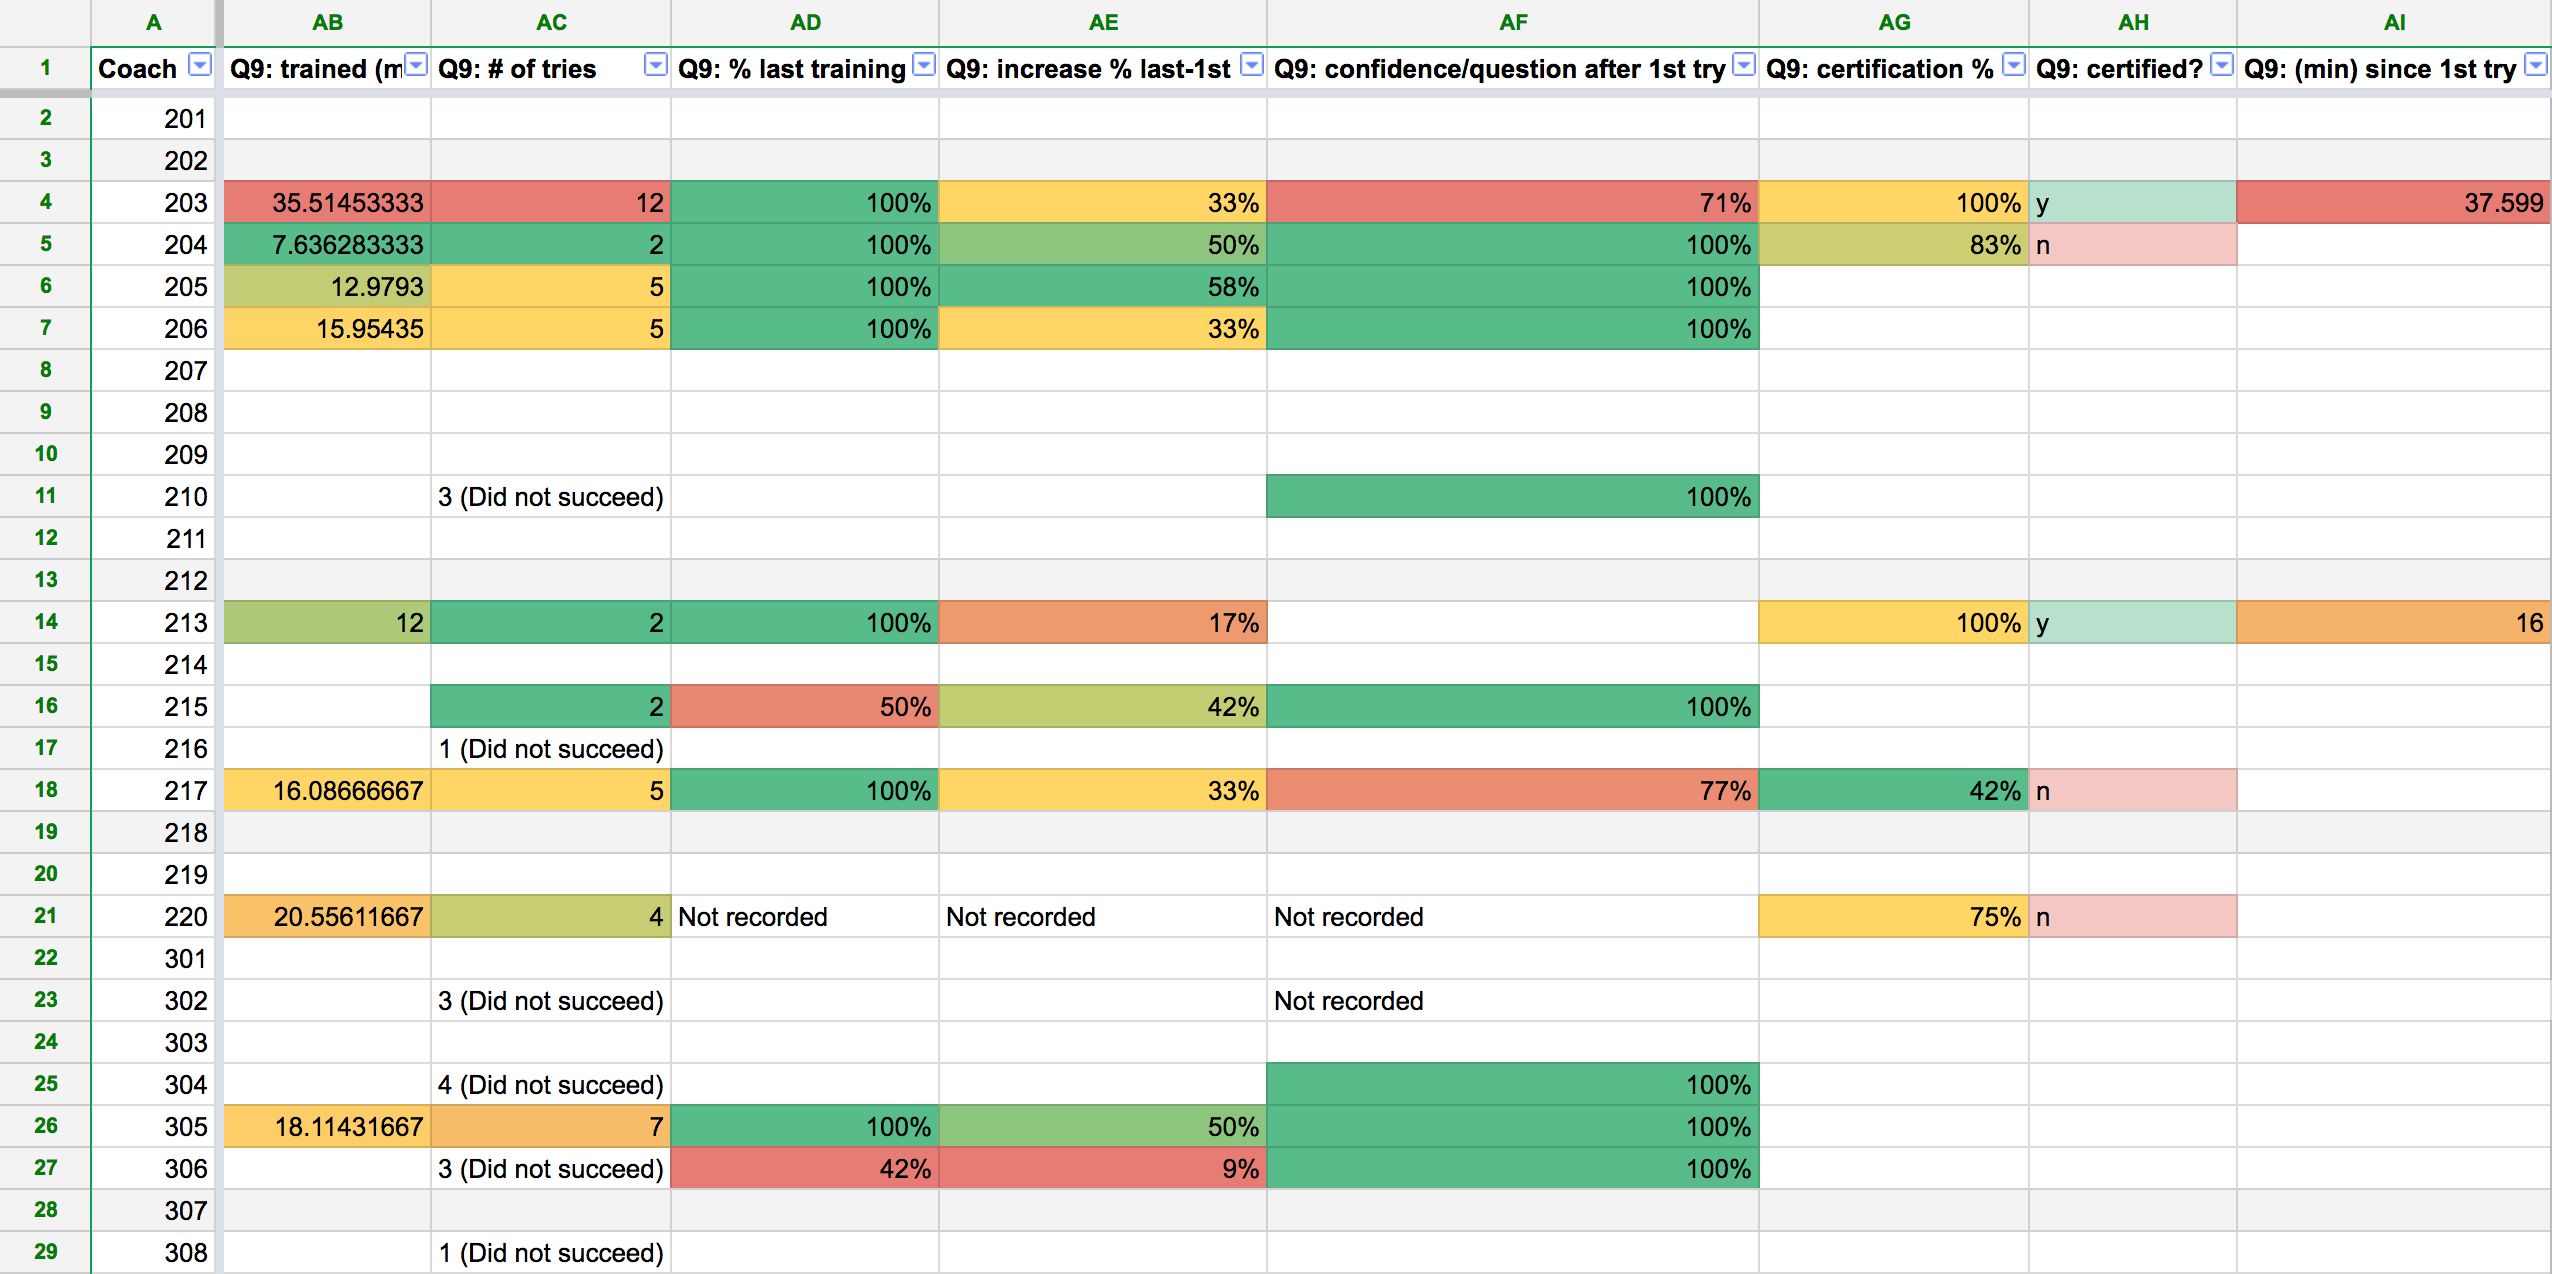
\includegraphics[width=1.0\textwidth]{analysis/sheets/3Quiz9B.png}
    \caption{Quiz results on the training and certification of coach guide quiz 9 "Are you ready?". Column AB: how many minutes they spent in training. AC: how many times they pressed "Try again", retaking the wrong answers. AD: their score on the last training quiz they took. AE: the increase from their first training to their last. AF: recorded "Are you sure?": "Yes/No" after taking the quiz try 1. Finally, for the coaches that started the certification, their results are shown, together with the time the quiz took for those that got 100\% correct on the first try.}
    \label{fig:3Quiz9B}
\end{figure}

\begin{figure}[h]
    \centering
    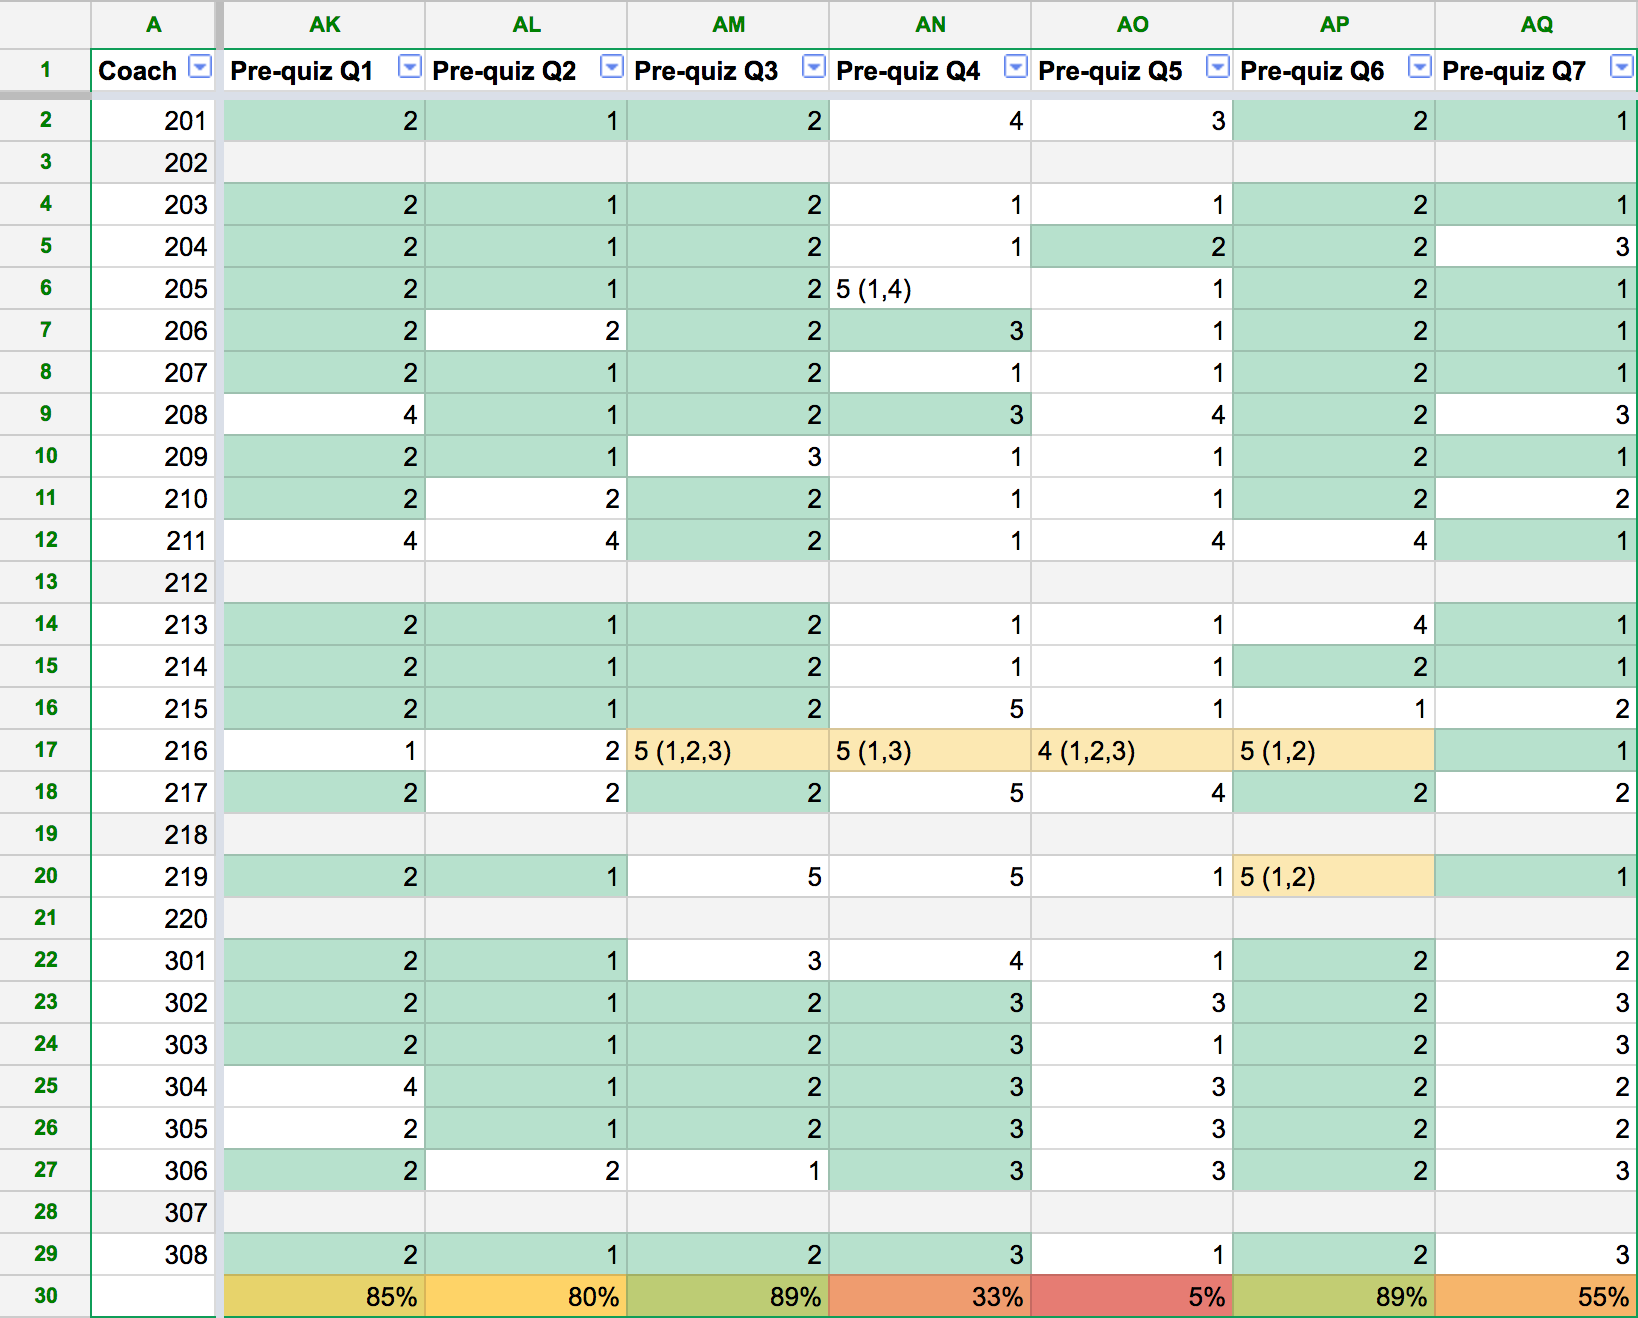
\includegraphics[width=1.0\textwidth]{analysis/sheets/4Pretest.png}
    \caption{Pre-quiz results per question and coach. The correct answers are given in green. The questions asked can be observed in Appendix \ref{cha:pre-test}}.
    \label{fig:4Pretest}
\end{figure}

\clearpage

Missing cells was not as obvious with the app results, were users could not progress in a quiz without answering both the question and the confidence. However, none of the passed quiz 9 certification answers had been submitted. Thus, it was needed to add these from the manual recordings, which had been used as a backup in case anything like this would happen.

There were a number of quick insights that could be drawn before the parallel coordinates visualization, simply by looking at the data as a spreadsheet.

It was believed that smartphone users feeling like novices might have a disadvantage with the app, since they will not learn as fast as experienced users. The interactions shows however, between iteration 3 to 4, almost all of the coaches does not feel intermediate instead of beginners using the smartphone and the YoungDrive app. The quiz data verifies this, with no direct correlation between technical skills and quiz results (comparing column H "Smartphone level" 1-3) with column M and T (quiz scores on the first try for quiz 3 and 9). From the pre-test data, it can be seen that only CBTs said they didn't feel comfortable with smartphone (n=2, column H, of which there were 6 Youth Mentors and 14 CBTs). A reason might be age, as CBTs were older than the Youth Mentors. Also, youth mentors had higher school level than the CBTs. More probable, is that the experience of using a smartphone since iteration 3 has matured over time, and that they are now more confident. %It is interesting that this has improved since iteration 3, possibly indicating that the smartphone skills have matured since the last test two weeks ago.

From the Google Sheets quiz results data, it could be seen that there was a surprisingly low number of answers where the user answered the question without confidence (see column P, U and AF). This is not good for feedback purposes, as answers were actually often not correct.

First-hand insights before the parallel coordinates were that there was a strong correlation between pre-quiz results (column D) and quiz 9 try 1 (column T), and slightly visible also in quiz 3 try 1 (column M), but with more outliers. Also, with manuals there was a higher probability of finishing quiz 9 training and certification (see also findings from the parallel coordinates visualization below). The data shows small tendencies that being honest and deliberate during the training increases the likelihood that a coach can get 100\% without faults, and has truly learned.

The final version of the app shows users can get 100\% on quiz results much faster (column R, AB and AI) than the previous version, as the score board had been improved for iteration 4. Since the target group in Zambia and Uganda was different, it is hard to empirically prove if it went faster getting 100\% with the possibility of repeating only the wrong questions, asking "Are you sure?", and providing individual feedback. Asking after the app does in iteration 4 does show however, that 100\% of the coaches now thought the feedback was good for learning.

%\subsubsection{Bonus Result: Learnings from Observing All of the Quiz Results}
Also, from observing all of the quiz submissions (see sample in figure \ref{fig:unprocessedData}), more users had started a quiz without finishing it than anticipated. This speaks for usability issues (cancelling the quiz by mistake, like clicking the back button, or loss of internet access) or bad technical skills (needs to design to be more fail-safe) or lack of motivation (needs to design for unmotivated coaches as well. The need group of "challenged coaches" might need other design than "ideal coaches".

Finally, a lot of users had done quizzes that were not Topic quiz 3 and Coach quiz 9, which might indicate high interest (if they did more than 2 quizzes) or confusion (if they did not do 3 or 9, but they did do other quizzes) during the app evaluation. This meant that on some aspects, there were less data than anticipated, (which was troublesome, as there were already few data points), and some aspects where there was more data than anticipated (on overlooked other quizzes).

\subsubsection{Parallel Coordinates Visualization}
Statistical analysis in R showed that none of the results were statistically significant to be notable using linear regression, or any of the other statistical methods detailed in the methodical framework. It was believed that statistical analysis could at least give insight into what to look for in the parallel coordinates visualization, but also for this, a larger sample would be needed. An interactive parallel coordinates visualization could give many more insights, more faster than the static presentations in Google Sheets or statistical analysis in R.

There is an almost infinite number of findings and observations that are interesting to look at via the parallel coordinates visualization. Even if there are no clear correlations (which are often found immediately when working with large data sets and parallel coordinates), tendencies can be found. As nothing is statistically significant (mostly because of the small data sample), the only thing that could be found are tendencies, and to analyze outliers. Then, these findings was critically analyzed to characteristics, and observations made from the app tests. As such, the data should be seen as indications of where future research is interested, and not as universal truths. For further research into the data, see figure \ref{fig:parallellCoordinates3} and the below sections.

\begin{figure}[h]
    \centering
    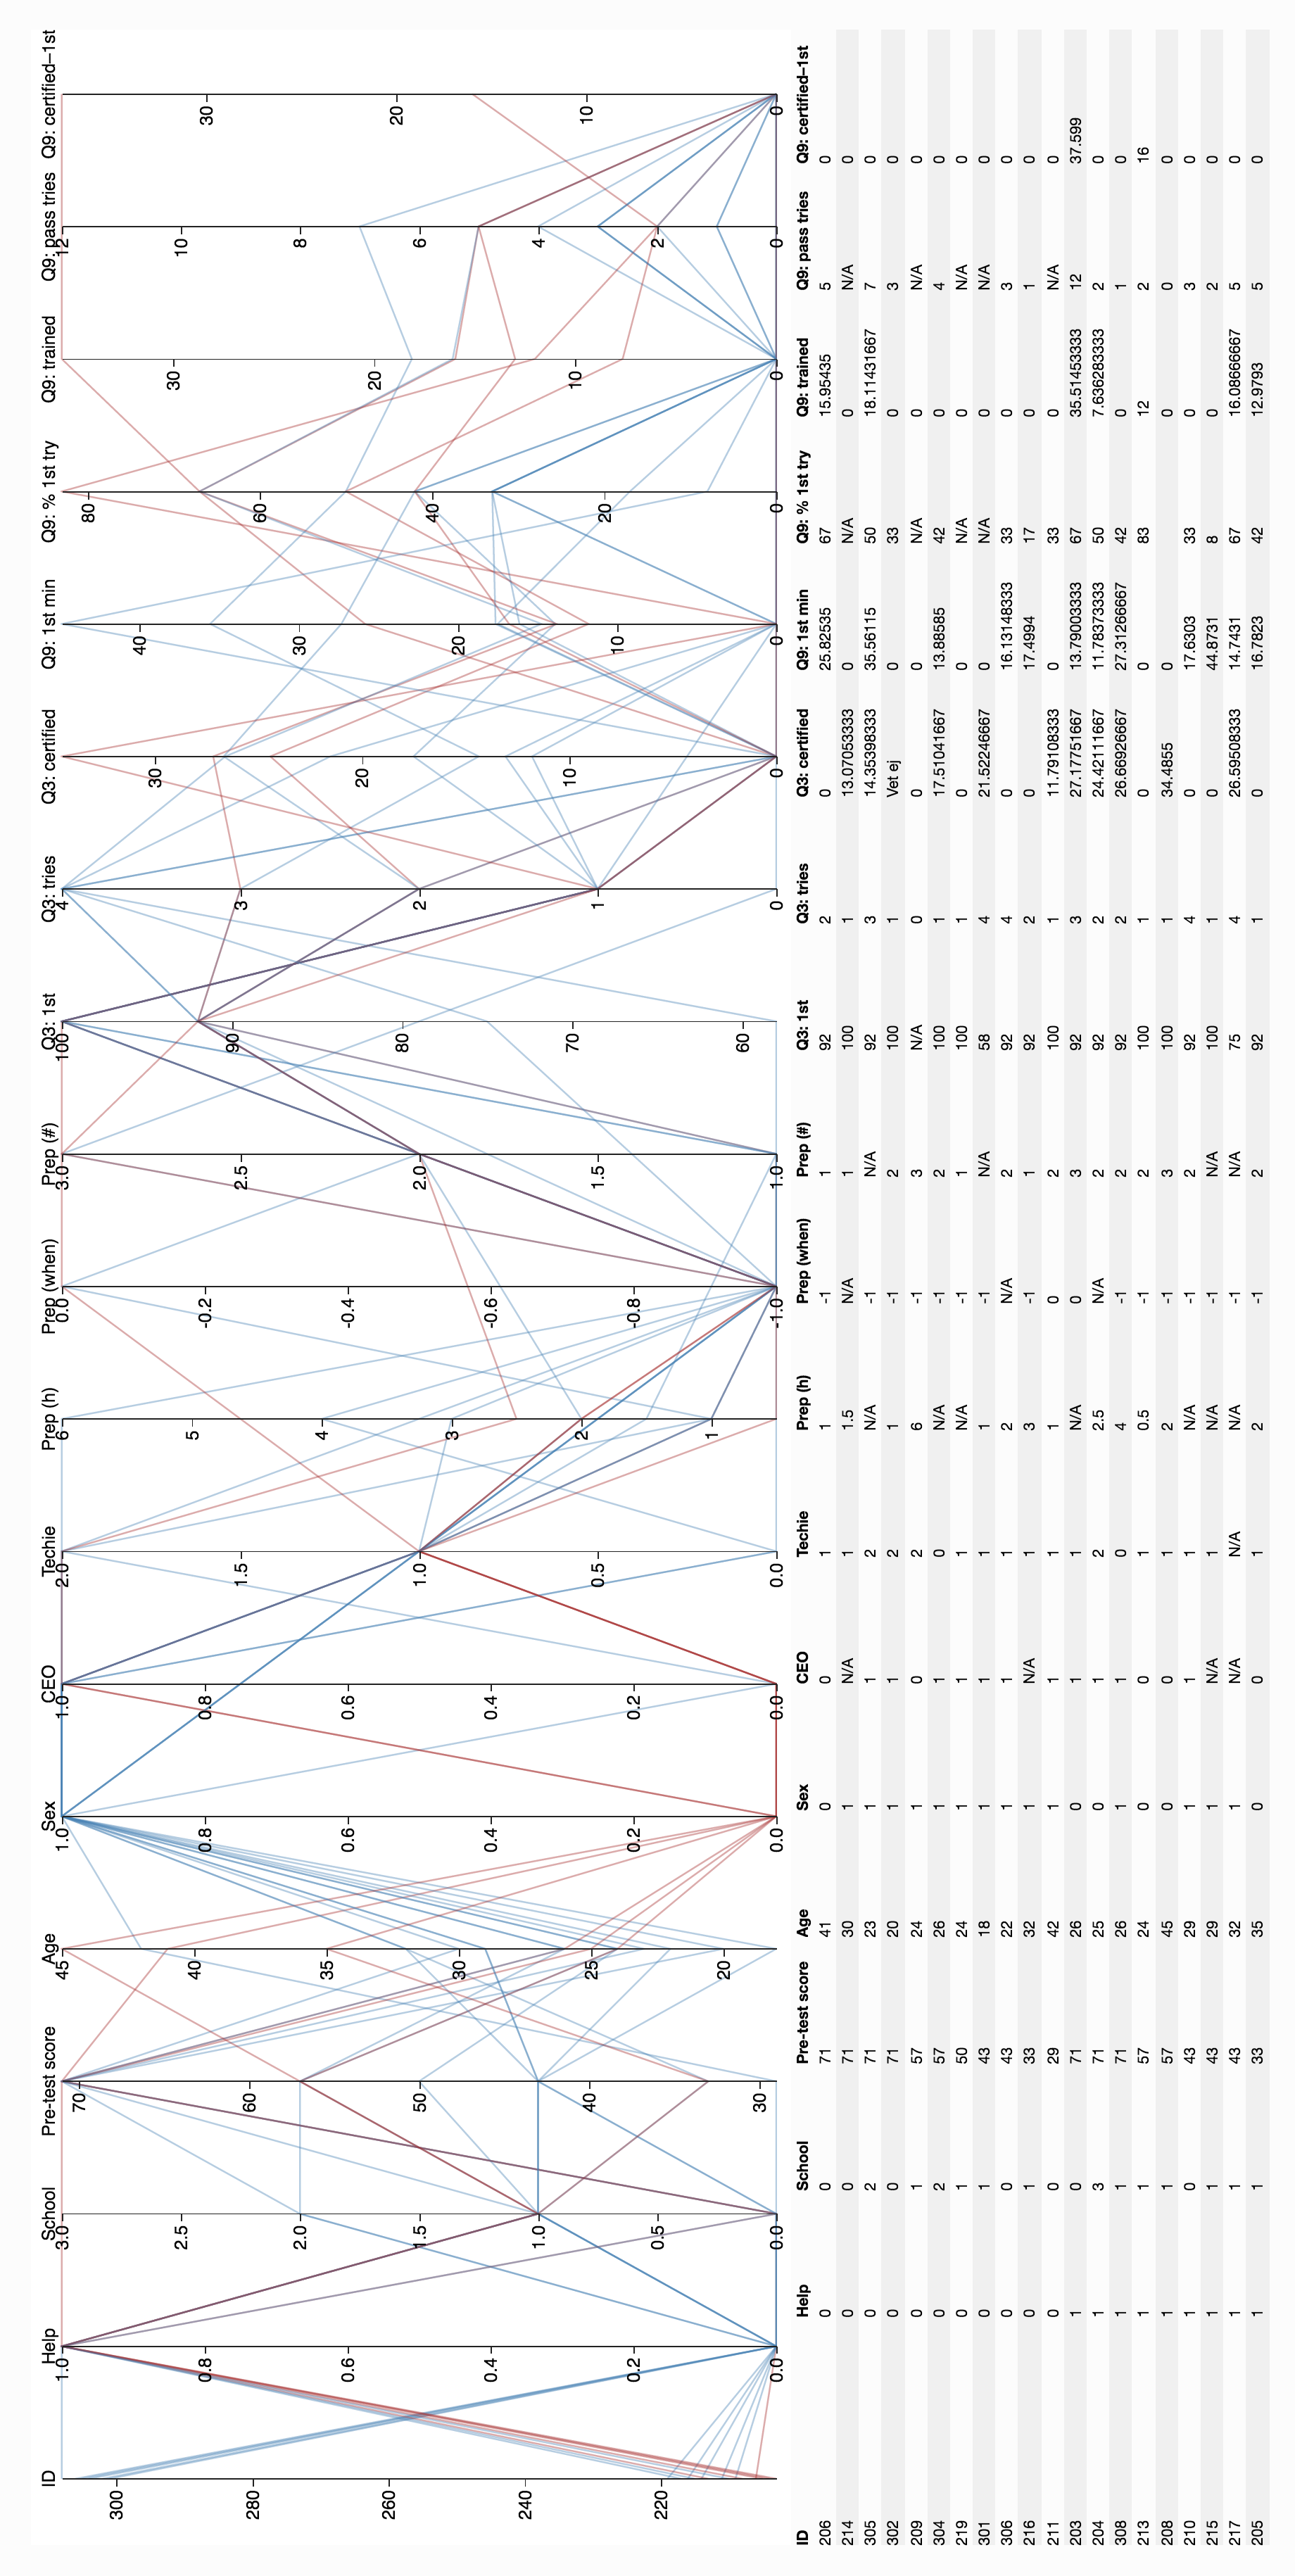
\includegraphics[width=0.7\textwidth]{analysis/parallellCoordinates3.png}
    \caption{The quiz results from iteration 4 shown in an interactive parallel coordinates visualization. The visualization is available on \url{http://marcusnygren.github.io/youngdrive-parallel-coordinates/}.}
    \label{fig:parallellCoordinates3}
\end{figure}

\clearpage

%* 1/6 Youth mentors had brought manual, compared with 8/14 CBTs
%* There are no female Youth Mentors (i.e. 100\% male Youth Mentors)
%* All of the YM's run their own businesses, compared with 5/10 for CBTs

%* Seemingly no difference CBT vs. YM in when prepares for session
%* All YM prepares 2 times for session, while CBT can train also 3 or 1 time)

%* 13/14 CBTs gjorde quiz 3 try 1, 6/6 YM's
Following the lines from column "ID" (for Coach ID), you can compare the difference in performance between Youth Mentors (301-308) and CBTs (201-220). Between quiz 3 and 9, there is no unison difference. In quiz 9 however, the Youth Mentors are top performers compared to CBTs, which goes in line with the project leaders opinion in the field that Youth Mentors are slightly better in the field than the CBTs. This could be explained also by that Youth Mentors only teach YoungDrive, while the CBTs also teaches other programs. It is important to note that there is nothing statistically significant to draw confident conclusions. Further research needs to be made, as a connection between how a coach performs in the field versus the app is valuable. %CBT 6/14 st certifierade, YM 4/6 st

%Quiz 9 (rött=CBT:
%* 6 CBTs gör ej Q9 try 1, 2 YM gör ej
%* YM är top performers på Q9 try 1 jämfört med CBTs
%* endast 1 YM klarade däremot träningen, medan
%* YM's är bättre på quiz 9 try 1 än CBTs
%* Det är endast 1/7 som klarade quiz 9 training som är Youth Mentor
%* Antal försök man gjorde är likvärdigt, förutom en YM som hade 12 försök (och klarade quiz)

%If the app is indeed an indicator if the coach performs well, the data shows that female coaches should be hired for YoungDrive.

The results shows that the ideal coach, according to the quiz app, would be a woman, both in contrast and in unison with the literature mentioned in section \ref{entrepreneurship-education}. In figure \ref{fig:parallellCoordinates3} it can be seen that the female coaches (red lines) on average has better scores than the male coaches (blue lines), in spite of having less formal education. Further, she prepares more, is more aware of her own knowledge and has a better study technique, respecting the app feedback for meta-cognition and meta-memory. More than average, for example in quiz 9, the women have a higher lowest threshold, and a much higher record, than the men. two people were fast enough to get certified on the final quiz before the app evaluation ended, see figure \ref{fig:quiz9pl}. Both were women. Apart from gender, these coaches had higher quiz results, faster learning, and more honesty in "Are you sure?" than the others. Today, the balance between male and female coaches is reversed from what the data says: in Zambia only men have been hired, and in the data collection for Uganda, only 30\% (6/14) were women.

%\textbf{Certified quiz 9}
Other social characteristics on the two coaches that passed the certification for coach quiz 9 is that were that both were CBTs (not youth mentors), and were in the middle of the age groups (24 and 26 years old). Regarding performance, they had a good pre-test score (57\% or 71\%), had top scores on quiz 3 try 1 and 9 try 1. Also, both of them used the manual, they looked at themselves as medium-skilled using a smartphone, and they prepared many times per youth session (2 or 3 times). In figure \ref{fig:quiz9pl}, a more detailed explanation is given. What didn't seem to matter for top performance, was number of tries for passing the training of quiz 9 (one coach did 2 tries on quiz 9, the other 12 tries), or time to pass training quiz 9 (35.5 minutes on the slowest versus 12 minutes on the fastest). Neither did it seem to matter when they prepared their session (1 did preparations the same day, 1 the day before). Regarding social characteristics, one had a business, one didn't, and their school level were both low.

\begin{figure}[h]
    \centering
    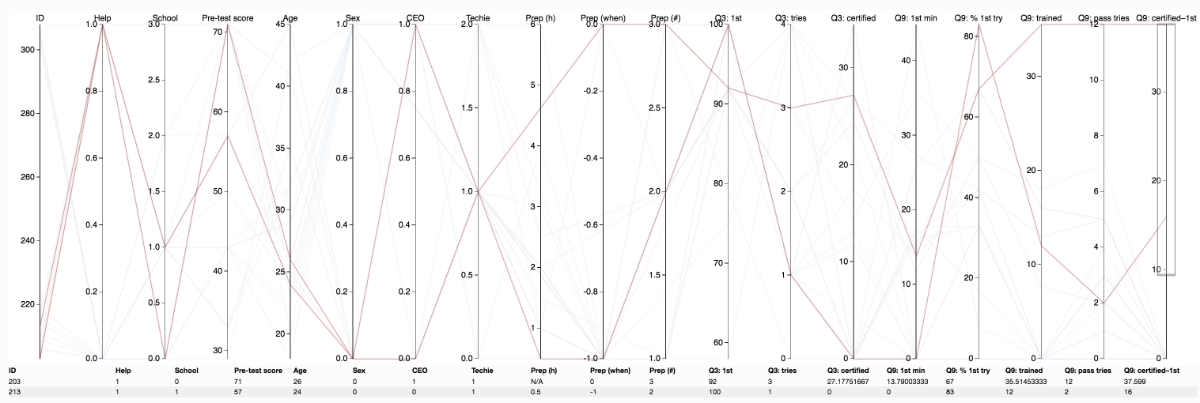
\includegraphics[width=1.0\textwidth]{analysis/paralellCoordinatesWomen.png}
    \caption{The parallel coordinates visualization showing the characteristics of the two coaches that passed the quiz 9 certification. They were both CBTs, they could both could consult the manuals, they had a low education, while still having higher pre-test scores that the average. They were relatively young and were both women (in minority). One had a company and one did not. The one that inserted how she prepared for session, said she prepared the day before (versus doing it the same day), on three occations. Regarding quiz results, they both had a high score on try 1 of quiz 3 "Financial literacy" (1 or 0 errors), just like the majority, and it took them 1 or 3 tries to pass the training. For the coach where time is recorded for getting certified, it took her 27 minutes to pass the quiz (higher than the average). On quiz 9, it took 13 minutes to get 67\%, the other coach (time not known) scoring 83\%. While the coach with 83\% passed the training in only 12 minutes and 2 tries, it was the coach taking 35 minutes to take 12 tries that could afterwards get all of the answers correct in the Certification.}
    \label{fig:quiz9pl}
\end{figure}

Finally, it is interesting to observe the differences (and lack thereof) between the test group and reference group, by following the lines from the second column, "Help", of figure \ref{fig:parallellCoordinates3}. In the test group ("Help" = 1), the paper manuals could be read before improving on the quiz results (not during the actual test) The the reference group ("Help" = 0) were only allowed to observe the right answers within the app, from the score board. In quiz 3, where almost all coaches had 92\% or 100\% immediately, there is no difference observable. However, in quiz 9, the hardest quiz, 5/7 that passed the training were in control group A, and 2/2 that passed the certification were in control group A. An explanation could be that the large amount of questions made the correct answers hard to memorize versus actually learning, or that the ones with manuals felt more supported or motivated because of the extra support. While these findings could be true for a larger sample, further research needs to be done. The same methods of data analysis are increasingly relevant with a larger data set, and there seems to be correlations and tendencies worth looking further into.

%\subsection{Conclusions}

\todo{Add everything from the mindmap}

In three months time, an app was developed with precision to the needs and context of the end users. The design has been heavily influenced by the end users, from day 1 of the project, in conjunction with relevant research, and in balance to stakeholder goals and considerations, and supervisor advice.

The results shows that the ideal coach, according to the quiz app, would be a woman, since she has better knowledge in spite of having less formal education. She prepares more, is more aware of her own knowledge and has a better study technique, respecting the app feedback for meta-cognition and meta-memory. This can be seen by higher quiz results, faster learning, and more honesty in "Are you sure?".

It could be that first-time smartphone users have a disadvantage with the app, since they will not learn as fast as experienced users. The interactions shows however, that at the second session, almost all of the coaches felt intermediate instead of beginners, using the smartphone and the YoungDrive app. The quiz data verifies this, with no direct correlation between technical skills and quiz results.

The final version of the app shows users can get 100\% on quiz results much faster that the previous version, where the score board had been improved. Since the target group in Zambia and Uganda was different, it is hard to say if it went faster getting 100\% with the possibility of repeating only the wrong questions, asking "Are you sure?", and providing individual feedback. The qualitative study does show however, that 100\% thought the feedback was good for learning, and that they appreciate the app.

The data shows that being honest and deliberate during the training increases the likelihood that a coach can get 100\% without faults, and has truly learned. Further, when a coach has passed the certificaiton, they do feel more confident about teaching the topic, since assessment of "Am I ready?" can happen already before the session, and they feel the quiz has been a fair way to measure their knowledge in the topic.


For Discussion, Conclusion and Future Work, see the coming chapters.

%\section{Qualitative Data}
%
%  Here the results from the qualitative data for iteration 1, 2, %3 and 4 are shown.
%
%  \subsection{Qualitative data}

\subsubsection{Entrepreneurship education considerations}
Throught early interviews with YoungDrive staff, it is clear that YoungDrive's entrepreneurship education methodology goes hand in hand with the presented theory. It's mottos are: "Dream big, start small", "Learning by doing" and "We have fun!" \citep{youngdrive}.

Both in regards to designing for the users and for the above reason, the app should be a complement to YoundDrive's existing training material and the structure of the program.

A challenging part of the work is that YoungDrive consists of both the practical skills of the entrepreneur, theoretical material of running a business, and an entrepreneurial mindset. Therefore, both how to assess knowledge, and build habits, needs to be examined.

\subsubsection{Understanding the coach situation}

A CBT can be responsible for from 7 up to 12 different youth groups in different programs, and such a high number places huge demands on the CBT.

Even if there are only 7 groups, being behind on schedule or not being confident, can be very demanding.

\textbf{Stayover at Patrick:} På morgonen visade Patrick mig hur han jobbar med deras tomt, var det odlas ris, och andra råvaror, deras djur, deras story från Syd-Sudan, till Kampala, till hyddan här i Tororo, och hans värderingar.

Efter en ungdomssession nästföljande dag besökte vi och hälsade kort på en av de 2 CBT:s vi har session med idag. Sedan hade jag och Patrick den obligatoriska review av ungdoms-sessionen, och jag bjöd honom på middag. Kl. 19 ringde hans fru (som har börjat få tecken av malaria) och skyndade hem.

Nästa ungdomssession fick jag besöka en annan CBT. Vi var tidiga. Sedan började jag prata med henne, och fick bra tillfälle att intervjua henne och även förklara för henne vad jag gjorde där. Det blev underligt att förklara för henne: Patrick påminde, när jag tabbat mig, att “Marcus, du måste förklara för X vad en app är”. Så hon fick låna min mobil, och jag förklarade att app var kort för applikation, och att för varje applikation har ett eget syfte, t.ex. ta foton. Jag bad henne klicka, svårt, råkade klicka åt henne, men sedan lät jag henne göra. Efter hon sett att det hon såg i skärmen var det hon såg på riktigt, blev hon jätteglad och började fundera vad hon skulle fota. Hon reste sig och gick runt hörnet, och jag följde efter. Hon fotade, efter att noggrannt tänkt igenom, att hon fotade buskarna med frukt. Sedan sade jag hon kunde fortsätta fota, och då tog hon ett litet runt hus utanför.


\subsubsection{Different kind of coaches}

The interviews with CBTs, PLs and stakeholders led to the realization that different coaches handles this differently well.

Depending on the situation, e.g. you are not confident, or you are falling behind with the schedule, you can be in one of these need groups.

\begin{itemize}
  \item The ideal coach
  \item The realistic coach
  \item The challenged coach
\end{itemize}

It was discovered, that coach confidence comes largely from being able to have good youth sessions.

\subsubsection{A good youth session}

For having a good youth session, these are the most important attributes:

\begin{itemize}
  \item Correct information
  \item Correct structure
  \item Time management
  \item Fun atmosphere
\end{itemize}

The fact that the coach knows they have these qualities, leads to self confidence from the coach. This in turn, leads to better meetings with the youth.

\subsubsection{The room for a digital solution}

It is definitely a problem that so extremely few have smartphones.

This needs to be designed for. Either, I build only for the use case of having an app tailored for the coach training, where the donated devices can be used.

Alternatively, I design only for the users that does have a smartphone, and count that more will get smartphones in the future.

Thirdly, I can use a SMS tool, not building an app but an SMS-based service, which also could be an app. Such tools exists, and are compatible with multiple-choice questions, like VOTO Mobile.

%  \subsection{Qualitative data}

\subsubsection{Design workshop \#1 in Zambia}

The result was fantastic, in the sense that it gave me an unbiased look at what the coaches expected from the app, what functionality wasn't important, and into their technical preferences.

The designs and insights gained were used throughout the week to further improve the app I had actually started creating, and gave great insights to who the coaches were and their thinking. \todo{Add image here}

\subsubsection{The desire perspective}

Insight: "The app could be used on my spare time". This is particularly true, about the bonus quizzes that were produced during the week.

Insight: \textit{Coach:} "I'll buy one" (a smartphone), \textit{Response from other coaches: } "Whoa!"

\subsubsection{The utility perspective}

Ideation: "The app should have notes, not only quesitions"

\subsubsection{The usability perspective}

Low resolution screens, made the text be barely visible. This showed, that the app needed to be tested on a lot of different devices. This is particularly true, as on day 1, the coaches did not know how to zoom, which could cause accident refreshs, frustration or confusion.

The app needs to work offline! To be online on the phone is too expensive for the coaches, and too unrealiable to give a satisfactory experience. Also, during testing, relying on internet can cause a lot of problems, especially if the teacher is alone.

\subsubsection{The learning perspective}

    The coaches had surprisingly high results, and at day 3 they wished harder questions when asked.

    We responded by having harder questions, e.g. by introducing similar answers, and testing 4 alternatives instead of 3. This was appreciated.

    The following analysis could be done:

    \subsubsection{Doing a pre-quiz: good for learning}
    When asked about what they thought about doing "Graduation" as a pre-quiz (before the session), 10/10 said they liked doing the quiz before, and that it benefited their learning during the session.

    When asked why it helped, these were the results:

    \begin{itemize}
    \item "During session, it is easier to follow" - 10 (100\%)
    \item "Giving the paper manuals before, scanning headings and pictures etc, would not help" - 10 (100\%)
    \end{itemize}

    It was also tested to work in group or individually. The ones who answered, said that you learned more individually (3/3), and more fun doing it together (3/3). Doing it together, was enjoyable as it was "Very easy because of using different minds" and "We can collaborate to do better".

    \subsubsection{Doing a post-quiz: Spaced versus massed learning}
    In "Goal setting", quotes were "I thought it was fun and challenging to do the quiz immediately afterwards", with another coach commenting "The mind was still fresh".

    When asked on timing preference, 10/10 said it would be more fun to do the quiz immediately afterwards, not at the end of the day. The motivation, seemed to be that it was easier.

    9/10, said they wanted to do the quiz afterwards. The outlier, said it would be better for learning doing it later.

    After this comment, this was the distribution:

    \begin{itemize}
    \item 3/10 wants to do the quiz both before and after a session
    \item 1/10 wants to do the quiz before and at the end of the day
    \item 7/10 wants to do the quiz only immediately afterwards
    \item 10/10 wants to do the quiz immediately afterwards, and then again at the end of the day
    \item 7/10 wants to do the quiz immediately afterwards, and then a joined quiz with other topics at the end of the day
    \end{itemize}

\subsubsection{The teacher perspective}

  \textbf{Low scores}
  The 9/19 shows the relevancy of the quiz, as Josefina did not think she would have discovered that the coach was lagging behind otherwise.

  In the data, it was observable that the coach had done well together with others, but 3/7 when done individually.

  Josefina said about the 9/19: "This is where a control group would be beneficial". "He is often passive during open questions, but active during the team exercises."

  The question we needed to ask ourselves, was: "Does this imply he is a good or bad coach?".

  \textbf{What would hinder Josefina from using the app}

  Josefina says: "Not doing data collection digitally works whenever they are 10 - but not with bigger numbers than that."

  According to the final interview with Josefina, she does not wish the app to replace her. She enjoys teaching, thinks she has an important role, and suggests the app to be designed to support her and the coaches, not replace her.

  \textbf{Acceptance criteria}

  If you have a high score, you are ready. If not, you need to redo the quiz.

  If you are 8/10 or lower, you are in the red zone. If lower than 10/10, they are not ready, the motivation being that what they don't know, they will teach in an improper way: affecting hundreds of youth. This is why Josefina thinks they should need all of the answers correct.

  \textbf{Testing Correct Structure, Time Management and Fun Atmosphere}
  Josefina informs that Correct Structure, Time Management and Fun Atmosphere would be the most valuable to test after a youth session. She also notes, that \textit{some} aseessment could be made via the app before a session. Because of the reason that this thesis does not focus on after-session-evaluation, Correct Information is primary to improving on the other factors, which are secondary.

\subsubsection{The developer perspective}

  \begin{itemize}
    \item Bugs was a big hindrance to functionality, and a lot (both high-dose, and high-scale) of testing is very important
    \item Simpler design than I thought (KISS) was sufficient
  \end{itemize}

\subsubsection{Bonus results: Testing the app on Kampala university student}
The app was tested on a university student from Makarere University.

The university student from Makarere University scored 100\% correct, in spite of not having any entrepreneurship training. This showed that guessing was possible, or that the quizzes were too easy.

%  \subsection{Qualitative data}

  %What the observations said

  \subsubsection{Observations from Kampala test}
  The entrepreneurship student in Kampala, informed the following changes:

  Instead of "Become certified", he would be more motivated by unlocking the opportunity to apply the skills.

  "Improve" should be renamed "Try again", because it is more intuitive.

  His overall opinion on the app was:

  "Can you give me the link, because I'd love to do more of this. I think it's amazing."

  \subsubsection{Verified relevancy of seperating Training and Certification}
  When asked for an opinion, Josefina answered: "I like the idea that when the coaches have answered all of the questions correctly, they can consilidate the knowledge by the certification test, when the coach should get 100\% correct on their first try."

  \subsubsection{Field visits}

  The first thought was to use Gold/Silver/Bronze in the Training mode, and "Are you sure?" in the Certification mode. User tests showed that the other way around was better.

  \subsubsection{Big app test}
  \textbf{Learning: } The app test simulated the app being used to assess preparedness for a youth session. They clearly showed evidence between the difference between designing for Assessment and Learning:

  Given a coach having prepared for their youth session on week 9, and then only scoring 5/10, what should happen? In a similar way, what should happen if 9/10 correct answers?

  For the coach training, the assessment was okay, since Josefina could pick up and give feedback.

  Before a youth session, leaving the coach there is not viable. If the coach has 9/10, that coach should not only be let be, and especially if the score has been 5/10.

  Feedback was that one user did not want to press "Improve", until having read the manual. The motivation was: "Not because that is what the info says, but because I can learn more from the manual, about more than what the questions says."

  This is indeed the preferred behaviour from Josefina, and the app should continue to encourage only using the app training or certification mode after having prepared via the manual. This way, the app is still assessment, but it is "learning by thinking", with feedback.

%  \subsection{Iteration \#4}

Everyone now thought the app was good and easy to use.

With the Plan Tororo staff, it was shown how important the certification mode was: even though one group had 100\% on their first try, and a person had 1 wrong answer, the person with 1 wrong answer got 100\% on the certification, while the 100\% group had 1 wrong answer.

It is therefore determined, that when all of the answers can be answered correctly, after having gotten all answers correct once, that the knowledge is reliable - this is deliberate practice.

%
%\section{Quantitative Data}
%
%  Here the results from the quantitative data for iteration 1, 2, %3 and 4 are shown.
%
%  \subsection{Iteration \#1}

    %What the data said

    \subsubsection{Results from the coaches}

    \subsubsection{Observable trends from the coaches}

%  \subsection{Quantative data}

    %What the data said

    \subsubsection{Results from the coaches}

    \subsubsection{Day 2}
    Most coaches prefer tablet: 5 prefer tablet, 2 smartphone, and 2 computer.

    \subsubsection{Day 3}
    iOS no longer allows uncertified app install from computer: you need to have paid a license even for unreleased apps, being a "Trusted developer". This stops the app from being able to be installed on all the iOS devices, so that only the web version can be used.

    Thus, only the web app was tested from Wednesday and onwards.

    This was a problems, as the app regurly crashed at refresh because of low internet capacity.

    Sometimes, it was neeed to go to the other office where there was wifi, to refresh the webpage, and go back to the location. This of course would not work for Josefina.

    \subsubsection{Day 4}
    Tested using the quiz before the session.  Using the quiz before the session increases learning, slightly decreases fun of the session, according to coaches. It is "Fun and encouraging".

    \subsubsection{Day 5}
    On day 5, the schedule was:

    \begin{itemize}
      \item "Goal setting" part 2
      \item App test: "Goal setting" after-quiz and "Graduation" pre-quiz.
      \item "Graduation"
    \end{itemize}

    In "Goal setting", one coach were an outlier to the other high results, scoring 9/19 answers correct.

    \subsubsection{Results from workshop \#2}

    During this workshop, the focus was to examine what builds confidence among the coaches. The following clusters could be determined: "I believe in myself" (3 coaches), "I believe in God" (2 coaches), "I am well prepared" (4 coaches) and "I am certified" (1 coach). \todo{Lägg till bild här}

    \subsubsection{Bonus results: Testing the app on refugee innovations}
    Back in Uganda, a test was done with refugee innovators, at the Humanitarian Innovation Jam.

    The test with the refugee innovatiors were surprisingly intriguing and successful.

    It was found that refugee innovators says they would have a great need for such an app.

%  \subsection{Iteration \#3}

    %What the data said

    \subsubsection{Observable trends from the coaches}

     \textbf{Usability: } The most notable thing from the app test, was that the app was not user friendly at all for 1st-time smartphone users. There were a lot of bugs, e.g. resizing of the font size for each new question. This forced some coaches to try to zoom on the devices, even if they did not know how. This could in turn cause refresh of the web page, and sometimes there was no Internet available. Thus, the data can not be fully reliable.

  This was the first time true frustration was shown. Out of 23 respondents, 7 rated the app easy, 11 medium, and 6 hard. This was not viable.

    \textbf{Related to mobile experience}
    Before the quiz started, the coaches were asked to raise their hand if they felt proficient with using a smart phone. 8 out of 23 said yes.

    After the quiz, 16 said they were proficient (25\% increase), while 5 said low proficiency, and 2 said no (we don't yet feel proficient, still fear).

    \textbf{Field tests}
    During field tests, 3 CBTs were visited, to further observe usage of the app after having prepared a youth session.

    Some things were notable from the interactions with John:
    \begin{itemize}
    \item "Are you sure?" is understood intuitively (you can't progress without answering), but some coaches deliberately answer "Yes" even if they are not sure.
    \item Idea to highlight different words of similar answers, to increase speed
    \item In summary, if wrong, show the other alternatives either way, not only the wrong answer
    \end{itemize}

    It was also here, that it was first observed that this is a light version of both deliberate practice and perceptual exposure. It is just that the app as of now is quite inefficient, especially in terms of speed.

    \todo{Add idea for future work: Show how a persons correctness level has increased over time}

    From the interactions with Juliet, this was discovered:

    \begin{itemize}
    \item Idea for future work: "Go to participant manual" within the app
    \item If correct and unsure, she says "I still feel good". "Include it in wrong, because maybe I was still guessing". (This later informed the Certification quiz-insight)
    \item Change button to "Become certified", to increase likelihood to press the button. As of now, it was not obvious.
    \end{itemize}

    When she did get certified, she said "I feel good". When asked why, she said: "They have appreciated what I have done".

    \textbf{"Are you ready?" app test}
    The next day, the three CBTs gathered at the Plan International office to do an app test on the hardest quiz.

    \todo{Add results}

%  \subsection{Quantative data}

    %What the data said

    \subsubsection{Results from the coaches}

    \todo{Add table from Google Sheets}

    % Christine och Patrick berättade senare att i regel presterar Young Mentor lite bättre än CBT, enligt deras rakningar. (från iteratoin 1 - stämde detta?)

    Relevans av att testa financial literacy: "Precis som med förra gruppen, verkar ekonomin vara det svåraste att förstå (dolda utgifter, hur gå med vinst), som youth." (från iteration 1)

    \subsubsection{Data observations}

% Important to be objective
% En diskussion om hur resultaten kan användas i praktiken är också i de flesta fall belysande och relevant i rapporter

% https://liu.se/ias/kontakta-oss?l=en

In this section, the conclusions from the different group characteristics are presented.

Early observations from the pre-test data was that a surprising number of cells were left blank. One user had not done the pre-test, where some had left questions unanswered (most commonly "Do you own a company?" (should have used the word "business"), plus "Hours of preperation" and "Occations for a youth session" (there is a tendency this might be because they were not proud of their answers, because of correlations with low quiz results).

Missing cells was not as obvious with the app results, were users could not progress in a quiz without answering both the question and the confidence. However, none of the passed quiz 9 certification answers had been submitted. Thus, it was needed to add these from the manual recordings, which had been used as a backup in case anything like this would happen.


There were a number of quick insights that could be drawn before the parallell coordinates visualization: there was a surprisingly low number of answers where the user answered the question without confidence. Also, more users had started a quiz without finishing it than anticipated. Finally, a lot of users had done quizes that were not Topic quiz 3 and Coach quiz 9, which might indicate high interest (if they did more than 2 quizes) or confusion (if they did not do 3 or 9, but they did do other quizes) during the app evaluation. This meant that on some aspects, there were less data than anticipated, (which was troublesome, as there were already few data points), and some aspects where there was more data than anticipated (that were overlooked).

First-hand insights before the parallell coordinates were that there was a strong corrolation between pre-quiz results and quiz 9 try 1 (slightly visible also in quiz 3 try 1, but with more outliers). Also, with manuals there was a higher probability to finishing quiz 9 training + certification.

\subsubsection{Statistical analysis}
Statistical analysis unfortunately showed that none of the results were statistically significant to be notable using linear regression, or any of the other statistical methods detailed in the methodical framework.

\subsubsection{Parallel coordinates visualization}
The interactive parallel coordinates visualization could give many more insights, more faster than the static presentations in Google Sheets.

\textbf{Youth mentor (brun), 6 st vs. CBT (blå), 14 st}
* Youth mentors has higher school level than CBT's
* 1/6 Youth mentors had brought manual, compared with 8/14 CBT's
* Only 1 CBT has above 2 (1 st 3) on School, while YM have (2st 0, 1 2st, 2 2st)
* Inverse correlation: CBT old, YM young
* There are no female Youth Mentors (i.e. 100\% male Youth Mentors)
* All of the YM's run their own businesses, compared with 5/10 for CBT's
* Only CBT's said they didn't feel comfortable with smartphone (2 st) - because of age?
* Seemingly no difference CBT vs. YM in when prepares for session
* All YM prepares 2 times for session, while CBT can train also 3 or 1 time)
* 13/14 CBT's gjorde quiz 3 try 1, 6/6 YM's
* YM's och CBT's presterar lika på quiz 3 try 1
* CBT 6/14 st certifierade, YM 4/6 st

Quiz 9 (rött=CBT:
* 6 CBT's gör ej Q9 try 1, 2 YM gör ej
* YM är top performers på Q9 try 1 jämfört med CBT's
* endast 1 YM klarade däremot träningen, medan

* YM's är bättre på quiz 9 try 1 än CBT's
* Det är endast 1/7 som klarade quiz 9 training som är Youth Mentor
* Antal försök man gjorde är likvärdigt, förutom en YM som hade 12 försök (och klarade quiz)
* Det var endast 2 st som klarade certifieringen, och båda dessa var YM och kvinnliga

\textbf{Women}

It is clear from the data that women:
* Have lower education level than the men
* Spread results on the pre-test (probably because of school level)
* Half of them are around 25 years old, half spread out (up until 45 years old)
* 2/6 har eget företag
* Det är bara 1 som ej preppar alls
* 1 st som endast preppar 1 gång, alla andra preppar 2 gånger (3 st) eller 3 gånger (2 st)
* Alla hade max 1 fel på quiz 3 på första försöket!
* De som ej hade rätt, tog det bara 2:a (1 person) eller 3:e försöket (1 person)

* 3/6 gjorde certifieringen - kolla upp: började de?

* Alla förutom 1 tjej gjorde svåraste quizet. De hade minst 42\%! Varav 2 st hade 67\%, 1 hade 50, 1 hade 42, och 1 hade 83

* Quiz 9 tjejerna hade mycket högre lägstanivå () än killarna (, och mycket högre högstanivå än killarna () - tiden är jämförbar, med svag tendens snabbare tjejer
* Av de som hade 50\% på 1:a försöket, gick det betydligt snabbare för tjejerna än killarna att jobba igenom quizet - tyder på att tjejerna är säkrare på materialet än tjejerna - dessutom är det bara 2 killar som fick över 50\% på första försöket
* Om du kollar tvärtom, så är det bara 1 tjej som fick under 50\% på första försöket, medan det var 8 killar
* Quiz 3 syns ej lika tydlig skillnad (OBS: kolla vilken fråga de flesta hade fel på, och kolla om det skiljer sig mellan killar och tjejer)
* Skolnivå verkar oberende på hur quizen blir, om man kollar quiz 9
* Tjejer, antal försök quiz 9 hade de 2 (2 st), 5 (2st, 12 (1st) försök innan de klarade - bland killarna var det 5 (1st) och 7 (1st). Men sedan så var det 0 av killarna som blev certified, men 2 tjejer (de som gjorde på 12 försök och 2 försäk). Att antal försök skiljde sig mellan 2 och 12, men ändå klarar det, berättar att antal försök kanske ej korrelerar. Den på 12 försök hade 70\% på försök, och jobbade igen de 12 försöken väldigt snabbt.
* Den andra tjejen som klarade certifikation quiz 9 klarade 83\% försök 1, (hade tillgång till hjälp), klarade träningen sedan på 2 försök.

Slutsats:
* Anställ bara tjejer. De har högre kunskap och förbereder sig mer, trots lägre skolutbildning.

\textbf{Use of participant and coach manuals}

Användande av appen:
* Vi hittade ingen korrelation quiz-resultat 9 första försöket om man fick hjälp eller inte, antagligen pga att man ej använder manualen före

\textbf{Certified quiz 9}
Only two people were fast enough to get certified on the final quiz before the app evaluation ended.

Characteristics were:
* Both of them used the manual
* Both of them were CBT's, not youth mentors
* Both were women
* They were 24 or 26 years old
* They had a good pre-test score (57\% or 71\%)
* They had top scores (1st place and 2nd place (shared with one other)) on quiz 9 try 1
* They had high scores on quiz 3 try 1 (100\% and 92\%
* They prepared many times per youth session (2 or 3 times)

What didn't seem to matter:
* Number of tries quiz 9 (12 vs 2 on Q9)
* Time to pass training quiz 9 (35.5, slowest vs 12 minutes, below average)
* When day trained (1 trained same day, 1 trained the day before)
* One had a business, one didn't
* School level (1 S?, one S lower)

Other:
* They were medium skilled on using a smartphone


%
%\section{Insights}
%
%  \subsection{Iteration \#1}

\subsubsection{Motivation of app}
The scope of the app is to examine and strengthen the entrepreneurship the student already has. One important goal is to give good feedback.

The users are already motivated. Thus, I can follow Sierra's advise designing for the compelling context.

My compelling context is that I want to help you become an even better coach.

The better user point of view: don’t just make a better coach training app - make a better user of coach training material.

For me, this means:

"Given a teaching situation among the youth group, a great coach can teach an entrepreneurship topic more consistent with what the coach material said."

"Given a question in the app, a great coach will get the right answer more often, and increasingly leverage the correct answer to their coach situation."

\subsubsection{Entrepreneurship education considerations}
The YoungDrive's entrepreneurship education methodology goes hand in hand with the presented theory. It's mottos are: "Dream big, start small", "Learning by doing" and "We have fun!" \cite{youngdrive}.

Both in regards to designing for the users and for the above reason, the app should be a complement to YoundDrive's existing training material and the structure of the program.

A challenging part of the work is that YoungDrive consists of both the practical skills of the entrepreneur, theoretical material of running a business, and an entrepreneurial mindset. Therefore, both how to assess knowledge, and build habits, needs to be examined.

%  \subsection{Iteration \#2}

\subsubsection{Insights}

The app works for assessment!

  Using the quiz before the session increases learning, slightly decreases fun of the session, according to coaches

  Fun and encouraging

  \begin{itemize}
    \item The app works for assessment!
    \item Good for learning for the coaches
    \item A good indicator for Josefina
    \item A great way to scale the YoungDrive training in the future, both for online coach-training and the physical training
  \end{itemize}

After the meeting with the partner and expert group, the following was concluded from iteration \#2:

\begin{itemize}
\item The app is only working on assessment now, not for learning
\item The need for a field app still feels relevant (especially for sessions long since the coach training)
\item The potential for YoungDrive having online coach training is huge
\end{itemize}

Determine:
\begin{itemize}
  \item Focus for the next iteration: design quiz app for learning, focus on field app (CI, CS, TM, FA), and design having an app that works stand-alone from the YD coach training in mind.
\end{itemize}

Discussing the importance of self-reflection after a youth session with Josefina, led to asking more of such questions in coach quizzes.

Josefina: “I have a problem: there is no way I can control them how they have prepared themselves for a youth session."

An app could be used, either before you start planning (to guide what you need to study the most on), or after you think you are ready (so you can assess and improve).

\subsubsection{Bonus results: Testing the app outside the YoungDrive context}
Back in Uganda, a test was done with refugee innovators, at the Humanitarian Innovation Jam.

Also, the app was tested on a university student from Makarere University

The test with the refugee innovatiors were surprisingly intriguing and successful.

It was found that refugee innovators says they would have a great need for such an app.

The university student from Makarere University scored 100\% correct, in spite of not having any entrepreneurship training. This showed that guessing was possible, or that the quizzes were too easy.

\subsubsection{Findings}

Test with university student scored 100\% correct, means that common sense can go a long way, and that the results can't be 100\% trustworthy, and that multiple-choice questions has serious issues - this, we already knew during and before the coach training - but it needs to be taken care of

The app would be great and could actually work outside the physical coach training - with revision, be stand-alone, even being able to distribute online.

Now there are observable evidence for what the interactions from Iteration 1 showed:

\begin{itemize}
\item The purpose of the coach training should be to prepare the coach in having great youth sessions
\item Therefore, this is what the quizzess should assess
\item What it really means being a good YoungDrive coach, is having good youth sessions
\item Josefina would have liked to be able to stop coaches from having taught, if they do not have 90-100 \% correct information on the subject
\item Today, Josefina can not assess this. This means that some coaches, are teaching incorrect information to hundreds of youth.
\item Here, the quiz has a very good need to fill.
\end{itemize}

With all of these findings in summary, it can be concluded that an app for coach training, and an app to use before a youth session, could be the same app, since the purpose of preparing the coach to be great with its youth session is the same.

From the interviews, it was learned that while it \textit{may} be technically possible, the teacher desires the app support her, not replace her.

%  \subsection{Iteration \#3}

  The app works for assessment!

  \begin{itemize}
    \item The app works for assessment!
    \item Good for learning for the coaches
    \item A good indicator for Josefina
    \item A great way to scale the YoungDrive training in the future, both for online coach-training and the physical training
  \end{itemize}

%  \subsection{Iteration \#4}




%\begin{chapter-appendix}

%\section{Proof-Appendix}
%
Det här är en appendix-del av det aktuella kapitlet.

%\end{chapter-appendix}

%\chapter{Analysis}

% Important to be objective
% En diskussion om hur resultaten kan användas i praktiken är också i de flesta fall belysande och relevant i rapporter

% https://liu.se/ias/kontakta-oss?l=en

In this chapter, each step of the visualization pipeline is presented, allowing analyzing the data. Then, conclusions are presented.

The Visualization Pipeline describes the process of generating an image from the data: \cite{timo-ropinski-liu}

\begin{enumerate}
\item Data acquisition ($\,\to\,$data are given)
\item Data enhancement ($\,\to\,$ data are processed)
\item Visualization mapping ($\,\to\,$ data are mapped to for example a geometry)
\item Rendering (3D->2D) ($\,\to\,$ images generated)
\end{enumerate}

% Timo Ropinski, Scientific Visualization Group, Linköping University, TNM067 - Scientific Visualization, 9/12/2014)
% https://drive.google.com/drive/u/0/folders/0BzlK1PD8EE75bHIxcXRQNWpRMm8

\section{Data acquisition}

This section presents how data was acquired.

\subsection{App usage}
The app pushes data to server when online (it saves quiz start, and quiz finish).

The server receives JSON data, stored in a MongoDB database.

Each data point is saved in a database called Results, with the signed in user (from the Users database).

It was desired to store the data in Google Sheets, thus it was necessary to convert the JSON format into a Google Sheets-readable format, like CSV.

Multiple approaches were tried, and the Google Chrome extension called Magic Json by agaze\_dev\_team (last updated October 29, 2015) %https://chrome.google.com/webstore/detail/magic-json/cajifcebjiflndefndbnoeenjpiiiagm?hl=en
was the one that worked without problems. \cite{agaze}.

\subsection{Pre-study}

The Pre-study data was done by manually recording the paper-submitted pre-study evaluation form from the coaches, into Google Sheets.

\section{Data enhancement}

This section presents how the data was processed, to enable visualization mapping.

\subsection{App usage}
To make the data easier to work with, the columns were reordered, and made sortable and filterable.

Some columns were given conditional formatting, so it would be easier to spot irregularities.

\todo{Lägg till bild "results-colored.png" (finns på skrivbordet)}

After this, some observations could be made. For example, there was a surprisingly low number of answers where the user answered the question without confidence. Also, more users had started a quiz without finishing it than anticipated. Finally, a lot of users had done quizes that were not Topic quiz 3 and Coach quiz 9, which might indicate high interest (if they did more than 2 quizes) or confusion (if they did not do 3 or 9, but they did do other quizes) during the app evaluation. This meant that on some aspects, there were less data than anticipated, (which was troublesome, as there were already few data points), and some aspects where there was more data than anticipated (that were overlooked)

\subsection{Pre-study}
To see differences in answers more clearly, the data from the pre-study was made sortable and filterable. Then, the data was resampeled for each column that hade numerable (sortable) data in text instead of numbers, so e.g. "The day before" was changed to -1 and "The same day" to 0. In a similar way, school level was divided into four different groups, from 0 to 3, where 0 meant secondary, year unknown, 1 meant lower secondary, 2 meant upper secondary, and 3 meant tertiary.

After this, each column was given conditional formats using a color scale, using Google Sheets built-in functionality. This gave a visual way to quickly get a overview of the pre-test data.

Observations from the data was that a surprising number of cells were left blank. One user had not done the pre-test, where some had left questions unanswered (most commonly "Do you own a company?" (should have used the word "business"), plus "Hours of preperation" and "Occations for a youth session" (there is a tendency this might be because they were not proud of their answers, because of correlations with low quiz results).

Missing cells was not as obvious with the app results, were users could not progress in a quiz without answering both the question and the confidence. However, none of the passed quiz 9 certification answers had been submitted. Thus, it was needed to add these from the manual recordings, which had been used as a backup in case anything like this would happen.

\subsection{Summary of app results}

To compare the test results with the pre-test results, it was clear that it would not be viable to test every dimension against every dimension.

Instead, since goals of the app evaluation had been predefined in the following way, the quiz results were summarized so that the following could be derived:

\begin{itemize}
\item \% correct 1st try
\item number of tries until 100\%
\item number of tries until 100\% in 1 try
\end{itemize}

These could be calculated by having columns for:

\begin{itemize}
  \item Quiz 3
  \begin{itemize}
    \item Start time training
    \item \% correct 1st try
    \item number of tries until 100\% in 1 try
    \item Time difference start to end time certification
  \end{itemize}
  \item Quiz 9
  \begin{itemize}
    \item Start time training
    \item \% correct 1st try
    \item Time difference start to end 1st try
    \item Time difference start to passed training
    \item Time difference 1st try to certified
  \end{itemize}
\end{itemize}

Then, to see trends, I again added color scales. With ordinal values, a sequential color scheme is used (e.g. fastest time, from green to red), and with nominal values (like if they are female or male) where there is no right value, a qualitative color scheme is used. Now, it was easier to spot outliers and trends.

First-hand observations were that there was a strong corrolation between pre-quiz results and quiz 9 try 1 (slightly visible also in quiz 3 try 1, but with more outliers). Also, with manuals there was a higher probability to finishing quiz 9 training + certification. More

\subsubsection{Comparing the pre-test and results summary sheets}

I joined the two sheets, meaning I had created a multiple-variate data set (serveral dimensions that I needed to compare with several dimensions).

I met with my university supervisors, so they could further support me in how to properly analyze the data.

It was clear that analysis in Google Sheets could only go so far. It was greatly helpful to sort by multiple columns (e.g. first by Manual?, then by School level, then by Quiz 3). However, it took a long time to filter the data on multiple parameters, and the work became tedious. It was not viable to discover the data using this approach.

Meeting with the supervisors, they started by comparing the means on the pre-quiz results with the two control groups. Since they showed similar results, the two control groups were comparable.

Then, we calculated the means from the other columns based on e.g. "Manual?", gender, school category, high app quiz result, etc.

A multivariate analyzation software or a visualization was suggested to discover the data in less time.

It was hard for us to determine a suitable multivariate analysis software suitable when having so few data points. Principle Component Analysis or Cohen's kappa would not be suitable, or to do Linear correlation on all dimensions.

After discussion with other Master thesis students working with large amounts of data (one from KTS and one from MT), parallel coordinates was suggested. It would allow me to very quickly filter the data, find correlations, and distinguish outliers and common characteristics.

To learn how to analyse the data, Une-terre (2012) was consulted. % http://une-terre.blogspot.se/2012/09/parallel-coordinates-read-out-patterns.html
He writes "||-coords are a data visualisation which allow you to "read out" the relationships and trends between your dimensions. Positive relationship (correlation), negative relationship (invert), or no relationship (random)."

\subsection{Visualization mapping}
The goal with visualization mapping is to generate renderable data.

Thus, I added a new spreadsheet, specific for visualizing the data.

I deleted columns that would serve no visual purpose (e.g. timestamps), gave all cells data values (even N/A when undefined), deleting users that did not have data, and shortened the column names so they would fit on the screen.

The data was then exported from the Google Sheet into CSV.

\subsection{Rendering}

For rendering, the JavaScript library D3.js was chosen. It supports data-driven documents for visualizing data with HTML, SVG and CSS. It supports both JSON and CSV data.

A visual framework for multidimensional detectives for D3.js was found, called "Parcoords.js", written by Chang Kai (2012).
% https://syntagmatic.github.io/parallel-coordinates/
% Chang, K. (2012). Parallel Coordinates toolkit : Parcoords.js 0.1. Parallel Coordinates toolkit. Retrieved September 8, 2012, from http://syntagmatic.github.com/parallel-coordinates/
% Kosara, R. (2010, May 13). Parallel Coordinates. Eagereyes.org. Retrieved September 8, 2012, from http://eagereyes.org/techniques/parallel-coordinates
% Tricaud, S. (2008). Picviz: finding a needle in a haystack. Proceedings WASL, San Diego. Retrieved from http://www.usenix.org/events/wasl08/tech/full_papers/tricaud/tricaud.pdf

The example code from "Linking with a Data Table" provided the basis for the rendering. It would be a great benefit to bee able to see both a parallel coordinates visualization, and to see the same values present in the Google Sheet. %https://syntagmatic.github.io/parallel-coordinates/examples/table.html

I replaced the example CSV file with the exported Google Sheets data in CSV.

Eventually, I also changed the colors, and added to the example the toolkit's functionality to drag the axes titles around to reorder the dimensions, since the goal was to quickly compare and find correlations.

\todo{Lägg till bild på parallella koordinater-visualiseringen}

\section{Findings}

In this section, the conclusions from the different group characteristics are presented.

\subsection{Correlations}

\textbf{Youth mentor (brun), 6 st vs. CBT (blå), 14 st}
* Youth mentors has higher school level than CBT's
* 1/6 Youth mentors had brought manual, compared with 8/14 CBT's
* Only 1 CBT has above 2 (1 st 3) on School, while YM have (2st 0, 1 2st, 2 2st)
* Inverse correlation: CBT old, YM young
* There are no female Youth Mentors (i.e. 100\% male Youth Mentors)
* All of the YM's run their own businesses, compared with 5/10 for CBT's
* Only CBT's said they didn't feel comfortable with smartphone (2 st) - because of age?
* Seemingly no difference CBT vs. YM in when prepares for session
* All YM prepares 2 times for session, while CBT can train also 3 or 1 time)
* 13/14 CBT's gjorde quiz 3 try 1, 6/6 YM's
* YM's och CBT's presterar lika på quiz 3 try 1
* CBT 6/14 st certifierade, YM 4/6 st

Quiz 9 (rött=CBT:
* 6 CBT's gör ej Q9 try 1, 2 YM gör ej
* YM är top performers på Q9 try 1 jämfört med CBT's
* endast 1 YM klarade däremot träningen, medan

* YM's är bättre på quiz 9 try 1 än CBT's
* Det är endast 1/7 som klarade quiz 9 training som är Youth Mentor
* Antal försök man gjorde är likvärdigt, förutom en YM som hade 12 försök (och klarade quiz)
* Det var endast 2 st som klarade certifieringen, och båda dessa var YM och kvinnliga

\subsection{Women}

It is clear from the data that women:
* Have lower education level than the men
* Spread results on the pre-test (probably because of school level)
* Half of them are around 25 years old, half spread out (up until 45 years old)
* 2/6 har eget företag
* Det är bara 1 som ej preppar alls
* 1 st som endast preppar 1 gång, alla andra preppar 2 gånger (3 st) eller 3 gånger (2 st)
* Alla hade max 1 fel på quiz 3 på första försöket!
* De som ej hade rätt, tog det bara 2:a (1 person) eller 3:e försöket (1 person)

* 3/6 gjorde certifieringen - kolla upp: började de?

* Alla förutom 1 tjej gjorde svåraste quizet. De hade minst 42\%! Varav 2 st hade 67\%, 1 hade 50, 1 hade 42, och 1 hade 83

* Quiz 9 tjejerna hade mycket högre lägstanivå () än killarna (, och mycket högre högstanivå än killarna () - tiden är jämförbar, med svag tendens snabbare tjejer
* Av de som hade 50\% på 1:a försöket, gick det betydligt snabbare för tjejerna än killarna att jobba igenom quizet - tyder på att tjejerna är säkrare på materialet än tjejerna - dessutom är det bara 2 killar som fick över 50\% på första försöket
* Om du kollar tvärtom, så är det bara 1 tjej som fick under 50\% på första försöket, medan det var 8 killar
* Quiz 3 syns ej lika tydlig skillnad (OBS: kolla vilken fråga de flesta hade fel på, och kolla om det skiljer sig mellan killar och tjejer)
* Skolnivå verkar oberende på hur quizen blir, om man kollar quiz 9
* Tjejer, antal försök quiz 9 hade de 2 (2 st), 5 (2st, 12 (1st) försök innan de klarade - bland killarna var det 5 (1st) och 7 (1st). Men sedan så var det 0 av killarna som blev certified, men 2 tjejer (de som gjorde på 12 försök och 2 försäk). Att antal försök skiljde sig mellan 2 och 12, men ändå klarar det, berättar att antal försök kanske ej korrelerar. Den på 12 försök hade 70\% på försök, och jobbade igen de 12 försöken väldigt snabbt.
* Den andra tjejen som klarade certifikation quiz 9 klarade 83\% försök 1, (hade tillgång till hjälp), klarade träningen sedan på 2 försök.

Slutsats:
* Anställ bara tjejer. De har högre kunskap och förbereder sig mer, trots lägre skolutbildning.

\subsection{Use of participant and coach manuals}

Användande av appen:
* Vi hittade ingen korrelation quiz-resultat 9 första försöket om man fick hjälp eller inte, antagligen pga att man ej använder manualen före

\subsection{Certified quiz 9}
Only two people were fast enough to get certified on the final quiz before the app evaluation ended.

Characteristics were:
* Both of them used the manual
* Both of them were CBT's, not youth mentors
* Both were women
* They were 24 or 26 years old
* They had a good pre-test score (57\% or 71\%)
* They had top scores (1st place and 2nd place (shared with one other)) on quiz 9 try 1
* They had high scores on quiz 3 try 1 (100\% and 92\%
* They prepared many times per youth session (2 or 3 times)

What didn't seem to matter:
* Number of tries quiz 9 (12 vs 2 on Q9)
* Time to pass training quiz 9 (35.5, slowest vs 12 minutes, below average)
* When day trained (1 trained same day, 1 trained the day before)
* One had a business, one didn't
* School level (1 S?, one S lower)

Other:
* They were medium skilled on using a smartphone

\chapter{Discussion}\label{cha:discussion}

% %Ingen rapport kan göra anspråk på att ha löst problemen inom ett område på ett uttömmande sätt. Därför är det viktigt att visa på vilket sätt du själv eller  andra kan använda dina resultat i andra studier i framtiden. Den avslutande  diskussionen blir till sin karaktär mer subjektiv, men se till att du inte  spekulerar alltför vilt.

%\todo{Alla källor jag nämner, de behöver jag egentligen diskutera i Discussion-delen. Då börjar jag vrända och vida på saker, och hitta olika tankemönster = Vad som stämmer och inte stämmer i det jag sett jämfört med teorin}

The discussion section is framed by revisiting the five research questions. For each question, important aspects are considered, often comparing with the literature. This then leads to the conclusions of the master thesis, and future work.

%\section{Technical development}
\section{How is the Development Affected by the Technical Possibilities?}
%\section{What in the development has been affected by the technical possibilities?}

As devices were limited, a goal was to make the app available on as many devices as possible. Creating a hybrid app using web technologies using Meteor made the app available both as a native app on Android and iOS devices, as well as on the web. On the other hand, this is not enough: the pre-evaluation showed that only 3 out of 16 had a smartphone today \cite{youngdrive-statistics}.

As internet is accessible but expensive and often used seldom, the app does not provide rich media or simulations, but focuses instead on creative design possibilities using multiple-choice, also having cognitive load and scaffolding in mind. The interviews and observations from iteration 4 details that the coaches are happy with the user friendliness of the app, and that the training in its current form has high value for the coaches. On the other hand, images could probably be used to lower misconceptions in language, and a future wish of the coaches is to have the manuals accessible via mobile as well, which includes both text and images.

Most of the coaches have been first-time smartphone users. Letting them continuously test and co-create the app has created a tailor-made app from their needs and conditions. It may be surprising how simple design solutions using text and clear visuals can provide rich learning feedback, mentioned by Nocol \cite{nicol}. On the other hand, since it is so tailor-made, it needs to be examined if to make the app work in other countries than Uganda and Zambia, where design and technology preferences might be different.

That the app should work offline, and still be able to push quiz results when it gets online, has been a challenge. It can be hard to find good existing approaches for some technical platforms, but for Meteor plugins such as GroundDB proved very usable, since it is also automatic. In other apps in developing countries sometimes the user decides themselves when to push data, but in this case, quiz results are so small in size that it was unnecessary. This might be reconsidered in the future, for example if answers are no longer solely multiple-choice.

Below, reasons the development was negatively affected by the technical constrains are highlighted.

\subsection{Online Data Collection was Needed Earlier}
To test on all of the coaches in Uganda, it would have been preferable if data collection would have happened via the app instead of manually already in iteration 3, since there would be more than 10 test subjects, which had been the limit in Zambia. This was planned for, but technical implications with Meteor made it delayed. Done manually, not all data was recoded in iteration 3, which made it harder to draw conclusions from the quiz results. Both Lopez \cite{une-terre} and \cite{ropinski} explains how visualization techniques (like parallell coordinates) are more suitable for large data sets. This can be read more about below.

\subsubsection{Problems with Internet Access}
In day 3 of the Zambia coach training in iteration 2, iOS no longer allowed uncertified app installs from computer: you needed to have paid a license even for unreleased apps, being a "Trusted developer". This stopped the app from being able to be installed on all the iOS devices, so that only the web version could be used. Thus, only the web app was tested from Wednesday and onwards. This was a problem, as the app regularly crashed at refresh because of low internet capacity. Sometimes, it was neeed to go to the other office where there was wifi, to refresh the webpage, and go back to the location. This of course would not work for Josefina. While it was positive that these issues were found thanks to testing, valuable time testing the actual functionality of the app was lost, with less feedback for continued development as a result.

\subsection{Backwards Capability Issues} \label{backwards-capability}
Upgrading from version 1.2 to 1.3 during Iteration 3 was a good example of technical limitations. It took a lot of time, but when it was discovered that version 1.2 did not work for old Android devices, the changes needed to be reverted. In another project, new Andorid versions might have been acceptable, but here a "better" version of software was not viable.

Meteor 1.2 had several disadvantages: while it worked for all devices, it did not support React.js Meteor 1.3 was released, which promised a better developer experience, with JavaScript ES6 support, and access to Node Package Manager (npm), plus official support for React.js. In 1.2, only some npm packages had been adapted for Meteor, and tools such as Webpack could not be used.

The downsides was discovered after implementation: there were missing backward compatibility to the older of the Android devices. The backup would be the web version, but at the time of iteration 3, there were no Heroku build-pack for Meteor 1.3, making the website to crash. This was however fixed before iteration 4, which is why Meteor 1.3 was kept.

\subsection{No Time Assigned for Writing Automatic Tests}
The project would have benefited from passing automatic tests before doing user tests. While automatic tests were never written because of time constratints, since iteration 3, beta releases and production releases were seperated into different domains, using Heroku's staging environement, with a different GitHub branch for each new iteration.

Even so, doing automated tests would could have helped finding things that had worked previously but not in a new version, or finding bugs with new functionality like client-server communication. This would have made interactions with coaches more efficient, since the users would have been exposed to an app with less accidental errors.

\subsection{Difficulties Comparing Quiz Results between Iterations}
It would be highly interesting to compare the quiz results between different itreations of the app, to measure how much learning has increased. However, the educational range and knowledge between Zambia and Uganda is too large to draw such conclusions: while all of the Zambia coaches had 100\% correct answers on quiz 3 "Financial literacy" (iteration 2), the same number for Uganda was 91.8\% (iteration 4). This makes further conclusions very hard, more than from informed guesses and observations. See more about this in section \ref{future-work}. How to compare empirically measure learning effectiveness between different countries could be interesting future work.



%\section{Study development}

\section{How is the Design Affected by the Contextual Constraints, e.g. Young Entrepreneurs, Entrepreneurship Education, and Culture?} % such as X, Y, Z, \Å?

  An insight is how quickly the coaches have increased their fluency with using the smartphone and the app. Even though the design at first needs to be very simple, as long as features are introduced slowly and as intuitive, the app could become more complex over time, to the point where no compromises needs to be made.

  When it comes to design constraints in regards to overcoming cultural differences, learning from the expertise of local partners and tech companies can not be overestimated. They have been very willing to share previous mistakes, learnings and successes. This has saved a lot of time, and made the sparse amount of interactions and development time so much more efficient. Also, the value of getting to know the coaches on a first-hand basis has been greatly beneficial. The app has been designed together with them as co-creators, with a developed mutual interest and understanding, having a common goal of creating an app that works for their needs.

  The design was heavily influenced by starting the project with an iteration to truly understand the target group and context, and see the needs before starting thinking about ideas. It was good that this iteration did not have a digital focus, but even questioned if the best way to solve the needs would be an app altogether. Thanks to service design, everything in the app is informed by needs, which is an example of being a thoughtful designer \citep{lowgren} \citep{stickdorn}).

  Service design methodology allowed the design to be embraced by the contextual constraints. Since service design involves looking at the whole context, both the digital context and the physical context, it was possible to understand in what situation the app can be used, and the situation of the people using it.

  When it comes to designing for entrepreneurship, the focus for this thesis was on the educators: both the teacher, and the YoungDrive coaches. This goes in line with the insights from \cite{ruskovaara}, where the teacher seemed to be the main factor for qualitative entrepreneurship education. However, contrary to \cite{ruskovaara}, women did perform better than the male counterparts in the quiz results. Similar results have been found in other developing countries as well: from the pre-test, it is noticed that women puts more work into preparation, even if they have a lower school level. This could be one reason why their results where better.

  More so, the interviews with coaches shows that the app has been fun to use, which was a recommendation from both YoungDrive and the research from \cite{dickson} on recommendations for entrepreneurship education. Secondly, the app has focused on another best practice from \cite{dickson}, which is that the app should develop the competences as a mentor, enabler or coach. This can be noticable by interview answers such as "open's up ones mind" and that it "evaluates my performance" with "how I've understood", "how I'm performing" and that "the feedback is excellent".

  \subsubsection{From Computer Expert into a Digital Service Designer}
  The study method took the project a long way, to the point where research, experiments, and constant improvements could lead to increasingly well-informed decisions.

  New-found skills are acquired within:
  \begin{itemize}
  \item ethnology (getting to know and learn from people in a different culture)
  \item human-centered design
  \item design thinking
  \item service design thinking
  \item interaction design
  \item digital learning
  \item data analysis
  \end{itemize}

  It has placed high psychological pressure and leadership demands as a new designer, to:
  \begin{itemize}
  \item always be in charge of balancing all the different perspectives, with the end user's best in mind
  \item be able to change the planned process when new learnings or opportunities emerge (leading an agile design process)
  \item always implement new functionality from customer needs instead of designer or engineer bias
  \item continually design and run workshops and tests suitable for the target groups
  \end{itemize}

  The reason why this has been especially hard, is that simultaneously to learning design and technological skills, it has been in a different cultural setting than the designer is used to. This has also been extremely rewarding, at the same time exhausting.

  \subsubsection{Having Many People Involved in the Design Process to Adapt to the Contextual Constraints}

  The contextual constraints affected the design in the way that more expertise and guidance was needed than otherwise, from a diverse set of people. Service design research proposes to have a diverse team to build with a holistic perspective \citep{stickdorn}, and this has been followed.

  In the project, working with service design in another culture has been one of the hardest and most exciting challenges. When the interactions for iteration 1 were cancelled the day before the trip because of local elections, experts could empower and affirm that this was not out of the ordinary. A learning was that it is only possible to plan to a certain extent, but then changing the plan in the last second, is needed more than when one's own culture. This support has been very helpful, having several people familiar with working in a different cultural context before.


  To seek out people and situations that were not obvious, gave new insights into the work.  The project partner Plan International, did not only back up the interactions and provide their own expertise, but also allowed interviews with experienced consultants from Grameen Foundation and Designers without Borders. Another examples includes involving Expedition Mondial in the design process, testing the app on university students and refugee innovators and at startup hubs, and involving the local YoungDrive project leaders more than originally thought.

  It was very valuable to combine having a diverse team with the designer having a clear direction and caring for the vision of the product. Otherwise, the product might have ended up in many different directions

  The fact that the end users and stakeholders has been involved from the start, made them feel and have actual ownership of the product. This has many benefits, among others that \textit{everyone} involved is satisfied with the \textit{final} app, since their opinions and expertise has been taken into consideration and implemented. The fact that they can notice this further increases trust, and the the likelihood of them supporting future work, which goes in line with \cite{stickdorn}. To conclude, the design has been affected heavily by the contextual constraints, to the point where the end users are more likely to use the app as they have contributed to making a tailor-made product for themselves.

  \subsubsection{Spending Time in the Real-World Training}
  The original time plan stated that the interactions for Iteration \#2 would have been in Tororo, and that it would not be possible to test the app during coach training whatsoever.

  %Therefore, Iliana Björling from YoungDrive did questions during Iteration \#2 initially for only two sessions, guided by the YoungDrive manuals and Bloom's Taxonomy educational objectives.

  However, during a Skype meeting with YoungDrive project leader Josefina, it was announced that it would be possible to participate in the coach training in Zambia during Iteration \#3.

  A new work plan was created, which would allow travel to Zambia and to develop the app and participate in the YoungDrive coach training together with the coaches.

  Now, it was shown already at Iteration \#2, that if the app would have been created solely by the designer, it would have been assumed necessary with more functionality. The field hackathon, designing and developing together with the users, was fantastic - already for iteration 1, the purpose "Validate the coaches' level of knowledge during their education" could be fulfilled. The two following iterations could not focus on "Train the coaches on distance", and "Certify all staff".

  Also, without the 5 days of the training, questions for each topic would not have needed to be created, and this would then have been a must-have for Future work. %Thus, Josefina gradually created questions for all the days, but because of the lack of time, she did not use Bloom's Taxonomy to analyze the questions against educational objectives.

  The intense training in Zambia gave a lot of time to discuss and interact with the trainer, Josefina Lönn. One important contextual constraint that was noticed, was that Josefina did not want to be replaced, but appreciated having the YoungDrive to the point where the app should not replace her, even if it in the future would benefit YoungDrive in terms of for example monetary reasons. This might not only be personal preference, as \cite{ruskovaara} claims how important the role of the teacher is for effective entrepreneurship education.

  Without visiting the Zambia training, it would have been much harder to focus on the coach training purpose of the app, since the Uganda coach training was already over. A consequence might have been that the app would have been more focused solely on "Train the coaches on distance". This shows that spending time in the real-world context of the situation you are developing for, is very important. - especially when it is unfamiliar to you. This goes in line with the service design principles \citep{stickdorn}.

  \subsection{Having Low Scores on the Quizzes Might Lower Motivation}
  Interestingly from iteration 4, the coaches scoring from 0-53\% on quizzes included two coaches being top performers in Iteration 4, but also the two coaches that did not show up for Iteration 4. Further research could be done, if the difference was on motivation or fixed versus growth mindset. It could be for some, that low quiz results in iteration 3 led to not wanting to use the app any more. The app was designed to be more empowering in iteration 4, but naturally, the app could not be tested on the two coaches that did not show up.


%\section{Learning development}

\section{How can test questions be developed to support entrepreneurship learning?} % Bloom

  The problem identified with multiple-choice questions, regardless if the recommendations by Nicol \cite{nicol} were taken, is that they first could only measure lower-order learning objectives, see figure \ref{fig:revised-bloom}. While entrepreneurial \textit{knowledge} objectives might be considered A-B 1-2, building entrepreneurial \textit{skills} is definitely related to C-D 3-6.

  When assessing the first question sets according to Bloom's revised taxonomy, some characteristics were shown, which guided future creation of questions. Most notably, to reach C-D 3-6 on Bloom, there were some techniques: intelligent multiple-answers could encourage the coach to \textit{evaluate} instead of using process of elminination or encouraging guessing. Putting the coach in a coach scenario (how to act in X situation?), the coach could be tested on a \textit{procedural} and \textit{metacognitive} level to \textit{apply}, \textit{analyse} and \textit{evaluate} skills, and get feedback.

  Previous research by for example Nicol \cite{nicol} had already shown how multiple-choice can be powerful, for example by following the principles in figure \ref{fig:multiple-choice}. The same articles mentions the approach taken with using a confidence-meter similar to "Are you sure?". These recommendations have been utilized.

  Some bad questions have still existed, where coaches did not understand and failed to interpret the question, because too advanced English language was used. This points out the value of testing.

  %What is new in this research, is that 1) the confidence-meter is used for feedback, not only assessment, and 2) multiple-choice questions are formulated in a way that supports higher-learning objectives (see Bloom), like entrepreneurship learning.

  %To achieve 2), Bloom's revised taxonomy was used to identify that the standard multiple-choice format did often practice lower order learning objectives (like Factual/Conceptual or Remember/Understand), which fits for entrepreneurial knowledge, but not for entrepreneurship skills. By constructing questions from real-world situations, multiple-choice questions can test procedural knowledge, and the coach may need to also analyse scenarios. The only limitation, is that the coach can not apply the procedural knowledge in the app, but also in real life. Also, as long as the questions are not constructed by the coach herself, she will not reach the \textit{create} level on the cognitive process dimension.

  %\subsubsection{The benefit of having quizzes for the whole YoungDrive training}

  Regarding testing and improving the quality of questions, the initial plan was that YoungDrive would only produce questions for two YoungDrive training weeks, not all 10. To have questions for all of the weeks have greatly benefited the master thesis, and increased the value of the final product. If not all quizzes would have been developed and tested, this would have been a Future Work.

  From a question assessment, it is shown that all of Bloom's levels can now be reached via the app, but two: \textit{create}, and \textit{apply}. This is because users can not create anything in the app, and because of the multiple answers are shown immediately, they are not encouraged to apply their own thinking to the question, before seeing the alternatives.

  % Kritik
  \subsection{Learning effect}
  To the largest extent, the questions have been praised, in regards to formulation and challenge, which can be seen in figure \ref{fig:learning} and \ref{fig:interactiondesign}.

  The lack of a post-test makes it hard to see if the test questions in the app has a real-world effect. Ideally, the post-test in Uganda would have been to observe coaches having their youth session, and compare their correctness and confidence behaviour when not having used the app. %In Zambia, coaches were observed by Josefina, the teacher, but the results are not comparable since all coaches used the app during the training.

  The lack of data (not least from the pre-quiz), makes it hard to draw reliable conclusions from the data. Regarding the pre-quiz paper submissions, the submissions should have been checked for blanks before handed in. Another mistake was that school level was not always exactly specified, and this means that school level and quiz results might have a stronger correlation that can be shown now.

  Regarding recording test question results, this should have been done manually already in iteration 3. The fact that it was done automatically in the app for iteration 4, made so that more data could be recorded, more reliably, than when the project leaders filled them in by hand whenever a coach raised her hand to say she was finished with a quiz.

  The biggest evidence for a learning effect, is the coaches who had a low score on their first try with a quiz, but after the training could pass the certification test, getting 100\% in 1 try. \todo{Improve this section}


%\section{Learning development}

\section{How does design affect usability and learning done via the app?}

  The quiz design is made with Kathy Sierra's model of deliberate practice in mind. \cite{sierra} Depending on the combination of correct and sure, the coach knowledge for each question is put into three different buckets: "Can't do", "Can do with effort" och "Can do effortlessly". By retaking the "Can't do" questions with Try again, reflecting on the "Can do with effort" questions (for example: correct but unsure), and waiting to test the "Can do effortlessly" questions until the certification, all questions are eventually put into "Can do effortlessly".

  The coach can choose to leave the training without doing the certification quiz, later repeating the test. This is to make the learning self-directed and just-in-time, and to allow the coach to do it's own scaffolding. If the coach uses the app before a youth session, and has a low result, the coach will get feedback as such (for example: "Nice effort, but you still need to practice and prepare yourself even more! How can you do that?").

  The goal is to allow the coach to move knowledge from "Can't do" to "Can do effortlessly" to "Certified" in a pace that suits the coach. This might be neccessary, instead of a one-fits-all solution, as the coaches' preferences are so different.

  The learning goes faster in iteration 4 than in iteration 3, which is most notably shown by the fact that the speed from try 1 into getting 100\% in 1 try has increased. This is largely because usability issues has been addressed, and because design choices has been made that stimulates and makes learning more efficient. Most notably, the score board has been improved to show which questions the coach is correct and sure of ("Can do efforlessly"), unsure but correct on ("Can do with effort"), and were wrong on ("Can't do"). One mistake made, was no not think about reducing cognitive load \cite{sierra} until iteration 4, when usability issues were identified as serious problems in iteration 3.

  The YoungDrive app is the first known application which uses a confidence metric (in this case "Are you sure?") for the student's own sake, and not only assessment, like in the case study detailed by Nicol \cite{nicol}. The effect is reaching meta-cognitive on Bloom's.

  %\subsubsection{Benefits of "Are you sure?"}
  %"Det här kan motverka %traditioner och ”så här vi alltid gjort det” genom att %tvinga en att reflektera över varför inte ens rätta svar %korrelerar med hur empowered du känner dig. Bryter normer, %sätter sig emot lathet och agerar proaktivt för en skarpare %utveckling tillsammans."



  %Lena frågades också om vilken skala jag ska ha på 5, 4 eller %vad jag inte tänkt på, 2-gradig skala. 5 eller 4 är vilket %som enligt literatur, det finns två olika skolor. 2-gradiga %skalan bedömde jag vara bäst, p.g.a. användarvänlighet, tydligt för coacherna

  \subsection{Benefits with confidence level and correctness in combination}
  If a coach is wrong and sure about a lot of questions, it might be the indication that the coach is teaching the wrong information to the youth, which might potentially hurt hundreds of their youth's businesses.
  %Fanns extremt många fördelar med denna, och kom bara fram %till ännu fler efter diskussioner med människor och Lena %Tibell, framför allt hur denna kan förbättra utbildningen %och 1-on-1 coachning, och bli väldigt bra självreflektion %för coachen.

  If the coach is correct but not confident, it could be considered a guess. In Sierra's framework of building expertise, it would be called "Can do with effort". In the app during iteration 3, dampened for iteration 4, there were troubles when coaches passing the training with too many correct guesses, knowledge that were not yet "Can do effortlessly". This meant that they would fail the Certification, because they could not answer reliably, providing the wrong alternative. This in turn meant, that they were put back into training instead of getting a medal, which was not motivating. The conclusion was that the coach should not start the Certification mode before being truly ready.

  One solution could have been that "Improve" would not only include repeating wrong answers, but also answers where the coach had been correct but said "No" on "Are you sure?". However, coaches seldom believed they would be wrong, or at least did not determine it worthwhile to be honest. Some preventative measures were taken to try to make the coach more honest. Unfortunately, for iteration 3, only some coaches took notice of number of tries as an indication that they should pay more attention. For iteration 4, the design had improved by giving coaches minus points for being sure and wrong, but here as well, not everyone payed attention. This goes in-line with research both from deliberate practice being a desirable difficulty (learning being hard might make the coach more likely to want to "cheat", or take an easier route like guessing instead of putting more effort).

  The bigger problem was that the knowledge were not yet reliant, not that coaches were not honest. The solution for iteration 4 was to improve learning in the app, partly by a more personal score board with feedback, which could show the coach which kind of questions she needed to repeat ("Can't do" or "Can do with effort"), but instead of forcing the coach to redo correct guesses ("Can do with effort"), she could reinforce the correct answers by personal feedback. Sierra \cite{sierra} calls this "high pay-off tips", which can be very effective.

  \subsection{Deciding on learning methods}
  There was a lot of work behind choosing the learning design methods in Iteration \#3. The way to progress, was to brainstorm various solution, discuss them with experts, and then create trigger material and test some of these approaches.

  Retaking questions that were wrong ("Try again", called "Imrpove" in iteration 3) was inspired by deliberate practice \cite{sierra}, and is already common in e-learning driver license softwares to learn traffic signs or how to act in various situations.

  Showing the coach how many quiz tries they have done, was inspired by Linköping University's work with the e-learning tool NTA Digital, where they reward students with badges for getting 100\% in few tries. Their goal with this kind of "gamification", is to reward students for studying before taking the test. Similarly, for the training mode, the coach seeing number of tries was a method of studying the correct answers more thoroughly. For the certification, where the coach was supposed to have trained before taking the test, badges worked with the same purpose as NTA Digital, to reward students that had studied properly.

  %In their application, this is so subtle to the user that only performance-driven students might take notice, whereas students that are not motivated by this are not discouraged.

  "Are you sure?" was inspired by a Swedish teacher, and has been used before by others. \cite{nicol} It has then been used to determine if a right answer should award a point or not. Nicol and the pedagogical expert for this thesis, Henrik Marklund, suggested that the teacher had overlooked a learning benefit of this approach: the student reflecting on their own knowledge, which is proved great for learning. This was extended in this thesis where personalised feedback has the goal of the coach getting both confident and correct. In a school situation, this might not be neccessary, but in the YoungDrive context, the purpose of the app was to build both correctness and confidence with the material. To pass the certification after training, getting 100\% without faults, made the coach feel that confidence, at the same time reassuring the teacher that the coach had learned the material.

  After iteration 4 a bonus test was made with Plan Tororo staff, which showed the relevancy of the certification mode: one group that were 100\% correct on the first try, did get 100\% correct on their second try, meaning guesses had been present. On the other hand, a person have 1 wrong answer, passing the training on the second try, did then pass the certification on the first try, with confidence. It can therefore be determined, that when all of the answers are answered correctly, after having gotten all answers correct once, that the coach has both correct information and confident - this is a good example of deliberate practice: the information has gotten reliable.

  Other learning design methods were considered, as previously discussed. It was discussed if multiple-choice answers should be completely abandoned, replaced with flashcards. Challenges were that the coaches had no previous knowledge of typing on a keyboard, and analyzing recorded answers would be too technically demanding. The integration and benefits of flashcards was however discussed in various ways, see Future work.


%\section{Study development}

\section{How can users' feedback be used to inform modifications of the app?}

  The number one time waster, has been spending time building ideas that is not informed by the users' feedback, and not immediately realizing the mistake. Such ideas will not be used, are often not supported by research, or does not fit the context. This is the same finding that Stickdorn has made \cite{stickdorn}, and is a violation from service design principles of making the process user-centered. Luckily, almost all of the work with the master thesis has indeed been user-centered.

  Getting enough feedback to evaluate each component of the app has been important. Enough feedback, means that modifications to the app can be made with confidence. The faster this can happen, the faster the app gets better. This is why the field hackathon, and service mini-sprints, were so beneficial, see \ref{digital-service-design}. It ensured that fast iterations could happen with enough feedback to provide effective modifications and additions. The use of service mini-sprints was so effective that the interactions in Tororo could be expanded with even more days, as long as this is properly planned for.

  As long as the users understand the purpose of the app, and how it should benefit them, they can be part of the creation process, not only the testing. This is an extraordinary opportunity, that should not be underestimated. To involve the users and get to know them, is essential to understand the true needs of the coaches, and can greatly inform modifications of the app.

  The app evaluation shows that not only should users' feedback inform modifications of the app, they should be the \textit{basis} of the app. To do this, this report has provided but one approach, via Digital Service Design. It is also a service design principle, making the process co-creative \cite{stickdorn}.

  The presence of different perspectives (from users, stakeholders, experts, and the designers care for the vision) lead to a holistic view when designing, inline with Stickdorn \cite{stickdorn}. The designer can balance these, as long as the views are present during the whole development process, and not only in the end of the project. For the questionnaire made for iteration 1, stakeholder views were very important. From their views, the questions could be improved and put into context, and lessons were learned which otherwise would not have happened. In iteration 1 it was felt that maybe too much time was spent with stakeholders, almost to the point where the process where no longer user-centered.

  By asking Why-why-why continually, the true needs of the coaches could be gradually exposed. Similarly, by hosting co-creation workshops, the coaches can be part of designing lo-fi app prototypes that addresses these needs. The role of the designer then, becomes putting these ideas into a context, and comparing with best practices and relevant research (in this case, most notably learning design), modifying, developing, and testing. As Löwgren and Stolterman says, the output will not be better than the designer carrying out the process \cite{lowgren}. To embrace the role of a socio-technical expert, more so than the computer expert or political agent, has been one of the enablers for co-creation. Service design thinking and methods, gave a framework to have all of these perspectives in balance and consideration, always with the end user as the most important person.

  %Discuss how user's feedback should be used to inform modifications of the app, compared to what I have done

  %Do this by comparing the results with research, and analyzing the method

  %What research was used to let users' feedback inform modifications of the app?
  %Research recommends when developing an app, that the app is regularly tested with the thought users. Both qualitative and quantitative data can inform modifications.

  %To evaluate usability, the interaction design principles of desirability, utility, usability and pleasurability can be used.

  %To evaluate learning, interviews and comparing pre-test and test results (and ideally also a post-test).


  %When evaluating the app, there are many different frameworks that can be used.

  %Service design takes this one step further, putting the users in the center of the product development, and letting the users be co-creators.



  %Users feedback was analysed in terms of interaction design principles (evaluate desirability, utility, usability and pleasurability), service design methodology (qualitative data analysis) and



\section{Summary}

As of now, the app can not be said to evaluate how good the coaches are with teaching. Neither, it helps them assess their ability to learn (it sure would be valuable for coaches to track their ability to get better and remember, see chapter \ref{cha:future-work} Future Work). The app does however help the coaches to assess their knowledge level and what areas they need to train on.

Moreover, the coaches seems to like the app, which is important. There are tendencies that the app works better for some coaches, especially those who take time to reflect on the feedback given by the app. This speaks for designing the app for different need groups. If motivation and confidence is high, it could indicate them becoming better teachers, but as of know there are no evidence of this more than that the coaches themselves has identified that confidence is important for having a good youth session.

A bonus result is that the app allows also the teacher to assess the knowledge level of the coaches on a day to day basis during the training, giving insight into how well their teaching has been received. The teacher can use this data to understand what they need to repeat the following day, or if adapting their teaching will lead to higher results. Allowing the teacher to analyse their test questions according to Bloom's Revised Taxonomy created awareness of what knowledge level they were assessing the coaches with by their questions, and motivated matching the formulation of a question to the knowledge and cognitive process dimension suitable for the educational objective.

\chapter{Conclusions}\label{cha:conclusion}
% important to relate to the Purpose

% Sätt av ett kort kapitel sist i rapporten till att avrunda och föreslå rikningar för framtida utveckling av arbetet.

In response to the research questions, the master thesis has: %investigate if the work can:

\begin{enumerate}
\item Contributed to the domain of entrepreneurship education in a developing country context
\item Demonstrated how certain technical constraints and design constraints can be overcome in a developing world context
\item Provided methods of investigating usability and learnings with a digital training tool in the real-world entrepreneurship training context
\item Created new methods in service design, when co-designing digital artefacts in a developing country context
\end{enumerate}

Below, these four items are explained in greater detail, tying the report to a close before suggesting future work in the final chapter.

\section{Contribution to the Domain of Entrepreneurship Education in a Developing Country Context}
This research shows that an app can be effectively used during and after training to assess and learn entrepreneurship. Furthermore, the app can also prepare coaches before youth sessions, training them both in entrepreneurship and preparing their lessons.

In \textit{addition}, this has been done in a developing country context, with coaches having no prior smartphone experience. The app is used for coaches in conjunction with a physical entrepreneurship training today, and does not yet address the youth themselves, or replaces the physical training.

However, the research shows that both the teacher and the coaches greatly appreciates the support the app has given them. As entrepreneurship to its nature is practical in many aspects, one finding is how multiple-choice questions can increasingly simulate real situations by meta-cognitive feedback, using design solutions such as asking "Are you sure?", giving personal feedback, and formulating questions as scenarios.

\section{Demonstration of how Certain Technical Constraints and Design Constraints can be Overcome in a Developing World Context} % service design in development environments % Designprocessen, frågeställning 1

In this project, it was decided to design the app \textit{together} with first-time smartphone users. Co-designing the app with the coaches and learning their perspective on overcoming the technical constraints was a valuable methodology.

Apps developed specifically for rural areas has previously been built that has overcome rural areas’ challenges with access to smartphones, internet and electricity. This learning app is designed to consume low battery and internet by not being media-rich but on relying on text. It is also internet-aware by storing app data locally until internet is turned on. Until every coach is equipped with a smartphone, the app has been deliberately designed to work as a compliment to the physical coach training. After the training, it is not mandatory for a coach to use the app to help prepare for a session, even if it would improve youth session quality.

The workshops shows that coaches are willing and enable to pay for devices by micro-loan or utilizing the savings group, if granted access. Today, they have no such means by YoungDrive or the project partner. YoungDrive can cope with using the donated devices during the coach training, but needs to determine on a strategy to enable smartphone access to the coaches. A conclusion is how in many cases creative design can overcome technical constraints, but not always.

%Today coach training usage is able to cope with donated devices, but they are not enough to give every coach a smartphone. The app has proven less effective to use in group than individually. As the app does show a valuable learning effect, it is now up to the client to give incentive and enable coaches to buy, borrow or rent smartphones.

\section{Provided Methods of Investigating Usability and Learnings with a Digital Training Tool in the Real-World Entrepreneurship Training Context} % Utvärdering, frågeställning 2

To investigate usability, observations using think-aloud in the real-world entrepreneurship training context proved the most effective. In big groups, data could give tendencies on common problems that needed to be addressed. In smaller groups, ideas and precise feedback was more common. It helped having a framework to compare usability against, in this case the interaction design principles of desirability, utility, usability and pleasurability \citep{clatworthy}.

To investigate learning in the real-world entrepreneurship training context, literature research and data analysis of quiz results was highly beneficial, but mostly when put into the context of the observations made in the real-world entrepreneurship training context.

Surprisingly often, comparing research and expert opinions with what coaches thought was best for learning, was in unison. When this happens, the self-confidence of the designer can increase, and the designer can be more daring and experimental.

Having much testing and co-creation was a very rewarding approach, as is discussed in section \ref{sec:user-feedback}. To make it truly testable, lo-fi and hi-fi prototypes should be used instead of hypothetical questions. While research before starting to develop is a great start, it was trying different solutions, all based on user advice, expert opinion and research, that gave great results.

\section{Created New Methods in Service Design, when Co-Designing Digital Artefacts in a Developing Country Context}
Short iterations is a challenge, especially when time is sparse and the culture is different than one's own. Often in projects, testing is overlooked. In this project instead, service design helped to look at the users as not only testers, but as co-creators. This is not new in itself, but the creation of Digital Service Design, and methods within this discipline, were new. Examples include service mini-sprints and field hackathons.

Interactions with the coaches always included Service Mini-Sprints (see \ref{mini-sprint}), allowing the most important feedback and insights to be addressed in the app and workshop formats already the next day. This allowed for very effective use of the sparse interactions with the coaches, and there was no need to wait for the next iteration to test the coaches' feedback.

The "field hackathon", in which the app was refined and tested each day of the coach training, was the most rewarding research and development opportunity of the whole master thesis. More than the opportunity to develop the app with the coaches, it had the extra benefit of giving the opportunity to observe the YoungDrive training and understand the coaches.

To use a service design approach when co-creating digital artefacts in a developing country context proved highly effective, and it is recommended that this area is further studied. It does demand bravery of the designer to get to know the users well \citep{lowgren}, and design for their needs and dare to question the client as \cite{stickdorn} encourages. In the end, as this project and \cite{stickdorn} suggests, including both the users and the client will often make them more satisfied with the result, feeling both increased ownership and that the product feels and indeed has been designed from their needs.

\section{Future Work}

The future work section is divided by research question, and proposes additions that would strengthen the app goals (see \ref{purpose}).

\subsection{Research question 1}
\section{How is the Development Affected by the Technical Possibilities?}\label{rq1}

Some of the wished development were too complex to be implemented during the master thesis. Below, it is described what future work is wished in the area.

\subsection{Data Analysis Improvements}
Today, data analysis of quiz results takes a tremendous amount of time, and is not easily accessible or understood by the stakeholders. The data needs to be acquired into Google Sheets, and then needs to be enhanced in several ways to be filterable and visualized. The raw data when inserted into Google Sheets can be seen in figure \ref{unprocessedData}.

\begin{figure}[h]
  \centering
  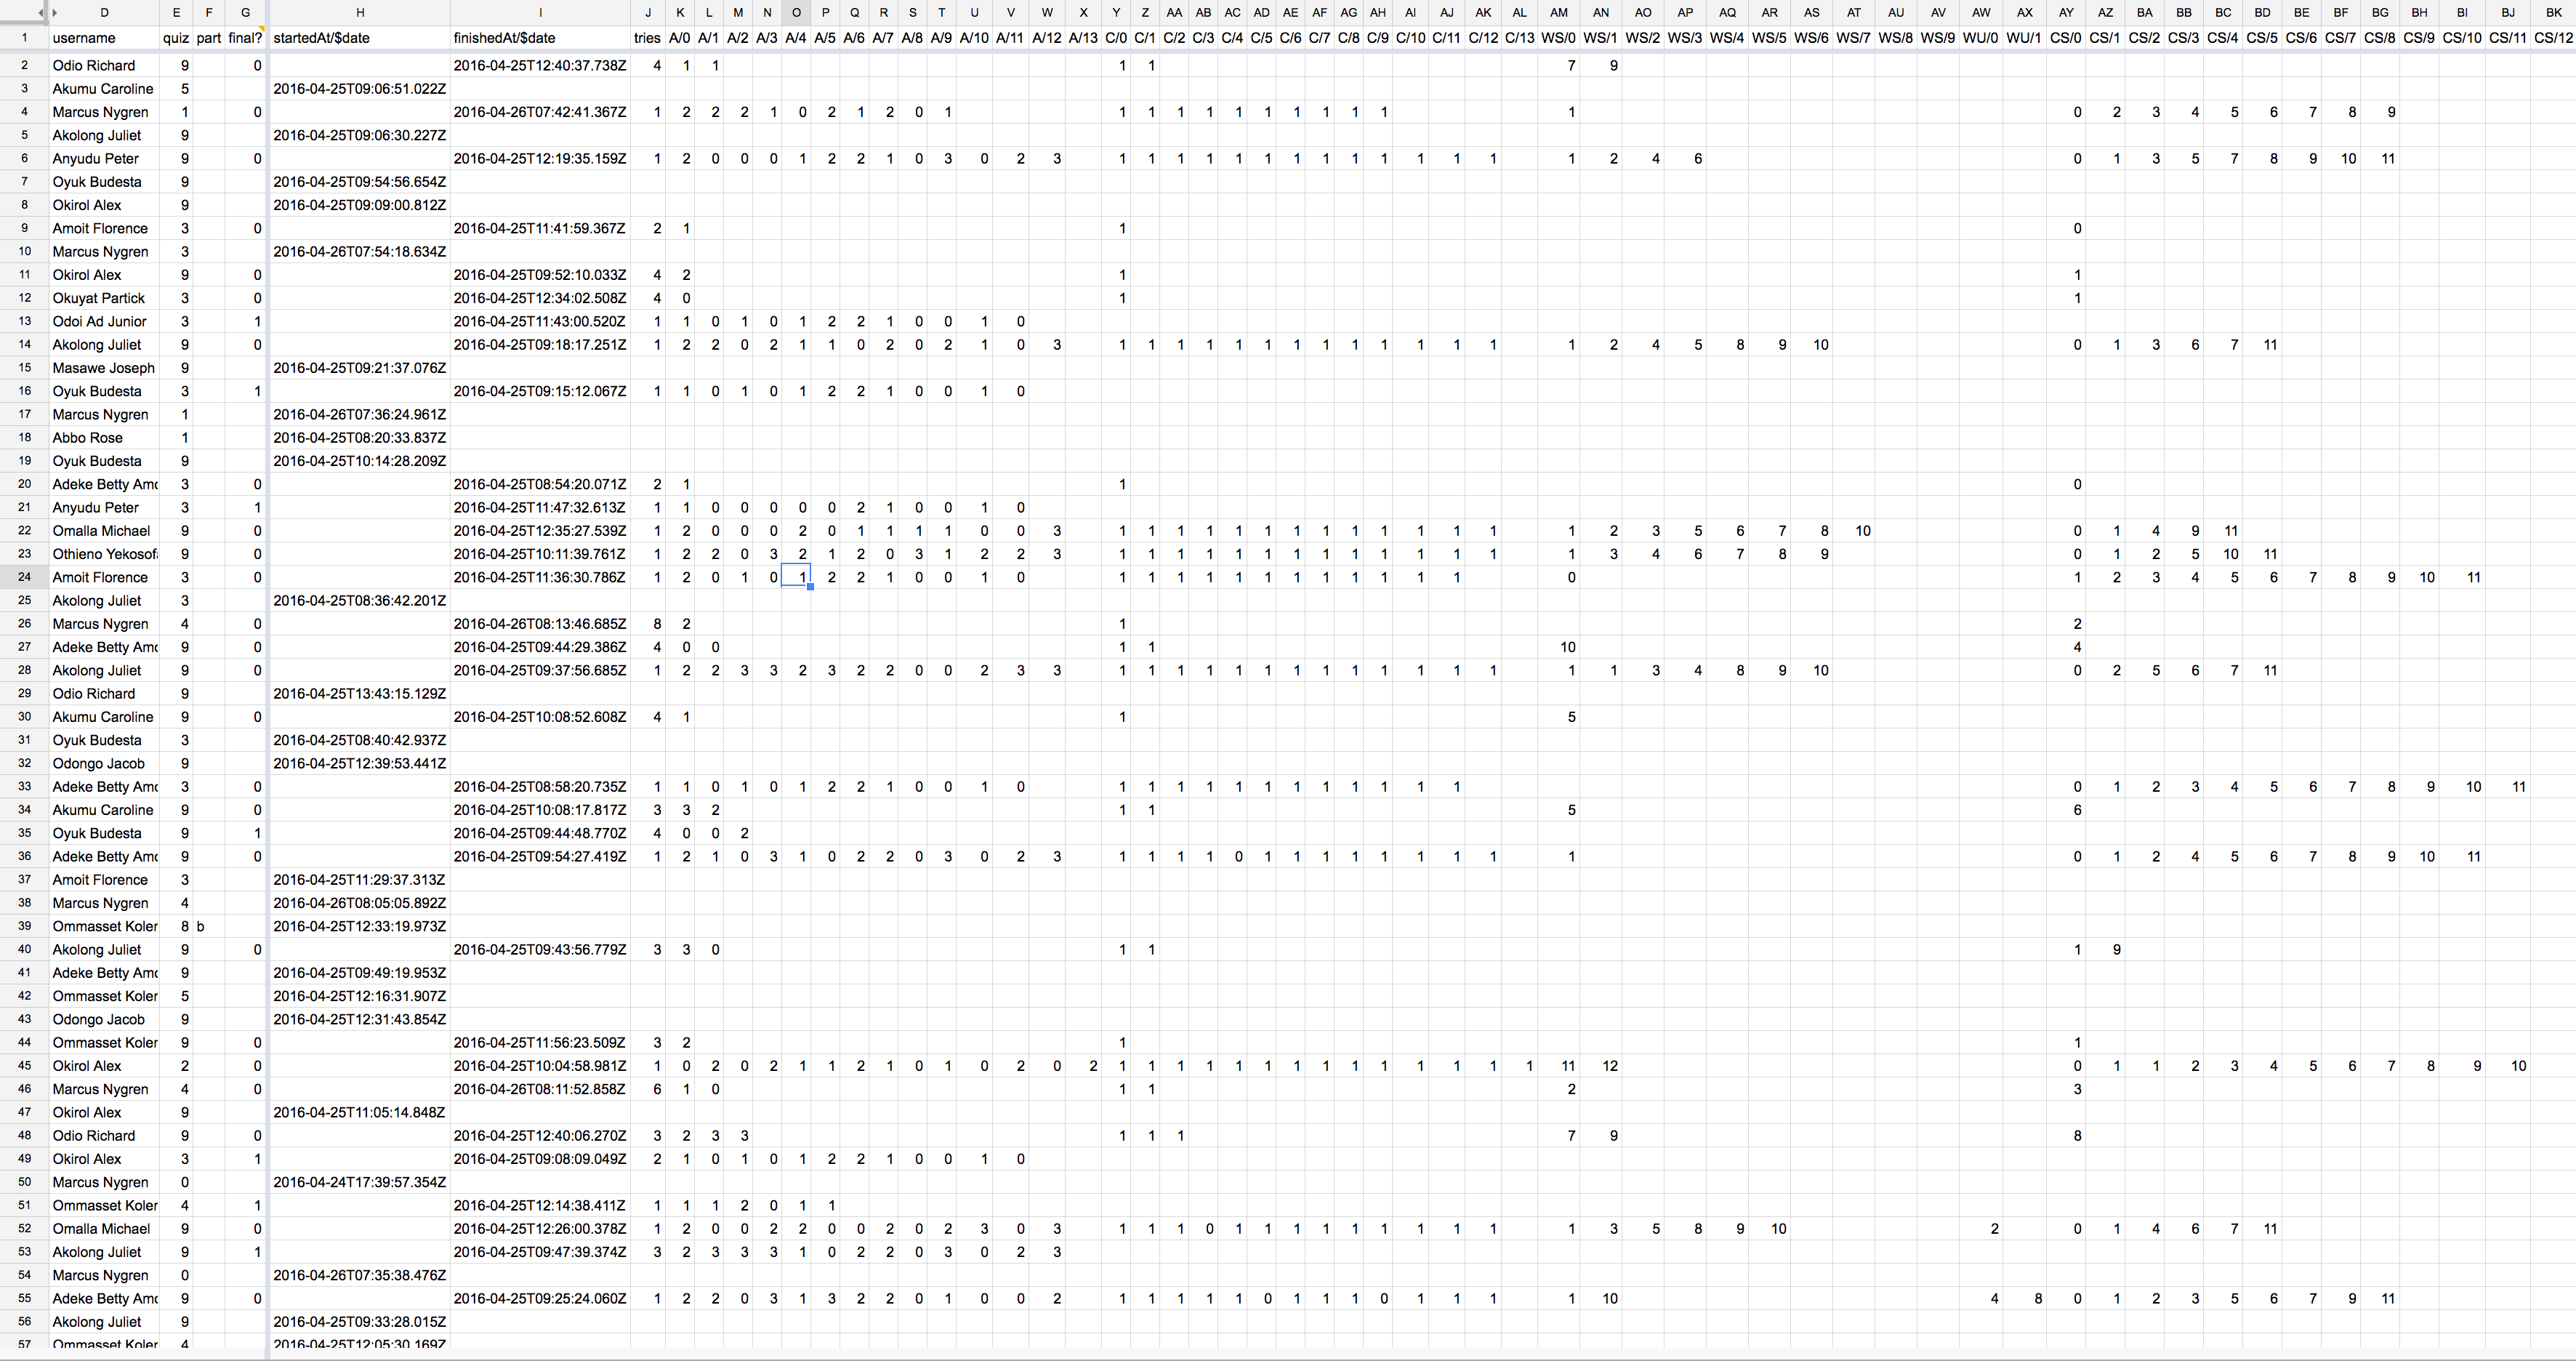
\includegraphics[width=0.8\textwidth]{analysis/unprocessedData.png}
  \caption{The raw data of the quiz results when inserted into Google Sheets.}
  \label{fig:unprocessedData}
\end{figure}

A lot of future development time should be spent so that most of this work is made automatically. Some of this work, is related to the way that the data is saved. Today, whether the coach was correct or incorrect on a question, and how many coaches answered that question incorrect after the first try, needs to be done by process of elimination, because the data is not properly structured in the database.

There were also a small number of errors with quiz submissions in iteration 4. Most notably, certification tests for coach quiz 9 were not submitted, which is why the paper submissions proved very valuable as a backup. To discover more errors regarding offline-online functionality, is important, as it is cumbersome and time-costly to test these manually. A good way to discover such errors, would be automatic tests (or regression tests), so that the app can be used by the coaches with confidence, without extra personnel present, checking that the app works.

\subsection{Code Quality}
Since the app will be continually used and developed by others in the future, code quality is important. React.js makes it easy to structure the code in a way that gives a new developer a good overview of the different components, and its functionality. Even so, refactoring the code into smaller components would be a good idea.

To increase speed of the app, refactoring the code to ensure that loading of assets happen more effectively (especially quiz questions), and also that data is cached in a logical way (saving neccessary information so that it does not need to load the same information again, and vice versa), would be helpful.

As the YoungDrive program grows and more people will use the app, there will be a lower tolerance for the app being slow. The app, especially on native, takes a long time to load, mosly because of asset loading.

\subsection{Internationalization}
During the Zambia tests, they were given a Zambia version of the app, and in Uganda, they were given a Uganda version.

In the future, it would be advisable if the coach ID used for login would affect if the Zambia version or the Uganda version should be shown.

Today it is acceptable that the app is solely in English, as it is understood by both the Zambia and Uganda coaches. As more countries are introduced, the app should be available in different languages.

A challenge today is that the Zambia uses a newer manual, and e.g. the national currency is different than Uganda's. That Zambia has updated manuals, means that some questions are new, some are removed, and some are re-formulated. But the teacher still wants to be able to compare quiz results between the different countries. Today, the quizzes were simply replaced between versions. This has the advantage of being easy to implement, but the clear disadvantage that the teacher can not compare quiz results between countries.

A good solution to internationalization of quizzes would be that each question in the database should include an unique ID, with different texts depending on country and coach manual. This would allow the teacher to keep track of some coaches have difficulties with a question, regardless of location.

\subsection{Availability on Old Android Devices}
Since the introduction of Meteor 1.3, older Android devices are no longer supported. For the YoungDrive coaches, this is an issue, as most often devices use older Android operating systems, and does not have great performance. Today, a Meteor 1.2 version of the app is available on the AppStore. Also, the newest version is avaialable on the web. However, in the future research should be put into if the app should abandon Meteor 1.3 altogether, or if there is another way to ensure backwards capability.

\subsection{Availability on Feature Phones}
As far from all coaches does not currently possess smartphones, few coaches will currently be able to use the developed app for preparing their youth sessions. Therefore, what was discovered in iteration 1, that all coaches possess feature phones, could guide the development of a SMS-based service. While this was not viable for the scope of the master thesis, research has been made into related work.

A recommendation is to try VOTO Mobile \cite{voto-mobile}, which supports multiple-choice questions and internationalization. Today, this solution has been used mostly for doing evaluations in rural areas, via automatic phone calls where the caller can be given responses in text. However, research on using such a solution for educational purposes seems promising.

\subsection{A bigger data sample would benefit answering the other research questions}
There are multiple examples how data analysis on a larger data sample could benefit answering the research questions. One such example is "Is the coach learning?". With enough data, it would be interesting to analyse the impact of feedback on getting the correct answer the next time. For example, you could compare if getting feedback on being wrong and unsure leads to better results than getting feedback on being wrong and unsure.


\subsection{Research question 2}
\section{How is the Design Affected by the Contextual Constraints?}

There were many things to consider when designing for the contextual constraints. Below, aspects that should be taken into consideration are presented.

\subsection{Replacing the Teacher}
In iteration 2, Josefina (the teacher) mentions that she does not want to be replaced by the app. However, there would be many benefits to YoungDrive if the coach training could happen 100\% digitally. When the app was tested with refugee innovators in iteration 2, several of them asked if it was possible for them to use the app exclusively to train themselves in entrepreneurship or starting a YoungDrive group.

How could it be done in practice? Also, when the teacher does not want to be replaced? In practice, a freemium model could be proposed, where it is possible to take the coach training for free digitally, but pay for a physical training. Currently, this contextual constraint has affected the app in the way that it should complement the physical training, and ease the burden for the teacher.

\subsection{Scaffolding the Coach Guides}
Josefina says after iteration 2 that it is indeed valuable if the training prepares the youth more actively for holding youth sessions, an insight that was discovered in iteration 1. She mentions two challenges with introducing coach guides for each topic. In the end, a solution is suggested:

\begin{itemize}
\item The coaches are not ready the first day, as they have not gotten used to the app yet. \textit{As such, they should be introduced in the middle of the training.}
\item A recurring issue is that the Friday, the last day of training, should be dedicated to preparing a session, but the time has never been there. If so, the coach guides will not be used. \textit{One idea could be to make the topic quizzes smaller, and mix topic questions with coach guide questions.}
\end{itemize}

\subsection{More Time Designing the App for Different Need Groups}
Already since iteration 1, different need groups have been identified. It is shown from the tests that the idealistic and realistic coach might be more probable to have a growth mindset, where challenged coaches might have a more fixed mindset. Continuing to use growth mindset feedback in the app is crucial according to \cite{dweck}, who found her method made lower and medium achievers also played until the end, while the lack of such feedback only kept high achievers.

Also, there are tendencies that different need groups are more present in different countries. While a lot of research was done about the cultural dimensions of Uganda, the research done on the Zambia and local Kabwe population was more sparse. It was known that the socio-economic differences were large, but not much more. For future work, it is recommended to put more work into how the local and national culture in a country affects the mentality of the coaches and the design. It is not possible to assume that the Zambia and Uganda culture should be similar, and it will be similar to other developing countries, or elsewhere.

Since doing app development together with the coaches has been so beneficial to discovering different needs, a wish is to have done more so with the coaches in Tororo. While in Zambia, the development was done in the real-world training, which was superb. In Uganda, more of the trigger material could have been created in Tororo instead of Kampala. Even if it would have been more costly and internet is slower, it would have been valuable being closer to the coaches.

\subsection{Training the Coaches with Using a Smartphone}
An additional insight from the smartphone test in iteration 1 was that using a smartphone operation system like iOS or Android needs to be made as easy as possible. This to avoid confusion with things like not finding the YoungDrive icon, or accidentally hitting a button, or click the power button: all of which relates to ease of using the operating system, and not to the app in itself. A lot of training is needed to avoid errors,  and should be taken into consideration from a service design standpoint.

In iteration 3, such a co-creation workshop was held after the app test. This resulted in that for iteration 4, all of the devices had the YoungDrive icon on the home screen of the device, and was the only noticeable app. This lowered confusion a lot with finding the app, and realising where to click. If a coach by accident clicked the home button, they immediately found their way back.

In the future, for new coaches, training how to use a smartphone is needed, before they are handed the device. While the YoungDrive is now simple to use to maybe not need an introduction, it would still help how to act in the app (for example encouraging to be honest with answering "Are you sure?").


\subsection{Research question 3}
\section{How can test questions be developed to support entrepreneurship learning?}

\subsection{Designing for honesty with "Are you sure?"}

\todo{Lägg till mer om att designa för empowerment}

One idea during the ideation of iteration 3, was to give the student two scores: one showing how correct they were, and one with how confident they were. You can be correct, but still not be empowered (you are unsure but correct). Similarly, you can be incorrect but confident (not empowered).

The reason for not having a "empowerment bar" (combining correct and sure, giving a summative score), was given by Josefina from YoungDrive: "The coaches might want to game the system to get a better score, or be confused by how they got their score". For this reason, the coaches have stated they accept getting minus points if the are sure but incorrect, which is easily understood by them and feels fair.

In the app now, there is still a struggle with coaches answering positive on "Are you sure?", even if they are not. Reasons are among others that they say they are \textit{partly} sure, and sometimes that they think they will be more punished for not being sure \textit{than} being sure and incorrect. As this is not the view of the teacher, this needs to become much more clear in the app. One idea is to ask "How sure are you?", but keep the binary scale of only two answers. This would mean, that the coach needs to think about \textit{how} sure she is about the answer, instead of \textit{if} she is sure, which could have metacognitive benefits.

\subsection{Self-reflection after a youth session}
When discussing the goals for iteration 3, Josefina talks about a need she has noticed during the coaches' rollout in Zambia, where the app could help: doing self-reflection after a youth session. She says that this is at least as important as the coach training, especially in cases where Josefina or other project leaders don't have the resources to visit the coaches physically.

It is determined that while physical follow-up meetings are essential, the app can be used to help the coach in a smart self-assessment and self-reflection. Also, on encounters with the teacher, it can guide the coach-teacher discussion.

This does not need to be a new app. Questions can be asked in a way that they are indeed meta-cognitive, encouraging learning by reflection.

Josefina mentions that when she is there to give feedback, it is very clear to the coach that he or she lacks knowledge and has not prepared enough.
%Asking: "What happens if you say X (giving the wrong information, e.g. what a cost is)?". "Why is it important that you answer correct on this question?".

An app with self-evaluation and monitoring, would help keep the coach thoughtful and give the coach important insights. They are described to sometimes over-estimate their own knowledge.

\subsection{Avoiding memorization}
To avoid memorization, the alternatives should be randomized in the future. While it is unlikely that a coach has an easier time remembering the correct answer by order instead of content, since they only repeats the wrong answers until the certification test, it is an extra measure.

\subsection{Improving the questions}
Data analysis of results on specific questions could give a lot of insight, both into coach behavior, and misunderstandings of questions, in the future. Here, a lot of data is already collected to be able to guide conclusions. Not only are questions recorded with correct and if answered confidently, but also number of tries per coach, and if it is a training quiz or certification quiz.

Simple analysis could be for example mean seeing what are the most difficult questions, where most people have answered wrong repeatadly. From the interviews in iteration 4, it is explained that some answers might be answered wrong becuase of for example difficult wording of questions, not neccesarily because of lack of knowledge. To avoid this, data analysis could be effective, together with getting input from the teacher and coaches.

Improving the questions today has mostly been made from direct feedback from the coaches, or comparing quiz question formulation with current and desired level on Bloom's revised taxonomy. Regarding mapping educational objectives, it needs to be made sure that there are questions for each educational objective of the topic, which has not been done today. In \cite{yengin} questions were designed to support gradual knowledge building with an alignment to Bloom’s Taxonomy, which could also be a viable alternative for this app, where questions are currently formulated as information appears in the participant and coach manual respectively.


\subsection{Research question 4}
\section{How does Design Affect Usability and Learning Done via the App?}\label{sec:future-work-4}

There is a clear connection between design and usability and learning. Here, future work for how design would improve usability or learning is presented.

\subsection{Assessing Coach Guide Knowledge Before the Youth Session}
When asked about the Zambia coach rollout, Josefina points out several challenges. "It feels like some of the coaches forget using the coach guide, even if it has been improved and better integrated with the participant manual. Some of them, don't even use the coach guide." This speaks for that the app should include quizzes for all coach guides as well. When asked if the coach guide quiz are more important than the topic quizzes, she answers that the correct knowledge is more important, because that is the one that needs to be explained correctly to the youth. Therefore, it should be moved into Future work.

\subsection{Using a Flashcards Approach}
In the ideation for iteration 2, flashcards are discussed again, with Henrik Marklund. In iteration 3, this was tested as a lo-fi material with successful results, but more work should be done.

In the ideation of iteration 4, a proposal was given that did not have time to implement. Therefore, the idea is described here: At the coach's second quiz try (having assessed and reflected on the knowledge), flashcards could be introduced to assist the coach in retrieving from memory, before getting the multiple-choice. For future work, when in Training after the first quiz try, The question should be shown \textit{before} the answers are shown, and prompt the coach to think aloud about what they think the answer is, before receiving the alternatives. The coach might be hindered from progressing to the multiple-choice answers until the app has understood the coach has thought hard about their answer to the question.

This is a good use of scaffolding, slowly introducing complicated app features. The hypothesis is inspired from \cite{bjork}, that knowledge is strengthened if the coach retrieves from memory, versus looking up the answer or choosing the most likely answer.

\subsection{Adding more media channels to more closely simulate the learning environment}
To simulate the entrepreneur coach environment more accurately could possibly increase memorization of procedural learning objectives. Research exists that supports how using multiple channels like audio, video, voice could be beneficial, or to use interactive simulations.  The advantage of multiple-choice from a developer perspective is that data can be collected easily and because of ease of implementation. From YoungDrive's perspective, it serves the target group of the coaches being first-time smartphone users well \citep{youngdrive-masterthesis-idea}.

\subsection{Improvements to the Certification Mode}

Following the advice from \cite{sierra} of quickly giving the user a feeling of a superpower, this should be becoming a Certified coach in the future. From the end results of iteration 4, we can learn that notably the intrinsic motivation is high, deliberate practice is present, and the coach can feel the intrinsic reward of having pushed herself and learned the material when certified. This is very positive.

This reaction, could and should be even more amplified when certified. It is discussable if this should be done by simple gamification, but an opinion by a coach was that medals earned should be more visible and that sounds could strengthen the feeling of achievement. Also, the quiz list could show these results, increasing motivation to take other quizzes that you have not yet mastered, or to better your score in a topic where you had not become certified.

\subsection{Improvements training Correct Structure and Time Management}
During all app tests (iteration 2-4), it has been shown that since Correct Structure and Time Management are both ordinal, the Training mode for such topics would be more suitable as interactive exercises than multiple-choice. The proposal is to first use drag-and-drop to place each activity of a youth session in the correct order, and then selecting the right time for the each activity. This assists the coach in creating a mental model, which can be used to retrieve from memory during the assessment.

\subsection{Scaffolding with Flashcards}
After the coach's first new try, Flashcards could be introduced to assist the coach in retrieving in memory, before getting the multiple-choice. To do this after the first assessment, is partly because of technology scaffolding (introduce new concepts in steps), partly because the knowledge is strengthened if the coach retrieves from memory versus looking up the answer or choosing the most likely answer \citep{bjork}.

\subsection{Memory Design}
For the ideation of iteration 4, it was pointed out by pedagogical expert Henrik Marklund that if knowledge is to be memorized, memory techniques could be used. One such e-learning tool is \cite{memorize}. The tool has interactive learning modes, aiming to learn facts and terms with speed. This was not prioritized because of time constraints working with technical features that were not essential. Also, the idea was never proposed by users, only by experts. Moreover, the teacher opposed the idea of remembering answers that were not in the factual remember category. To do so, would oppose the learning objectives, which score higher on Bloom's revised taxonomy. However, to study how the coaches can remember better via an app, and learn memory techniques via the app, could be a future work which is advisable.

\subsection{Sharing with One Another}

In future versions of the app, mechanics of sharing content and co-creation would add value connected to Bloom's, reaching Create and Apply. Adding these game elements goes in line with Clark's research, which showed a positive correlation with learning and games that required multi-player collaboration \citep{gates}.


\subsection{Including the Paper Manuals in the App}

Already in iteration 2, it was proposed by coaches if the participant manual and coach guide could be included in the app, instead of as paper. The teacher agreed in principle, especially as the paper coach guide is often overlooked (reading the digital version could be designed to be made mandatory before unlocking other features), but also saw several challenges.  Because of broadband limitations the manuals would take a lot of space to download. Also, the manuals are designed in A4 format, while a smartphone screen or even tablet is much smaller, making it cumbersome to read the whole manuals in the same way you would with the paper versions.

However, for the ideation of iteration 3, it was realized that if the manuals could be converted into smaller chunks, there is an opportunity for bite-sized spaced learning, instead of massed learning. How to split the manuals into these small parts? Well, by extracting the important parts for understanding an answer to a specific question, see figure \ref{fig:bite-size}. The teacher emphasised that this would take time for her to do, but that the effort would be worth it. While there was no time for including the whole manuals, there was an idea the teacher thought acceptable for iteration 4: including on which page the coach would find the answer to a specific question. This was not one of the most prioritized features of iteration 4, which it was never done, but for further work, this should be investigated.

\begin{figure}[h]
    \centering
    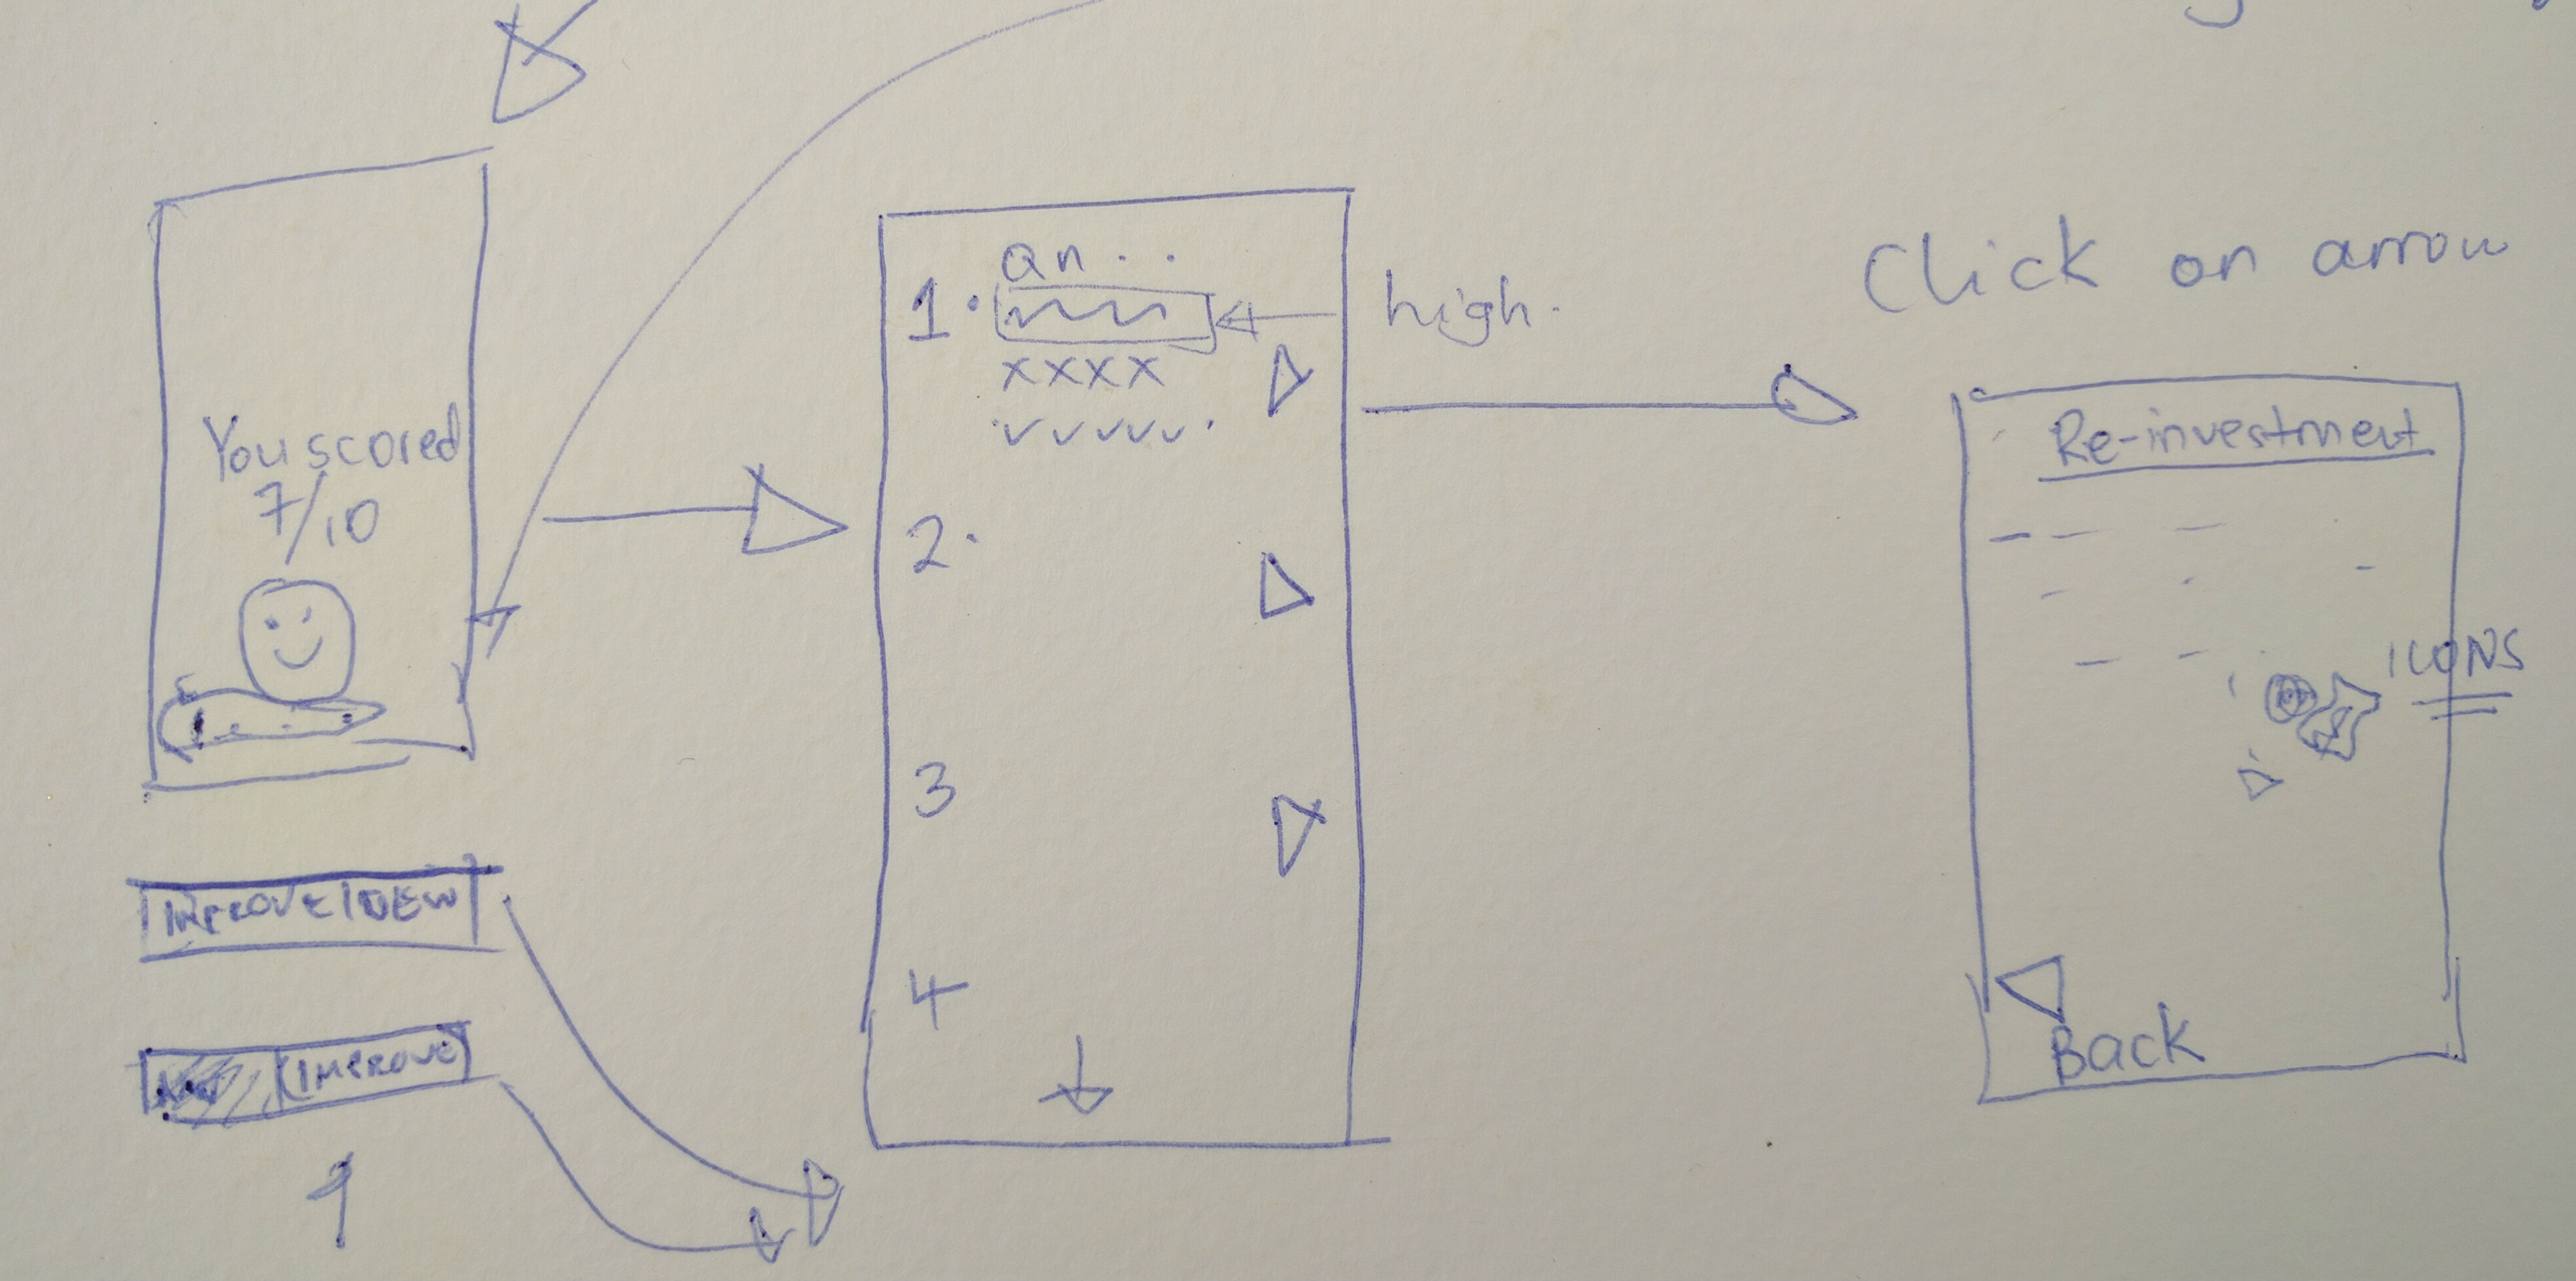
\includegraphics[width=0.8\textwidth]{biteSize.jpg}
    %IterationProcess.png
    \caption{By clicking on an arrow next to the question showing the correct answer compared to your answer, the coach could read an extract from the YoungDrive manuals, which includes the right answer. The learning benefit compared to just observing the right answer, is that the coach gets the answer in context, which improves memorization and understanding. An idea would be to no longer give the coach the correct answer in the score board, but to instead let the coach choose the right answer after reading the text.}
    \label{fig:bite-size}
\end{figure}

A major opportunity doing this would be to replace the paper manuals. Today, the manuals are the most expensive post of YoungDrive, which is why this would be attractive. While a smartphone or tablet could be returned after a YoungDrive program has ended, this is not possible with the paper versions, so there might be a monetary incentive to do so. A problem that would need to be addressed is that the manuals also have written exercises in them. These exercises could be made interactive in the app, which would also allow for smart features such as automatic assessment, financial literacy simulations, etcetera. While this was not a scope of the master thesis, it is interesting further work to test if such interactive exercises and simulations would be effective in the developing country context of learning and teaching entrepreneurship.


\subsection{Research question 5}
\subsubsection{\#5 Educator Dashboard}
Josefina has no means of accessing live quiz results today, as there is no educator dashboard developed. Instead, quiz results today needs to be transferred from a database into Google Sheets, which is cumbersome and not user-friendly.

There was not enought time to develop an educator dashboard, even if this had been a goal. Instead, low-fi trigger material was created, and co-creation stakeholder workshops were held, both for iteration 3 and 4.

In the future, this will be a must-have, and it ties well into YoungDrive's future wish of strengthening its quality assurance via monitoring and evaluation.

How powerful the educator dashboard should be might be a ethical discussion, where one could argue that me as a developer needs to be sensitive if I want the app to support the coaches to become better, and not be a tool for the project partner to fire coaches that doesn't have the same quiz results as others. As the combination of "Are you sure?" and correctness can give insight into the attitudes and care of the coaches, carefulness must be taken.

 %då Expedition Mondial ifrågasatte "Visst är väl även Christine och Patrick?" målgrupp för detta? Och vad har de för utrustning? Christine har mobil, Patrick ingen. Så detta talade för att Educator Dashboard skulle behöva fungera på mobil, och inte bara dator som jag tänkt, iom att Josefina har dator.

%Då bestämdes med Expedition Mondial att jag skulle ha workshop med dem på onsdag. Med samtal med Josefina, sade hon att de garanterat borde utrustas med tablets då de samlar in data digitalt, så jag kan tänka mig att de får en tablet framöver. Skönt! Detta stämmer även med vad Stefan FalkBoman hade tänkt sig, och de iPads han köpt in till mig. Så då kunde jag ha dessa som tanke att utforma educator-app-dashboarden ifrån.




%\chapter{\rtthesis documentation and \LaTeX{} tips}\label{cha:rtthesis}

This document is not only an example that you can use to get started with the \rtthesis class, it also contains written instructions for how to use the class, and some general tips on how to use \LaTeX{} to produce a beautiful thesis.  As we do so in this chapter, we also get the opportunity to look at some theorem-like environments, which you can alter the look of by changing the options given to the \rtthesis class.

\section{Basic setup}\label{sec:basic-setup}
%
You must decide on an input encoding from start, and select the corresponding class option from \tableref{tab:inputenc} on \pagepageref{tab:inputenc}.  You must also tell \rtthesis whether you intend to use part sectioning or not, see \tableref{tab:part-options}.  There are many more class options, but they will be mentioned below where there is room for a more detailed discussion for the corresponding features.

Information about the thesis, which is needed to produce the thesis itself as well as the thesis cover and the “spikblad”, is passed to \rtthesis using the command \texcommand{setupThesis}.  The command is called in the following way, where the most common key-value pairs are listed in \tableref{tab:setupThesis} (the remaining key-value pairs concern master's theses, see \sectionref{sec:msc})):

\begin{minipage}{1.0\linewidth}
  \verbatimsize
\begin{verbatim}
\setupThesis{
  key1=value1,
  key2=value2,
  ...
}
\end{verbatim}
\end{minipage}

If a PhD thesis has an interesting illustration on the cover, it is customary to provide a caption for the illustration.  The caption will be printed on the back of the title page, and is set up by redefining the command \texcommand{rtcoverinfo}.  For instance, it may look like this:

\begin{minipage}{1.0\linewidth}
  \verbatimsize
\begin{verbatim}
\renewcommand{\rtcoverinfo}{\textbf{Cover illustration:}  Block
diagram showing the structure of the control scheme proposed in
\chapterref{cha:cool-control}}
\end{verbatim}
\end{minipage}


\begin{table}[tbp]
  \centering
  \caption{\label{tab:part-options}%
    Class options that inform \rtthesis whether part sectioning will be used or not.}

  \begin{tabular}{l p{0.5\linewidth}}
    \toprule%
    \textbf{Class option} & \textbf{Meaning} \\
    \otoprule%
    \classoption{parts} & Prepare for \texcommand{part} as the topmost sectioning command.\\
    \classoption{noparts} & Prepare for \texcommand{chapter} as the topmost sectioning command.\\
    \bottomrule%
  \end{tabular}
\end{table}

\begin{table}[tbp]
  \centering
  \caption{\label{tab:setupThesis}%
    Key-value pairs recognized by \texcommand{setupThesis}.  Note that values that include white space are surrounded by braces.}

  \begin{tabular}{>{\ttfamily}r !{\texttt{=}} >{\ttfamily}l p{0.5\linewidth}}
    \toprule%
    \textbf{Key} & \textbf{Example value} & \textbf{Comment} \\
    \otoprule%
    author & \{My Name\} & \\
    title & \{Thesis title\} & \\
    subtitle & \{Good stuff\} & Optional. \\
    city & Norrköping & Default: \emph{Linköping} \\
    year & 2010 & \\
    isbn & isbn-isbn-isbn-isbn & \\
    type & phd & Must be either \emph{phd}, \emph{lic}, or \emph{msc}. \\
    thesisNo & 9999 & Number in series (the series is determined by the choice of thesis type). \\
    localID & 11 & Only used for licentiate's theses.  It is the last part of the local identifier \emph{\mbox{LIU-TEK-LIC-2010:11}} in this case.\\
    username & isyusername & Used to generate the author's email address. \\
    dedication & \{To my parents!\} & \\
    \bottomrule%
  \end{tabular}
\end{table}

\section{Page layout and related options}\label{sec:page-layout}
%
Theses are restricted to the S5 paper size.  How the S5 page is organized is up to you, but \rtthesis only allows you to choose from two predefined layouts, and only one of them is recommended.  To get your own layout you should make a copy of \textfilename{rtthesis.cls} and modify the code for one of the existing class options for layout.  The class options for page layout are given in \tableref{tab:page-layout}.

At the time of writing, the printers used by LiU-Tryck print on A4 paper (physical size), which is then cropped to S5 (logical size).  Similarly, when you print draft versions of your thesis on your office printer, it is very likely that the used physical paper size will be A4.  Hence, it makes sense to let \rtthesis control how the S5 logical page is placed on the A4 physical paper.  In this case, \rtthesis will produce a \textsc{pdf} with pages in the A4 format, with content restricted to the S5 format.  On the other hand, when you produce a \textsc{pdf} that is meant to be read on a computer screen, the page size should be exactly S5.  When targeting the A4 physical format, it is possible to get crop marks for the S5 box, and to put some information about each page outside the S5 box.  The related class options are given in \tableref{tab:page-layout}.

To ensure that you really get the page layout you think when you send your thesis file to the printer's, the best option \emph{should} be to use the \classoption{crop} option.  However, they will tell you differently, since they think it's \emph{their} job to position the logical page on A4 and add crop marks.  Unfortunately, there is a lot of manual work in the process, so there is a (substantial?!) risk that the content of your pages will be shifted with respect to the S5 box of your layout\ldots

\begin{table}[tbp]
  \centering
  \caption{\label{tab:page-layout}%
    Class options related to page layout.  The most important one to remember is \classoption{crop} (since  \classoption{S5} and \classoption{pdf} are default).}

  \begin{tabular}{l p{0.5\linewidth}}
    \toprule%
    \textbf{Class option} & \textbf{Meaning} \\
    \otoprule%
    \classoption{S5} & Recommended layout.  Margin paragraphs are tiny (see \sectionref{sec:research:history} for examples), and should only be used for comments that will be removed in the final version of the thesis.  Default.\\
    \classoption{S5MP} & Layout to use if you are serious about margin paragraphs.  Not recommended, since the S5 format is too narrow to really fit margin paragraphs of reasonable width. \\
    \classoption{nailing} & Layout for the “spikblad”.  Not for theses! \\
    \midrule%
    \classoption{pdf} & Produce pages in the S5 format.  Default.\\
    \classoption{onA4} & Logical S5 page on a \textsc{pdf} page of size A4.\\
    \classoption{info} & Write information about each page above the logical S5 page.\\
    \classoption{crop} & Same as \classoption{onA4} with \classoption{info} and crop marks.\\
    \classoption{noInfo} & Turn off the effect of \classoption{info}.\\
    \classoption{draft} & Same as \classoption{onA4}, but pictures are blank and overfull \texttt{hbox}es stand out.\\
    \bottomrule%
  \end{tabular}
\end{table}

Although only weakly related to page layout, this section ends with a tip for how to change the size of the chapter numbers (some users find them much too big).  The font is controlled using the \styname{sectsty} package, and it follows that it can be redefined by, for instance,

\begin{minipage}{1.0\linewidth}
  \verbatimsize
\begin{verbatim}
\chapternumberfont{\fontsize{60mm}{63mm}\selectfont}
\end{verbatim}
\end{minipage}

\section{Front-matter environments}

There are environments defined for typical sections in the front-matter\footnote{The \emph{front-matter} is everything that goes in the beginning of the thesis, before the page numbered~\emph{1}.}.  The most important purpose of providing these environments is that they take care of the table of contents and the \textsc{pdf} bookmarks for you.  The environments are \envname{abstract}, \envname{preface}, \envname{acknowledgments}, and \envname{notation}.

The environment \envname{abstract} accepts the language used inside the environment as an optional argument (which defaults to \texttt{english}).  If the language is set to \texttt{swedish}, the title of the abstract will be \emph{Populärvetenskaplig sammanfattning}, in accordance with the Linköping University requirements on theses written in English.

Inside the \envname{notation} environment, you can put anything you like, and maybe the \envname{notationtabular} environment provided by \rtthesis suits your needs.  In order to define this environment, \rtthesis loads the two packages \styname{array} and \styname{ctable}, and also defines the command \texcommand{otoprule} to mean the same as \texcommand{toprule}.  See \tableref{tab:notationtabular} regarding how to change the look of \envname{notationtabular}.

\begin{table}[tbp]
  \centering
  \caption{\label{tab:notationtabular}%
    Legal option values to the \envname{notation} environment.  The options control the look of the \envname{notationtabular} environments used inside the \envname{notation} environment.  The initial definition of \envname{notationtabular} is the same as that obtained by passing the option \classoption{new}.}

  \begin{tabular}{l p{0.5\linewidth}}
    \toprule%
    \textbf{Option} & \textbf{Meaning} \\
    \otoprule%
    \emph{emty} & Do not redefine \envname{notationtabular}.  Default.\\
    \classoption{old} & Make \envname{notationtabular} produce a plain \LaTeX{} table with double horizontal lines under the table headings, and a vertical line separating the two columns.\\
    \classoption{new} & Make \envname{notationtabular} produce a table according to the guidelines in \citet{Mori07Tables} using the \styname{ctable} package.\\
    \bottomrule%
  \end{tabular}
\end{table}

There is a class option called \classoption{noextras}, which was intended to inhibit the effect of the \texcommand{maketitle} command, and redefine the front-matter environments to not produce any output.  However, the option is not working well at the moment.  On the other hand, as the time it takes to compile a thesis on a modern computer is very short, it is rather unclear why someone would like to use this feature anyway.


\section{Abbreviations}

Automatic control is a \LaTeX{}-friendly community.  This means that everything you produce is expected to look good.  We begin with a basic result.

\begin{theorem}\label{th:abbr-in-sc}
  Abbreviations, such as \abbrARMA, look best in small caps.

  \begin{proof}
    Just compare with “ARMA”.
  \end{proof}
\end{theorem}

However, it is important that the small caps match the sorrounding text, compare the statement in the theorem above with the following variation of it, in italics instead of slanted text:
\begin{quotation}
  \noindent\textit{Abbreviations, such as \abbrARMA\footnote{This will cause a \LaTeX{} warning.} or {\normalfont\textsc{arma}}, will stick out in a terrible way if you don't watch out!}
\end{quotation}
This is why the \rtthesis class uses slanted text rather than italics in theorems rather when slanted small caps are available.

Unfortunately, \rtthesis does currently not provide a way to make small caps look good in italics, which leads to the following corollary to \theoremref{th:abbr-in-sc}.

\begin{corollary}
  One has to make a choice between
  \begin{itemize}
  \item Beautiful abbreviations using small caps (instead of ordinary upper case).
  \item Pretty text typeset in italics (instead of slanted text).
  \end{itemize}
\end{corollary}

\section{Definitions}

Let us discuss another theorem-like environment while we have some examples of similar environments to compare with in the previous section.  That is, let us discuss the \envname{definition} environment (and the similar environments \envname{assumption} and \envname{remark}).  All the theorem-like environments are defined in a separate package, \styname{rtthesis-theorems}, so that they can be used with other document classes as well.  The definition below is an example of a definition with a title.

\begin{definition}[Definition]
  A \emph{definition} is a precise explanation of the meaning of a word or concept.  It may be tempting to include examples in a definition, but a good definition should not depend on examples as part of the definition.  However, examples are often useful to clarify a definition, and should appear near the definition.

  A short definition may require just a single paragraph, while a more complex definition may require a few paragraphs.  Some definitions will also make use of displayed math.
\end{definition}

One problem one has to consider if definitions are not restricted to just one paragraph, is how to show the reader where the definition ends.  In theorems, it is common to use italics or slanted text (for brevity, we will not mention italics from here on) to show where the theorem statement ends, but for definitions it may be desirable to use the slanted text to emphasize the word or concept being defined.  (It is arguably more clear to highlight the new word or concept using slanted text with upright surrounding text, than vice versa.)  To use an upright font for the definitions may also be a way of avoiding to heavy use of slanted text.

Various options related to the appearance of theorem-like things (in \LaTeX{}, a definition is a kind of theorem) are described in \tableref{tab:theorems}.  \Tableref{tab:definitions} (used also to illustrate tables) contains some suggestions regarding combinations of options for the \envname{definition} environment and options for paragraph breaks.

\begin{table}[tbp]
  \centering
  \caption{\label{tab:theorems}%
    Class options related appearance of theorem-like environments.  The \emph{theorem-like environments} defined by \rtthesis are \envname{theorem}, \envname{proposition}, \envname{lemma}, \envname{corollary}, \envname{definition}, \envname{assumption}, and \envname{remark}.  The \emph{definition-like environments} are a subset of the \emph{theorem-like environments}, consisting of the environments \envname{definition}, \envname{assumption}, and \envname{remark}. See also \tableref{tab:fonts} regarding the fonts used in theorems.}

  \begin{tabular}{l p{0.5\linewidth}}
    \toprule%
    \textbf{Class option} & \textbf{Meaning} \\
    \otoprule%
    \classoption{break} & Put line breaks after the titles of the environments \envname{theorem}, \envname{proposition}, \envname{lemma}, and \envname{corollary}.\\
    \classoption{nobreak} & Never put line breaks after titles of theorem-like environments.  Default.\\
    \midrule%
    \classoption{definition=naked} & Definition-like environments look like the surrounding text, and are only isolated by some vertical white space.  Default.\\
    \classoption{definition=theorem} & Definition-like environments use same font as the \envname{theorem} environment, and are isolated by some vertical white space.\\
    \classoption{definition=marks} & Definition-like environments look like the surrounding text, and are isolated by small marks.  Strongly recommended if \classoption{parskip} is used.\\
    \midrule%
    \classoption{nosharecounter} & Use separate numbering sequences for each theorem-like environment and the \envname{example} environment.\\
    \classoption{sharecounter} & Use one numbering sequence for theorem-like environments, and the \envname{example} environment.\\
    \bottomrule%
  \end{tabular}
\end{table}

Sometimes, a definition may be given without a title.  The next definition is an example of this, even though it is questionable whether it was a good idea to omit the title in this particular case.

\begin{definition}
  An \emph{environment} in \LaTeX{} is a construct that is entered with the command \texcommand{begin\{\ldots\}} and exited with the command \texcommand{end\{\ldots\}}, where “\ldots” should be the name of the environment.
\end{definition}

In \tableref{tab:theorems}, there are three options related particularly to how \envname{definition}, \envname{assumption}, and \envname{remark} are typeset.
\begin{itemize}
\item With \classoption{definition=naked} (default) the definitions are typeset in upright font, and there is nothing on the page that marks the end of the definition.
\item With \classoption{definition=theorem} the definitions are typeset in the same style as theorems.  Since theorems are supposed to be typeset in slanted text, this will make it clear where the definition ends.
\item With \classoption{definition=marks} the beginning and end of definitions will be indicated with small marks.  Compare how the end of a proof is marked with a square box!  The current implementation has some problems with placing the marks if the definition ends with a displayed equation, but this can be compensated for by manual insertion of a \texcommand{vspace} command.
\end{itemize}

You may judge from the following example whether manual insertion of a \texcommand{vspace} command is necessary to make the definition ending with a displayed equation look alright.

\begin{definition}
  The factorial (denoted by the postfix operator $!$), defined for natural numbers, is given by
  \begin{equation*}
    n! =
    \begin{cases}
      1, & \text{if $n = 0$} \\
      n \cdot (n-1) \cdot \dotsc \cdot 1, & \text{otherwise}
    \end{cases}
  \end{equation*}
\end{definition}

This paragraph only serves to highlight the vertical white space below the definition ending with a displayed equation.  Note that one way to avoid problems with this kind of definitions is to rewrite them so that they don't end with displayed equations.

All definitions in this section have been entered as isolated paragraphs; that is, there is an empty line in the source code of the document before and after each \envname{definition} environment.  Although not recommended, \rtthesis supports definitions that are connected with the preceding paragraph, in which case the usual vertical space (if any) between paragraphs will not be inserted.  \emph{Be careful so that you don't omit the paragraph breaks by mistakes, since it makes a difference that may be hard for proofreaders to spot!}  As an example of a definition written in the same paragraph as the preceding text,
\begin{definition}
  A \emph{paragraph} (according to Oxford American Dictionaries) is a distinct section of a piece of writing, usually dealing with a single theme and indicated by a new line, indentation, or numbering.
\end{definition}
There is no paragraph break in the source code between the definition above and this text, but currently this cannot be seen in the typeset document.  If you know how to solve this, let the \rtthesis maintainer know!  If you want to learn about the \TeX{} mechanisms involved, see \citet{RyckoJackowski93TeXIndentPar}.

\section{Theorem titles}
%
The class lets you control the white space that separates a theorem title from the theorem statement.  The options appear in \tableref{tab:theorems}.  With the class option \classoption{break} (default), you will get a line break.  With \classoption{nobreak}, you will just get horizontal space.  Not all types of theorem-like environments will be affected by the \classoption{break} option, so to get things exactly they way you want, you may have to make your own modified copy of the \rtthesis class.  Try to recompile the document with the two different options and compare the result!

\section{To share or not to share counters}\label{sec:rtthesis:sharecounter}
%
Other things to think about regarding style include whether to use the same counter for all sorts of theorem-like things.  Again, the options appear in \tableref{tab:theorems}.  Some like to make the number of important theorems to stand out by having a separate counter (as in \citet{Khalil02NonlinearSystemsBook}), while other prefer to use as few counters as possible in order to make it easy to locate referenced items (as in \citet{Rugh96LinearSystemsBook}).  The two alternatives are supported in \rtthesis, via the options \classoption{sharecounter} and \classoption{nosharecounter}.

\section{Completely customized theorem-like environments}\label{sec:rtthesis:custom-theorems}
%
If you don't like the way \rtthesis sets up theorem-like environments (listed in the caption of \tableref{tab:theorems}) for you, you may pass the class option \classoption{notheorems}.  Then \styname{amsthm} will not be loaded, none of the theorem-like environments will be defined, and it is up to you to define your own environments.  If you decide to do so, using the \styname{amsthm} package will be a good idea.

\section{The \envname{example} environment}
%
The \envname{example} environment defined by the \rtthesis class is \emph{not} a floating environment, but is simply used to highlight that the text inside the environment is just an example of something more general that you have explained before.  Just as with the theorem-like environments, the environment is defined in a separate package, \styname{rtthesis-example}, so that it can be used with other document classes as well.

\begin{example}
  As an example of the \envname{example} environment, we include a little example here.  You can use this example to see how the options described in \sectionref{sec:rtthesis:sharecounter} affects the numbering of the environment.

  Depending on where this example ends up in the typeset document, you may also have the chance to see the ugly stretched vertical space that sometimes appears at the top and bottom of the environment.
\end{example}

There are three lengths you may play with the fine tune the appearance of examples, explained in \tableref{tab:example-lengths}.  Clearly, it would be possible to introduce additional parameters, but currently the corresponding aspects of the environment are hard-coded into \rtthesis.

\begin{table}[tb]
  \centering
  \caption{\label{tab:example-lengths}%
  The lengths used to control the appearance of the \envname{example} environment.  Note that the environment tries to compensate for the current value of \texcommand{parskip}, so you may not always get exactly what you'd expect.  Also, the meaning of the distance between the upper stroke and the text is somewhat arbitrary in order to allocate space for the example title.}

  \begin{tabular}{>{\small\ttfamily}l p{0.1\textwidth} p{0.4\textwidth}}
    \toprule
    {\normalsize\normalfont\textbf{Length}} & \textbf{Default} & \textbf{Purpose} \\
    \otoprule
    $\backslash$exampleLineWidth & $\unit{0.6}{pt}$ & Thickness of the strokes. \\
    \midrule
    $\backslash$exampleTopBotInnerMargin & $\unit{2}{ex}$ & Vertical space between strokes and contents of the example. \\
    \midrule
    $\backslash$exampleTopBotOuterMargin & $\unit{1}{em}$ \texttt{plus} $\unit{1}{ex}$ \texttt{minus} $\unit{1}{ex}$ & Vertical space surrounding the example. \\
    \bottomrule
  \end{tabular}
\end{table}

As is mentioned in the example above, there is sometimes problem with vertical space at the top and bottom of the \envname{example} environment.  During the page breaking process (see \sectionref{sec:tipt:page-breaking}) you could consider to add something like
{\verbatimsize
\begin{verbatim}
  \vspace{-1\baselineskip}
\end{verbatim}}
to reduce such artifacts.  Even better, if you know how to correct this in the definition of the environment, let the \rtthesis maintainer know!  The paper \citet{RyckoJackowski93TeXIndentPar} is recommended for anyone interested in the lesser known details of \TeX{} that one has to grasp in order to really solve the problem.

\section{Captions}\label{sec:rtthesis:captions}
%
The \rtthesis class loads the \styname{captions} package to obtain good-looking captions.  Captions are set up assuming that table captions will be placed above the table they belong to.  Many authors find this confusing since figure captions are always placed below the figure they belong to.  If you want to put table captions below the table you need to adjust the spacing around the caption by putting the following line in your personal style file:
{\verbatimsize
\begin{verbatim}
\captionsetup[table]{position=bottom}
\end{verbatim}}

Note that the command above only changes the spacing around the caption.  You still have to put the code for each caption relative to the tabular itself consistently with the captions setup.  Two tables are included in this document for illustration.  \Tableref{tab:definitions} indicates the many combinations of options that the \envname{definition} environment has been designed to work with.  The next one, \tableref{tab:chapters} is just a stupid table telling where the different chapters in this document begin.  For comparison, a typical automatic control block diagram has been included in \figureref{fig:feedback}.

Some nice guidelines for table creation in \LaTeX{} are given in \citet{Mori07Tables} (it is just two clicks away!).

\begin{table}[p]
  \centering
  \caption{\label{tab:chapters}%
    Different combinations of class options that affects the \envname{definition} environment.  The code for this caption appears at the beginning of the \envname{table} environment.  It would have had the desired distance to the tabular if the default caption setup of \rtthesis was used, but this document has been set up for table captions below the corresponding tabular.}
  \begin{tabular}{c l c}
    \toprule%
    \textbf{Chapter} & \textbf{Title} & \textbf{Page} \\
    \otoprule%
    \ref*{cha:intro} & \nameref{cha:intro} & \pageref{cha:intro} \\
    \ref*{cha:Research} & \nameref{cha:Research} & \pageref{cha:Research} \\
    \ref*{cha:rtthesis} & \nameref{cha:rtthesis} & \pageref{cha:rtthesis} \\
    \ref*{cha:boring} & \nameref{cha:boring} & \pageref{cha:boring} \\
    \bottomrule%
  \end{tabular}
\end{table}

\begin{table}[p]
  \centering
  \caption{\label{tab:definitions}%
    Different combinations of class options that affects the \envname{definition} environment.  The code for this caption appears at the end of the \envname{table} environment.  It will be too close to the tabular using the default settings of \rtthesis (but note that this document has been setup differently, see \sectionref{sec:rtthesis:captions}).}

  \begin{tabular}{>{\bfseries}l c c c}
    \toprule%
    & \multicolumn{3}{c}{\bfseries\texttt{definition=}} \\
    & \bfseries\classoption{naked} & \bfseries\classoption{theorem} & \bfseries\classoption{marks} \\
    \otoprule%
    \classoption{noparskip} & OK & Avoid & OK \\
    \midrule
    \classoption{parskip} & Bad & Avoid & OK \\
    \bottomrule%
  \end{tabular}
\end{table}

\begin{figure}[p]
  \centering
  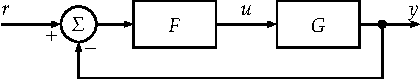
\includegraphics{feedback}
  \caption{\label{fig:feedback}%
    A simple illustration in a floating \envname{figure} environment.  Note that figure captions are always placed under the corresponding figure, and hence that the caption code should always appear at the end of the \envname{figure} environment.}
\end{figure}

\section{Hyperlinks}
%
For readers our the electronically published version of your thesis, as well as yourself while your are working on it, it is very convenient to have working hyperlinks in the document.

\subsection{Basic setup}
%
Basically, hyperlinks are obtained by using the \styname{hypreref} package. However, this package has quite a lot of compatibility issues with other packages, and knowledge about how to deal with these issues is coded into the \rtthesis class.  That is, all you should have to do to get hyperlinks in your document is to specify the \classoption{hyperref} option to \rtthesis.  The class options related to the linking infrastructure of the document are listed in \tableref{tab:hyperref}.

At the time of writing \rtthesis does not call \texcommand{hypersetup} with information about document title, keywords, and other information provided to \texcommand{setupThesis} (see \tableref{tab:setupThesis}).  If someone wants this, it shouldn't be hard to do.

\begin{table}[tbp]
  \centering
  \caption{\label{tab:hyperref}%
    Class options related to (hyper) linking infrastructure.}

  \begin{tabular}{l p{0.5\linewidth}}
    \toprule%
    \textbf{Class option} & \textbf{Meaning} \\
    \otoprule%
    \classoption{hyperref} & Turn on hyperlinks using the \styname{hyperref} package.  Default. \\
    \classoption{nohyperref} & Turn off hyperlinks, and compensate for commands no longer provided by the \styname{hyperref} package. \\
    \midrule%
    \classoption{backref} & Turn on bibliography back references.  Default. \\
    \classoption{nobackref} & Turn off bibliography back references.  (Currently required if you plan to use the features of \styname{bibunits}.)\\
    \bottomrule%
  \end{tabular}
\end{table}


\subsection{Hyperlinks and electronic publishing}
%
To make your dear hyperlinks survive all the way to the electronic publishing system, you may have to replace the file that is sent to e-press by LiU-tryck.  The problem is that LiU-tryck creates a compressed version of the file that is used in the printer, and the compression will remove nice features such as page numbers, hyperlinks, and bookmarks.  Fortunately, the guys at e-press seem to be understanding and will accept to publish a file that they receive directly from you.

\subsection{Page number formatting in the index}
%
If you use an index in your thesis, you will often want to change the formatting of certain page numbers in the index.  Without \styname{hyperref}, this could look like
{\verbatimsize
\begin{verbatim}
hyperlinks\index{hyperlinks|textit}
\end{verbatim}}
to get the page number for this occurrence of \emph{hyperlinks} to be typeset in italics.  The problem with this is that this page number will not be a hyperlink, while other page numbers will be hyperlinks to the correct page.  To get both italics and a hyperlink you need to define a special index formatting commands like the following.
{\verbatimsize
\begin{verbatim}
\newcommand{\hyperpageit}[1]{\textit{\hyperpage{#1}}}
\newcommand{\hyperpagebf}[1]{\textbf{\hyperpage{#1}}}
\newcommand{\hyperpagefootnote}[1]{\hyperpage{#1}n}
\end{verbatim}}

Now, you can write
{\verbatimsize
\begin{verbatim}
hyperlinks\index{hyperlinks|hyperpageit}
\end{verbatim}}
to get both italics and a hyperlink.  The \rtthesis class will provide a trivial definition of \texcommand{chapter} in case \styname{hyperref} is not loaded, so you may safely start to use the above definitions even if you are not sure whether you will use hyperlinks in the end.

\subsection{Friendlier hyperlinks}
%
The default mechanism for references in \LaTeX{}, being the command \texcommand{ref}, is modified as expected by the \styname{hyperref} package.  For instance, the number in “chapter~\ref{cha:rtthesis}” is linked to the beginning of the current chapter (if you click it, be sure to just the \emph{jump back} function of your \textsc{pdf} viewer to get back to here!).  However, all of “\hyperref[cha:rtthesis]{this}” is also a link to the same place.  That is, it is possible to other things than the number itself as links.  We could also make a reference that will never be linked, like in “chapter~\ref*{cha:rtthesis}”.

So, what's so friendly about this?  What I'm aiming at is that you can say “\hyperref[cha:rtthesis]{chapter~\ref*{cha:rtthesis}}”.  The code for this link is
{\verbatimsize
\begin{verbatim}
\hyperref[cha:rtthesis]{chapter~\ref*{cha:rtthesis}}
\end{verbatim}}

Of course, it is very annoying to repeat the key twice; first to point the hyperlink to the correct place, second to show the number of the chapter.  With the \texcommand{autoref} command from the \styname{hyperref} bundle, we get “\autoref{cha:rtthesis}”.  This is almost perfect.  The problem is that one cannot get an uppercase initial at the beginning of a sentence without redefining “chapter” to “Chapter“,
{\verbatimsize
\begin{verbatim}
\renewcommand{\Chaptername}{Chapter}
\end{verbatim}}
but then we will not get the nice lower case initial in the middle of a sentence.  Many authors don't bother about this and use uppercase initials irrespectively of where in a sentence the reference appears.

The only solution I (Henrik Tidefelt) knows of, is to define special commands for each type of reference.  A basic solution might look as follows.
{\verbatimsize
\begin{verbatim}
\newcommand{\chapterref}[1]{\hyperref[#1]{chapter~\ref*{#1}}}
\newcommand{\Chapterref}[1]{\hyperref[#1]{Chapter~\ref*{#1}}}
\end{verbatim}}

You should then use \texcommand{chapterref} in the middle of a sentence, and \texcommand{Chapterref} at the beginning of a sentence.  I you later decide that you want to have upper case initials everywhere, you just have to change your definitions to
{\verbatimsize
\begin{verbatim}
\newcommand{\chapterref}[1]{\hyperref[#1]{Chapter~\ref*{#1}}}
\newcommand{\Chapterref}[1]{\hyperref[#1]{Chapter~\ref*{#1}}}
\end{verbatim}}

A more complete solution will also provide commands for the plural forms “chapters” and “Chapters”.

It is also nice to use a similar technique for page references.  For instance, this chapter starts on \hyperref[cha:rtthesis]{page~\pageref*{cha:rtthesis}}, and such links can be created easily using a command like
{\verbatimsize
\begin{verbatim}
\newcommand{\pagepageref}[1]{\hyperref[#1]{page~\pageref*{#1}}}
\end{verbatim}}

Because of the many possible preferences for how to handle labels and references within documents, \rtthesis does not define any related commands.  The current section should give you some ideas of what can be achieved, and now it is up to you to design your own solution or borrow a solution from someone else (or simply stick with \texcommand{autoref} or the 1980's way of doing things)!

\section{Backreferences from the bibliography}
%
By default, \rtthesis uses the \styname{backref} package to put references from the bibliography back into the text.  The options for turning this feature on and off are listed in \tableref{tab:hyperref}.

By controlling this feature via the class, the choice whether to use it or not can be made orthogonal to the choice of whether to use \styname{hyperref} or not.

In addition to just loading \styname{backref}, \rtthesis will do a basic setup of the commands used to typeset the list of page numbers for each reference.  This behavior can easily be redefined without modifying the \rtthesis class file.  See the \styname{backref} documentation for details on how to do this!

\section{Using the \styname{bibentry} package}\label{sec:rtthesis:bibentry}
%
The \styname{bibentry} package makes it possible to use the information in the bibliography to present your publications at any place in the document.  In order to work independently of whether you use back references from the bibliography or not, you need to follow the pattern below each time you use the \texcommand{bibentry} command, where \texttt{KEY} is the same key to you publication that you would with use with any other citation command.

\begin{minipage}{1.0\linewidth}
  \verbatimsize
\begin{verbatim}
\begin{quotation}
  \nocite{KEY}\noindent
  \backrefparscanfalse\bibentry{KEY}.\backrefparscantrue
\end{quotation}
\end{verbatim}
\end{minipage}

To use the \envname{quotation} environment is just a suggestion — it will make the reference stand out by using a some what shorter text line width.  Note the period that follows the \texcommand{bibentry} command — the command leaves it up to you how to terminate the entry.  The \texcommand{nocite} command ensures that the reference appears in the bibliography, which is necessary to produce the entry.  The \texcommand{noindent} commands simply prevents the first line in the \envname{quotation} from being indented.  The commands \texcommand{backrefparscanfalse} and \texcommand{backrefparscantrue} are related to the \styname{backref} package used to produce back references from the bibliography, and should always surround the \texcommand{bibentry} command.  In case you have turned back references off using the \classoption{nobackref}, \rtthesis will provide substitutes for these two commands.


\section{Fonts}
%
Though basically not a task for a \LaTeX{} class, \rtthesis will assist in loading some font packages.  There are some class options that control this behavior, described below, and if these options are not good enough for you, you may have to make your own copy of the class and replace the font packages you don't like.  Options for font selection are listed in \tableref{tab:fonts}.

One reason, however, for letting \rtthesis handle the font selection is that this makes it possible for the class to do some things more intelligently.  At the moment, \rtthesis will help you make use of some of the goodies of KpFonts, if you choose to use that font.

\begin{table}[tbp]
  \centering
  \caption{\label{tab:fonts}%
    Class options related to fonts.  When slanted small caps are activated, theorem-like environments will use slanted text instead of italics.  The lower part of the table are examples of options that will be understood by the \styname{kpfonts} package, and are only meaningful in combination with the \classoption{kp} option.  (Note that options passed to \rtthesis, but that are not understood by \rtthesis will be passed on automatically by \LaTeX{} to loaded packages.)}

  \begin{tabular}{l p{0.5\linewidth}}
    \toprule%
    \textbf{Class option} & \textbf{Meaning} \\
    \otoprule%
    \classoption{kp} & Use KpFonts (Kepler) and activate slanted small caps.  Default.\\
    \classoption{times} & Use Times and deactivate slanted small caps.\\
    \classoption{lm} & Use Latin Modern and deactivate slanted small caps.\\
    \midrule%
    \classoption{largesmallcaps} & Let the small caps be slightly higher than an \emph{x}.  See the KpFonts documentation!\\
    \classoption{intlimits} & Placement of integration limits.  See the KpFonts documentation!\\
    \classoption{widermath} & Put just a little more horizontal space between entities in math mode.  See the KpFonts documentation!\\
    \bottomrule%
  \end{tabular}
\end{table}

\section{Hanging punctuation}
%
The \rtthesis class automatically loads the \styname{pdfcprot} package with its default settings.  It uses a pdf\TeX{} feature to make punctuation hang into the right margin.  If you don't like it, make your own copy of the class and comment out the line that loads the package.  One reason not to use it would be if your document will be (perhaps only occasionally) typeset using the old \TeX{} program, since this will lead to noticeable differences in the line breaks compared to when pdf\TeX{} is used.  No matter what you choose, make your choice \emph{before} you start working with the page breaks in your document!

\section{Paragraph breaks}
%
There are two common ways of visualizing paragraph breaks in a document, illustrated by the two examples below.  The look of paragraph breaks is controlled using the class options listed in \tableref{tab:parskip}.

\begin{table}[tbp]
  \centering
  \caption{\label{tab:parskip}%
    Class options related to formatting of paragraph breaks.}

  \begin{tabular}{l p{0.5\linewidth}}
    \toprule%
    \textbf{Class option} & \textbf{Meaning} \\
    \otoprule%
    \classoption{noparskip} & US style, see \exampleref{ex:paragraph-break-noparskip}.  Default.\\
    \classoption{parskip} & European style, see \exampleref{ex:paragraph-break-parskip}.\\
    \bottomrule%
  \end{tabular}
\end{table}

% \begin{example}[Default text]
%   This example does not mess with the lengths controlling the paragraph break format.  But you bet it ends in vmode!

% \end{example}

% It is good to see what it looks like if one puts text just below an example.

% \begin{example}[Default text]
%   This example does not mess with the lengths controlling the paragraph break format.  This one ends in hmode!
% \end{example}

\begin{example}[Indented first line]\label{ex:paragraph-break-noparskip}%
  \setlength{\parskip}{0pt}%
  \setlength{\parindent}{1.5em}%
  This style is still the most common.  It is particularly dominant in text written in the US.

  It is a matter of style whether to omit the indentation of the first line after a sectioning command such as \texcommand{chapter} or \texcommand{subsection}.  The omission is typically automated, but can also be enforced using the  \texcommand{noindent} command.

  One drawback of not having vertical space between paragraphs is that it will be harder for pdf\TeX{} to find good places for page breaks, compared to the option shown below.  If you like compact documents, however, this is the option for you!

  For testing purposes, this example ends with a paragraph break, so that \TeX{} is in \emph{vmode} at the end.  You should always avoid this, but the class will try to compensate for your mistakes\ldots

\end{example}

\begin{example}[Vertical white space]\label{ex:paragraph-break-parskip}%
  \setlength{\parskip}{1ex}%
  \setlength{\parindent}{0pt}%
  This style is still increasing in popularity.  It is rather common in modern texts written in Europe, and the style has received special attention from the Netherlands \TeX{} user group \emph{Nederlandstalige \TeX{} Gebruikersgroep, \textsc{ntg}}.  Their efforts can be used through their variants of the standard \LaTeX{} classes.

  Unfortunately, the \textsc{ntg} classes are not compatible with \rtthesis, and the solution provided by the \styname{parskip} package is only part of the solution.  Hence, \rtthesis will do more than just loading the \styname{parskip} package for you if you specify the \classoption{parskip} option.

  A good reason to put code related paragraph breaks in the class file is that all the small adjustments that different people come up with can be put in one placed so that they are accessible to future users of the class.
\end{example}

\section{Page breaks}\label{sec:tipt:page-breaking}
%
There is a whole lot to say about how to obtain nice page breaks.  You will find some recommendations below, but do not use this document as your ultimate reference on this topic!  (This document itself contains some really nasty page breaks --- at least at the time of writing this --- as a result of not paying any attention at all to the problem.  It would simply bee too time-consuming to keep adjusting the page breaks each time the document is edited.)
\begin{itemize}
\item
  Take no consideration of page breaks until page breaking is the only aspect of your thesis that remains to be taken care of!  Page breaking involves a lot of manual intervention of the automatic mechanisms in pdf\TeX{}, and as soon as you have started to intervene, any further changes to the text will risk to ruin your page breaking fixes, and may even lead to worse results than before since the automatic page breaking has been tampered with.
\item
  First thing to try is to make changes to the text to help the automatic page breaking mechanism.  Try to make sentences longer or shorter depending on the situation.  Since this will not tamper with the automatic page breaking mechanism, this option will incur the least loss of maintainability of your document.
\item
  Can the location of floats be changed to improve page breaks?  Play around with exactly where in your source files the code for the floating environments appears!
\item
  You may also try to force early page breaks using the \texcommand{Needspace*} command.  For instance, putting
{\verbatimsize
\begin{verbatim}
\Needspace*{2\baselineskip}
\end{verbatim}}
before a paragraph will cause a page break if there is not enough vertical space on the page to hold two lines of text.  The good thing about this option is that your intervention will cause no harm if the \texcommand{Needspace*} command appears in the middle of a page.  The bad thing about this option is that it may cause remaining vertical space on the broken page to be stretched quite badly.  You should always check that the resulting page looks OK!

For more information, and related commands, see the documentation for the \styname{needspace} package!
\item
  The last option is to play with the vertical size of individual pages.  For instance, putting
{\verbatimsize
\begin{verbatim}
\enlargethispage{2\baselineskip}
\end{verbatim}}
before a paragraph you would like to fit into the current page will make space for two extra lines of text.  This avoids the bad stretching of vertical space that the \texcommand{Needspace*} option may cause.  However, if you would make other changes that makes tampering with the page size unnecessary, it will be very time-consuming to detect this and remove the no longer needed \texcommand{enlargethispage} command.
\end{itemize}

Note that manual page breaking is a time-consuming task.  Make sure to have at least one full day allocated to page breaking before you submit your thesis for print!

\section{Input encoding}
%
Two input encodings are supported, being \mbox{latin-1} and \mbox{\textsc{utf}-8}.  The choice of input encoding should be made via the \rtthesis class, so that the class can use the correct encoding to define certain global strings.  The input encoding options are listed in \tableref{tab:inputenc}.

\begin{table}[tbp]
  \centering
  \caption{\label{tab:inputenc}%
    Class options related to input encodings.  Note that there is no default; \rtthesis requires one of these options to be passed explicitly.}

  \begin{tabular}{l p{0.5\linewidth}}
    \toprule%
    \textbf{Class option} & \textbf{Meaning} \\
    \otoprule%
    \classoption{latin1} & Simply use \styname{inputenc} with option \classoption{latin1}. \\
    \classoption{utf8} & Use \styname{inputenc} with option \classoption{utf8}, and define some additional characters. \\
    \bottomrule%
  \end{tabular}
\end{table}

Choose \mbox{latin-1} if you depend on lots of files using this encoding, and do not want to change the encoding of these files.  Changing the encoding of a file is easy both in Emacs and using the \emph{iconv} command line utility.  The \mbox{latin-1} encoding is the default in \rtthesis, but the choice can be made explicit by passing the \classoption{latin1} option to the class.

Choose \mbox{\textsc{utf}-8} to be able to type many more characters directly in your \LaTeX{} sources compared to \mbox{latin-1}.  For instance, names of foreign authors often use characters that cannot be entered directly using \mbox{latin-1}.  In \mbox{\textsc{utf}-8}, most of these as well as special punctuation characters such as double quotes and various dashes can be entered directly in the source.  Use the \classoption{utf8} class option if your files are encoded in \mbox{\textsc{utf}-8}.

The current implementation of \mbox{\textsc{utf}-8} in the \styname{inputenc} package only defines the input encoding for characters that have corresponding glyphs in active fonts (see the \styname{inputenc} documentation for details).  This means that some characters that \TeX{} would build by combining several glyphs will not be defined by \styname{inputenc}.  If the \classoption{utf8} is given, \rtthesis will define a list of additional characters by inclusion of the package \styname{rtthesis-utf8-ext}.  If you need additional characters, you should make your own package similar to \styname{rtthesis-utf8-ext}, and then let the maintainer of \rtthesis know, so that the additional characters may be added to \styname{rtthesis-utf8-ext} so that others can use them in the future.  Note that \styname{rtthesis-utf8-ext} may be a useful package also when you are not using the \rtthesis class.

It is easy to set up Emacs so that it uses the \mbox{\textsc{utf}-8} encoding for your \TeX{} files, but it is out of the scope of the current document to give further explanations here.


\section{\rtthesis and \styname{natbib}}
%
Interoperability with different bibliography packages is a tricky issue.  It has been a design decision to try to support at least \styname{natbib}, at the cost of loosing compatibility with other packages such as \styname{jurabib}.  The core of the problem is package loading order, requiring \styname{natbib} to be loaded very early on in the class.  To pass options to \styname{natbib}, pass them as global class options to \rtthesis.  Note that the default options for \styname{natbib} are quite reasonable, and see \tableref{tab:natbib} for examples of other options that \styname{natbib} will pick up.  If you know how to resolve the conflict with the \styname{natbib} option \classoption{usebibunits}, let the \rtthesis maintainer know!

\begin{table}[tbp]
  \centering
  \caption{\label{tab:natbib}%
    Class options related to the \styname{natbib} package.  Note that options can be passed to \styname{natbib} by passing them as global class options to \rtthesis.  See the \styname{natbib} documentation for more useful options.}

  \begin{tabular}{l p{0.5\linewidth}}
    \toprule%
    \textbf{Class option} & \textbf{Meaning} \\
    \otoprule%
    \classoption{authoryear} & Default option of \styname{natbib} --- no need to specify.\\
    \classoption{round} & Default option of \styname{natbib} --- no need to specify.\\
    \classoption{colon} & Default option of \styname{natbib} --- no need to specify.\\
    \midrule%
    \classoption{square} & Example of option that \styname{natbib} will pick up (alternative to \classoption{round}).\\
    \classoption{comma} & Example of option that \styname{natbib} will pick up (alternative to \classoption{colon}).\\
    \midrule%
    \classoption{numbers} & Conflicting \styname{natbib} option --- forbidden in combination with \classoption{usebibunits}, see \classoption{forcenumbers} below.\\
    \classoption{forcenumbers} & Enforce option \classoption{numbers} to be passed to \styname{natbib} (alternative to \classoption{authoryear}) --- it's up to you to resolve the conflict.\\
    \bottomrule%
  \end{tabular}
\end{table}


\section{The lists of previous theses}
%
The lists of previous licentiate's and PhD theses can be found in \textfilename{liclist.tex} and \textfilename{phdlist.tex}, respectively, and the appropriate one of the is automatically included at the end of your thesis.  Both files are found in the directory\\
\textfilename{\$TEXMFGROUPLOCAL/tex/latex/rt/rtthesis} .

Note that it is \emph{your responsibility} to make sure that your thesis is added to the appropriate list after you have sent it to print but before the next thesis of the same kind is printed.  If other people are writing theses at the same time as you, you will have to coordinate your moves in order to make sure that the lists get updated in the correct order.  To get your thesis added to the appropriate list, you simply send an email with information about your thesis to the \rtthesis maintainer.  The information shall be in one of the following formats:

{\verbatimsize
\begin{verbatim}
\licitem{J.~Doe}{Title}{Thesis No}{YYYY}
\end{verbatim}}

or

{\verbatimsize
\begin{verbatim}
\phditem{J.~Doe}{Title}{Theis No}{YYYY}{ISBN}
\end{verbatim}}

It is a good idea to make a copy of the file you need when it is time to print.  If you don't make a copy, and then compile your thesis again at a later time, the list will be wrong because it will include at least one thesis that wasn't prior to yours — namely your own!


\section{Compilation theses}
%
The \rtthesis class aims to support the production of both monographs and compilation theses.  There is a compilation thesis example included with \rtthesis.  Please have a look at that while reading the sections below!


\subsection{Including publications in your thesis}
%
It is assumed that included publications shall be compiled together with the rest of your thesis, as opposed to being included as exactly the way the look where published.  Under this assumption, it is reasonable to expect things such as a suitable chapter numbering, and that the global table of contents includes the sections withing publications.  Note that it would be rather difficult to get things such as the table of contents and other infrastructure right if publications were to be included by direct \textsc{pdf} inclusion.

The \envname{papers} environment provided by \rtthesis will redefine commands and set up some additional commands to support the inclusion of \LaTeX{} sources of your publication.  It is recommended that the environment is placed in a second part of the thesis.  Inside the environment, the \texcommand{chapter} command is redefined to both start a new chapter and set up the title of the publication to be included in the same chapter.  Chapters will be labeled with letters instead of numbers, so it is up to you to make a clear distinction between referencing an appendix chapter and a publication chapter.

If the title of a publication is too long to fit in the page header, you may follow the \texcommand{chaptermark} command by a \texcommand{chaptermark} command.  Since the \texcommand{chaptermark} command takes an optional argument to be used in the table of contents, there are three different variations of the publication title that can be defined.

The word for publications used by \rtthesis is \emph{paper}; it will appear both on the chapter title page and in page headers.  To change this to something else, you simply have to redefine \texcommand{chaptername} to something else inside the \envname{papers} environment.

After setting up the publication title, the \texcommand{author} command should be used to set up the list of authors.  It works as usual, but sports two special \rtthesis commands that should be used when there are two author affiliations;  put \texcommand{authorleft} immediately after author names who's affiliation should appear to the left below the list of authors, and put \texcommand{authorright} after the other authors.  There is currently no support for more than two different affiliations.

In case there is only one affiliation, that affiliation is given by \texcommand{paperaffiliation} (which should be set once and for all to your own affiliation), and you use the \texcommand{email} command to specify the list of email addresses to the authors.

In case of two affiliations, you call the commands \texcommand{affilblockleft} ,\texcommand{affilblockright}, \texcommand{emailleft}, and \texcommand{emailright} with the appropriate arguments.  Note that one of the two affiliation block arguments should simply be \texcommand{paperaffiliation}.

Additional information about the publication is given in after \texcommand{item} commands inside the \envname{paperinfo} environment.  In addition to the items given, the environment automatically starts with one item displaying the author information (without any marks related to affiliation blocks).  Three commands are defined by \rtthesis to simplify consistent formatting of additional information.
\begin{itemize}
\item \texcommand{paperedited{\emph{bib-key}}} — For ordinary publications.  The extent to which the publication has been edited should be state clearly.  The bibliography entry will be formatted using the technique described in \sectionref{sec:rtthesis:bibentry}.
\item \texcommand{paperprelver{\emph{ISY-report-number}}} — For publications for which there is only a preliminary version available.  The preliminary version should be published as a technical report at the department, and as no bibliography keys are involved, the technical report will not be listed in any the bibliography.
\item \texcommand{papertechrep{\emph{ISY-report-number}}} — For publications that are not yet even preliminary versions of something.  These too should be published as technical reports at the department, and will not appear in the bibliography.
\end{itemize}

At this point the chapter title page will be finished.   The next step is to make a nice title and abstract for your publication on the following odd page.  Use \texcommand{maketitle} or \texcommand{maketitletwoaffil} depending on whether you set up one or two affiliation blocks.  Then put the publication abstract inside the \envname{abstract} environment.

After this point, you should just be able to include the source of your publication, with \texcommand{section} as the topmost sectioning command (since the publication itself is a chapter of your thesis).

Finally, you must decide where your references should go.  Should there be one global bibliography for the whole thesis, or should there be one bibliography for each publication.  This is the topic of the next section.

\subsection{Compilation theses and bibliographies}
%
If you are fine with having just one global bibliography for the whole thesis, everything should work out of the box.  Hence, this section will try to describe how to do in order to get one bibliography for the background part of your thesis, and one for each publication.

The \rtthesis class only supports this by relying on the \styname{bibunits} package.  Due to package loading order issues, it should always be loaded by passing \classoption{usebibunits} to \rtthesis.  Note that some of the \styname{bibunits} commands appears to be incompatible with bibliography back references, so you need to pass the \classoption{nobackref} to \rtthesis if you plan to use the \styname{bibunits} features.

\begin{remark}
  There is a very interesting package called \styname{biblatex} which is currently in beta version.  Hopefully, it will let us drop the messy packages \styname{bibunits} and \styname{backref}.  You are invited to try this package, and if you find it to work satisfactory it should probably be incorporated in \rtthesis.  Future maintainers of \rtthesis are strongly encouraged to find out what \styname{biblatex} can do for us!
\end{remark}

Use the command \texcommand{defaultbibliography} to specify the bibliography files to use for all of the per-publication bibliographies, and use \texcommand{defaultbibliographystyle} to select the bibliography style, see the \styname{bibunits} documentation for details.

To get an individual bibliography for a publication, you should just have to include that chapter in a \envname{bibunit} environment, and call \texcommand{putbib} where you want the bibliography to appear.  Here, the \texcommand{putbib} command will be redefined by \rtthesis in order to make the bibliography appear in the table of contents.

A bibliography for references that appear in the background part of your thesis are produced as usual with the \texcommand{bibliography} command.  (It might be good to know that \rtthesis will automatically issue the \texcommand{nobibliography*} command in order to make the \styname{bibentry} package work as you would expect.)

\section{Master's theses}\label{sec:msc}
%
The \styname{liuthesis} class by Gustaf Hendeby was developed for the production of master's theses at Linköping University.  The class knows how to create the special pages required by several departments, and in the summer of 2011 this capability was merged into \rtthesis.  This makes it convenient to produce a master's thesis at Linköping University using \rtthesis instead of \styname{liuthesis}, allowing a wider audience to benefit from the more active development of \rtthesis.\footnote{The \LaTeX{} class files tend to be maintained by PhD students, and PhD students have a tendency to be more interested in maintaining the class files for writing licentiate's and PhD theses than class files for master's theses.}

This section describes how to use \rtthesis to produce a master's thesis.  To begin, pass \emph{msc} as the value for the key \emph{type} in the call to \texcommand{setupThesis}, and select your department using the key \emph{department}.  More details are given below, and the reader is encouraged to study the bundled example in order to get a better overall picture.

\subsection{Master's thesis setup}
%
In addition to the pieces of information given to \texcommand{setupThesis} for licentiate's and PhD theses (see \tableref{tab:setupThesis}), there are some that only apply to master's theses.  These are listed in \tableref{tab:setupThesis-msc}.

\begin{table}[tbp]
  \centering
  \caption{\label{tab:setupThesis-msc}%
    \texcommand{setupThesis} key-value pairs for master's theses, in addition to those listed in \tableref{tab:setupThesis}.  Note that values that include white space are surrounded by braces.}

  \begin{tabular}{>{\ttfamily}r !{\texttt{=}} >{\ttfamily}l l}
    \toprule%
    \textbf{Key} & \textbf{Example value} & \textbf{Comment} \\
    \otoprule%
    swetitle & \{Svensk titel\} & Title in Swedish\\
    swesubtitle & \{Bra grejer\} & Optional Swedish subtitle\\
    month & 4 & \\
    day & 9 & \\
    subject & reglerteknik & \\
    site & \{Bosses AB i Linkan\} & \\
    division & \{Avdelningenrt\ldots\} & \\
    department & isy & See \tableref{tab:department} \\
    examiner & \{Lena Lärare\ldots\} & Details given below \\
    supervisor & \{Doktorand Si\} & Details given below \\
    keywords & \{this, that\} & Appears on library page \\
    isrn & LiTH-ISY-EX\ldots & See below \\
    url & \{http://\ldots\} & Thesis download \textsc{url}, see below \\
    \bottomrule%
  \end{tabular}
\end{table}

The value for the key \emph{department} must be one of the special values listed in \tableref{tab:department}.  This setting controls both the department name and address, as well as how the special pages of the thesis are formatted.  Please help the \rtthesis maintainer to keep the special pages for your department up to date.

In the values for the keys \emph{examiner} and \emph{supervisor}, multiple persons should be separated using \texcommand{AND}, and the affiliation of a person should appear after \texcommand{AT}, like this:
{\verbatimsize
\begin{verbatim}
  supervisor={Doktorand Si \AT \textsc{isy}, Linköpings universitet
         \AND Ingenjör Så \AT Företaget},
\end{verbatim}}

The \textsc{isrn}\footnote{The \textsc{iso} standard for \textsc{isrn} was withdrawn in 2007, but the report numbering system is still in use at Linköping University.} should be something like
{\verbatimsize
\begin{verbatim}
  isrn=LITH-ISY-EX-{}-YY/NNNN-{}-SE
\end{verbatim}}
but the format varies between different departments.  Note that if the report identifier contains two or three consecutive dashes, they have to be separated by empty braces in the input to prevent \LaTeX{} from interpreting them as one character.  The thesis download \textsc{url} should be something like
{\verbatimsize
\begin{verbatim}
  url={http://urn.kb.se/resolve?urn=urn:nbn:se:liu:diva-XXXXX}
\end{verbatim}}
The exact details regarding the report number and \textsc{url} will be given to you by the librarian when you register your thesis.

\begin{table}[tbp]
  \centering
  \caption{\label{tab:department}%
    Recognized values for the key \emph{department} in \tableref{tab:setupThesis-msc}.}

  \begin{tabular}{>{\ttfamily}c p{0.45\linewidth} l}
    \toprule%
    \textbf{department} & \textbf{Department of\ldots} & \textbf{Updated}\\
    \otoprule%
    ida & Computer and Information Science & Not after 2008-08-01\\
    ifm & Physics, Chemistry and Biology & 2011-07-03\\
    iei & Management and Engineering & \emph{Out of date!}\\
    isy & Electrical Engineering & 2011-07-03\\
    itn & Science and Technology & 2011-07-03\\
    mai & Mathematics & 2011-07-03\\
    \bottomrule%
  \end{tabular}
\end{table}

\subsection{Special pages}
%
The requirements on a master's thesis include that certain information go on the front page and title page of the thesis.  Further, a library page for cataloging purposes is required at the beginning of the thesis, and a page with copyright information is required at the end.  The copyright page is automatically added at the end.  The other special pages can be produced using the macros \texcommand{makeFrontPage}, \texcommand{maketitle} (as usual), and \texcommand{makeLibraryPage}.  These macros are meant to be invoked more or less immediately after \texcommand{begin\{document\}}, see the bundled example for details.  Note that in the printed report, the front page should be replaced by the cover, and the library page is \emph{probably} meant to be on a loose piece of paper inserted between the cover and the title page.

There is no magic that puts the correct abstract on the library page, but the abstract must be given as an argument to \texcommand{makeLibraryPage}.  To make sure that this is exactly the same as the abstract in the thesis, it is recommended that you write the abstract text without any surrounding \envname{abstract} environment in a separate file, say \textfilename{svensk-sammanfattning.tex}.  Then you can use this file twice, like this:
{\verbatimsize
\begin{verbatim}
\makeLibraryPage{Svensk sammanfattning här.
}

\begin{abstract}[swedish]
  Svensk sammanfattning här.

\end{abstract}
\end{verbatim}}
(The bundled example uses this technique.)

\subsection{Choice of language}
%
If your main report language will be Swedish, put
{\verbatimsize
\begin{verbatim}
\selectlanguage{swedish}
\end{verbatim}}
right after
{\verbatimsize
\begin{verbatim}
\begin{document}
\end{verbatim}}
Also make sure to provide the thesis title (and possibly subtitle) in Swedish via the keys \emph{swetitle} and \emph{swesubtitle} to \texcommand{setupThesis}.  You may then omit writing an abstract in English.

If your main report language will be English you don't need to change the default choice of language.  However, you must provide a thesis title both in English and Swedish, and the thesis should contain abstracts in both English and Swedish.


\section{Compiling the document}
%
Using all the current features of \rtthesis, the following sequence of steps is usually sufficient to compile your document.  Let us assume your main file is named \textfilename{main.tex}.
\begin{itemize}
\item
  First run
{\verbatimsize
\begin{verbatim}
pdflatex main
\end{verbatim}}
  to scan your document for references, labels, and index items.
\item
  Then run
{\verbatimsize
\begin{verbatim}
bibtex main
\end{verbatim}}
  to extract relevant references from your bibliography file(s).  If you are using the \styname{bibunits} package, you also have to process some additional files;
{\verbatimsize
\begin{verbatim}
bibtex bu1; bibtex bu2; ...; bibtex bun
\end{verbatim}}
\item
  If you have an index in your document, run
{\verbatimsize
\begin{verbatim}
makeindex main
\end{verbatim}}
  to format it.
\item
  Then run
{\verbatimsize
\begin{verbatim}
pdflatex main
\end{verbatim}}
  to insert references in the typeset document.  This will typically move things around, and your page references will be invalidated.
\item
  Hopefully, it is enough to run
{\verbatimsize
\begin{verbatim}
pdflatex main
\end{verbatim}}
  once more now to get the page references right.  You will get a warning if you need to repeat this step.
\end{itemize}

In addition to the steps above, certain auxiliary files must be deleted when certain features of the class are turned on or off.  In particular, turning hyperlinks on or off requires the following.
{\verbatimsize
\begin{verbatim}
rm main.aux main.toc main.ind
\end{verbatim}}

\section{Generating a thesis cover and the “spikblad”}
%
A thesis cover can be created by making a file that contains the \texcommand{makecover} command.  For example, given that \textfilename{mythesis.sty} invokes the \texcommand{setupThesis} command with the necessary information (see \tableref{tab:setupThesis}), a PhD thesis cover can be made as follows.

\begin{minipage}{1.0\linewidth}
  \verbatimsize
\begin{verbatim}
\documentclass[utf8,phd]{rtthesis}
\usepackage{mythesis}

\makecover
\end{verbatim}
\end{minipage}

Note that while all licentiate's theses should have the same cover, there is no standard (but many rules set by the university!) for the PhD theses.  The \texcommand{makecover} command gives a “classic” cover that quite a few people have used over the years.  This cover might also be useful as a means to compile the information needed when LiU-Tryck (or some other printing company) designs a more artistic cover.

For a dissertation, there should always be a “spikblad” (literally, \emph{nailing sheet}).  Such an information sheet can be generated easily if the English abstract is put in a separate file.  In this case, the same abstract can be included both in the thesis and in a separate file that defines the “spikblad”.  For a licentiate's thesis presentation, a similar information sheet should be produced.  The monograph example demonstrates how to created these, see the files \textfilename{spikblad.tex} (for dissertations) and \textfilename{licinfo.tex} (for licentiate's thesis presentations).


\section{Required logotypes (not included with \rtthesis)}
%
\Tableref{tab:logos} lists files with logotype graphics that are needed by \rtthesis.  They are not part of the \rtthesis bundle since they are used in many other contexts as well.  Users at the Division of Automatic Control should have access to these files via the group's common texmf tree, but in order to be able to work at home you will have to make sure one way or another that the files are installed.

Beware that the university changes logos quite often. Make sure that there are no new versions of the logos you use.  If the logos are old, please, let the \rtthesis maintainer know so that the files get updated at the central location.

\begin{table}[tbp]
  \centering
  \caption{\label{tab:logos}%
    Files with logotype graphics used by \rtthesis.  Use the command \texttt{kpsewhich} to find where the files are located!}

  \begin{tabular}{l p{0.5\linewidth}}
    \toprule%
    \textbf{Filename} & \textbf{Use} \\
    \otoprule%
    \textfilename{LinkUniv\usc{}sigill\usc{}sv.pdf} & For the cover and the first page in PhD theses.\\
    \textfilename{LiTH\usc{}staende\usc{}eng\usc{}sv.pdf} & For the cover of both licentiate's and PhD theses.\\
    \textfilename{rtlogo\usc{}tall.pdf} & For the first page in licentiate's theses.\\
    \bottomrule%
  \end{tabular}
\end{table}

\section{Compatibility with standard packages}
%
Incompatibilities between different packages is a problem that quickly becomes quite an issue when the list of packages used in a document grows beyond just a few.  It may sound strange, but it is because of compatibility problems that \rtthesis includes a rather long list of packages for you.  The reason is that this allows knowledge about package loading order requirements and various workarounds, to be encoded in the class file.

No list of packages included by \rtthesis will be presented here, but you should check the class file directly to be sure that you always get the correct answer to whether a package is included or not (or you can just read the compilation output).

Packages with no known compatibility issues will generally not be included by \rtthesis unless needed by the class itself.  The following list contains some examples of useful packages that are not included by \rtthesis.  They \emph{should} be compatible with \rtthesis.  Please let the \rtthesis maintainer know if any of these are no longer compatible, or if you have suggestions for other packages that should be mentioned here.
\begin{itemize}
  \item \styname{nextpage} — page break control
  \item \styname{algorithm} — code listings
  \item \styname{listings} — code listings
  \item \styname{SIunits} — physical dimensions
  \item \styname{pmat} — partitioned matrices
  \item \styname{bm} — bold math
  \item \styname{footmisc} — extras for footnotes
  \item \styname{dcolumn} — decimal point alignment in tables (the already included \styname{array} can also do this)
  \item \styname{lettrine} — start chapter with fancy letter
  \item \styname{supertabular} — multi-page tables
  \item \styname{longtable} — multi-page tables
  \item \styname{multirow} — tabular entries occupying more than one row
\end{itemize}


\part*{Appendix}
\appendix
\chapter{Appendix 1}\label{cha:appendix1}

%Enkäter, intervjufrågor, omfattande tabeller med mätvärden, omfattande beräkningar eller programkod kan med fördel presenteras som bilagor.
%Huvuddragen i resultaten ska naturligtvis presenteras i rapportdelen, men för att läsaren själv ska kunna värdera resultaten kan dataunderlaget redovisas i bilagorna.

Detta är ett appendix-kapitel.  Jämför med appendixet i \chapterref{cha:Research}.

\section{Original Time Plan and Activities}
% en tidplan för examensarbetets genomförande inklusive planerade datum för halvtidskontroll och framläggning

\subsection{Before Uganda}

\begin{center}
    \begin{tabular}{ | l | p{10cm} |}
    \hline
    Week & Focus \\ \hline
    2 & Workshop with Lena Tibell and Konrad Schönborn on Research questions \& Proposal of method. \\ \hline
    3 & Start writing "Planeringsrapport".
    Study interaction design
    via guest lecture Jonas Löwgren,
    and reading the book "Thoughtful Interaction Design". \\ \hline
    4 & Interview with Take Aanstoot, Social entrepreneur in Kenya. Submission "Planeringsrapport". Education day in Service design in Stockholm (by Expedition Mondial). Meet Joachim Svärdh about Entrepreneurship research. \\ \hline
    5 & Approval "Planeringsrapport" with Camilla Forsell. Meeting with Lena Tibell and Konrad Schönborn (2016-02-02). Travel to Uganda. \\ \hline

    \end{tabular}
\end{center}

\subsection{In Uganda}

Times specified are in local time to where the master thesis was done at the time. Uganda time (EAT - Eastern Africa Time) is 2 hours forward of Swedish time (CET - Central European Time). Meetings with Swedish partners are generally done via Skype, where Uganda meetings are preferably done in person. Note that during all of this time, writing the master thesis will progress. After the time in Uganda, the report will be a 100\% focus. 1 day per week will be spent on report writing, including Analysis work for the meetings.

\begin{center}
    \begin{tabular}{ | l | p{10cm} |}
    \hline
    Week & Focus \\ \hline
    6 & \textbf{Cultural adaption}. Land, set up wifi, set up the apartment, learn about the YoungDrive organization, meet people. Be prepared for stomach disease. Get familiar with the transportation system in Kampala. Get familiar with the city.

    \textbf{Iteration 1}. Prepare Iteration 1 with Iliana. % sätta plan och förutsättningar för Iteration 1 (sätta i kontakt med coacher eller coach-möte, inleda kontakt om jag kan följa med ut i fält). Briefa Iliana i min projektplan.
    Start-up meeting with partners. % Uppstartsmöte. Ta del av deras kunskap, dröm, målbild - stämma av så att vi står på samma sida. Lyssna på områden inför frågeguiden.  % Lärdom från Kenya, att boka möte med Iliana och Josefina, projektledare, och gå igenom noggrant med stakeholders
    Start report writing: analyze, collect material, sort, structure and plan.
    % Analysera, samla stoff, sortera, strukturera och planera
    \\ \hline
    7 & \textbf{Iteration 1}. Prepare Interactions. Analyze Start-up meeting with partners. Write on report. % hypoteser vad vi tror att utmaningen är.
    in order to create \textit{Questionnaire guide}. Understand technical tools, without working on an app solution - the goal is to get familiar with the tools. % (öppen, undersökande, ej specifika frågor untan diskusionsunderlag). Göra backend.
    \\ \hline
    8 & \textbf{Iteration 1}. Travel for Interactions. Do 8 face-to-face interviews, with no digital focus, hypothetical situations. Do minimum 2 field visits to understand the coach's situation, ideally living in Kamuli or Tororo a couple of days. This is a good opportunity to learn coaches how the tablets and smartphones work.  \\ \hline % "jaså, det är så här det går till". Jag kommer få insikten "vänta nu, är det så här det går till?".

    9 & \textbf{Iteration 1}. Analysis \& Compilation. Thursday: Expert meeting (March 3rd, 6-7 PM). Friday: Partner meeting (March 4th, 11-12 AM).

    \textbf{Iteration 2}. Determine Needs. Ideation. Create low-fi Trigger material (pen and paper) and determine what the hi-fi (digital app) material should be.
    % Några coacher kanske verkar självgående, andra behöver mycket stöd. Det verkar som om den behöver fungera offline och online. Utifrån analysen skapar jag en egen behovsbeskrivning, sedan kreations-fas då jag kommer på idéer. Sedan gör jag ett low hi-fi triggermaterial, och det detaljerade triggermaterialet min digitala lösning.
    \\ \hline
    10 & \textbf{Iteration 2}. Design and Develop the hi-fi trigger material. \textit{Half-time check-up with examiner.} \\ \hline
    11 & \textbf{Iteration 2}. Interactions, control group \#1 \& \#2. \\ \hline
    12 & \textbf{Iteration 2}. Interactions, control group \#1 \& \#2. % Några gör jag på huvudkontoret med 8 personer. Några tar jag med mig trigger-materialet till, ut på fält.
    \\ \hline
    13 & \textbf{Vacation}. \\ \hline
    14 & \textbf{Iteration 2}. \textit{Analysis \#2} (What choices needs to be made? What path should be taken? Start formulate Customer path. If needed, document how people see apps, document limitations, document experience needs, document risks.) % Kundresa: ("What does a day/session look like for a coach? What are their basic needs?").
    \& Compilation. Thursday: Expert meeting (April 7th, 4 PM). Friday: Partner meeting (April 8th, 11-12 AM). Continued Development Creative Brief. Determine what actions needs to be taken outside of the development of the app. Create Behovsgrupper. \\ \hline

    15 & \textbf{Iteration 3}. Develop and Modifications phase. \\ \hline
    16 & \textbf{Iteration 3}. Develop and Modifications phase. Interactions: App Tests with Interviews \& Measurements (with time allocated for late arrivals and missing participants). \\ \hline
    17 & \textbf{Iteration 3}. Interactions: App Tests with Interviews \& Measurements.
    Analysis \& Compilation.
    Friday: Partner meeting (April 29th, 11 AM) \& Expert meeting (April 29th, 4 PM). \\ \hline
    18 & \textbf{Final analysis}. Finalize the app. Travel back to Sweden. \\ \hline
    \end{tabular}
\end{center}

\subsection{After Uganda}
\begin{center}
    \begin{tabular}{ | l | p{10cm} |}
    \hline
    Week & Focus \\ \hline
    19 & Write on Master thesis report. Attend Auscultations. \\ \hline
    20 & Write on Master thesis report. Attend Auscultations. \\ \hline
    21 & Write on Master thesis report. Attend Auscultations. Find opponent for Master thesis. \\ \hline
    22 & Submission of report to examiner, after approval by supervisor. Examiner decides on date and time for presentation. Send report to opponent, and get the opponent's report. \\ \hline
    \end{tabular}
\end{center}

\subsection{After Semester}

\begin{center}
    \begin{tabular}{ | l | p{10cm} |}
    \hline
    Week & Focus \\ \hline
    35 & Presentation of Master thesis, with supervisor, examiner and opponent. Hand over publication approval to the administrator. \\ \hline
    36 & Opposition of another person's Master thesis. \\ \hline
    37 & Do changes to report if requested. Upload report to X-sys for approval (within 10 days). Write Reflections document and submit on X-sys within the 10 days. Publish master thesis in X-sys. \\ \hline
    \end{tabular}
\end{center}


\section{Half-Time Evaluation Time Plan}

\backmatter

\bibliographystyle{plain}
\bibliography{IEEEfull,references/myrefs}

\printindex

\end{document}
